%%% Exemplo de utilização da classe ITA
% * <rodrigo.aragao.santos@gmail.com> 2018-07-04T00:55:14.659Z:
%
% ^.
%%%
%%%   por        Fábio Fagundes Silveira   -  ffs [at] ita [dot] br
%%%              Benedito C. O. Maciel     -  bcmaciel [at] ita [dot] br
%%%              Giovani Volnei Meinertz   -  giovani [at] ita [dot] br
%%%    	         Hudson Alberto Bode       -  bode [at] ita [dot]br
%%%    	         P. I. Braga de Queiroz    -  pi [at] ita [dot] br
%%%    	         Jorge A. B. Gripp         -  gripp [at] ita [dot] br
%%%    	         Juliano Monte-Mor         -  jamontemor [at] yahoo [dot] com [dot] br
%%%    	         Tarcisio A. B. Gripp      -  tarcisio.gripp [at] gmail [dot] com
%%%    	         
%%%
%%%  IMPORTANTE: O texto contido neste exemplo nao significa absolutamente nada.  :-)
%%%              O intuito aqui eh demonstrar os comandos criados na classe e suas
%%%              respectivas utilizacoes.
%%%
%%%  Tese.tex  2016-08-25
%%%  $HeadURL: http://www.apgita.org.br/apgita/teses-e-latex.php $
%%%
%%% ITALUS
%%% Instituto Tecnológico de Aeronáutica --- ITA, Sao Jose dos Campos, Brasil
%%%                   http://groups.yahoo.com/group/italus/
%%% Discussion list: italus {at} yahoogroups.com
%%%
%++++++++++++++++++++++++++++++++++++++++++++++++++++++++++++++++++++++++++++++
% Para alterar o TIPO DE DOCUMENTO, preencher a linha abaixo \documentclass[?]{?}
%   \documentclass[tg]{ita}			= Trabalho de Graduacao
%   \documentclass[tgfem]{ita}	= Para Engenheiras
%   								msc     		= Dissertacao de Mestrado
%   								mscfem   		= Para Mestras
%   								dsc      		= Tese de Doutorado
%   								dscfem   		= Para Doutoras
%   								quali    		= Exame de Qualificacao
%   								qualifem 		= Exame de Qualificacao para Doutoras
% Para 'Draft Version'/'Versao Preliminar' com data no rodape, adicionar 'dv':
%   \documentclass[dsc, dv]{ita} 
% Para trabalhos em Inglês, adicionar 'eng':
%   \documentclass[dsc, eng]{ita}
%		\documentclass[dsc, eng, dv]{ita}
%++++++++++++++++++++++++++++++++++++++++++++++++++++++++++++++++++++++++++++++
\documentclass[msc, eng]{ita}    % ITA.cls based on standard book.cls 
% Quando alterar a classe, por exemplo de [msc] para [msc, eng]) rode mais uma vez o botão BUILD OUTPUT caso haja erro
\usepackage{ae}
\usepackage{graphicx}
\usepackage{tikz}
\usetikzlibrary{matrix,calc}
\usepackage{epstopdf}
\usepackage{listings}
\usepackage{hyperref}
\usepackage{epsfig}
\usepackage{amsmath}
\usepackage{mathtools}
\usepackage{amssymb} 
\usepackage{multirow}
\usepackage{float}
\usepackage{tkz-graph}
\usepackage{tabularx}
\usepackage{booktabs}
\usepackage{pdfpages}
\usepackage{colortbl}
\usepackage{soul}
\usepackage{titlecaps}
%\usepackage{subfig}
%\usepackage[utf8]{inputenc}
\usepackage{caption}
\usepackage{subcaption}
\usetikzlibrary{arrows,automata}
\tikzset{
  LabelStyle/.style = {
  	rectangle,
    rounded corners,
    draw,
    minimum width = 2em, 
    font = \bfseries
  },
  VertexStyle/.append style = {
  	inner sep=5pt,
	font = \Large\bfseries
  },
  EdgeStyle/.append style = {
  	->,
    bend left
  }
}
\usepackage{listings}
\lstset { %
    language=C++,
    breaklines=true,
    %backgroundcolor=\color{black!5}, % set backgroundcolor
    basicstyle=\footnotesize,% basic font setting
    tabsize=3, % tab space width
    frame=single,
}

%++++++++++++++++++++++++++++++++++++++++++++++++++++++++++++++++++++++++++++++
% Espaçamento padrão de todo o documento
%++++++++++++++++++++++++++++++++++++++++++++++++++++++++++++++++++++++++++++++
\onehalfspacing

%singlespacing Para um espaçamento simples
%onehalfspacing Para um espaçamento de 1,5
%doublespacing Para um espaçamento duplo

%++++++++++++++++++++++++++++++++++++++++++++++++++++++++++++++++++++++++++++++
% Identificacoes (se o trabalho for em inglês, insira os dados em inglês)
% Para entradas abreviadas de Professora (Profa.) em português escreva: Prof$^\textnormal{a}$.
%++++++++++++++++++++++++++++++++++++++++++++++++++++++++++++++++++++++++++++++
\course{Electronics Engineering} % Programa de PG ou Curso de Graduação

% Autor do trabalho: Nome Sobrenome
\authorgender{masc} %sexo: masc ou fem
\author{Rodrigo Aragão}{Santos}
\itaauthoraddress{Rua Bandeira Paulista 97}{São Paulo -- Sp}

% Titulo da Tese/Dissertação
\title{Spatial Textures SAR Data for Forest Mapping and Target Changing Detection}

% Orientador
\advisorgender{masc}                    % masc ou fem
\advisor{}{}{Prof.~Dr.~Marcelo da Silva Pinho}

% Coorientador (Caso não haja coorientador, colocar ambas as variáveis \coadvisorgender e \coadvisor comentadas, com um % na frente)
%\coadvisorgender{fem}	% masc ou fem
%\coadvisor{Prof$^\textnormal{a}$.~Dr$^\textnormal{a}$.}{Doralice Serra}{OVNI}

% Pró-reitor da Pós-graduação
\bossgender{masc}	% masc ou fem
\boss{Prof.~Dr.}{Flávio Mendes Neto}

%Coordenador do curso no caso de TG
\bosscoursegender{masc} % masc ou fem
\bosscourse{Prof.~Dr.}{Marcelo Gomes da Silva Bruno}

% Palavras-Chaves informadas pela Biblioteca -> utilizada na CIP
\kwcip{Radares de abertura sintética}
\kwcip{SAR}
\kwcip{Land Cover Classification}
\kwcip{Engenharia eletrônica}
\kwcip{Machine Learning}

% membros da banca examinadora

\examiner{Prof. Dr.}{Marcelo da Silva Pinho}{Presidente}{ITA}
\examiner{Prof. Dr.}{Renato Machado}{}{ITA}
\examiner{Prof. Dr.}{Felix Dieter Antreich}{}{ITA}

% Data da defesa (mês em maiúsculo, se trabalho em inglês, e minúsculo se trabalho em português) 
\date{18}{Novembro}{2020}

% Número CDU - (somente para TG)
\cdu{621.396.96}

% Glossario
\makeglossary
\frontmatter
\usepackage{url}
\begin{document} % Folha de Rosto e Capa para o caso do TG
\maketitle % faz folha de rosto e a capa do TG

% Dedicatoria: Nao esqueca essa secao  ... :-)
\begin{itadedication}
A todos que tornaram um pouco mais fácil a jornada até aqui
\end{itadedication}

% Agradecimentos
\begin{itathanks}
% preencher depois
%Agradeço a meus pais e irmãos por isso. Sem eles apoiando a minha decisão de entrar no ITA, não teria conseguido nada do que fiz, embora talvez eu devesse ter seguido a primeira sugestão deles e ter ido para a USP.

%Agradeço a meus amigos que fiz nesse curso e por toda a ajuda que me deram nesses seis anos. Em especial agradeço os amigos do curso de Eletrônica do apartamento 220: Matheus, Guilherme, Marcelo, Suzuki, Max pelas incontáveis noites de estudo para as provas que normalmente se convertiam em falar besteiras e partidas de DOTA.

%Agradeço ao meu apartamento e seus integrantes, o 322, que se mostraram amigos inseparáveis e suporte para esse trabalho. Obrigado Rebouças, Júlio, Caio(s), Erick e Gabriela (agregada).

%Agradeço novamente a minha amiga Gabriela, que merecidamente merece ser agradecida, porém ainda assim insistentemente requisitou um parágrafo exclusivo para ela.

%Agradeço ao excelentíssimo Instituto Tecnológico de Aeronáutica, pela oportunidade de estudar em uma das melhores faculdades de engenharia do país e por todas as oportunidades que decorrem disso. Agradeço ao curso de Eletrônica pelo aprendizado teórico, experiência prática nos laboratórios de altíssimo nível e ensino que me forneceu nesse período.

%Agradeço a Força Aérea pela alimentação, moradia e ensino gratuito pagos com minha alma.

%Agradeço a Candy Store por providenciar comida e energéticos toda madrugada que fosse necessário.

%Agradeço ao Stack Overflow e todos os seus membros, sem o qual esse trabalho teria ficado meramente no campo teórico e nunca haveria sido realmente implementado. 

%Por fim agradeço aos meus supervisores Paola Rizolli, Andrea Pulella, Marcelo Pinho pelo apoio para a conclusão desse trabalho. 

%Agradeço tambem ao Professor Renato Machado por toda a ajuda adicional sempre que precisei e aos colegas Maxwell e Knupp pela mochila que me estendiam sempre que tive necessidade - embora às vezes, o preço dessa ajuda fosse alta.
\end{itathanks}

% Epígrafe
\thispagestyle{empty}
\ifhyperref\pdfbookmark[0]{\nameepigraphe}{epigrafe}\fi
\begin{flushright}
\begin{spacing}{1}
\mbox{}\vfill
{\sffamily\itshape
``There’s some good in this world, and it’s worth fighting for.''\\}
--- \textsc{J.R.R. Tolkien}
\end{spacing}
\end{flushright}

% Resumo
\begin{abstract}
\noindent
O foco desta dissertação de mestrado é investigar algumas aplicações fazendo-se uso de imagens de SAR, mais especificamente, aplicações para classificação de cobertura de terra e detecção de mudança.
Como primeira contribuição, o trabalho apresenta modelos para a criação de mapas de cobertura florestal e criará seu próprio mapa de cobertura florestal para a Floresta Amazônica. Essa dissertação de mestrado considera dois métodos de estração de atributos para o propósito de classificação, a saber, i) o método da matriz de coocorrência de níveis de cinza (GLCM, \textit{grey level co-occurrence matrix}), e ii) o método de soma e diferença de histogramas (SD, \textit{sum and difference histogram}).
A segunda contibuição dessa dissertação apresenta uma nova abordagem para o problema de detecção de alvos, baseado em detecção de mudança, concentrando-se na detecção de veículos escondidos sob a folhagem de árvores. O método de detecção de alvo proposto combina informação de amplitude com informação de texturas (informação oculta)  das imagens SAR. O método explora recursos de processamento de sinais e de inteligência artificial.  Para fins de validação dos métodos propostos, consideraram-se imagens três bancos de dados SAR. Para o problema de classificação de cobertura terrestre, utilizaram-se dois bancos de dados de imagens sobre a Floresta Amazônica. O primeiro banco de dados consiste em uma pilha de imagens interferométricas na banda-C, obtidas com o  sistema Sentinel-1 e o segundo banco de dados, em uma pilha de imagens interferométricas na banda-X, obitidas com o sistema TANDEM-X. Para o problema de detecção de alvos, o algoritmo foi validado utilzando um banco de dados de imagens de amplitude, banda VHF, obtidas com o sistema SAR CARABAS-II. Como resultados principais, obtevê-se uma precisão da classificação da cobertura terrestre de aproximadamente 98\% para os dados TANDEM-X e 92\% para os dados Sentinel-1. Em relação ao algoritmo de detecção de mudanca proposto, obtevê-se uma precisão de detecção de aproximadamente 97\% para uma taxa de falso alarme de 0.0034 erros por metro quadrado.
\end{abstract}

% Abstract
\begin{englishabstract}
\noindent
%The focus of this work is to investigate how to best combine interferometric SAR (InSAR) images for land cover classification. The idea proposed takes advantage of multi-temporal data, acquired over short observation intervals (short-time-series). Images which were acquired with a larger temporal baseline are expected to have a larger interferometric coherence loss, while images acquired with a smaller temporal baseline are expected to have a higher correlation between them. The main idea of the work is to take advantage of the fact that different targets on the ground will temporally decorrelate at different rates. By modelling the temporal evolution of the temporal decorrelation it is possible to extract parameters numerically that can help classify the scene. By combining these parameters with other parameters of the scene, like backscatter, it is possible to use it as inputs for Machine Learning algorithms for classification, like Neural Networks or Random Forest (on this work Random Forest was chosen because it yielded a better result). The work was validated on the case of land cover classification over Europe(CORINE) and over the Amazon Rainforest, using Sentinel-1 C-band interferometric stacks which was provided by DLR. It was considered three different classes for this work: forested areas, non-forested areas and artificial surfaces.
%By comparing the result with the CORINE land cover map of 2012 the results show a level of agreement of 91\% and over 85\% for the Amazon Rainforest.
\end{englishabstract}

% Lista de figuras
\listoffigures %opcional

% Lista de tabelas
%\listoftables %opcional

% Lista de abreviaturas
\listofabbreviations
\begin{longtable}{ll}
SAR	 & 		Radar de abertura sintética (Synthetic Aperture Radar)\\
ML	 & 		Machine Learning\\
DLR	 & 		Centro Aeroespacial Alemão (Deutsche Zentrum für Luft- und Raumfahrt)\\
InSAR	 & 		SAR Interferometry\\
PDF	 & 		Função Distribuição de Probabilidade (Probability Distribution Function)\\



\end{longtable} %opcional

% Lista de simbolos
%\listofsymbols
%\begin{longtable}{ll}
$\varepsilon$ & constante de permissividade\\
$\mu$ & constante de permeabilidade \\
$\Gamma$ & Coeficiente de Reflexão\\
$\overrightarrow{E}$ & Campo Elétrico\\
$\overrightarrow{H}$ & Campo Magnético \newline
\end{longtable}

 %opcional

% Sumario
\tableofcontents

\mainmatter
% Os capitulos comecam aqui
\chapter{Introduction}
Land Cover classification is a fundamental research topic with applications geography,
ecology, geology, forestry, land policy and planning etc... 
With that in mind the focus of this work is to introduce the reader to the usage of Synthetic Aperture Radars (SAR) 
and its applications to Remote Sensing and Land Cover Classification. 

This work will focus on the usage of SAR data to the detection of forest and non forest areas and change target detection. 
Since Forest preservation is something crucial for the environment preservation nowadays it is very important to have technology 
that can perceive fast changes in the scenario of forest, specially if these changes are due to illegal deforestation. 
Change Target detection methods are also very useful to identify rapid changes in a scene and it is of great importance in remote sensing, monitoring environmental changes and land use. 

This work will introduce the reader on the current state of the art methods of creating Landcover 
maps from SAR data and change target detection using SAR data. Besides that, it will be demonstrated that there is hidden information - named Textural Information - in SAR Images, that can be 
extracted by statistical filtering methods. This work will proof that textural information can be used combined with these state of the art methods to improve the overall accuracy and quality of classification.  

The work presented here is part of a work that was developed at the German Aerospace Center (DLR) 
during the year of 2019. The rest of the work was done as a Master Student at ITA during the years of 2020 and 2021.

The work developed at DLR was done under the supervision of Paola Rizzoli and Andrea Pulella 
during the time I was a exchange student there (from february 2019 until november 2019). 
After that period the work developed at DLR was used for this master thesis 
(which was written under the supervision of ITA Professor Marcelo Pinho).

The work is divided in two parts: the first part consists of the work developed at DLR and focuses mainly on explaining the textural information extraction and its usage to the 
creation and improvement of land cover classification maps in the Amazon Rainforest. The second part of the work is the continuation of the work developed at DLR; by using the textural 
information methods developed at DLR it will be shown that textures can also have different applications, such as improving the overall quality of change detection algorithms. 



\chapter{Theoretical Background}
\label{cap:intro}
%%%%%%%%%%%%%%%%%%%%%%%%%%%%%%%%%%%%%%%%%%%%%%%%%%%%%%%%%%%%%%%%%%%%%%%%%%%%%%%%
%2345678901234567890123456789012345678901234567890123456789012345678901234567890
%        1         2         3         4         5         6         7         8
% THESIS Chapter

\label{chap:second}
\ifpdf
    \graphicspath{{Chapter1/Figures/PNG/}{Chapter1/Figures/PDF/}{Chapter1/Figures/}}
\else
    \graphicspath{{Chapter1/Figures/EPS/}{Chapter1/Figures/}}
\fi



\section{Remote sensing and SAR imaging}
\label{sec:sar_image_formation}
Remote Sensing (RS) is the science of obtaining and interpreting information from a distance using sensors that are not in physical contact with the object being observed. Through remote sensing it is possible to study several processes that occur on Earth. For example, remote sensing has applications in geology, oceanography, meteorology, forest monitoring and even monitoring urban areas subsidence. Physically, remote sensing works by transmitting and receiving electromagnetic waves, and by studying the reflected waves, it is possible to extract parameters about the process of interest.
There are two classes of remote sensing: Passive RS and Active RS. Passive RS works by receiving natural radiation emitted or reflected by Earth, while active RS uses sensors that produces their own electromagnetic radiation (e.g.,RADAR).

The Synthetic Aperture Radar (SAR) is an active RS sensor that has several applications in the modern world and several advantages. Two major advantages is that it is possible to monitor the Earth 24 hours per day and it has little dependence of weather conditions while optical sensors can only be used at daylight and cannot be used for monitoring if there are clouds in the area at the time of the study.

A SAR is a side looking radar used in remote sensing for imaging purposes. 
It consists of an antenna mounted on a spaceborne or airborne platform, that transmits sequentially electromagnetic waves to the Earth's surface. The backscattered echoes are then collected by the same antenna a fraction of a second after the transmission. In a SAR the time of transmission of the pulse and the time of reception of the pulse are related to different antenna positions due to the platform movement. By coherent combination of the received echoes it is possible to synthesize a virtual aperture that is much greater than the antenna length. This basic principle of a SAR is what gives origin to the name ``synthetic aperture" and makes possible for the SAR to be an imaging radar. The image obtained is just a reflectivity scene of the area, that due to the coherent property of the SAR, allows to record amplitude and phase of the received signal. For a more detailed explanation regarding SAR it is recommended \cite{livro}.

Figure 1.1 demonstrates the basic geometry for image acquisition of a SAR. The flight direction is called the along-track dimension and is also called the azimuth direction. The $x$ axis is called the across-track direction or the ground range direction. The slant range (also called range) direction is the direction between the sensor and the target point on the ground.\\
The sensor is an antenna with length $L_a$ along the azimuth direction.

\begin{figure}[H]
    \centering
    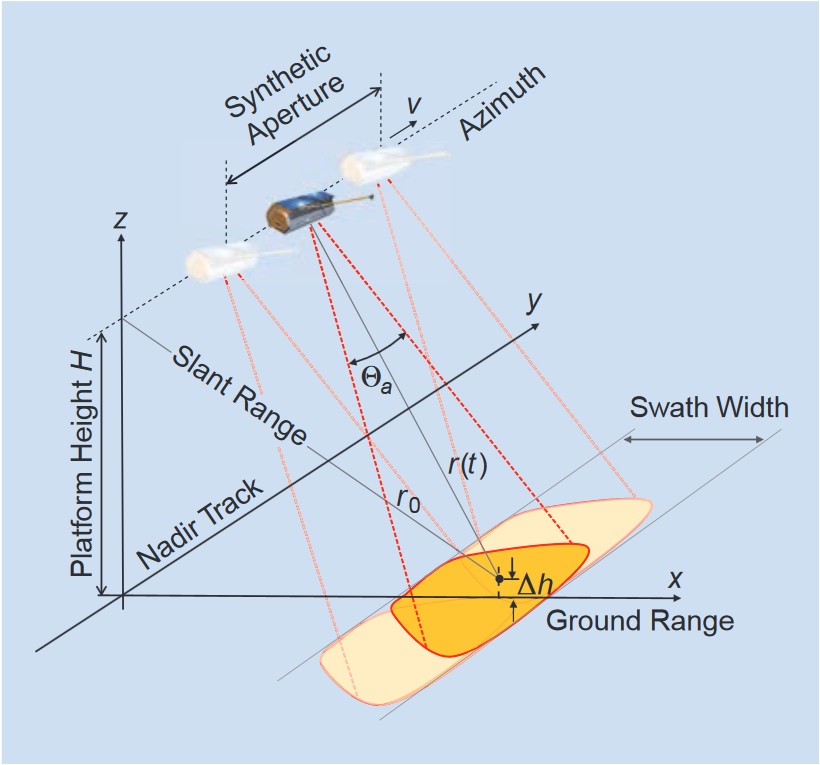
\includegraphics[width=0.8\linewidth]{Cap1/geometry.png}
    \caption{Illustration of SAR geometry. $r_0$ is the shortest distance to target, $\theta_a$ stands for the azimuth beam width and $v$ for the satellite speed. \cite{tutorial}}
    \label{fig:SAR_geometry}
\end{figure}{}

The resolution of an image in a given direction is the minimal distance between two points so it is still possible to identify the two different points on the image (also called to resolve the two different targets). In SAR there are resolution on range direction and azimuth direction, which is the minimal distance to separate two targets on range direction and azimuth direction respectively.\\
For resolving two separate targets, it is normally considered that the spatial separation of the pulses should be higher than half of the Bandwidth of the pulse (this is visually explained in \figref{fig:pulse_separation}).

\begin{figure}[H]
    \centering
    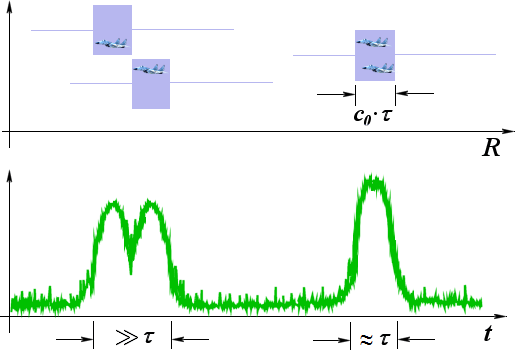
\includegraphics[width=0.8\linewidth]{Cap1/ra1_print.png}
    \caption{Temporal separation of pulses for target resolution. $\tau$ is the pulse temporal width}
    \label{fig:pulse_separation}
\end{figure}{}

From \figref{fig:pulse_separation}, it is possible to understand why it was adopted that the temporal separation should be greater than half $\tau$. If it is greater it's reasonable to assume that it is possible to separate the targets, but if it is less than that then it's not clear the target separation.

For SAR systems, the resolution in azimuth is equal to half the antenna length. And the resolution in range direction is given by: 

\begin{equation}
    \rho_{rg} = \frac{c\tau_{rg}}{2} = \frac{c}{2B_{rg}}
\end{equation}
where $\rho_{rg}$ is the range resolution, $c$ is the speed of the light, $\tau_{rg}$ is the temporal resolution and $B_{rg}$ is the bandwidth.

After acquiring the image of the area, it is necessary to filter the image, so it is clearer for interpretation and information extraction. This is done by using two matched filters (to maximize the signal-to-noise ratio of the image), one in the azimuth direction and the other in the range direction. 
This process of applying these two filters is called range compression and azimuth compression.

\figref{fig:sar_compression} gives a summary of how the azimuth and range compression works. The focusing process is done by making convolutions (usually carried out in frequency domain) with the reference function for the received signal in the range direction and in the azimuth direction.
\begin{figure}[H]
    \centering
    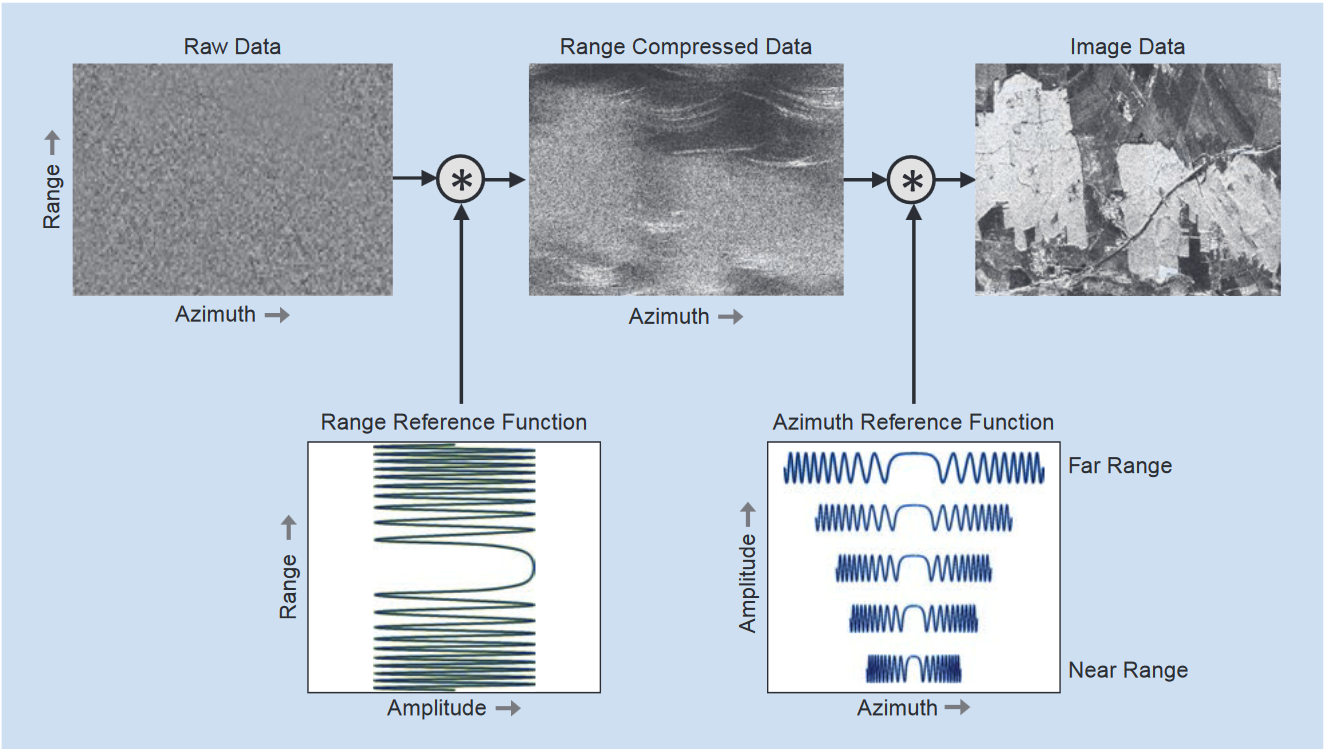
\includegraphics[width=\linewidth]{Cap1/compres.png}
    \caption{Summary of SAR compression in range and azimuth directions \cite{tutorial}}
    \label{fig:sar_compression}
\end{figure}

After the compression process it is finally obtained a complex matrix called Single Look Complex (SLC) matrix. The amplitude of each element of this SLC matrix represents the power reflected to the antenna. After the compression, it is possible to obtain the backscatter coefficient by multiplying the absolute value of the SLC by a calibration constant obtained experimentally.
The backscatter value acquisition is important because accurate backscatter values enable more accurate results in applications like deforestation monitoring, land-cover classification and delineation of wet snow covered area \cite{Small}. It is also important to mention that the local terrain has an important role in the determination of the backscatter value, and if a Digital Elevation Model (DEM) of the area is not available then the final result might be compromised.

According to \cite{Small} the radar backscatter $\beta$ is expressed as the ratio between scattered power $P_s$ and incident power $P_i$ at ground level: $\beta = \frac{P_s}{P_i}$. When one chooses a reference area $A_\beta$ in the slant range plane, it is possible to define the radar brightness or  $\beta^0$ backscatter according to \cite{Raney} as $\beta^0 = \frac{\beta}{A_\beta}$.

If the reference area is the ground area ($A_\sigma$), then the result is the \textit{sigma naught} and it is defined as $\sigma^0 = \frac{\beta^0 \cdot A_\beta}{A_\sigma} = \beta^0 \cdot \sin(\theta)$:


Instead, if the reference area is perpendicular to the line of sight $A_\gamma$, then the \textit{gamma naught} $\gamma^0$ is the result:

\begin{equation}
    \gamma^0 = \frac{\beta^0 \cdot A_\beta}{A_\theta} = \beta^0 \cdot \tan(\theta)
\end{equation}{}

A visual description of these normalized backscatter coefficients is shown in \figref{fig:normalization_areas}

\begin{figure}[H]
    \centering
    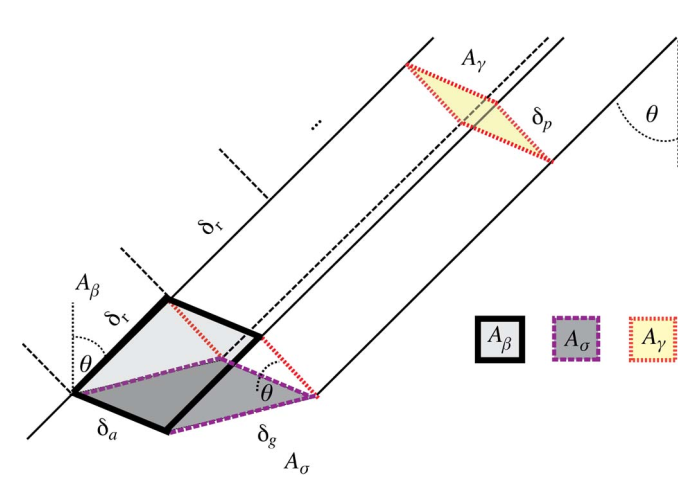
\includegraphics[width=0.8\linewidth]{Cap1/retang.png}
    \caption{Normalization areas for SAR backscatter \cite{Small}}
    \label{fig:normalization_areas}
\end{figure}


\subsection{SAR Image Geocoding}
\label{sec:sar_geocoding}

When an image of a SAR is acquired, there is no direct correspondence on the coordinates $(x,y,z)$ on the ground reference, since the coordinates of a pixel are in coordinates of range and azimuth. The process of transforming a SAR image from range and azimuth coordinates to local cartesian coordinates on the ground is called geocoding. By using the SAR image acquired, and a reference Digital Elevation Model of the area it is possible to find the points of the SAR image that correspond to the points of the Earth model used as a reference. It is important to make clear that it is absolutely necessary a DEM of the area since a SAR image is a 2D photo of a 3D area, and therefore it is not possible to make the inversion of coordinates since information is lost when making the image acquisition.

\section{SAR Interferometry}
\label{sec:sar_interferometry}
The SAR interferometry process uses the fact that two points on the ground with different heights when looked at two distinct positions in the plane perpendicular to the azimuth direction, will give a change in the phase difference of the received signal coming from these points.\\
By comparing acquisitions obtained at different antennas positions it is possible to extract additional information of a scene. The first time this was done was in 1974 by Graham \cite{Graham}, who obtained a pattern of interference fringes by vectorially adding the signals received from two SAR antennas.
One very important remark shown by \cite{Graham} is that the type of information extracted depends on the implementation of the system. If the images are acquired at different positions but at the same time, then it is possible to extract information about the topography of the area: this is called the across-track SAR interferometry (XTI-SAR). On the other hand, if the images are taken at different times it is possible to get a map of the surface velocities: this technique is called Differential InSAR(D-InSAR).


By taking the product of the first image with the conjugate of the second image it is possible to obtain the interferogram of that area. This interferogram is still not very useful for information extraction since there are more factors that affect the interferogram that must be compensated.
The first step important is the flat earth component removal of the interferogram, which is compensate the effect of the phase added to the interferogram due to the horizontal distance of the target. After the flat earth removal what is left is called the interferometric phase. \cite{Rosen} and \cite{Bamler} give a summary of how to compensate the flat earth component of the interferogram.


There are two kind of acquisitions that can be used for extracting inteferometric information.
\begin{itemize}
    \item 
    Repeat-pass interferometry: Where the images are acquired during different passes. Normally this means that there are a temporal interference and the quality is inferior, since it is subject to changes in the scene, atmospheric changes.
    \item
    Single-pass interferometry: Where the images are acquired at the same time. This means that the quality of the interferogram is superior, since there are less factors that can affect the final product. Since the temporal decorrelation does not affect this type of interferogram, it is chosen as the product for creation of a Digital Elevation Model (DEM) due to its superior quality.
\end{itemize}

\subsection{Height acquisition and interferogram equations}
Consider two SAR images acquired over the same area using sensors S1 and S2. The distance of the sensors is called the baseline $B$. Its projections, perpendicular and parallel to the slant range dimension, are the normal baseline $B_{\perp}$ and the parallel baseline $B_{\parallel}$, respectively. They are oriented at an angle $\beta$ with respect to the local horizontal.

\begin{figure}[H]
    \centering
    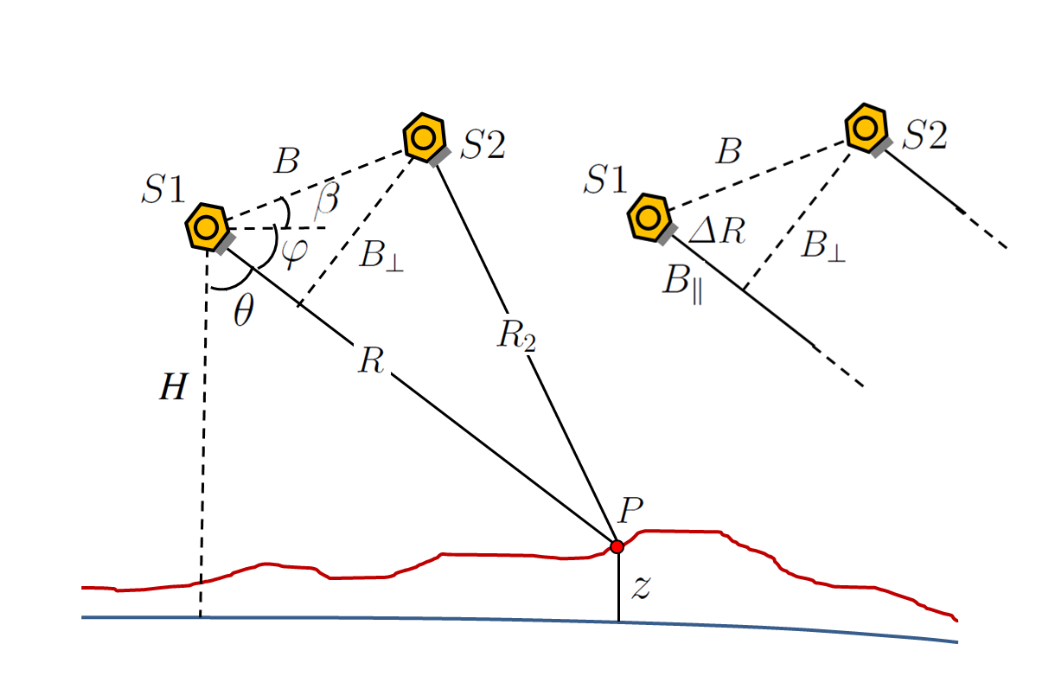
\includegraphics[width=\linewidth]{Cap1/int.png}
    \caption{Reference Geometry for Across-Track interferometry. \cite{Paolathesis}}
    \label{fig:reference_geometry}
\end{figure}

Since the slant-range distance is normally much greater than the baseline the following approximation holds true: $|R - R_2| \ll R$, where R is the distance from the Sensor S1 to the point on ground, R2 is the distance from sensor S2 to the point on ground.

The angle $\varphi$ is given by $\varphi = \frac{\pi}{2} - \theta$, 
and by applying the cossine law on triangle S1 S2 P it yields:
\begin{equation}
    (R-\Delta R) ^2 = R^2 + B^2 - 2BR \cos(\varphi + \beta)
\end{equation}

Using the parallel-ray aprroximation we get the following result:
\begin{equation}
    \Delta R = B \sin(\theta - \beta)
\end{equation}

And the topographical height $z$ is obteined as: 
\begin{equation}
    z = H - R\sin(\varphi)
\end{equation}
where $H$ is the height of S1.

By assuming a monostatic configuration (where both sensor acquire independently an image of the same area) we get 
finally that the phase of a pixel within the SAR image on sensor S1 is:
\begin{equation}
    \Phi_1 = -\frac{4\pi}{\lambda} R + \Phi_{obj,1}
\end{equation}
and the phase of a pixel within the SAR image on sensor S2 is:
\begin{equation}
    \Phi_2 = -\frac{4\pi}{\lambda} (R - \Delta R) + \Phi_{obj,2}
\end{equation}
where $\Phi_{obj,1}$ and $\Phi_{obj,2}$ are the phases in the images of Sensor S1 and S2. These phases in the images are assumed to be the same.

Therefore, the interferometric phase is obtained as the difference between the phases, such that:
\begin{equation}
    \Phi_{int} = \Phi_{1} - \Phi_{2} = -\frac{4 \pi}{\lambda} \Delta R
\end{equation}
and for a bistatic configuration (where only one radar transmits and both receive) it equals to:
\begin{equation}
    \Phi_{int} = -\frac{2 \pi}{\lambda} \Delta R
\end{equation}


Since the phase difference is half the phase difference for a bistatic configuration since the transmit path does not affect the phase difference.

The interferogram is the two dimensional image of the $\Phi_{int}$. It is worth mentioning that before the computation of the interferogram it is needed to make the coregistration of the images, that is merely to project one image on the geometry of the other image.
Once the interferogram has been computed the interferometric phase can be decomposed into two parts: the topographical phase component and the flat earth component.

\begin{equation}
    \Phi_{int} = \Phi_{topo} + \Phi_{fe}
\end{equation}
where $\Phi_{topo}$ is the topographic component and $\Phi_{fe}$ is the flat earth component.
The flat earth component accounts for the interferometric phase difference ocurring between two scatterers at the same topographical height but at different horizontal positions. The flat earth component is visually explained in \figref{fig:reference_geometry}.

\begin{figure}[H]
    \centering
    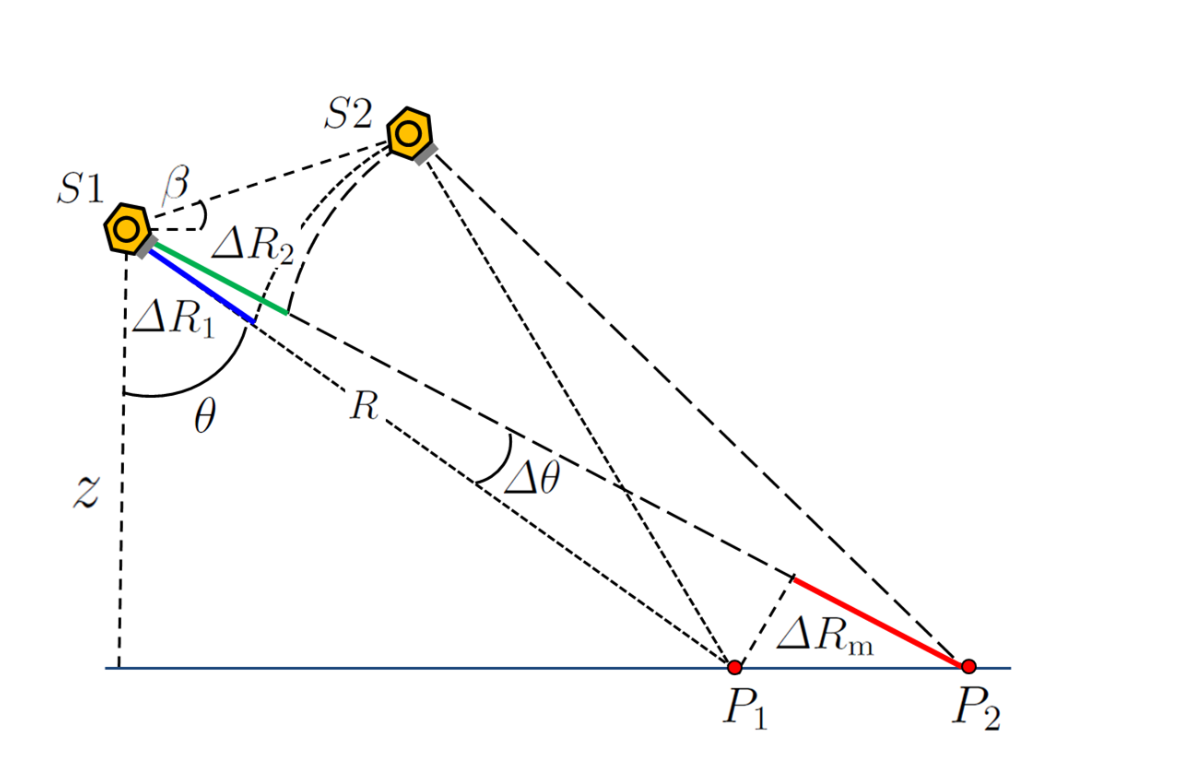
\includegraphics[width=\linewidth]{Cap1/flat.png}
    \caption{Reference Geometry for flat earth component. \cite{Paolathesis}}
    \label{fig:flat_earth_component}
\end{figure}

Consider now two points $P_1$ and $P_2$ on the same topographical height. The inteferometric phase for each one is given by:
\begin{equation}
    \Phi_1 = -\frac{4\pi}{\lambda}\Delta R_1 = -\frac{4\pi}{\lambda}B_{\perp}\sin(\theta - \beta)
\end{equation}
and for P2
\begin{equation}
    \Phi_2 = -\frac{4\pi}{\lambda}\Delta R_2 = -\frac{4\pi}{\lambda}B_{\perp}\sin(\theta + \Delta \theta - \beta)
\end{equation}

The difference between the two fases is the flat earth component that should be removed. Therefore the flat earth component equals to:
\begin{equation}
    \begin{aligned}
        \Phi_{fe} = & \Phi_1 - \Phi_2 = -\frac{4\pi}{\lambda}[B\sin(\theta + \Delta \theta - \beta) - B\sin(\theta - \beta)] = \\ 
        & \frac{4\pi}{\lambda}B\cos(\theta - \alpha)\Delta \theta
        \approx \frac{4\pi B\cos(\theta - \alpha)\Delta R_m}{\lambda R \tan(\theta)}
    \end{aligned}
\end{equation}
where $R_m$ is the slant range difference between $P1$ and $P2$.

The results of the extraction of the flat earth component can be visualized in the figure below.
\begin{figure}[H]
    \centering
    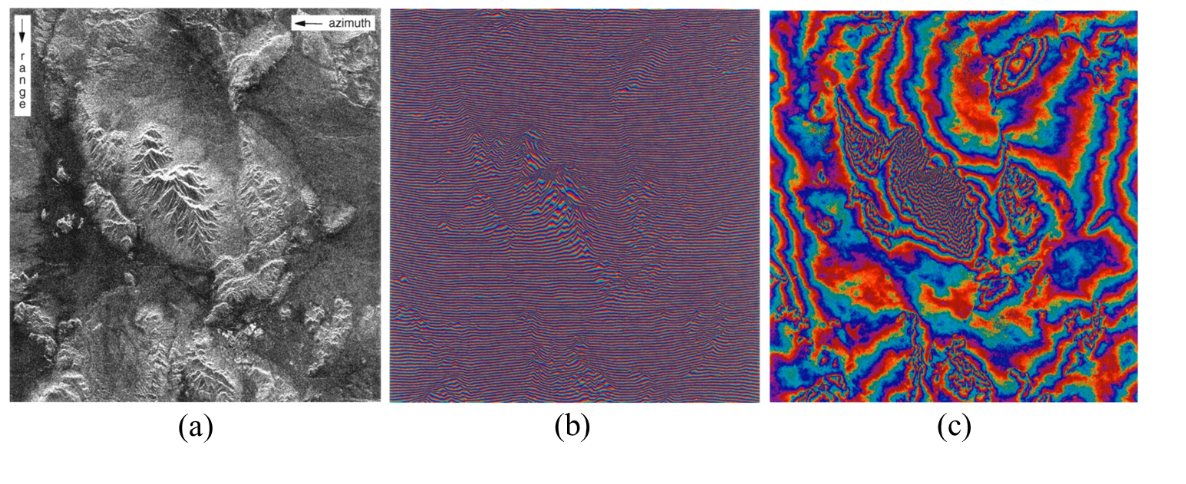
\includegraphics[width=\linewidth]{Cap1/flat_interf.png}
    \caption{(a) Amplitude of image of SAR image acquired by ERS-1/2 at C-Band with a baseline of $133$m.
    (b)Interferogram before the flat earth component removal. (c)Interferogram after the flat earth component removal. The color on the images represent the value of the interferometric phase of the pixel, such that pixels connected with the same color should have the same topographical height \cite{Paolathesis}}
    \label{fig:flat_earth_removal}
\end{figure}


The altitude difference $h_{amb}$ corresponding to a phase variation of $2\pi$ is called height of ambiguity. It is inversely proportional to the perpendicular baseline $B_{\perp}$ and is defined as:
\begin{equation}
    h_{amb} = \frac{\lambda R \sin(\theta)}{nB_{\perp}}
\end{equation}
where $n=2$ for monostatic configuration and $n=1$ for a bistatic configuration.
The idea is that the higher the perpendicular baseline the lower the height of ambiguity and therefore the more accurate the height estimation is.

It is also important to mention the process of phase unwrapping for the processing of the topographical phase component.\\
Since the topographical phase obtained is modulo $2\pi$ it is important to reconstruct the correct phase by adding multiples of $2\pi$ to the phase obtained. 
This process is called phase unwrapping and it is show in Figure 1.8.

\begin{figure}[H]
    \centering
    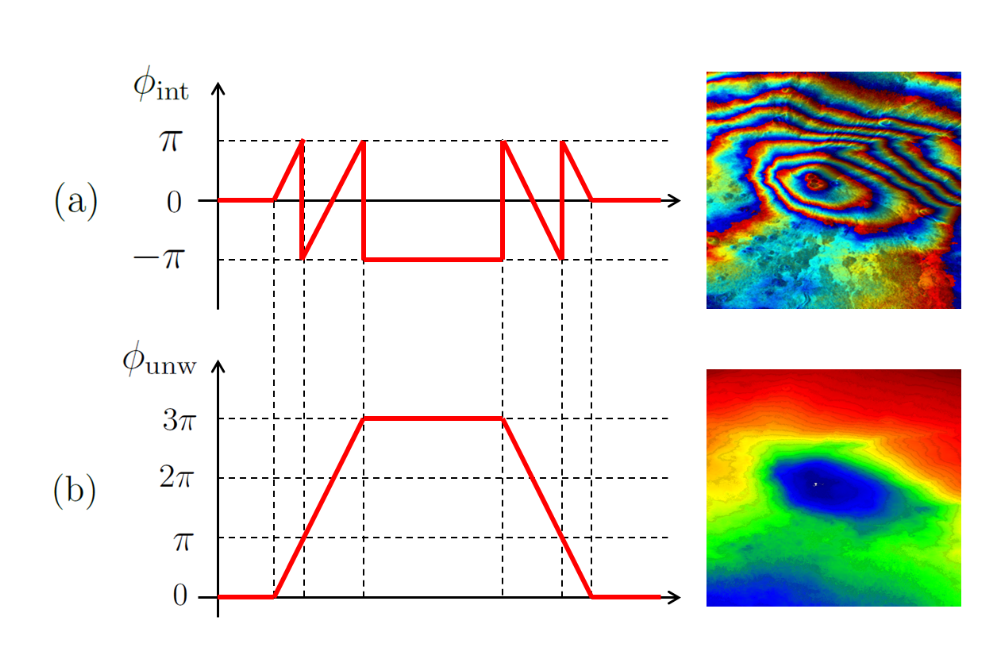
\includegraphics[width=\linewidth]{Cap1/unwr.png}
    \caption{Explanation about phase unwrapping. 
    (a) Topographical phase before the phase unwrapping.
    (b) Topographical phase after the unwrapping of the phase.
    The images are obtained from a repeat pass acquisition SIR-C-X SAR over Mount Etna, Italy. \cite{Paolathesis}}
    \label{fig:phase_unwrapping_process}
\end{figure}

After the flat earth removal and phase unwrapping the interferogram is finally ready for analysis and information extraction.

\subsection{The Complex Interferometric Coherence}
The interferometric coherence($\gamma_t)$ is a measure of the quality of the interferogram. It is, for each pair of corresponding pixels, the correlation between these two pixels: $u_1$ and $u_2$. It is given by:
\begin{equation}
    \rho = \frac{E[u_1u_2^*]}{\sqrt{E[|u_1|^2]E[|u_2|^2]}}
\end{equation}{}
where $E[\cdot]$ is the expectation operator. In practice it is not possible to obtain the correlation between the random variables that model the complex value of the pixels, so in practice this correlation is obtained by a moving average filter along the image.
What is obtained is then a estimation of the real value of the coherence, by using this moving average filter what is obtained is the Maximum Likelihood Estimation of the coherence. This is obtained as:
\begin{equation}
    \rho_{MLE}[i,j] = \frac{\sum_{i=1}^N[u_1[i]u_2^*[i]]}
    {\sqrt{\sum_{i=1}^N|u_1[i]|^2\sum_{i=1}^N|u_2[i]|^2}}
\end{equation}{}
Where $N$ is the number of independent samples used to compute the coherence estimation. 
The absolute value of the coherence, gives information about the decorrelation level and it is also a measure of the quality of the interferogram. The phase of the coherence, also called interpherometric phase, gives information about the path difference between the two antennas used for the acquisition. 

It is important to say that this estimation of the coherence is not unbiased, even though it is asymptotically unbiased \cite{Bamler}. In fact, if the values of the pixels are assumed to follow a gaussian distribution, then it is possible to find the relationship between the estimated coherence, the real value of the coherence and the number of samples used to make the estimation. This function is show in \figref{fig:bias}.

\begin{figure}[H]
    \centering
    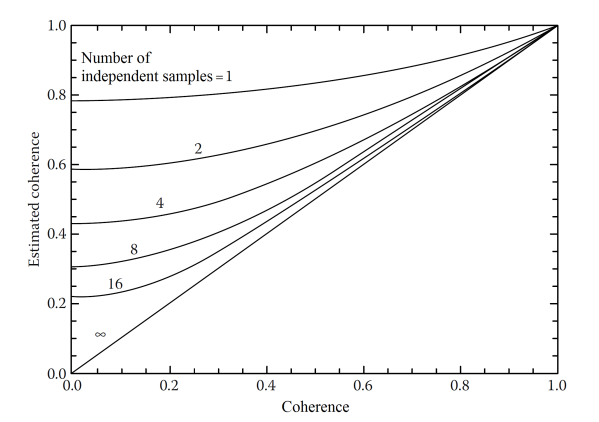
\includegraphics[width=\linewidth]{Cap1/bias.png}
    \caption{Bias of the MLE coherence estimator \cite{Bamler}.}
    \label{fig:bias}
\end{figure}

It is important to notice that the estimator is always biased towards higher values than it actually is, and by increasing the number of samples the estimation gets every time closer to the real value. It is also important to notice that for high values of the coherence the estimator provides a better estimation than it would if the coherence were of low value. 

This coherence number is crucial to the textures work that will be developed on the rest of the work, since there is much useful information for classification that can be extracted by looking at this number and by making the textures of the coherence image.

\subsection{Co-registration}
Before taking the complex interferometric coherence between the images, a step called co-registration is necessary. After making the focusing step of the two images, it is necessary to transform the slave image to what it would look like if it was taken with the acquisition geometry of the master image. Since the images are taken with different geometries, it produces effects of rototranslations that can scale differences between the images and induce errors in the coherence process. Therefore, this co-registration is a process that correctly alligns the two images to the same geometry and reduces the effects of errors in the calculation of the interferometric coherence\cite{andreathesis}.

\subsection{Decorrelation in Vegetated Areas}
According to \cite{Martone} different factors contribute to the total coherence and the coherence can be written as a product of the different contributions to the coherence as follows:

\begin{equation}
    \rho =\rho_{SNR}\cdot\rho_{Quant}\cdot\rho_{Amb}\cdot\rho_{Range}\cdot\rho_{Azimuth}\cdot\rho_{Vol}\cdot\rho{Temp}
\end{equation}

The terms on the right hand side describe the errors contribution due to: limited Signal to noise ratio ($\rho_{SNR}$), quantization errors($\rho_{Quant}$), ambiguities($\rho_{Amb}$),
baseline decorrelation 
($\rho_{Range}$), errors due to relative shift of the doppler spectra 
($\rho_{Azimuth}$), and temporal decorrelation($\rho_{Temp}$). 

The term ($\rho_{Vol}$) is the volume correlation factor and it is due to volume scattering. On forests this is mainly due to vegetation and therefore is crucial for forest land-cover classification.\\

A more detailed explanation about each contribution to the coherence is given by \cite{Martone2} and \cite{Rizzoli}, but a summary of each contribution is given following:

\begin{itemize}
    \item
    $\rho_{SNR}$: Is the coherence loss due to finite sensitivity of the radar system. It can be calculated from the Signal to Noise Ratio of the SAR System as follows:
    \begin{equation}
        \rho_{SNR}=\frac{SNR}{1+SNR}
    \end{equation}{}
    According to \cite{Martone3} for the TANDEM-X satellite system is holds that: \newline
    $\rho_{SNR}>0.8$
    \item
    $\rho_{Quant}$: It represents the error due to quantization of the recorded received signal. From \cite{Martone2} it is expected that this value is lower than 10\%.
    \item
    $\rho_{Range}$: Possible baseline decorrelation effects are estimated by deriving a local slope map from orbit and elevation information.
    \item
    $\rho_{Temp}$: Is the decorrelation due to the temporal baseline between both acquisitions. On TANDEM-X, since both acquisitions are taken almost at the same time it holds that $\rho_{Temp}\approx 1$.
    \item
    Also according to \cite{Martone3} and \cite{Krieger} the contributions of $\rho_{Amb}$ and $\rho_{Azimuth}$ are very small (less than 2\%) and are solved in the TANDEM-X by adaptative selection of the azimuth processing bandwidth and total independent zero Doppler steering.
\end{itemize}

In \cite{Krieger} there is a more detailed explanation about the different correlation factors.


In \cite{Paolo} it was also shown that a study about the evolution of the temporal correlation of an area can also provide useful information for land-cover classification. The temporal decorrelation is modelled in \cite{Paolo} as:
\begin{equation}
    \rho_{Temp} = (1-\rho_{LT})e^{-(\frac{t}{\tau})^2} + \rho_{LT}
\end{equation}{}
where $\gamma_{LT}$ is the long term coherence, $t$ is the time and $\tau$ is the target decorrelation factor. The determination of these parameters also provide  important information that might help improve the land cover classification algorithms. The work developed in \cite{Paolo} is crucial for this thesis, since this thesis is strongly based on this work and it lays the foundation for an improvement of land cover classification that is proposed on the end of this work.




\chapter{Classification Maps generated with SAR Images}
\label{cap:requisitos}
The goal of land cover mapping is to make a classification of different areas the Earth's global surface. Since land cover classification has several economical/social applications, such as, monitoring and environmental planning, it is crucial that classification maps be generated with high accuracy.

Classification maps can be generated in two different ways: by field measuring or through remote sensing. Field measuring provides a high accuracy classification map but there is the obvious problem that it does not scale well to large cover areas, since it takes a lot of time, money and it is limited to areas that can be easily accessed. 

Because of these problems mentioned above, classification maps are normally generated by using remote sensing data. The GlobCover (European Space Agency GlobCover Portal) map is one example of a classification map that was generated using MERIS data.

Some of the different areas of interest can be classified as: Vegetated areas, artificial surfaces (human made surfaces like constructions, buildings, roads, houses, etc...), water bodies, permanent snow or ice, among others. Some of these classes can be subclassified among different classes, for example, vegetation can mean: irrigated croplands, deciduous forests, mosaic grassland among others. The GlobCover classification map, provided by the European Space Agency is used to perform classification (European Space Agency GlobCover Portal). The GlobCover is composed of 23 different classes, which can be seen in the figure below. 

\begin{figure}[H]
    \centering
    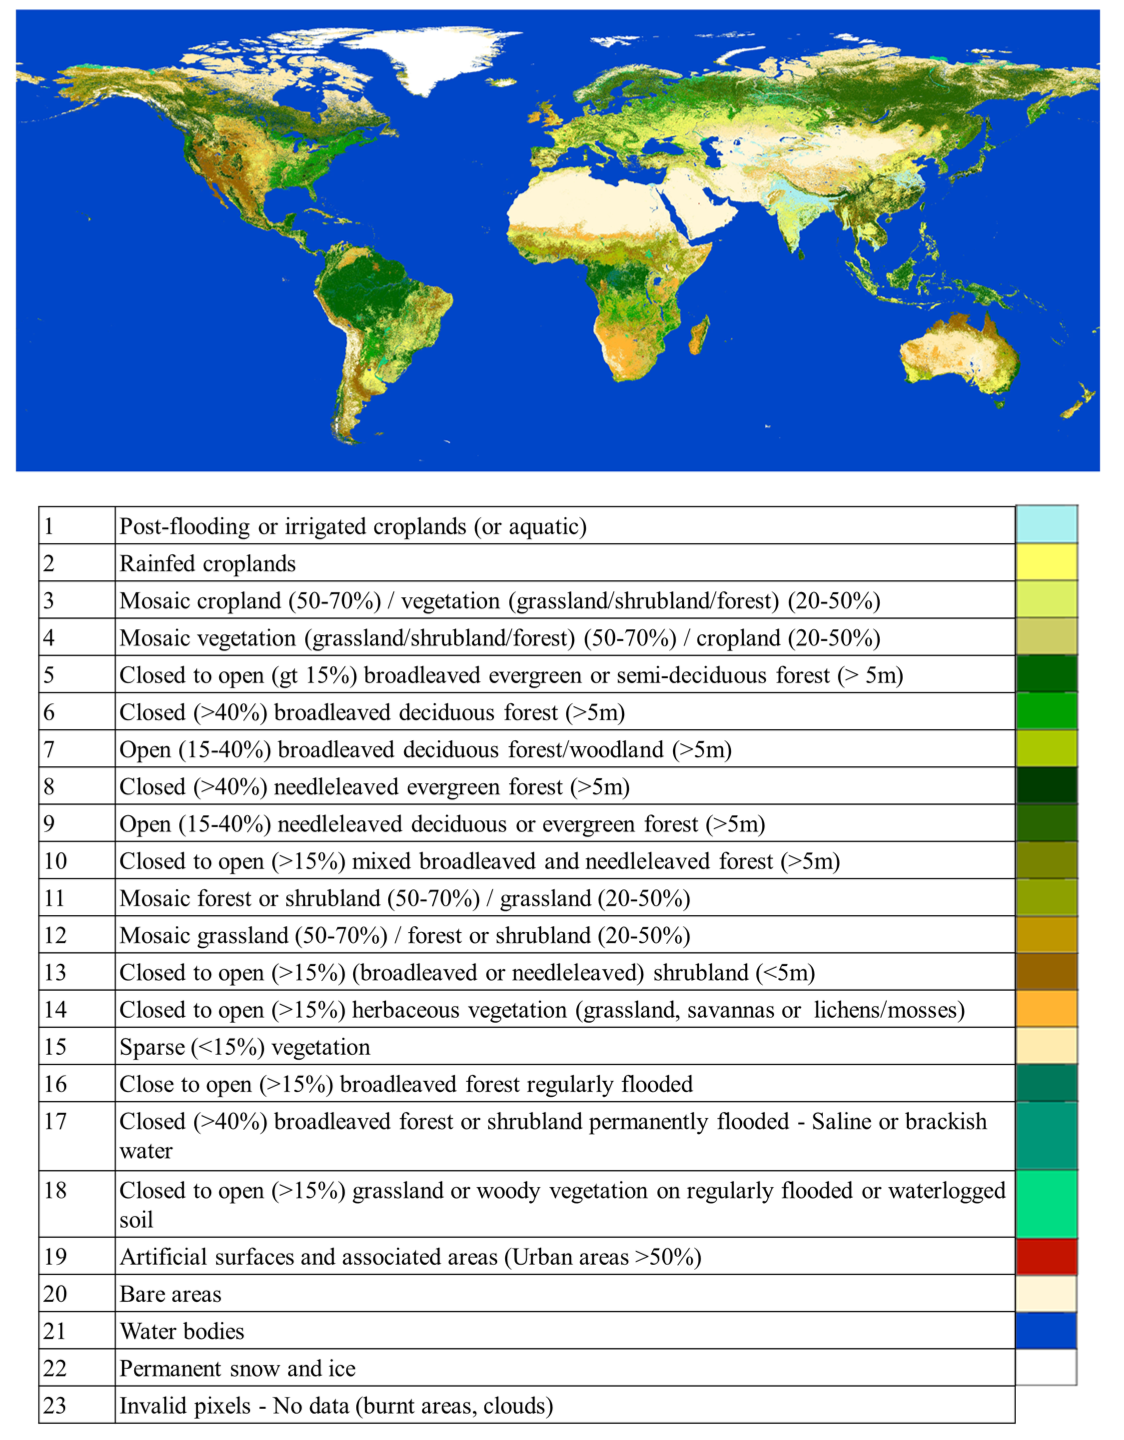
\includegraphics[width=\linewidth]{Cap2/glob_cover.png}
    \caption{GlobCover classification map.}
    \label{fig:glob_cover_map}
\end{figure}

Among the different classes mentioned above forests are a class that plays a key role in Earth's ecosystem. Therefore it is very important to analise the deforestation or change in forest areas in order to assess the impact of the ecosystem. 

Nowadays, optical and lasers sensors are used for land cover classification and forest changes, each with its own advantages. For example, optical sensors provide an easy way to make classification, but it has the disadvantages that it is weather dependent and cannot provide a high resolution map. SAR mapping has none of these disadvantages but it is harder to make a accurate classification. Given the necessity to generate classification maps throughout the year, independent of cloud coverage, detected SAR backscatter is widely used for forest mapping \cite{Krieger}. 

Some of these maps are very successful in the task of making an accurate forest map, such as the gobal forest/nonforest map L-Band ALOS PALSAR which was generated creating a threshold on the cross-polarization levels of the detected backscatter. Even though it is possible to generate classification maps using the signature backscatter, this work will focus on the creation of said maps by analizing the interferometric coherence.

The first use of interferometric data for forest mapping is reported on \cite{first_interferometric}. This work was used using ERS-1 SAR data and not only proved that forests can be clearly discriminated from other land categories, but it also showed that it is possible to distinguish among different forests types. This first approach consisted of analyzing the different values for the mean and standard deviation of the coherence for different areas, and by verifying that these values are separated. This method is visually explained in \figref{fig:first_interferometric_estimate}.

\begin{figure}[H]
    \centering
    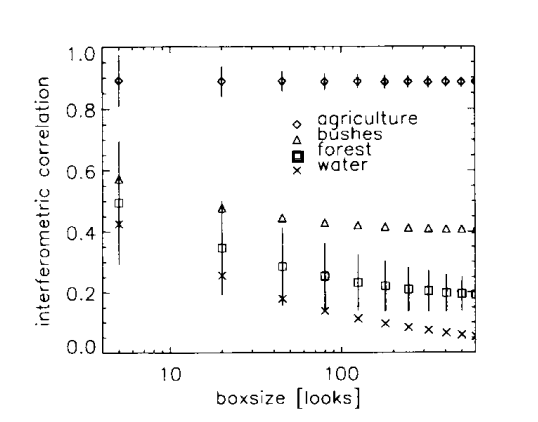
\includegraphics[width=0.7\linewidth]{Cap2/first_interferometric.png}
    \caption{Mean and Standard deviation of the coherence estimate as number of looks (filter size) for different classes.}
    \label{fig:first_interferometric_estimate}
\end{figure}

Nowadays, interferometric data can be used to monitor not only deforestation, but a series of other phenomena like topographical change and ice melting on polar caps \cite{Paolathesis}. 

On this work it will be presented the use of the ESA Sentinel-1 mission and its applications for forest mapping using the interferometric acquired data.

The Sentinel-1 mission consists of two sattelites which acquire data on a small temporal baselines (normally between 6 and 12 days) which use the C-band frequency range to acquire data in swaths of over 250km in range direction. Even though, like every SAR, the main product is the backscatter received from the target, the focus of this work is to rely only on the interferometric information for classification purposes. 

Some works rely on acquiring the backscatter data over large periods of time (months or years), and then classifying the target area based on the temporal change of it \cite{long_time_series}, this method is named long-time-series classification. Since the coherence is subjected to more variation over small periods of time, it is possible to make a classification based on its value, which don't have to be acquired over months, but over a few weeks is enough, this is why this method is called short-time-series classification, and since it has the capability of generate more updated maps, it was chosen as the method for this analysis. 

On this work it will be demonstrated that the short time series interferometric information is valuable resource for classification. Besides using the temporal model for classification, the result will also be combined with state of the art machine learning algorithms in order to even more improve the accuracy of the result obtained. 



\chapter{Material}
\label{cap:material rondonia}



\section{Test Area: The Rondonia State}
\par
The test area chosen for this thesis is the Amazon Rainforest, focusing specifically in the Rondonia state area. Rondonia topography is composed mainly by flat lands, which also have a lot of rivers thoroughout them, but also has regions of plateau with low altitude. The climate in Rondonia is what is called "humid equatorial" climate, which means that the temperature variation thorough the year is very little, something positive, since it is preferable to have no variations in the scene between SAR acquisition. The pluviometric indexes in the state can reach up to 2100mm per year, with most of the rains happening between May and September. The vegetation in the state (the focus of this thesis), just like most of north of Brazil, is the Amazon Rainforest, even though in some areas the \textit{Cerrado} vegetation is more common. The \textit{Cerrado} area is known for a very humid season and a very dry season, when the trees lose their leaves as a form of adaptation.
\par
The goal of this thesis is to improve algorithms to identify deforestation areas using SAR images. Because of that the natural choice of area to study was the Rondonia state, since it is the state with the most deforestation in the Amazon Rainforest. The Rondonia state already lost over 31\% of its forests and most of the remaining areas are degraded. For comparison, Acre, the state which borders Rondonia on the west, has 91\% of its original forest cover and a greater part of it is still intact. 
\par
Even though there are a lot of efforts being made to control the illegal deforestation, the results are not yet satisfactory and recent data even shows that the pace of deforestation have increased in the years of 2018 and 2019.\par
The deforestation in the Rondonia state can be easily seen with optical satellite data acquired with Google Earth. Deforestation follows a fairly predictable pattern, as seen in \figref{fig:fishbone}. The pattern of deforestation is known as fishbone pattern due to its similarity with a fish skeleton. This pattern arises from the fact that deforesting is normally done by penetrating the forest and then deforesting along the edges of the road firstly created.

\begin{figure}[H]
    \centering
    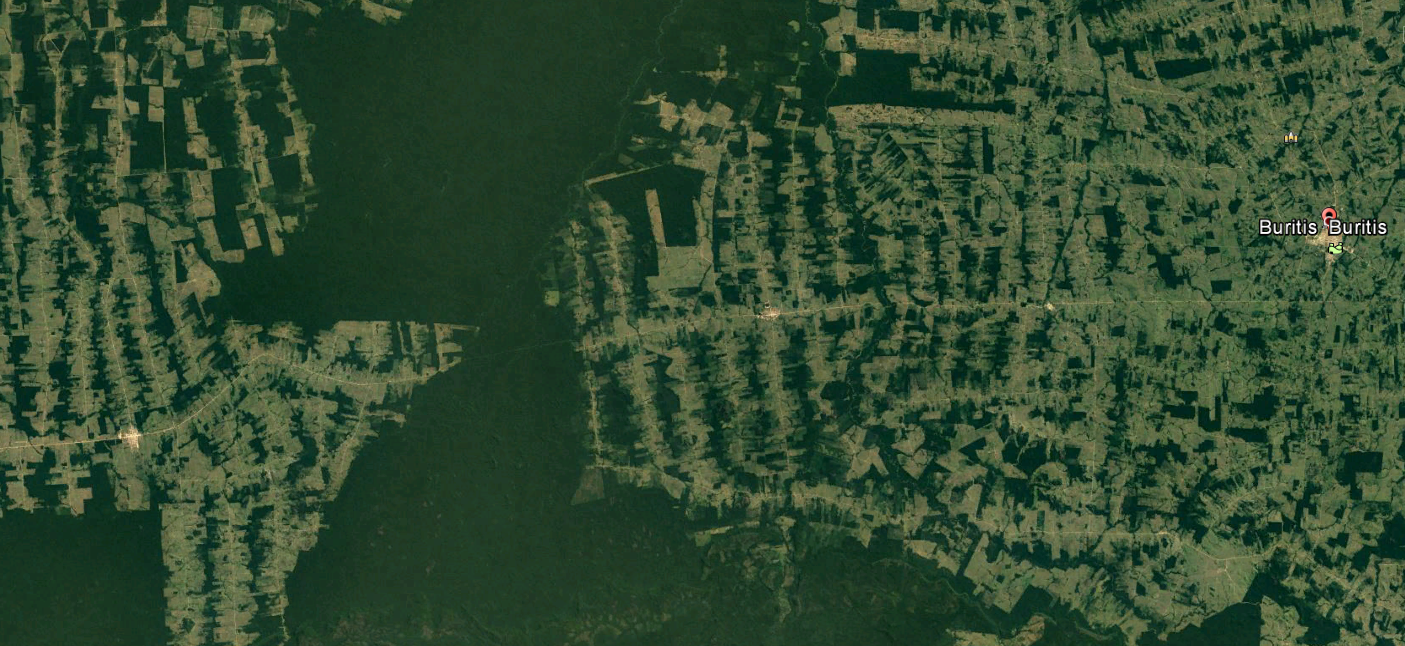
\includegraphics[width=0.8\linewidth]{Chapter2-real/fishbone.png}
    \caption{Fishbone pattern of deforestation(Image provided by Google Earth). }
    \label{fig:fishbone}
\end{figure}{}

Due to recent fires that happened in the year of 2019 in the Amazon Rainforest, there is much concern about studying and monitoring the deforestation that happens in that area, and considering that the Rondonia state is the area in which the deforestation is most critical, it was a natural choice of area to study for this thesis. 

\section{TanDEM-X datasets}
TerraSAR-X (TSX) and TanDEM-X (TDX), launched in June 2007 and June 2010, respectively, are two German SAR satellites operating in X-band, developed within a public/private partnership
between the German Aerospace Center (DLR) and Airbus Defence and Space. 


The goal of both satellites is to provide SAR products for commercial purposes and scientific purposes, and the TanDEM-X mission has the primary goal of generatin a global, high precision, and consistent digital elevation model (DEM) with full coverage and no gaps. The relevance of the mission lies in that, until now, the available DEMs
of large parts of Earth are of low resolution, inconsistent, incomplete and commonly
based on different data sources and survey methods.\newline TanDEM-X has offered, for the first
time, a global, high accuracy and homogeneous DEM. Besides the main goal, other secondary missions based on along-track interferometry have been defined as well
as new techniques with bistatic SAR \cite{vintetres, vintequatro}. The work presented on this thesis is one of the possible exploitation of the activities of the TanDEM-X data.

\begin{figure}[H]
    \centering
    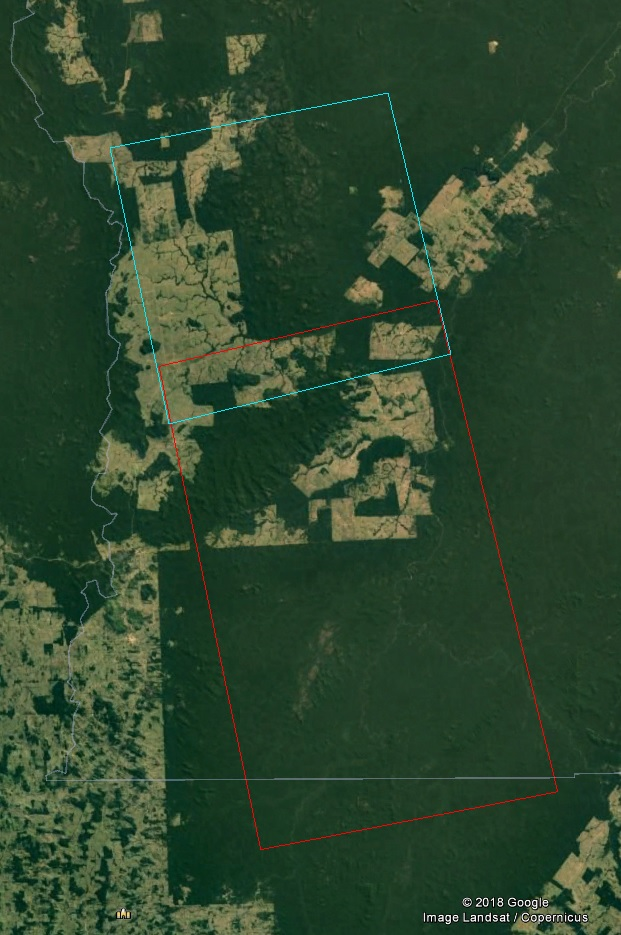
\includegraphics[width=0.6\linewidth]{Chapter2-real/tandem_dataset.jpg}
    \caption{TanDEM-X dataset available in Rondonia Area (Image provided by Google Earth).}
    \label{fig:tandem_dataset}
\end{figure}{}
TanDEM-X has the advantage that it can provide very high resolution data (each pixel has dimensions of  1.5m X 1.5m). Since the data is very resolution, and therefore very big in terms of memory size, it was chosen to work with small areas in the Rondonia state.
The dataset available is on the east of the Rondonia State. It was collected images from two areas in east Rondonia as can be seen in \figref{fig:tandem_dataset}. Each rectangle represents one SAR image acquired with the TanDEM-X.

\section{Sentinel-1 datasets}
\par
The SENTINEL-1 mission is a joint initiative of the European Commission (EC) and the European Space Agency (ESA). Copernicus, previously known as GMES, is a European initiative for the implementation of information services dealing with environment and security. It is based on observation data received from Earth Observation satellites and ground-based information.

Sentinel-1 is an imaging radar mission operating in C-band consisting of a constellation of two satellites aimed at providing day and night supply of imagery for users, independent of the weather at the time.
It also provides dual polarisation capability, very short revisit times and rapid product delivery. 
The constellation of two satellites, SENTINEL-1A and SENTINEL-1B, shares the same orbital plane.
\par
According to \cite{sentinelmission} there are five priorities for the SENTINEL-1 mission: To monitor sea ice zones and the arctic environment, surveillance of marine environment, to monitor land surface motion risks, mapping of land surfaces and mapping in support of humanitarian aid in crisis situations.

\begin{figure}[H]
    \centering
    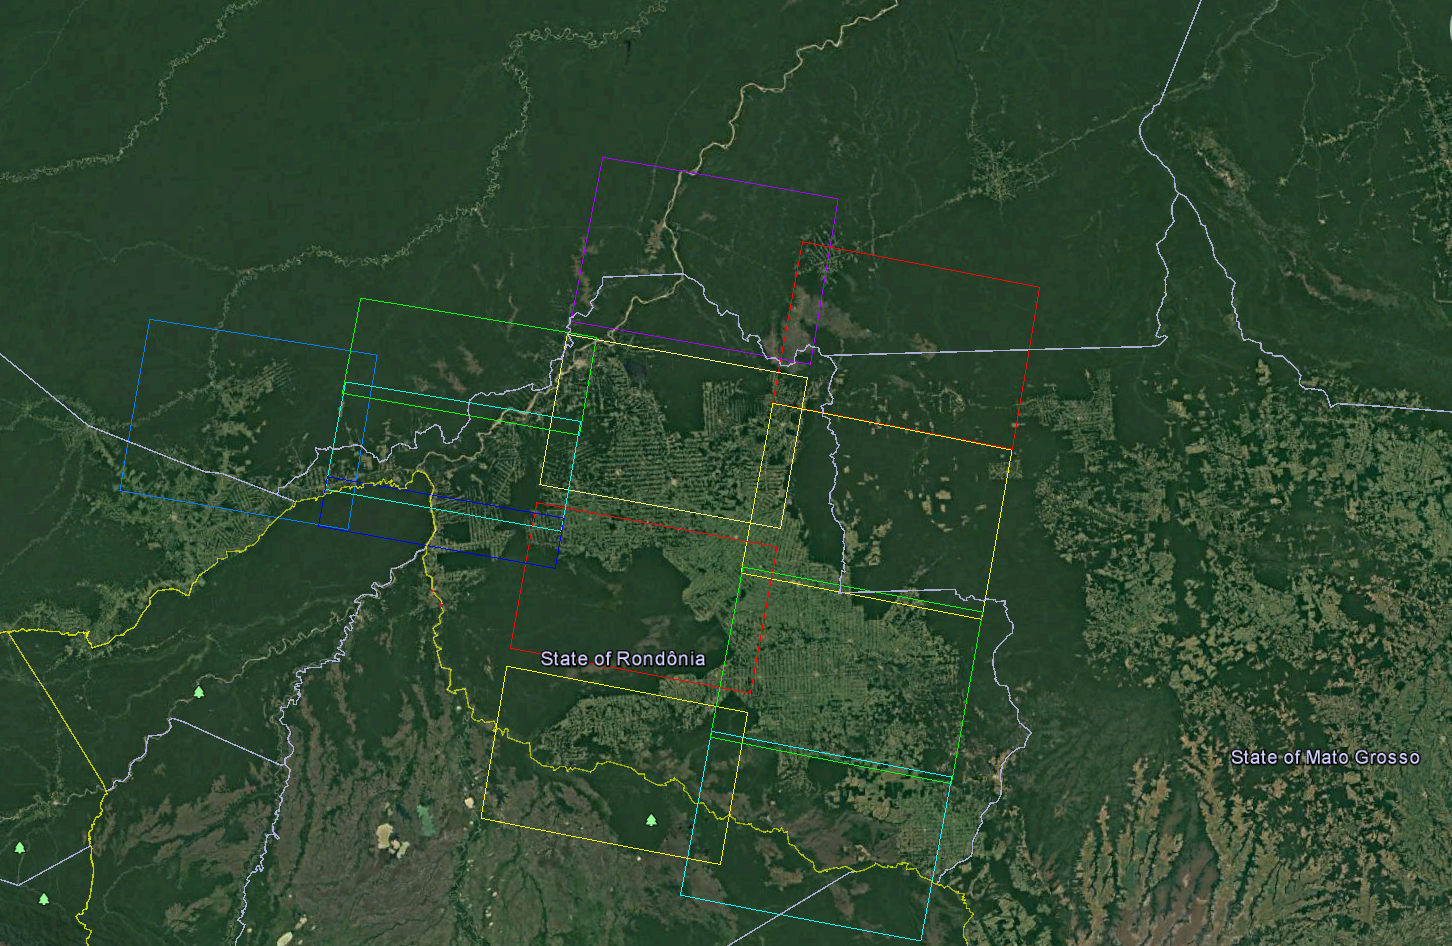
\includegraphics[width=\linewidth]{Chapter2-real/sentinel_dataset.png}
    \caption{SENTINEL-1 dataset available in Rondonia Area (Image provided by Google Earth).}
    \label{fig:sentinel_dataset}
\end{figure}{}

SENTINEL-1 provides area coverage much greater than the TanDEM-X satellite with coverage up to 400km, but the resolution of the image is lower compared to the TanDEM-X mission. While the pixel resolution for SENTINEL-1 mission is 3.7mX14m, the TanDEM-X can provide pixels with resolution of 1.5mX1.5m. Since SENTINEL-1 provides area coverage much greater than TanDEM-X, it was chosen as main option for area monitoring in the Rondonia state as a whole. With SENTINEL-1 it was possible to cover almost the entire Rondonia state although the entire coverage was not done because there are some gaps between acquisitions as seen on \figref{fig:sentinel_dataset}. Even though the resolution for the SENTINEL-1 is much lower than the resolution of the TanDEM-X, it will be investigated on this thesis if this resolution is enough to detect new areas of deforestation. The SENTINEL-1 dataset for the Rondonia state can be seen on \figref{fig:sentinel_dataset}, where each rectangle is one acquistion made by SENTINEL-1.

\chapter{Textures Methods for Image Analysis}
\label{cap:texture_methods}
%%%%%%%%%%%%%%%%%%%%%%%%%%%%%%%%%%%%%%%%%%%%%%%%%%%%%%%%%%%%%%%%%%%%%%%%%%%%%%%%
%2345678901234567890123456789012345678901234567890123456789012345678901234567890
%        1         2         3         4         5         6         7         8
% THESIS CHAPTER

% short summary of the chapter
\section*{Summary}
\label{sec:Summary_chap_2}
The objective of this work is to find techniques that might help improve classification and segmentation of SAR images.\newline
Given an image of the radar brightness ($\sigma^0)$ of an area or the image of the coherence between two SAR acquisitions it is possible to segment the image into different areas of interest, for example, given an image of the Amazon Forest someone might be interested in generating a map of the area that was deforested and the area that it is still preserved. \newline
Even though there are many machine-learning algorithms that can do this with an acceptable accuracy, these algorithms are not perfect and have a error that is noticeable. \newline
To improve the result of those algorithms the textures of the image will be analyzed and then it will be validated if it is possible to extract useful information from these textures that otherwise would be hidden to the traditional algorithms for classification, like random forest or neural networks.\newline
In some images, the texture might be a defining feature of a specific region and critical to obtain a correct classification.
The main idea of the looking at the textures of an image is to extract information based not only on the value of intensity of the pixel, but also looking at the pixels that are around that one, such that the value of a texture in a single pixel is a function that depends on the value of the original pixel and the pixels that are nearby it.\newline
The textures are a function of the spatial arrangement of intensities and colors in an image. Even though different images might have the same histograms of pixel intensities, they can be very different, and sometimes, analyzing just the histograms of the pixel intensities might not be enough to define in which region a pixel is in. There are two main approaches to analyze the textures of an image: the structural approach and the statistical approach. In this work it will be only used the statistical approach for analyzing textures.

\section{Machine Learning and the problems for classification}
\label{sec:machine_learning_problems}
Machine Learning is one of the most important and influential technologies in today's world. It is also one of the areas that has the most focus on research since the demand is very high, therefore it is very likely that there is still much room for improvement and its full potential has not yet been reached. \newline
Machine learning is a tool that was developed to deal with the excessive amount of data that has started to appear from 50 years ago until now. But this excessive amount of data is useless if there is no way to extract useful information from it. Focusing on this problem, machine learning is a field of study that tries to analyze data and find the hidden patterns hidden within it. Finding these patterns might be useful to make predictions of a problem and even help taking decisions on how to act when presented a situation.\newline
The name machine learning comes from the fact that the algorithms have to go through a learning process, trying different rules and seeing how well they perform to describe the problem presented. Among the different forms of machine learning, on this work there will be a focus on the supervised machine learning, which is a type of machine learning system that is presented with data which is labeled, that means that each data has a correct label. The goal of this machine learning is that when presented with new data it is possible to predict in which label that data fits. \newline

The are five steps to this process: Data collection, data preparation, model fitting, model evaluation and parameter tuning.
\begin{enumerate}
    \item Data collection: Collect the data the algorithm will learn from (in this case it is the SAR image)
    \item Data preparation: Format the data into optimal format for the algorithm.
    \item Training: The stage in which the algorithm derives a model by fitting the output and the input using some method.
    \item Evaluation: Check how well the algorithm performs
    \item Parameter Tuning: Tune the parameters to improve performance
\end{enumerate}{}

The types of Supervised learning are two: Classification and regression.
\begin{enumerate}
    \item Classification: The output is a category, like a color, or in the case of a SAR image, if the pixel indicates a area of forest or a deforested area.
    \item Regression: The output is a real number, such as height or price.
\end{enumerate}{}

On this work, classification machine learning will be used to classify a SAR image into regions of forest and deforested areas. \newline
There are several machine learning algorithms, such as: C-support vector classifier, K-nearest neighbors classifier, multi-layer perceptron, Gaussian process classification, Radial-basis function kernel, Decision tree classifier, AdaBoost classifier, Random forest classifier, Gaussian Naive Bayes classifier, Quadratic discriminant analysis classifier and neural network classifier.\newline

All those different algorithms try to solve the same problem: given a set of input labeled data, what is the model that best fits the labeled input data and the given label, in order to predict labels for unlabeled data with least error?\newline
The difference between those algorithms is that the model that each one will find is different. Some algorithms, like the neural network, will try to derive a model using linear functions on the input data and trying to minimize the mean square error(MSE) between the predicted output and the label for example, as the decision trees for example will try to create a series of binary questions and by combining the answers of these questions will give the label of the input data.
\newline
Either way, the model of each algorithm can be geometrically understood by creating decision regions in a $R^n$ space ($n$ is the number of input variables), and by looking in which region a input is located, it is possible to give the output answer.
\newline
For example, if the number of input variables is 2, and different algorithms are run to classify labeled data between two colors (blue and red) the result can be seen in the figure below.

\begin{figure}[H]
    \centering
    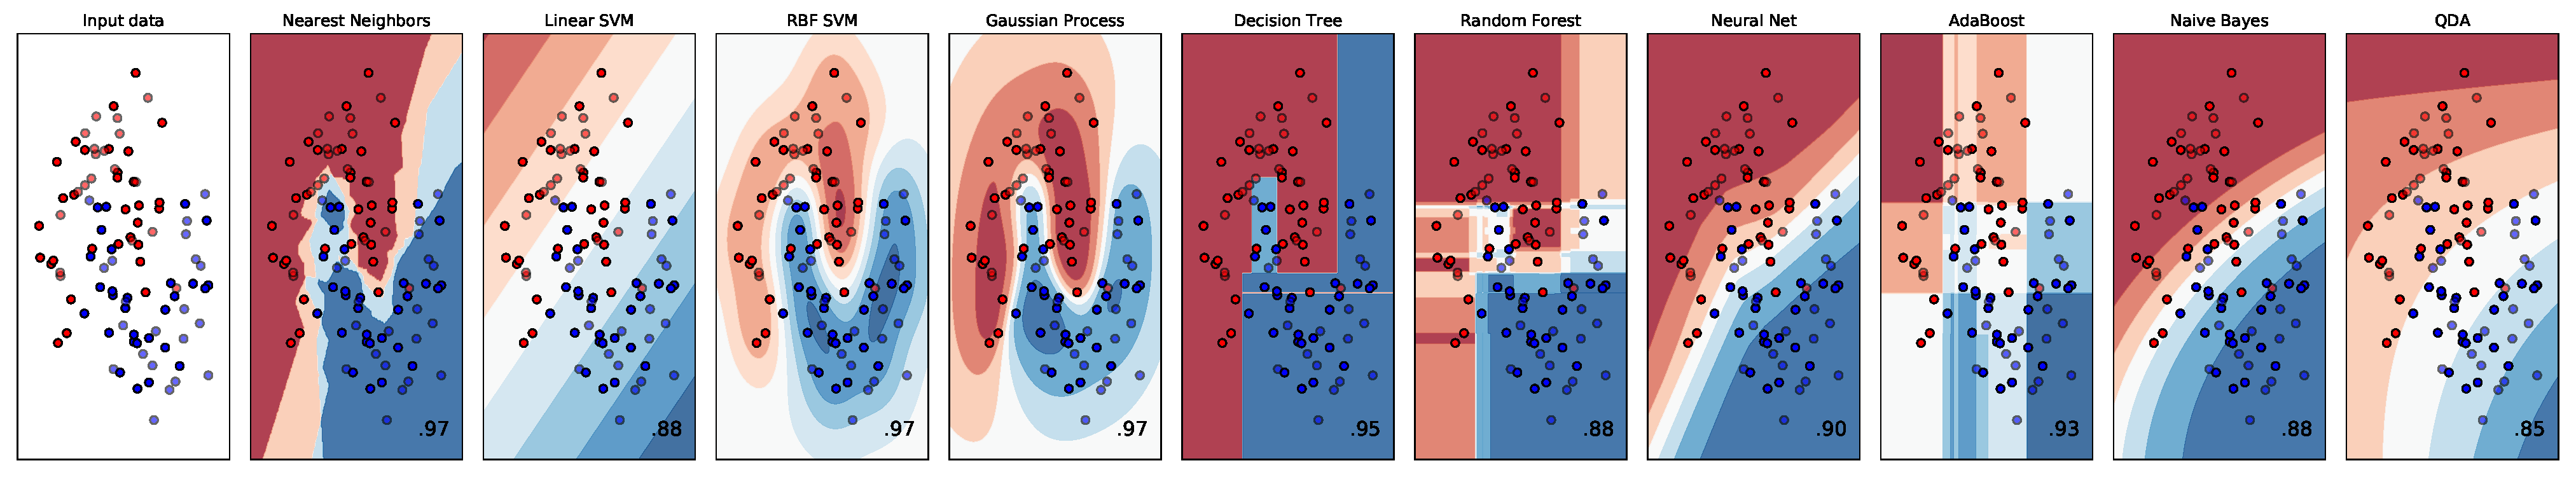
\includegraphics[width=\linewidth]{Chapter3/regions.pdf}
    \caption{Classification Boundaries for Different Algorithms}
    \label{fig:machine_learning_classification}
\end{figure}{}

In the image \ref{fig:machine_learning_classification} the color intensity illustrates how certain the algorithm is of the classification and the number on each figure is the time it took to create that region.
\newline
For different algorithms it is clear that the classification regions it derives are different and how the algorithm creates these regions determines how well the algorithm classifies.
\newline
The problem of using machine learning for classifying forest and deforested areas is that the algorithm relies too much on creating decision boundaries and by checking in which decision region a certain pixel is, but it does not check the surroundings of that pixel, which is also a important information for classification. \newline
\newline
For example, in the image \ref{fig:machine_learning_classification} above, if a red pixel falls in a blue region it will be wrongly labeled blue. For a SAR image it might happen that due to noise a forest pixel looks like a deforested pixel, but if all the pixels around it looks like forest pixels then this might be an indicator that that pixel is a wrongly labeled forest pixel. Even though it is not possible to make these machine learning algorithms consider this question in the learning process (this would mean interfering  in the modelling process, which would be equivalent to creating a new algorithm), it is possible to create more input data by looking at the surroundings of a pixel. This new data information can help this algorithm not to make a wrong classification. This new input data is exactly the textures of a image.

\section{Textures Methods}
\label{sec:Texturization_Methods}
As previously mentioned, the textures might give useful information for classification because sometimes the neighborhood of a pixel also provides valuable information for the classification. In forest landscapes, for example, the texture value might depend on the size and distance between trees, such that in high-resolution images if two pixels fall in the same tree then they will have similar value, resulting in a small local variance of intensities, something that will be indicated by the texture value. According to \cite{Woodcock} if the resolution is increased to a size comparable to the size to of trees, then the local variance also increases, something noticeable in tropical forests with a high species diversity. Therefore is important to mention that the texture is dependent of the resolution of the image, and the texture of a high resolution image of an area might be different than a low resolution image of the same area.

On this work it will be used three different textures methods for improving classification results: the Grey level co-occurrence matrix(GLCM) method, the Laws textures method and the sum and different histograms methods.

\section{The GLCM Method}
\label{sec:GLCM_Method}

The first method of texture creation is the grey-level-co-occurrence matrix method.
A co-occurrence matrix is a matrix extracted from an image in which the values in the rows and columns of this matrix represent the set of possible grey scale values of the image. 
For example, the co-occurrence matrix $C$ is a matrix in which the elements represent the possible co-occurrence of values for the image $I$ given a spatial relationship on a set of possible values $V$. 
For example, given a image, the co-occurrence matrix $C$ indicates how many times the value $i$ co-occurs with the value $j$ given a spatial relationship. 
This spatial relationship is given by a displacement vector $d = (d_r, d_c)$ that dictates the distance of the pixels that one wants to analyze the co-occurrence of values.
A more mathematical way to express this matrix is given by the following definition:

\begin{equation}
    C_{d}(i,j) = \# \{(r,c) | I(r,c)=i\  \textit{and} \  I(r+d_r, c+d_c)=j \} 
\end{equation}

For example, if the grey scale image $I$ is equal to:

\begin{equation}
I=
    \begin{bmatrix}
    1&1&0&0\\
    1&1&0&0\\
    0&0&2&2\\
    0&0&2&2
    \end{bmatrix} 
\end{equation}{}


Then three co-occurrence matrices for different displacement vectors $d=(0,1)$, $d=(1,0)$ and $d=(1,1)$ are:
\begin{equation}
    C_{(0,1)}=
    \begin{bmatrix}
    4&0&2\\
    2&2&0\\
    0&0&2
    \end{bmatrix}
\end{equation}{}

\begin{equation}
C_{(1,0)}=
    \begin{bmatrix}
    4&0&2\\
    2&2&0\\
    0&0&2
    \end{bmatrix}
\end{equation}{}

\begin{equation}
C_{(1,1)}=
    \begin{bmatrix}
    2&0&2\\
    2&1&1\\
    0&0&1
    \end{bmatrix}
\end{equation}{}

In $C_{(0,1)}$ the position $(0,0)$ equals 4, which means that $j=0$ appears to the right of $i=0$ four times in the image. The position $(1,0)$ equals 2 because $j=0$ appears to the right of $i=1$ two times in the image. The position $(2,1)$ equals 0 because $j=1$ never appears to the right of $i=2$.

From this grey level co-occurrence matrix it is important to generate the \textit{normalized} grey level co-occurrence matrix $N_d$ given by:

\begin{equation}
\label{eq:normalized}
    N_d(i,j) = \frac{C_d(i,j)}{\sum_i\sum_j C_d(i,j)}
\end{equation}
Co-occurrence matrices capture the texture properties, but are not directly useful for further analysis, such as comparing different textures. To solve this problem, is possible to compute numeric features from this normalized co-occurrence matrix that might give useful information of the image that otherwise would be hidden for machine learning classification algorithms. These numeric features computed from the normalized co-occurrence matrix represent more compactly the textures of the image.
The following textures are features that can be obtained from normalized co-occurrence matrix:
\begin{table}[H]
\centering
\begin{tabular}{ |c |c |}
 \hline
 Contrast & $\sum_{i,j=0}^{N-1} i\frac{N_d(i,j)}{1+(i-j)^2}$\\ 
 Dissimilarity & $\sum_{i,j=0}^{N-1} i N_d(i,j)|i-j|$\\
 Homogeneity & $\sum_{i,j=0}^{N-1}\frac{N_d(i,j)}{1+|i-j|}$\\
 Angular\ Second\ Moment & $\sum_{i,j=0}^{N-1} i N_d(i,j)^2$\\
 Correlation & $\sum_{i,j=0}^{N-1}\frac{(i-\mu)(j-\mu)N_d(i,j)}{\sigma^2}$\\
 Energy & $\sum_{i,j=0}^{N-1}N_d(i,j)^2$\\
 Entropy & $ -\sum_{i,j=0}^{N-1}N_d(i,j)\log_2(N_d(i,j))$\\
 \hline
\end{tabular}
\caption{Formula for texture calculations for GLCM Method}
\label{table:glcm_calculations}
\end{table}

Where $\mu$ is the GLCM mean and $\sigma$ is the standard deviations of the GLCM given by:

\begin{equation}
    \mu=\sum_{i,j=0}^{N-1}iN_d(i,j)
\end{equation}
\begin{equation}
    \sigma^2=\sum_{i,j=0}^{N-1}N_d(i,j)(i-\mu)^2
\end{equation}

A question that rises from this method is how to choose the displacement vector $d=(d_r,d_c)$ such that the result is the best. A solution proposed by  \cite{Zucker} is to run a hypothesis test to check the displacement vector $d$ that most rejects the hypothesis that the pair of pixels separated by the displacement vector $d$ are independent, therefore accepting the hypothesis that this pair of pixels give the most information one of the another and are better suited to compute a texture feature.
The hypothesis test suggests  to run a $\chi^2$ statistical test to find the value $d$ that give the most information, that is, to maximize the value:
\begin{equation}
    \chi^2(d) = (\sum_i\sum_j \frac{N_d^2(i,j)}{\sum_jN_d(i,j)\sum_iN_i(i,j)} -1)
\end{equation}

\section{The Laws Textures}
\label{sec:Laws_Textures}

A different way to create textures is to use 2D filters to detect different kinds of textures. Laws developed a method to measure the amount of variation of the image on a fixed sized window. The method consists of making 16 different convolutions of the original image with convolution masks and use the result to compute the texture. The 16 different filters are obtained by taking the product of the following vectors.
\begin{align}
L5 (Level) = 
\begin{bmatrix}
1&4&6&4&1
\end{bmatrix}\\
E5 (Edge) = 
\begin{bmatrix}
-1&-2&0&2&1
\end{bmatrix}\\
R5 (Ripple) = 
\begin{bmatrix}
-1&0&2&0&-1
\end{bmatrix}\\
S5 (Spot) = 
\begin{bmatrix}
1&-4&6&-4&1
\end{bmatrix}
\end{align}

Then the 2D convolution masks are obtained by taking the product of these vectors. For example the R5S5 mask is computed as the product of R5 and S5 as following:
\begin{equation}
\begin{bmatrix}
-1\\0\\2\\0\\-1
\end{bmatrix}
\times
\begin{bmatrix}
1&-4&6&-4&1
\end{bmatrix}
=
\begin{bmatrix}
-1&0&2&0&-1\\
4&0&-8&0&4\\
-6&0&12&0&-6\\
4&0&-8&0&4\\
-1&0&2&0&-1
\end{bmatrix}
\end{equation}

After applying the 16 5x5 masks to the image it is necessary to generate the texture energy map on a fixed size window. Let the window size be 15x15 and $F_k[i,j]$ the result of the $kth$ mask on the pixel [i,j]. Then the texture energy map $E_k$ is defined by:
\begin{equation}
E_k[r,c] = \sum_{j=c-7}^{c+7}\sum_{i=r-7}^{r+7} |F_k[i,j]|   
\end{equation}

After creating the 16 energy maps it is needed to group together similar images that perceive the textures in different directions. For example, if R5S5 detects at ripples in the vertical direction, then S5R5 detects ripples in the horizontal direction, so it is desirable to group them together to detect ripple in both directions. The average of these two images measure then the total ripple content. It is possible to group the 16 energy maps in 9 texture images as following:
\begin{align*}
L5E5/E5L5\qquad L5S5/S5L5\\
L5R5/R5L5\qquad\qquad\ \ E5E5\\
E5S5/S5E5\qquad E5R5/R5E5\\
S5S5\qquad\qquad\ \ S5R5/R5S5\\
R5R5
\end{align*}


\section{The Sum and Difference Histograms Texture}
\label{sec:sum_and_diff_hist_texture}
\subsection{The Single Value Decomposition}
Let $I[k,l]$ be a discrete image which is the realization of a bi-dimensional stationary process and let $G=\{1, 2,...,N_g\}$ be the set of the $N_g$ quantized grey levels.
Just as in the GLCM method, consider a pair of pixels $y_1$ and $y_2$ separated by a displacement vector $d = (d_1, d_2)$ such that:
\begin{equation}
\begin{cases}
&y_1 = I[k,l]\\
&y_2 = I[k+d_1, l+d_2]
\end{cases}
\end{equation}
The discrete joint probability function of these two pixels is $P(y_1, y_2)$. And the probability of observing a pair of grey-level occurrence $i$ and $j$ separated by a displacement vector $(d_1, d_2)$ is given by:
\begin{equation}
    Prob\{y_1=i,\  y_2=j\} = P(i,j,d_1,d_2) = P(i,j)
\end{equation}
which does not depend on the pixel position $[k,l]$.

Pay attention to the fact that an estimate of this joint distribution $P[i,j]$ is the normalized co-occurrence matrix given by \ref{eq:normalized}, such that:
\begin{equation}
    \hat{P}(i,j) = N_d[i,j] \simeq P(i,j)
\end{equation}
\newline

Let us consider the random vector of the two random variables $y_1$ and $y_2$. Let $Y$ be this random vector such that $Y=[y_1, y_2]^T$. Suppose that this random vector $Y$ has a co-variance matrix $C_{yy}$. The goal is to make a linear transformation on this vector such that the new vector has uncorrelated variables. Suppose the linear transformation is given by a matrix $H$ and the new random vector is $Z$ such that:
\begin{equation}
    Z=HY
\end{equation}{}
It is known from \cite{papoulis} that the co-variance matrix $C_{zz}$ of the random variable $Z$ is obtained by the following formula.
\begin{equation}
    C_{zz} = HC_{yy}H^T
\end{equation}
If we make a single value decomposition on the matrix $C_{yy}$ such that $C_{yy} = U\Lambda^2U^T 
=U\Lambda \Lambda U^T$ and we choose the matrix $H$ such that $H = \Lambda^{-1}U^T$ then the co-variance of the random vector $Z$ is given by:
\begin{equation}
    C_{zz} = HC_{yy}H^T = \Lambda^{-1}U^T U\Lambda \Lambda U^T U \Lambda^{-1} = I
\end{equation}{}
Therefore the components of Z are uncorrelated.

Let us model the random vector $Y$ to have similar cross-correlation between the variables, such that:
\begin{equation}
    C_{yy} = \sigma_y^2 
    \begin{bmatrix}
    1&\rho\\
    \rho&1
    \end{bmatrix}
\end{equation}{}
where
\begin{equation}
    \sigma_y^2\ \rho = E\{(y_1-\mu)(y_2-\mu)\} \ and \ \mu = E\{y_1\} = E\{y_2\}
\end{equation}{}
And due to stationarity
\begin{equation}
    E\{(y_1-\mu)^2\}=E\{(y_2-\mu)^2\} = \sigma_y^2
\end{equation}{}

Let us make then the transformation given by
\begin{equation}
H =\frac{1}{\sqrt{2}} 
\begin{bmatrix}
1&1\\
1&-1
\end{bmatrix}{}
\end{equation}
That results in the new random vector $Z=[z_1, z_2]^T$ that:
\begin{equation}
\begin{cases}
&z_1 =\frac{y_1+y_2}{\sqrt{2}}\\
&z_2 = \frac{y_1-y_2}{\sqrt{2}}
\end{cases}
\end{equation}
Such that the new co-variance matrix for $Z$ is given by:
\begin{equation}
C_{zz}=
    \begin{bmatrix}
    \sigma_y^2 (1+\rho) & 0\\
    0 & \sigma_y^2 (1-\rho)
    \end{bmatrix}{}
\end{equation}{}

\subsection{Approximation of Probability Density Functions}
Let $\alpha \in N_g$ and $\beta \in N_g$.
If we assume that the variables for $y_1$ and $y_2$ are gaussian, then $z_1$ and $z_2$ are also gaussian and uncorrelated, therefore the joint probability function can be calculated from:

\begin{equation}
P(y_1=\alpha, y_2=\beta) = P(z_1=\alpha + \beta, z_2=\alpha - \beta) = P_s(z_1=\alpha+\beta)\cdot P_d(z_2=\alpha-\beta) 
\end{equation}

If the variables are not gaussian then the equality is not valid, but it is still a valid approximation to the probability function $P(y_1, y_2)$. 
\begin{equation}
    \hat{P}_y(i,j) = c_0\cdot P_s(i+j) \cdot P_d(i-j) \simeq P_y(i,j)
    \label{approximation_gaussian}
\end{equation}{}
Where $c_0$ is a normalization constant that assures that
\begin{equation}
    \sum_{i=1}^{N_g}\sum_{j=1}^{N_g} \hat{P}_y(i,j) = 1
\end{equation}{}

The relative error of this approximation can be computed analyzing the Kullback-Leibler Divergence between the two variables $P$ and $\hat{P}$ as follows
\begin{equation}
\label{eq:divergence}
    I(P, \hat{P}) = \sum_i\sum_j P_y(i,j)\cdot log(\frac{P_y(i,j)}{\hat{P}(i,j)}) = \\
    H_s + H_d - H_y -log(c_0)\geq0
\end{equation}{}
Where $H_s$, $H_d$ and $H_y$ are the entropies given by:
\begin{equation}
\begin{cases}
&H_y = -\sum_{i=1}^{N_g}\sum_{j=1}^{N_g}P_y(i,j)\cdot log(P_y(i,j)\\
&H_s = -\sum_{k=2}^{2N_g}P_s(k)\cdot log(P_s(k)\\
&H_d = -\sum_{l=-N_g+1}^{N_g-1}P_d(l)\cdot log(P_d(l))
\end{cases}
\end{equation}
This divergence is a measure of the error of approximating one distribution for another, and is equal to zero only when the two variables have the same distribution, therefore it will only be zero if $P(i,j)=\hat{P}(i,j)$. The importance of \ref{eq:divergence} is that it is possible to see the independence of the new variables by comparing only the entropy of the sum and difference to the entropy of the co-occurrence matrix. The closer the mutual information $I(P, \hat{P})$ is to zero, the better the approximation defined by \ref{approximation_gaussian}

\subsection{Textures Features}
It was shown that the sum and difference are a linear transformation that uncorrelates the random variables of the pair of the pixels. Therefore it is suggested by \cite{Unser} to replace the regular co-occurrence matrix by the associated histograms of the sum and difference estimated from the original image.
The non-normalized sum and difference associated with the displacement vector $d=(d_1,d_2)$ are given by:
\begin{equation}
\begin{cases}
&s_{k,l} = I[k,l] + I[k+d_1, l+d_2]\\
&d_{k,l} = I[k,l] - I[k+d_1, l+d_2]
\end{cases}
\end{equation}

And then we make the normalized histograms of these new vectors. The histograms of the sum and difference are given by:
\begin{equation}
\begin{cases}
&h_s(i, d_1, d_2) = h_s(i) = |\{(k,l) \in G, \ s_{k,l} = i\}|\\
&h_d(j, d_1, d_2) = h_d(j) = |\{(k,l) \in G, \ d_{k,l} = j\}|
\end{cases}
\end{equation}
And the normalized sum and difference histograms are given by:
\begin{equation}
\begin{cases}
&\hat{P}_s(i) = \frac{h_s(i)}{\sum_i h_s(i)} \qquad (i=2,...,2N_g)\\
&\hat{P}_d(i) = \frac{h_d(i)}{\sum_j h_d(i)} \qquad (j=-N_g+1, ... ,N_g-1)
\end{cases}
\end{equation}
And these normalized sum and difference histograms are estimates of the sum and difference probability functions given by:
\begin{equation}
\begin{cases}
&P_s(i) = Prob\  \{s_{k,l} = i\} \qquad (i=2,...,2N_g)\\
&P_d(j) = Prob\  \{d_{k,l} = j\} \qquad (j=-N_g+1, ... ,N_g-1)
\end{cases}
\end{equation}


From these estimates of the probability density functions it is possible to compute textures. There are 9 important textures that will be used through this work. On the table below there are the computation formulas for them:


\begin{table}[H]
\centering
\begin{tabular}{ |c |c |}
 \hline
 mean & $\frac{1}{2}\sum_i i\hat{P}_s(i)$\\ 
 variance & $\frac{1}{2}(\sum_i (i-2\mu)^2\hat{P}_s(i) + \sum_j (j)^2\hat{P}_d(j))$\\
 energy & $\sum_i \hat{P}_s(i)^2 \ \sum_j \hat{P}_d(j)^2$\\
 correlation & $\frac{1}{2}(\sum_i (i-2\mu)^2\hat{P}_s(i) - \sum_j (j)^2\hat{P}_d(j))$\\
 entropy & $-\sum_i\hat{P}_s(i)log_2(\hat{P}_s(i)) - \sum_j\hat{P}_d(j)log_2(\hat{P}_d(j))$\\
 contrast & $\sum_j j^2 \hat{P}_d(j)^2$\\
 homogeneity & $\sum_j\frac{1}{1+j^2} \hat{P}_d(j)$\\
 cluster shade & $\sum_i (i-2\mu)^3 \hat{P}_s(i)$\\
 cluster prominence & $\sum_i (i-2\mu)^4 \hat{P}_s(i)$\\
 \hline
\end{tabular}
\caption{Formula for texture calculations for Sum and Difference Histograms Method}
\label{table:sum_and_diff_calculations}
\end{table}


It is also important to know which size the window should be to compute the histograms for the sum and difference. Through this work the window size chosen was to be a regular window of size 10x10.
The number of gray levels is also important. Through this work, unless specified, the images will be normalized and scaled manually to have 10 different grey levels.
\\
Theoretically, if the variables were gaussians, then this method would give the same result as the Gray-Level Co-Occurrence matrix method, since if the variables are gaussians are uncorrelated then they are independent and the formula given by $(4.29)$ holds exactly and is not just and approximation. If they are not gaussians then the approximation is not perfect, but there is a great computational advantage to use this method, since making histograms of 1-D vectors is much faster than extracting a 2-D co-occurrence matrix. On the next section it will be analyzed if this method gives a nice result compared to the other 2 and if it is worth it to use this method due to the computational advantage.


\chapter{Analysis of Texture Results}
\label{cap:analysis_texture_results}
%%%%%%%%%%%%%%%%%%%%%%%%%%%%%%%%%%%%%%%%%%%%%%%%%%%%%%%%%%%%%%%%%%%%%%%%%%%%%%%%
%2345678901234567890123456789012345678901234567890123456789012345678901234567890
%        1         2         3         4         5         6         7         8
% THESIS CHAPTER

% short summary of the chapter
\section*{Summary}
On this section it will be demonstrated the results of different textures being applied to a SAR image and it will be analyzed which textures, if any, might help improve classification algorithms for forest areas and deforested areas. On this section it will be presented textures results of images of the coherence between 2 SAR images, and radar brightness ($\beta^0$)

\section{The GLCM Textures} 
\label{sec:gv1}

\subsection{The Displacement Vector}
\label{subsec:displacement_vector}
The first step to compute the textures of a image using the GLCM method is to choose the displacement vector $d=(d_1, d_2)$ that will be used to compute the grey level co-occurrence matrix. As said in the previous chapter, one way to choose this value is to use a statistical test proposed by \cite{Zucker} to find the value of $d$ that gives more texture information.
The process to compute to find the best $d$ consists of computing the grey level co-occurrence matrix for different displacement vectors and extracting the chi-squared statistical value for that occurrence matrix. The chi-square value is given by:
\begin{equation}
    \label{eq:test}
    \chi^2(d) = (\sum_i\sum_j \frac{N_d^2(i,j)}{\sum_jN_d(i,j)\sum_iN_i(i,j)} -1)
\end{equation}

It is expected that the closer the distance between the pixels the better, since pixels that are more close together in the image have bigger correlation between them. This statistical test will be run on coherence images over Amazon forest and $\beta^0$ images over Amazon forest to confirm that pixels that are closer have greater correlation between them.  
% \begin{figure}
%   \centering
%   \subfloat[]{
%     \label{fig:cap4_beta0}
%     \input{Chapter4/coSSC_master_beta0.png}
%   }
%   \subfloat[]{
%     \label{fig:cap5_gammavol}
%     \input{Chapter4/coSSC_master_gamma_vol.png}
%   }
% \end{figure}

\begin{figure}[H]
  \centering
    \begin{subfigure}[b]{0.4\linewidth}
      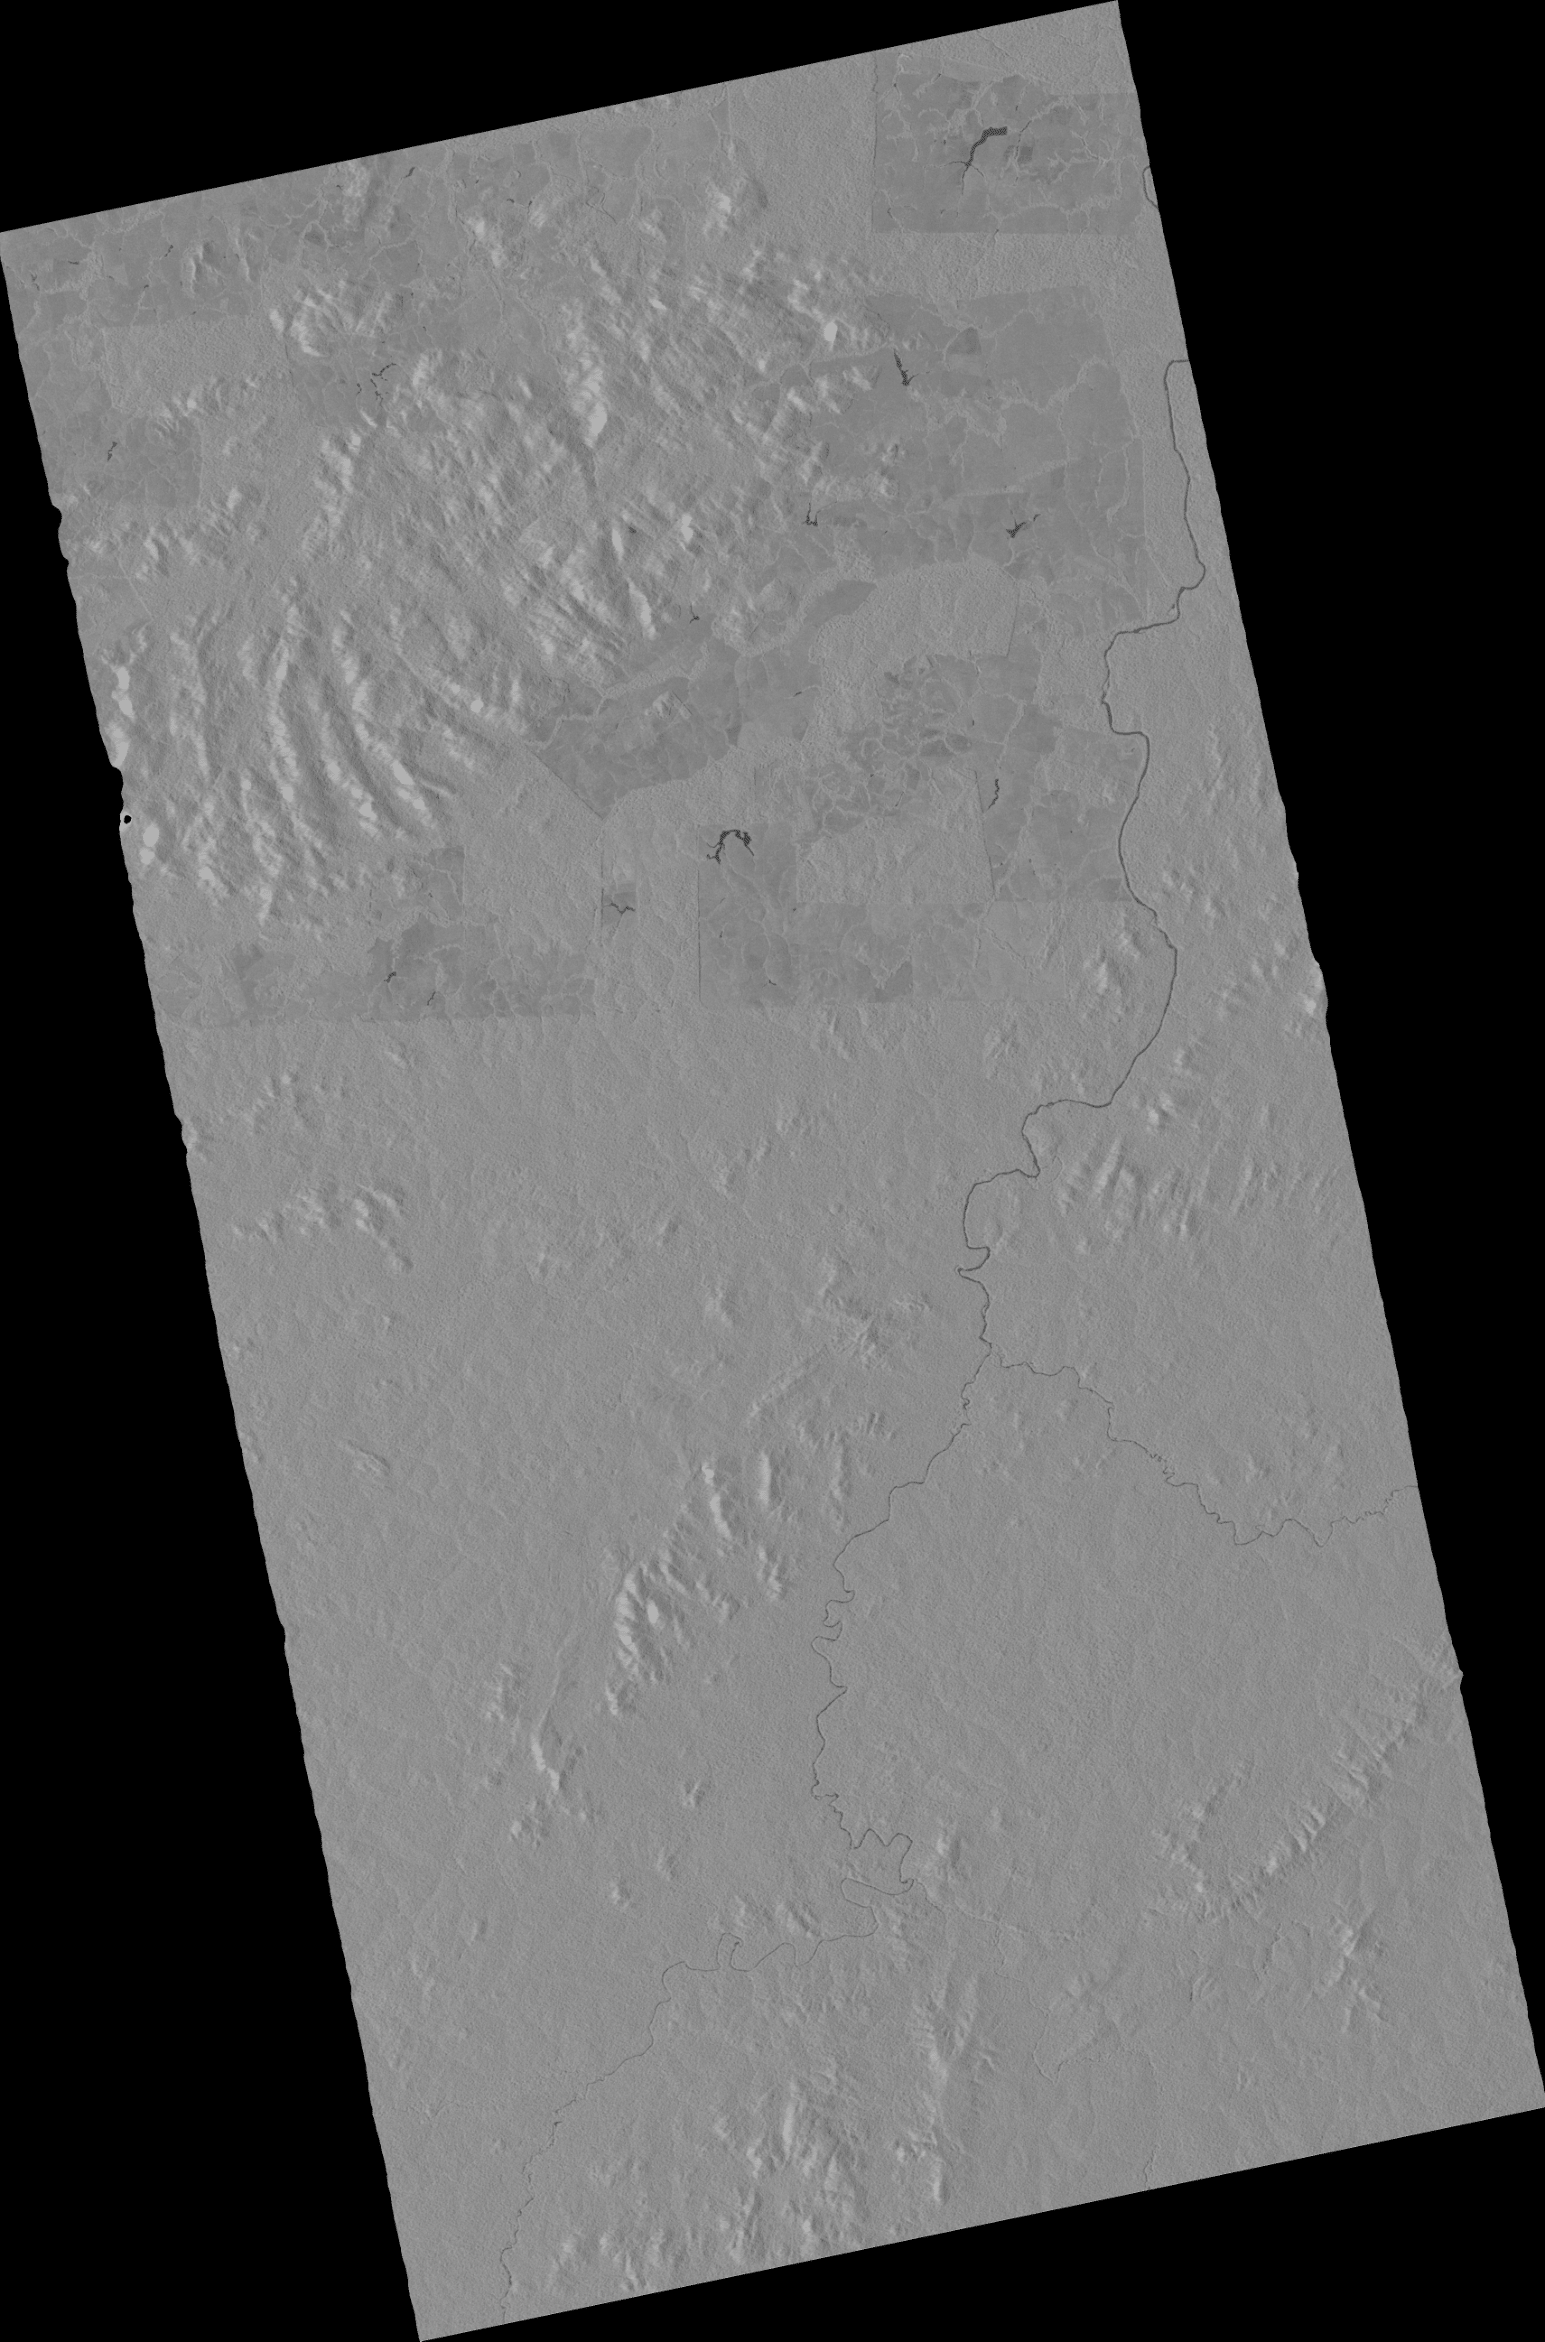
\includegraphics[width=0.8\linewidth]{Chapter4/coSSC_master_beta0.png}
      \caption{$\beta^0$ Image of Amazon area}
    \end{subfigure}
    \begin{subfigure}[b]{0.4\linewidth}
      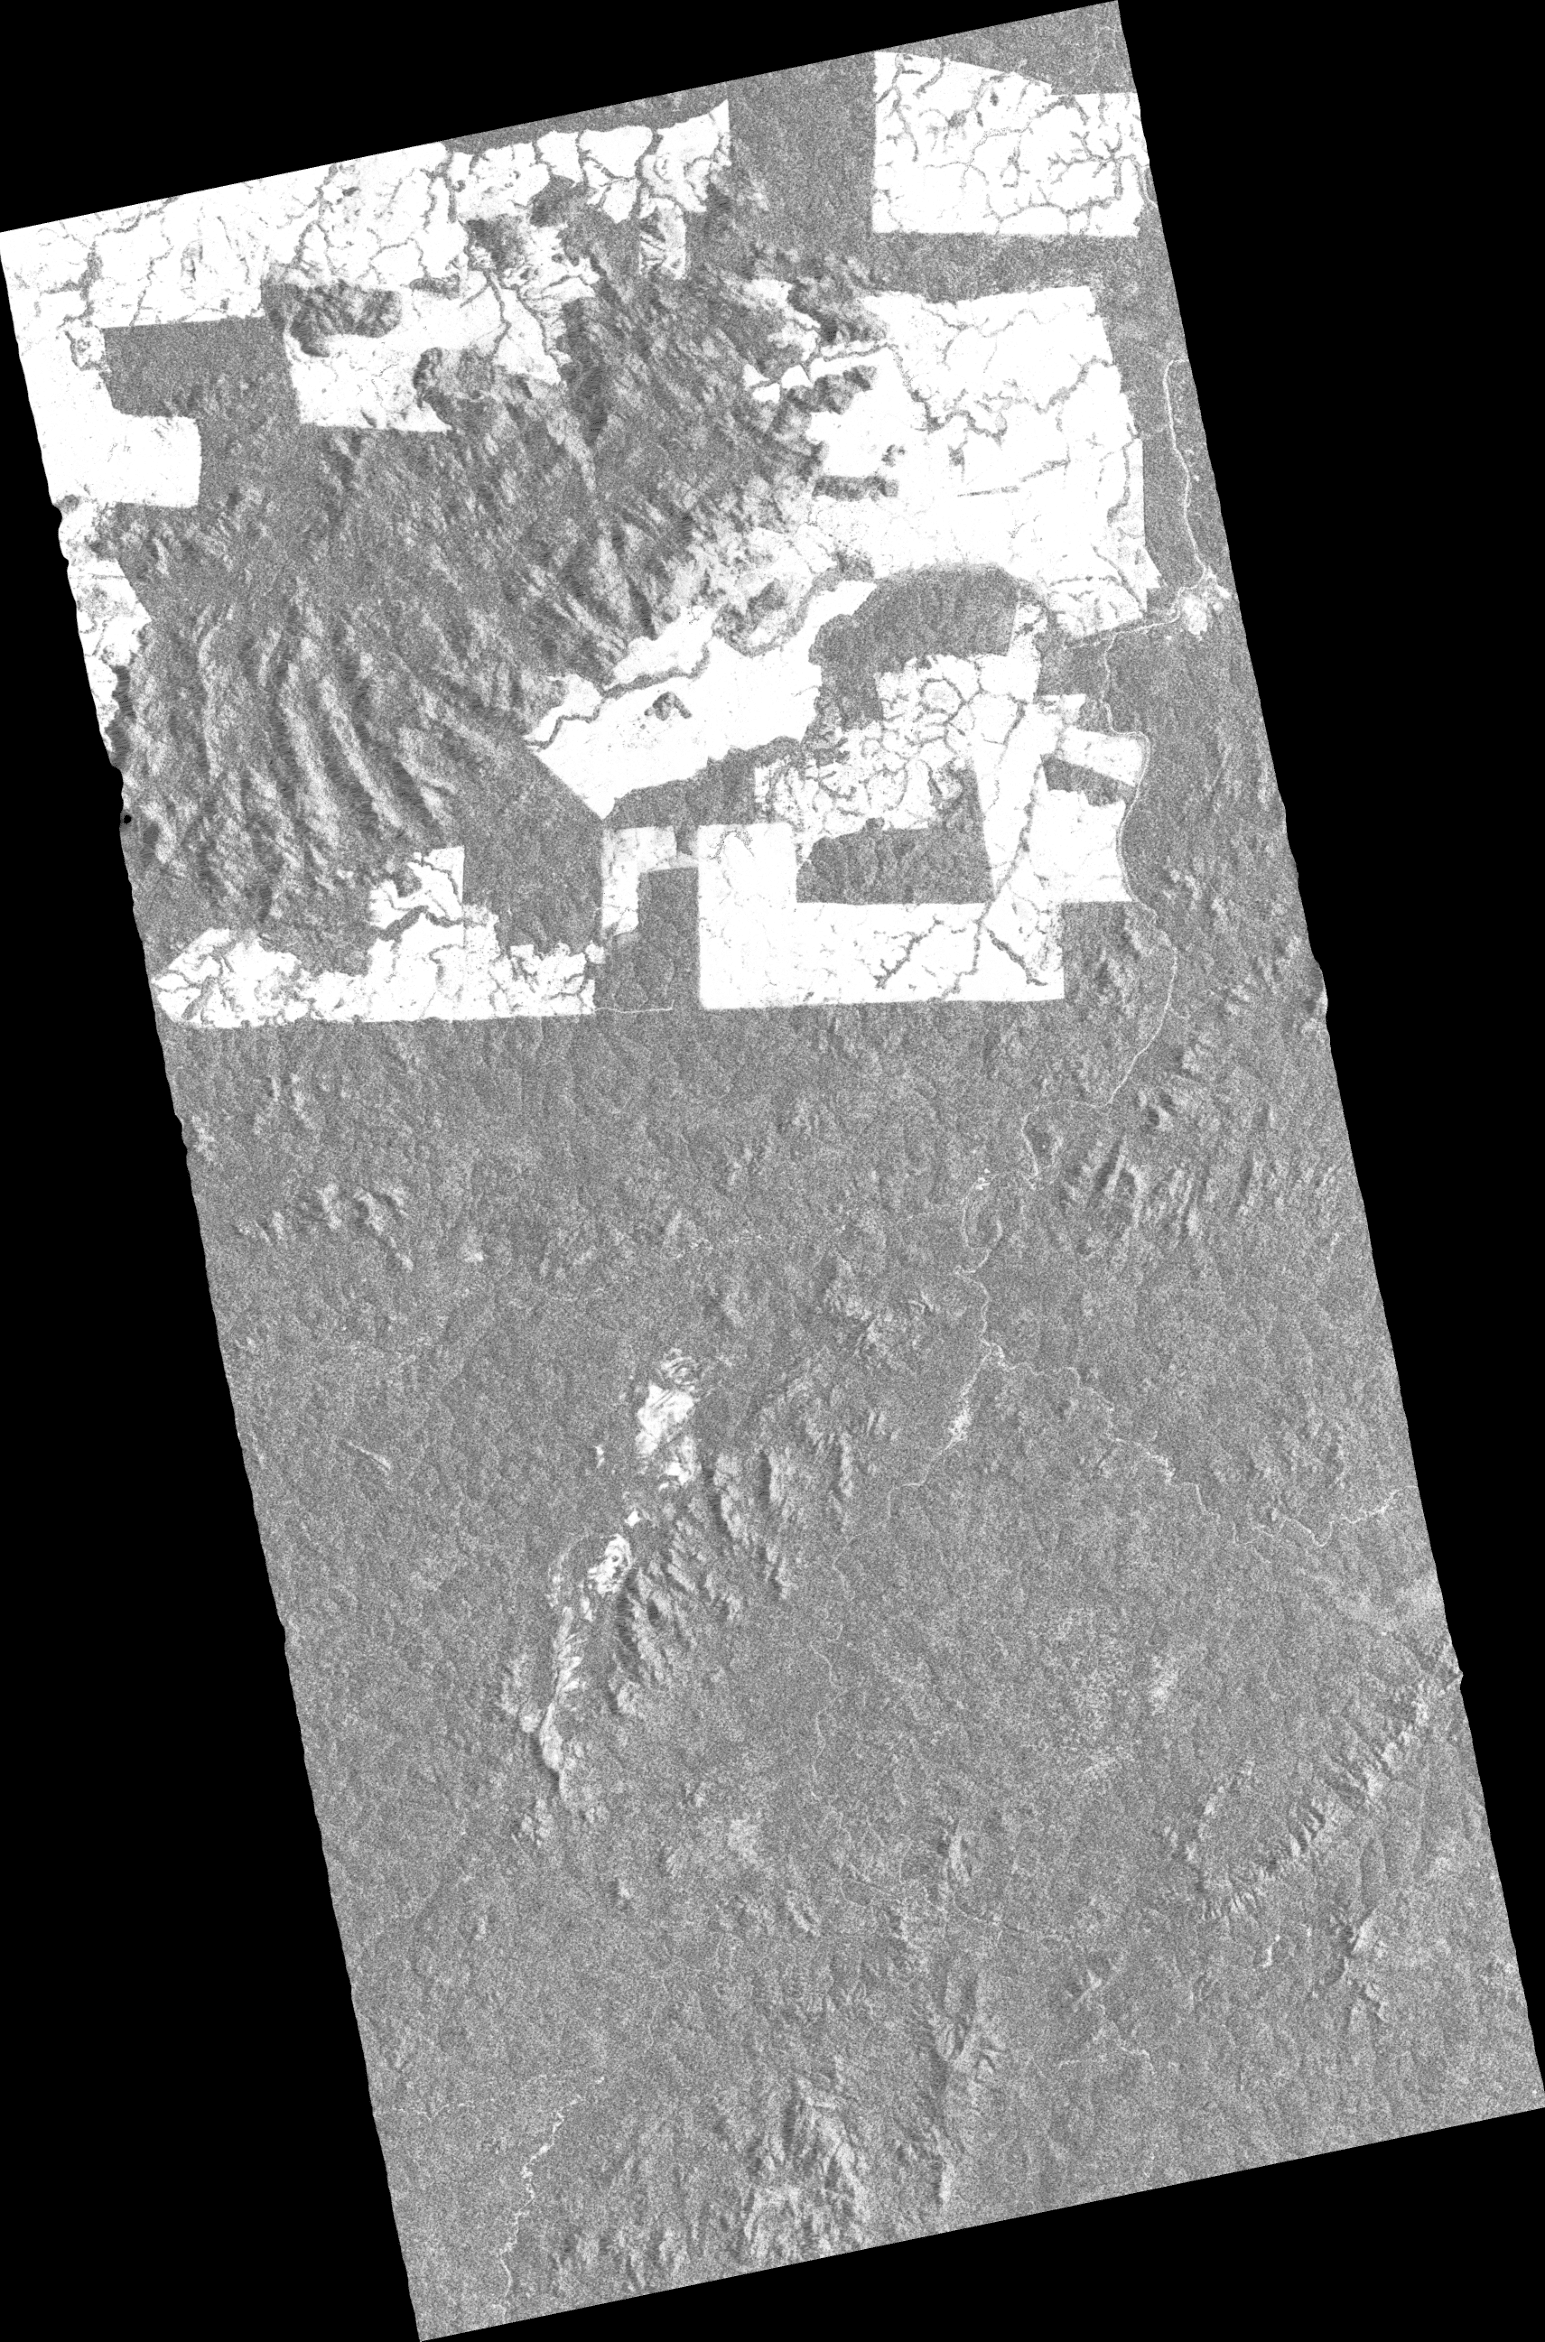
\includegraphics[width=0.8\linewidth]{Chapter4/coSSC_master_gamma_vol.png}
      \caption{Coherence Image of Amazon area.}
    \end{subfigure}
  \caption{Figura}
  \label{fig:asdf}
\end{figure}

Given these two images it will be calculated the result of (\ref{eq:test}) for different displacement vectors
$d=(d_1, d_2)$. It is chosen that the displacement vectors have possibles angle $\theta$ equals to 0$^{\circ}$, 45$^{\circ}$, 90$^{\circ}$ and 135$^{\circ}$, and magnitudes of 1, 2, 3, 4, 5, 6 pixels.
The following tables show the result of the test for the images for areas of forest and deforested areas.



\begin{table}[H]
    \begin{tabular}{ |p{2.5cm}||p{2.5cm}|p{2.5cm}|p{2.5cm}|p{2.5cm}| }
     \hline
     \multicolumn{5}{|c|}{Average Coherence} \\
     \hline
     Distance& $\theta=0$ & $\theta=45$ & $\theta=90$ & $\theta=135$\\
     \hline
        1 &13.46 &7.95 &13.56 &7.96\\
        2 &5.13 &4.06 &5.21 &4.13\\
        3 &4.04 &4.40 &4.13 &4.38\\
        4 &4.19 &5.30 &4.80 &5.18\\
        5 &5.42 &6.71 &5.50 &6.50\\
        6 &6.22 &7.22 &6.39 &6.99\\
     \hline
    
    \end{tabular}
     \caption{$\chi^2$ result for coherence image}
    \label{table:1}
\end{table}

\begin{table}[H]
    \begin{tabular}{ |p{2.5cm}||p{2.5cm}|p{2.5cm}|p{2.5cm}|p{2.5cm}| }
     \hline
     \multicolumn{5}{|c|}{Coherence of forest area} \\
     \hline
     Distance& $\theta=0$ & $\theta=45$ & $\theta=90$ & $\theta=135$\\
     \hline
        1 &13.01 &7.36 &12.68 &7.10\\
        2 &4.52 &3.75 &4.48 &3.77\\
        3 &3.65 &4.32 &3.91 &4.34\\
        4 &4.14 &5.20 &4.58 &5.10\\
        5 &5.12 &6.57 &5.21 &6.41\\
        6 &6.91 &7.06 &6.08 &6.87\\
     \hline
    \end{tabular}
     \caption{$\chi^2$ result for coherence in forest areas}
    \label{table:2}
\end{table}

\begin{table}[H]
    \begin{tabular}{ |p{2.5cm}||p{2.5cm}|p{2.5cm}|p{2.5cm}|p{2.5cm}| }
     \hline
     \multicolumn{5}{|c|}{Coherence of deforested area} \\
     \hline
     Distance& $\theta=0$ & $\theta=45$ & $\theta=90$ & $\theta=135$\\
     \hline
        1 &10.58 &7.28 &10.84 &7.16\\
        2 &4.94 &3.33 &5.37 &3.24\\
        3 &3.26 &2.71 &3.78 &2.63\\
        4 &3.11 &3.20 &3.64 &3.11\\
        5 &3.73 &4.04 &4.09 &3.95\\
        6 &4.29 &4.33 &4.51 &4.29\\
     \hline
    \end{tabular}
     \caption{$\chi^2$ result for coherence in deforested areas}
    \label{table:3}
\end{table}

\begin{table}[H]
    \begin{tabular}{ |p{2.5cm}||p{2.5cm}|p{2.5cm}|p{2.5cm}|p{2.5cm}| }
     \hline
     \multicolumn{5}{|c|}{$\beta^0$ of forest area} \\
     \hline
     Distance& $\theta=0$ & $\theta=45$ & $\theta=90$ & $\theta=135$\\
     \hline
        1 &1.26 &0.63 &1.59 &0.73\\
        2 &0.28 &0.20 &0.42 &0.24\\
        3 &0.22 &0.24 &0.26 &0.23\\
        4 &0.29 &0.29 &0.28 &0.27\\
        5 &0.35 &0.39 &0.31 &0.35\\
        6 &0.39 &0.44 &0.37 &0.39\\
     \hline
    \end{tabular}
     \caption{$\chi^2$ result for $\beta^0$ in forest areas}
    \label{table:4}
\end{table}

\begin{table}[H]
    \begin{tabular}{ |p{2.5cm}||p{2.5cm}|p{2.5cm}|p{2.5cm}|p{2.5cm}| }
     \hline
     \multicolumn{5}{|c|}{$\beta^0$ of deforested area} \\
     \hline
     Distance& $\theta=0$ & $\theta=45$ & $\theta=90$ & $\theta=135$\\
     \hline
        1 &0.82 &0.43 &1.07 &0.50\\
        2 &0.22 &0.14 &0.33 &0.15\\
        3 &0.15 &0.14 &0.20 &0.13\\
        4 &0.17 &0.17 &0.19 &0.16\\
        5 &0.20 &0.22 &0.02 &0.21\\
        6 &0.23 &0.26 &0.23 &0.25\\
     \hline
    \end{tabular}
     \caption{$\chi^2$ result for $\beta^0$ in deforested areas}
    \label{table:5}
\end{table}

Analyzing the tables above we can see that choosing pixels that are closer in the image gives the maximum information for texture calculations (this means that there are no hidden patterns/structures in the images analyzed). According to the tables, until the rest of this work the displacement vector used will always be equals to $d=(0, 1)$.


\subsection{The GLCM textures results}
Let us visualize the texture results for the Coherence image above.
It was computed 7 different textures for the coherence image above: the ASM, contrast, correlation, dissimilarity, energy, entropy and homogeneity.
These textures can be visualized below
\newpage
\begin{figure}[H]
  \centering
  \begin{subfigure}[b]{0.4\linewidth}
    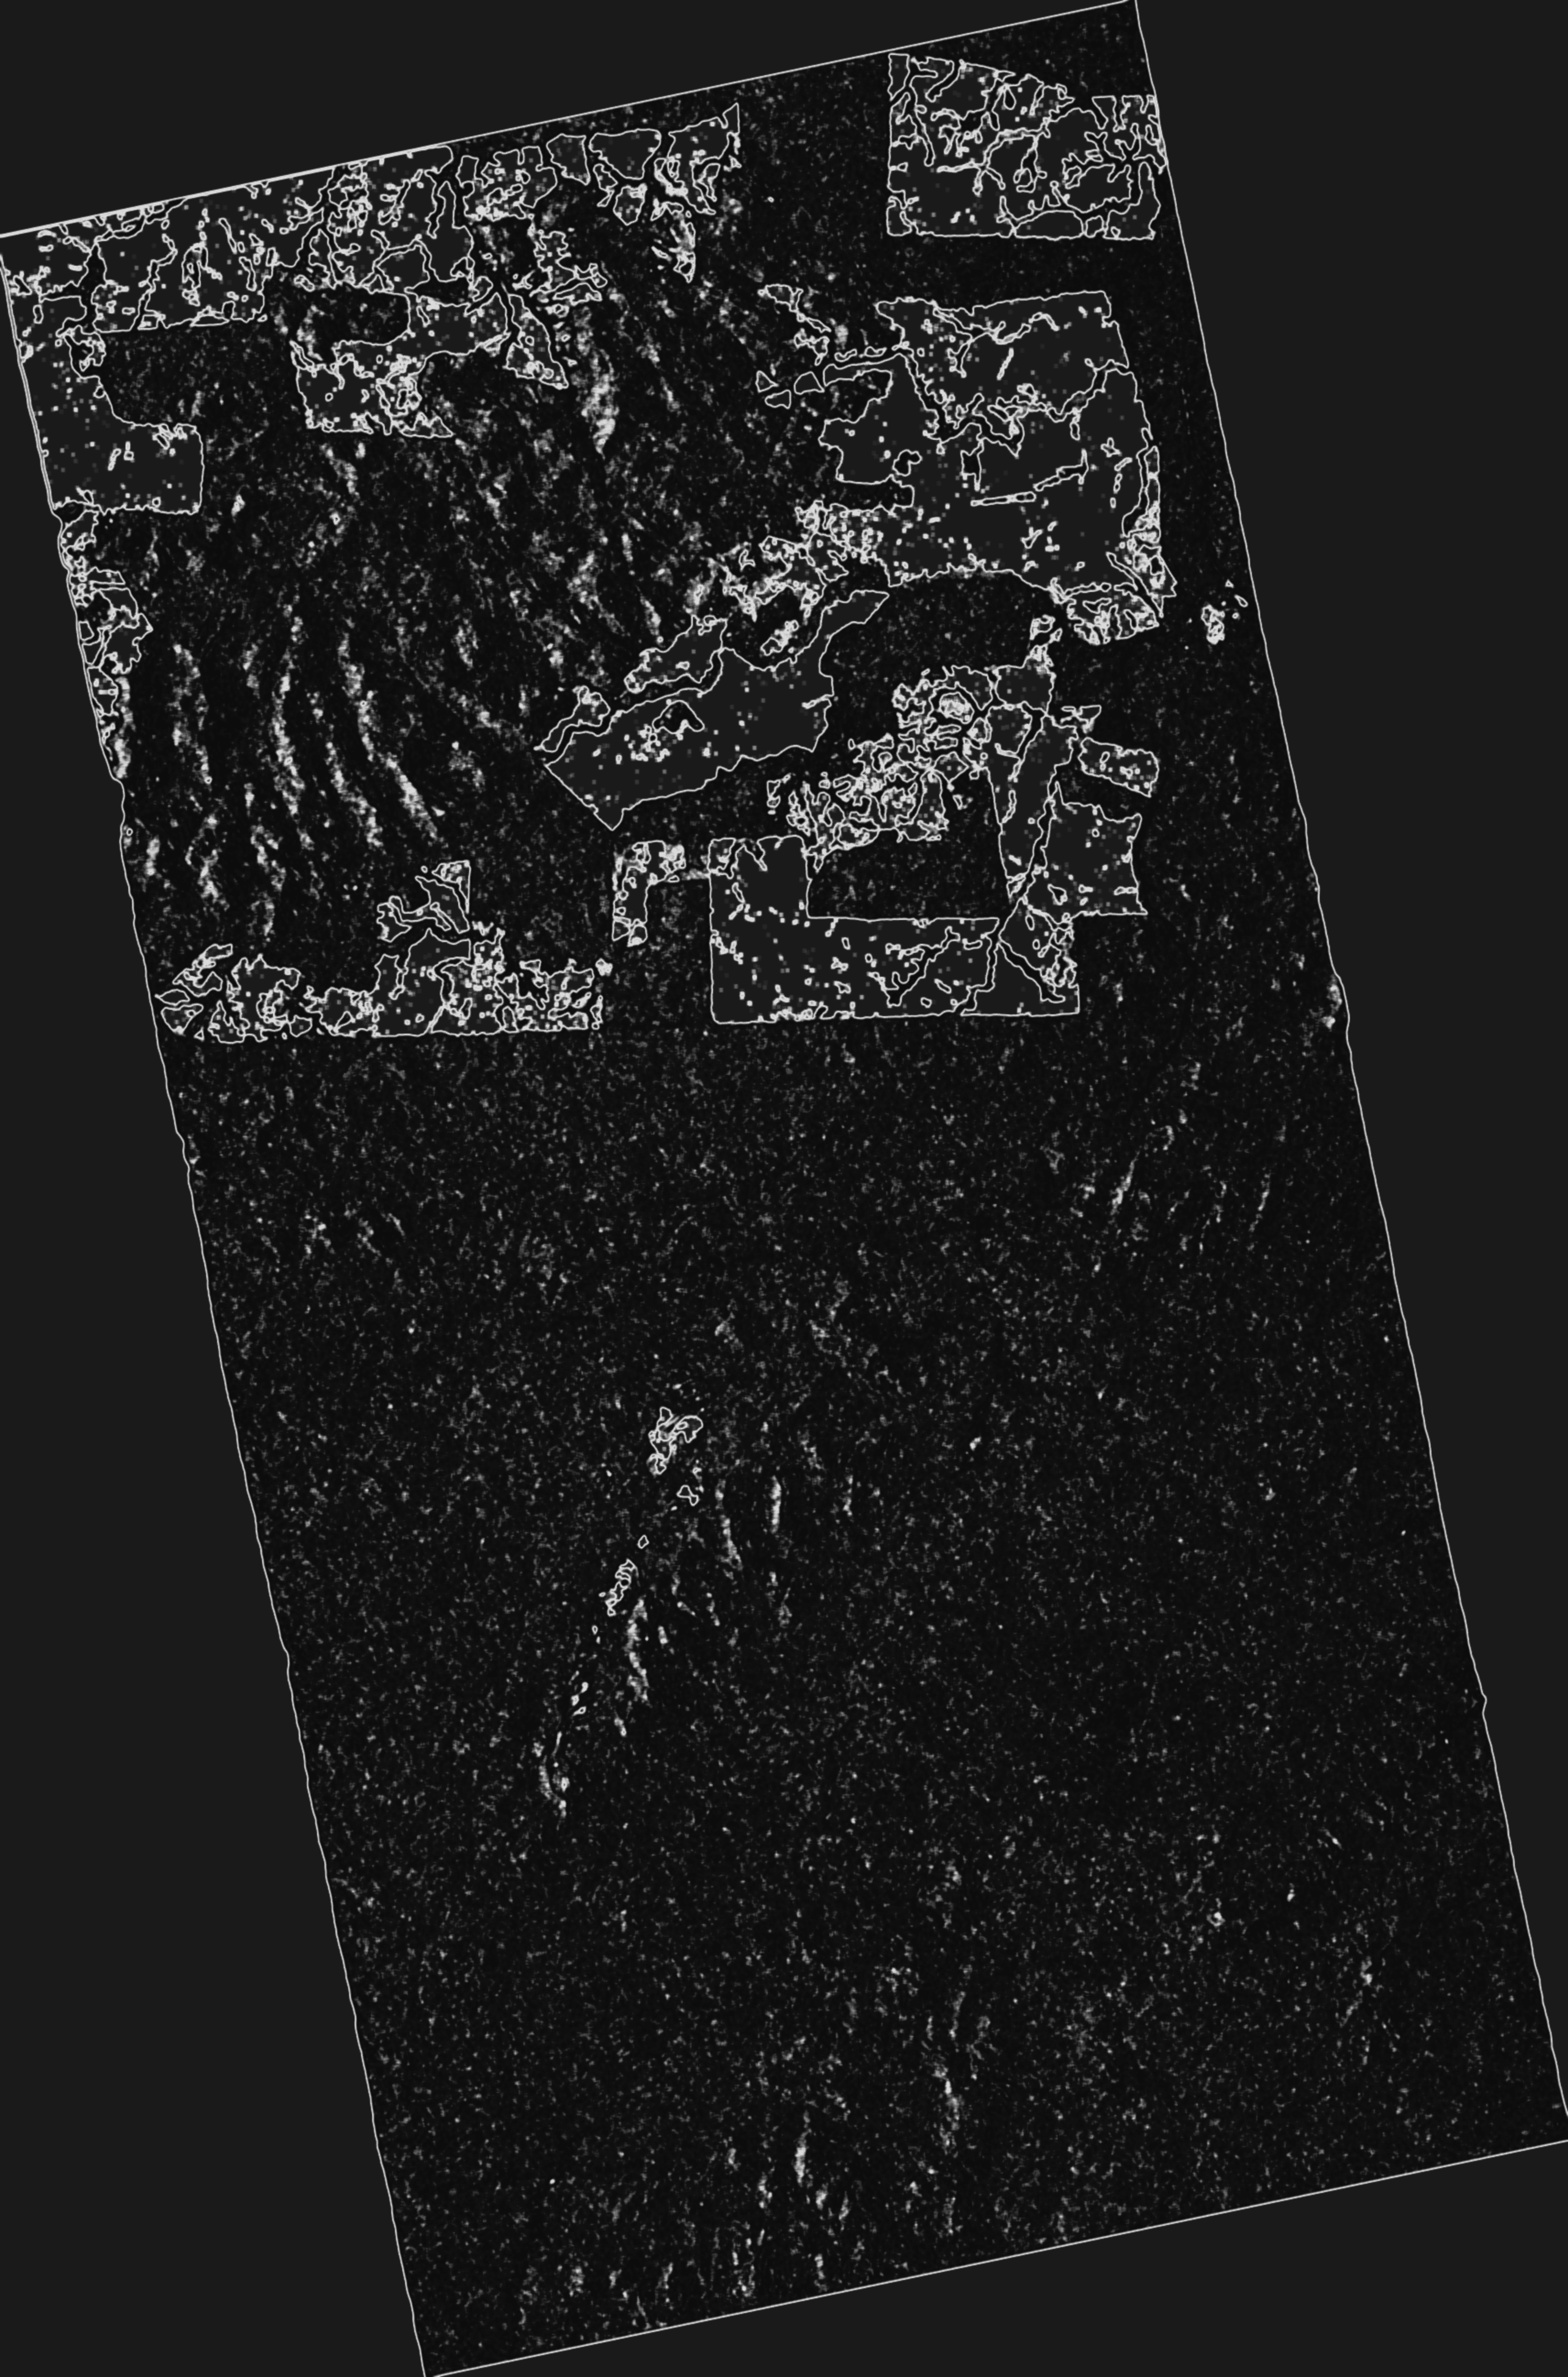
\includegraphics[width=\linewidth]{Chapter4/glcm_textures/ASMimage.png}
     \caption{ASM texture of Coherence Image}
  \end{subfigure}
  \begin{subfigure}[b]{0.4\linewidth}
    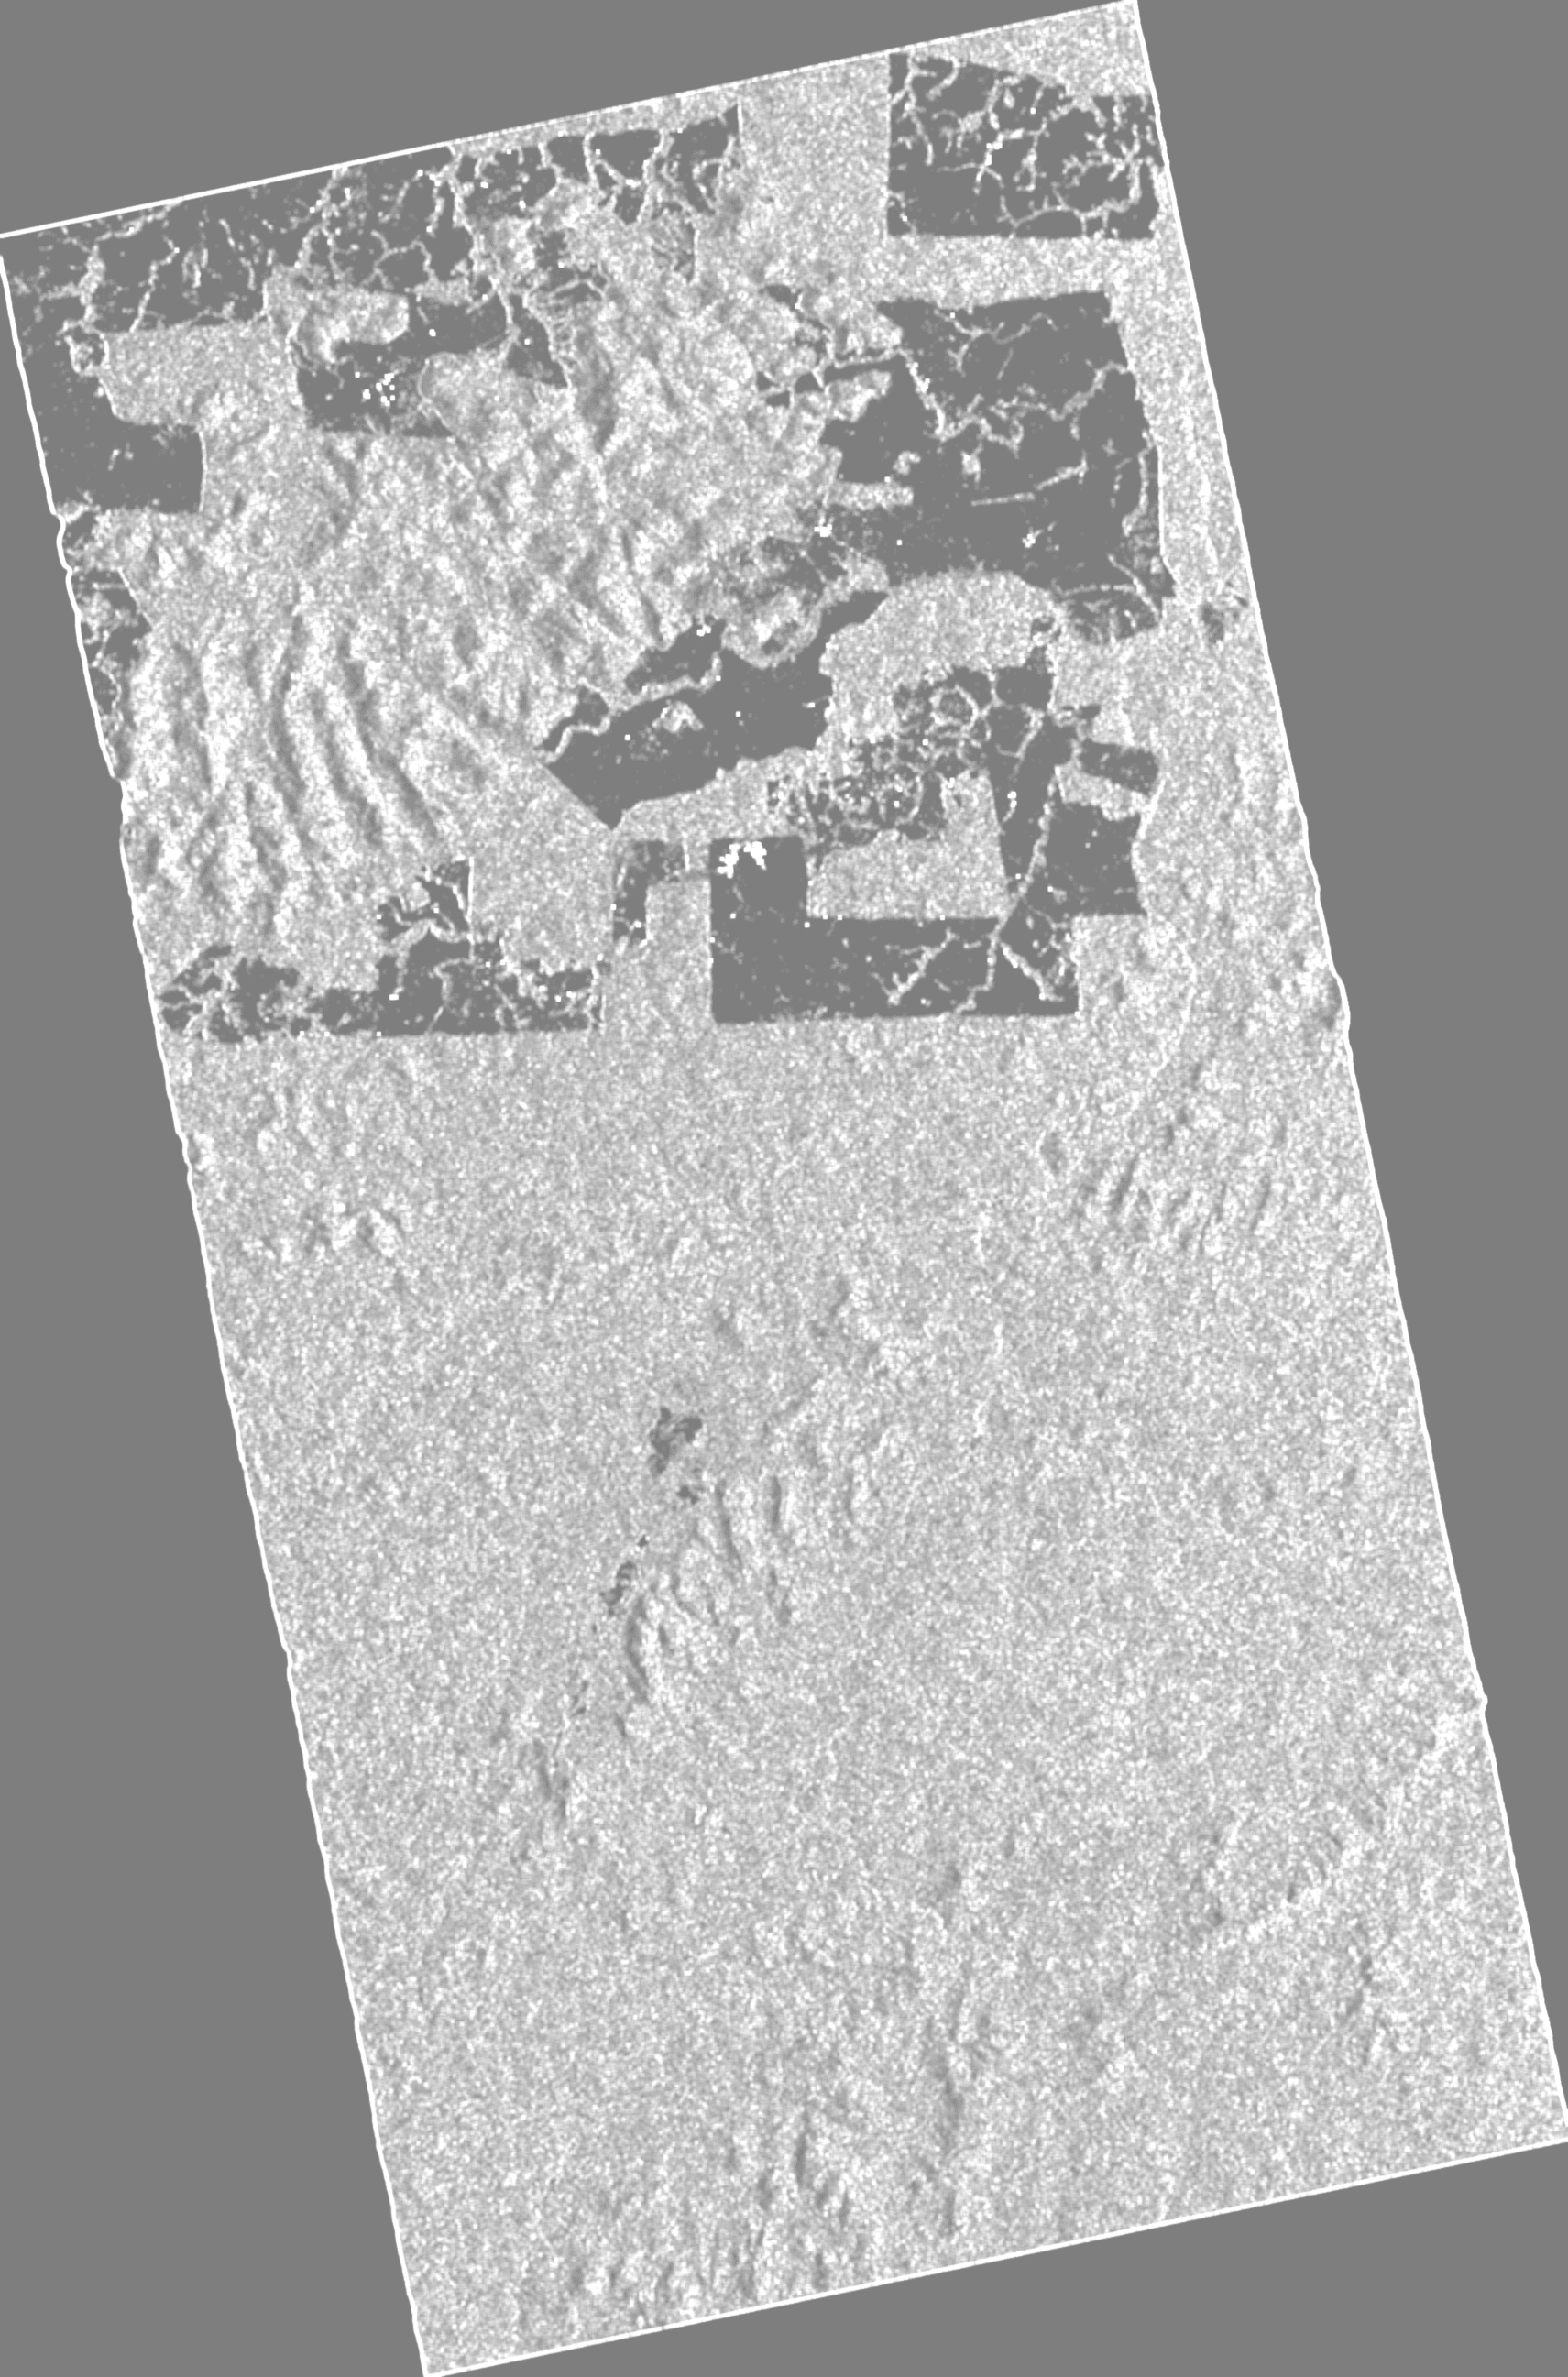
\includegraphics[width=\linewidth]{Chapter4/glcm_textures/contrastimage.png}
    \caption{Contrast texture of Coherence Image}
  \end{subfigure}
  \begin{subfigure}[b]{0.4\linewidth}
    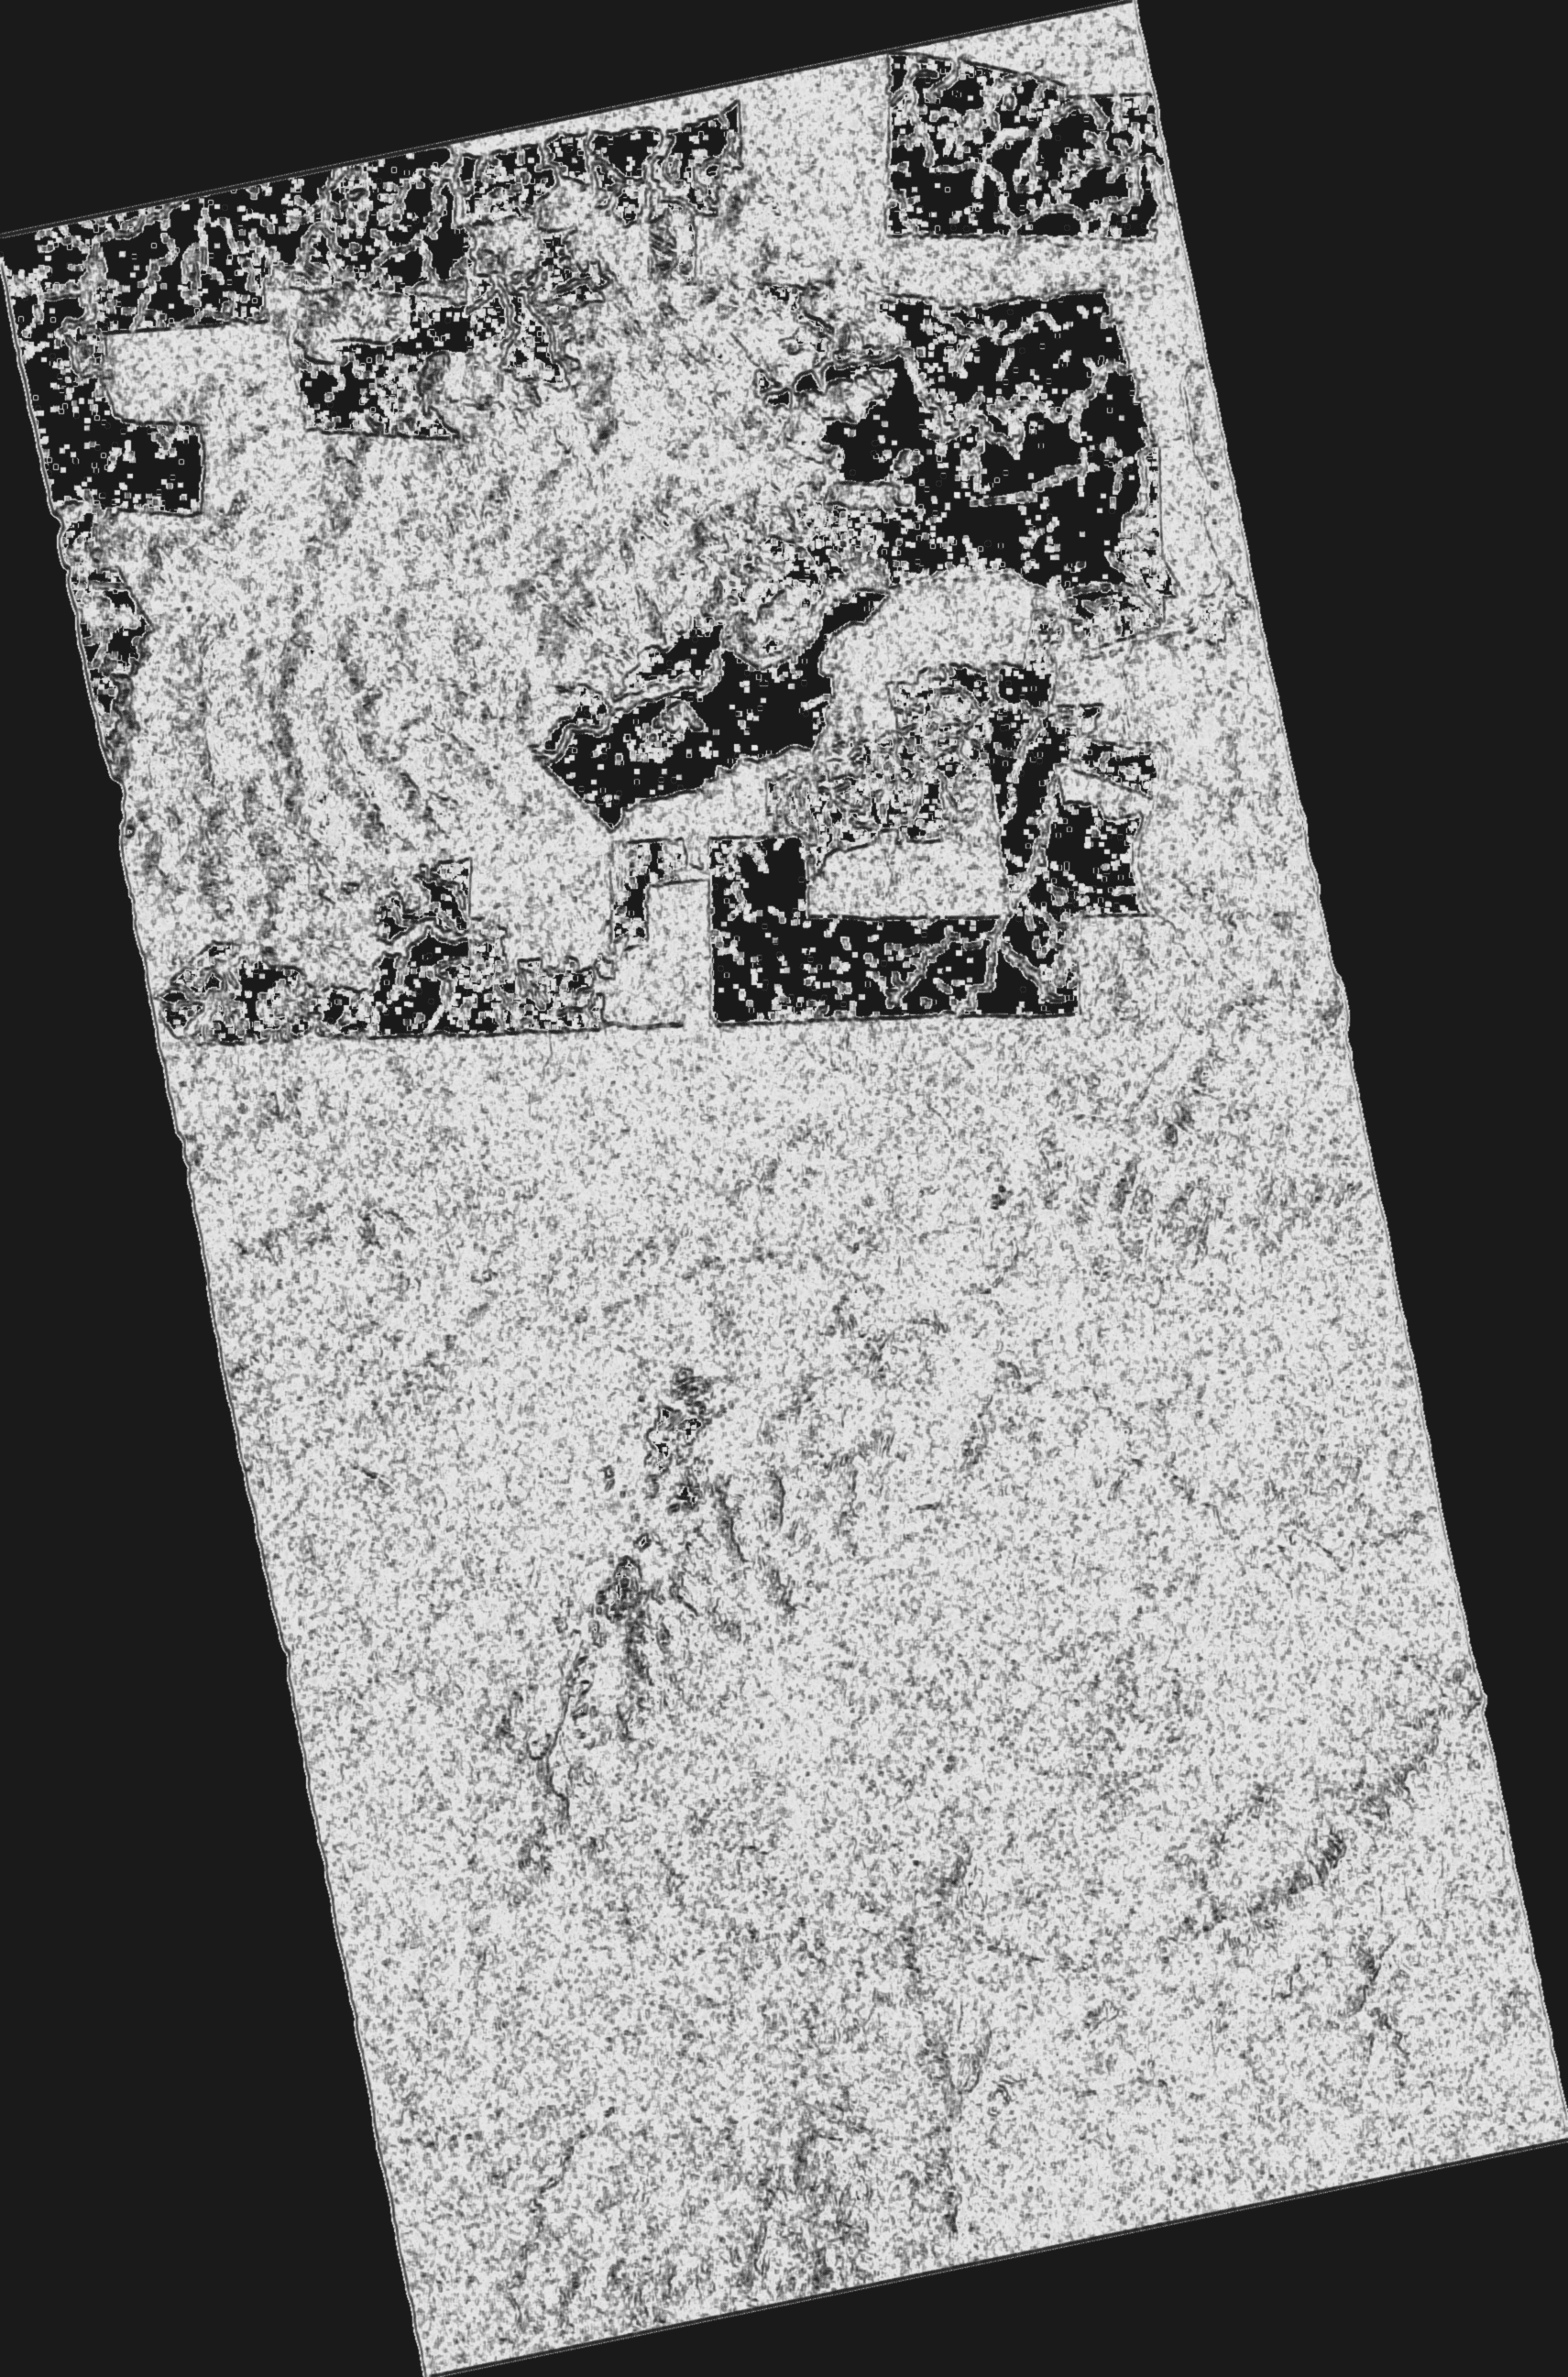
\includegraphics[width=\linewidth]{Chapter4/glcm_textures/correlationimage.png}
    \caption{Correlation texture of Coherence Image}
  \end{subfigure}
  \begin{subfigure}[b]{0.4\linewidth}
    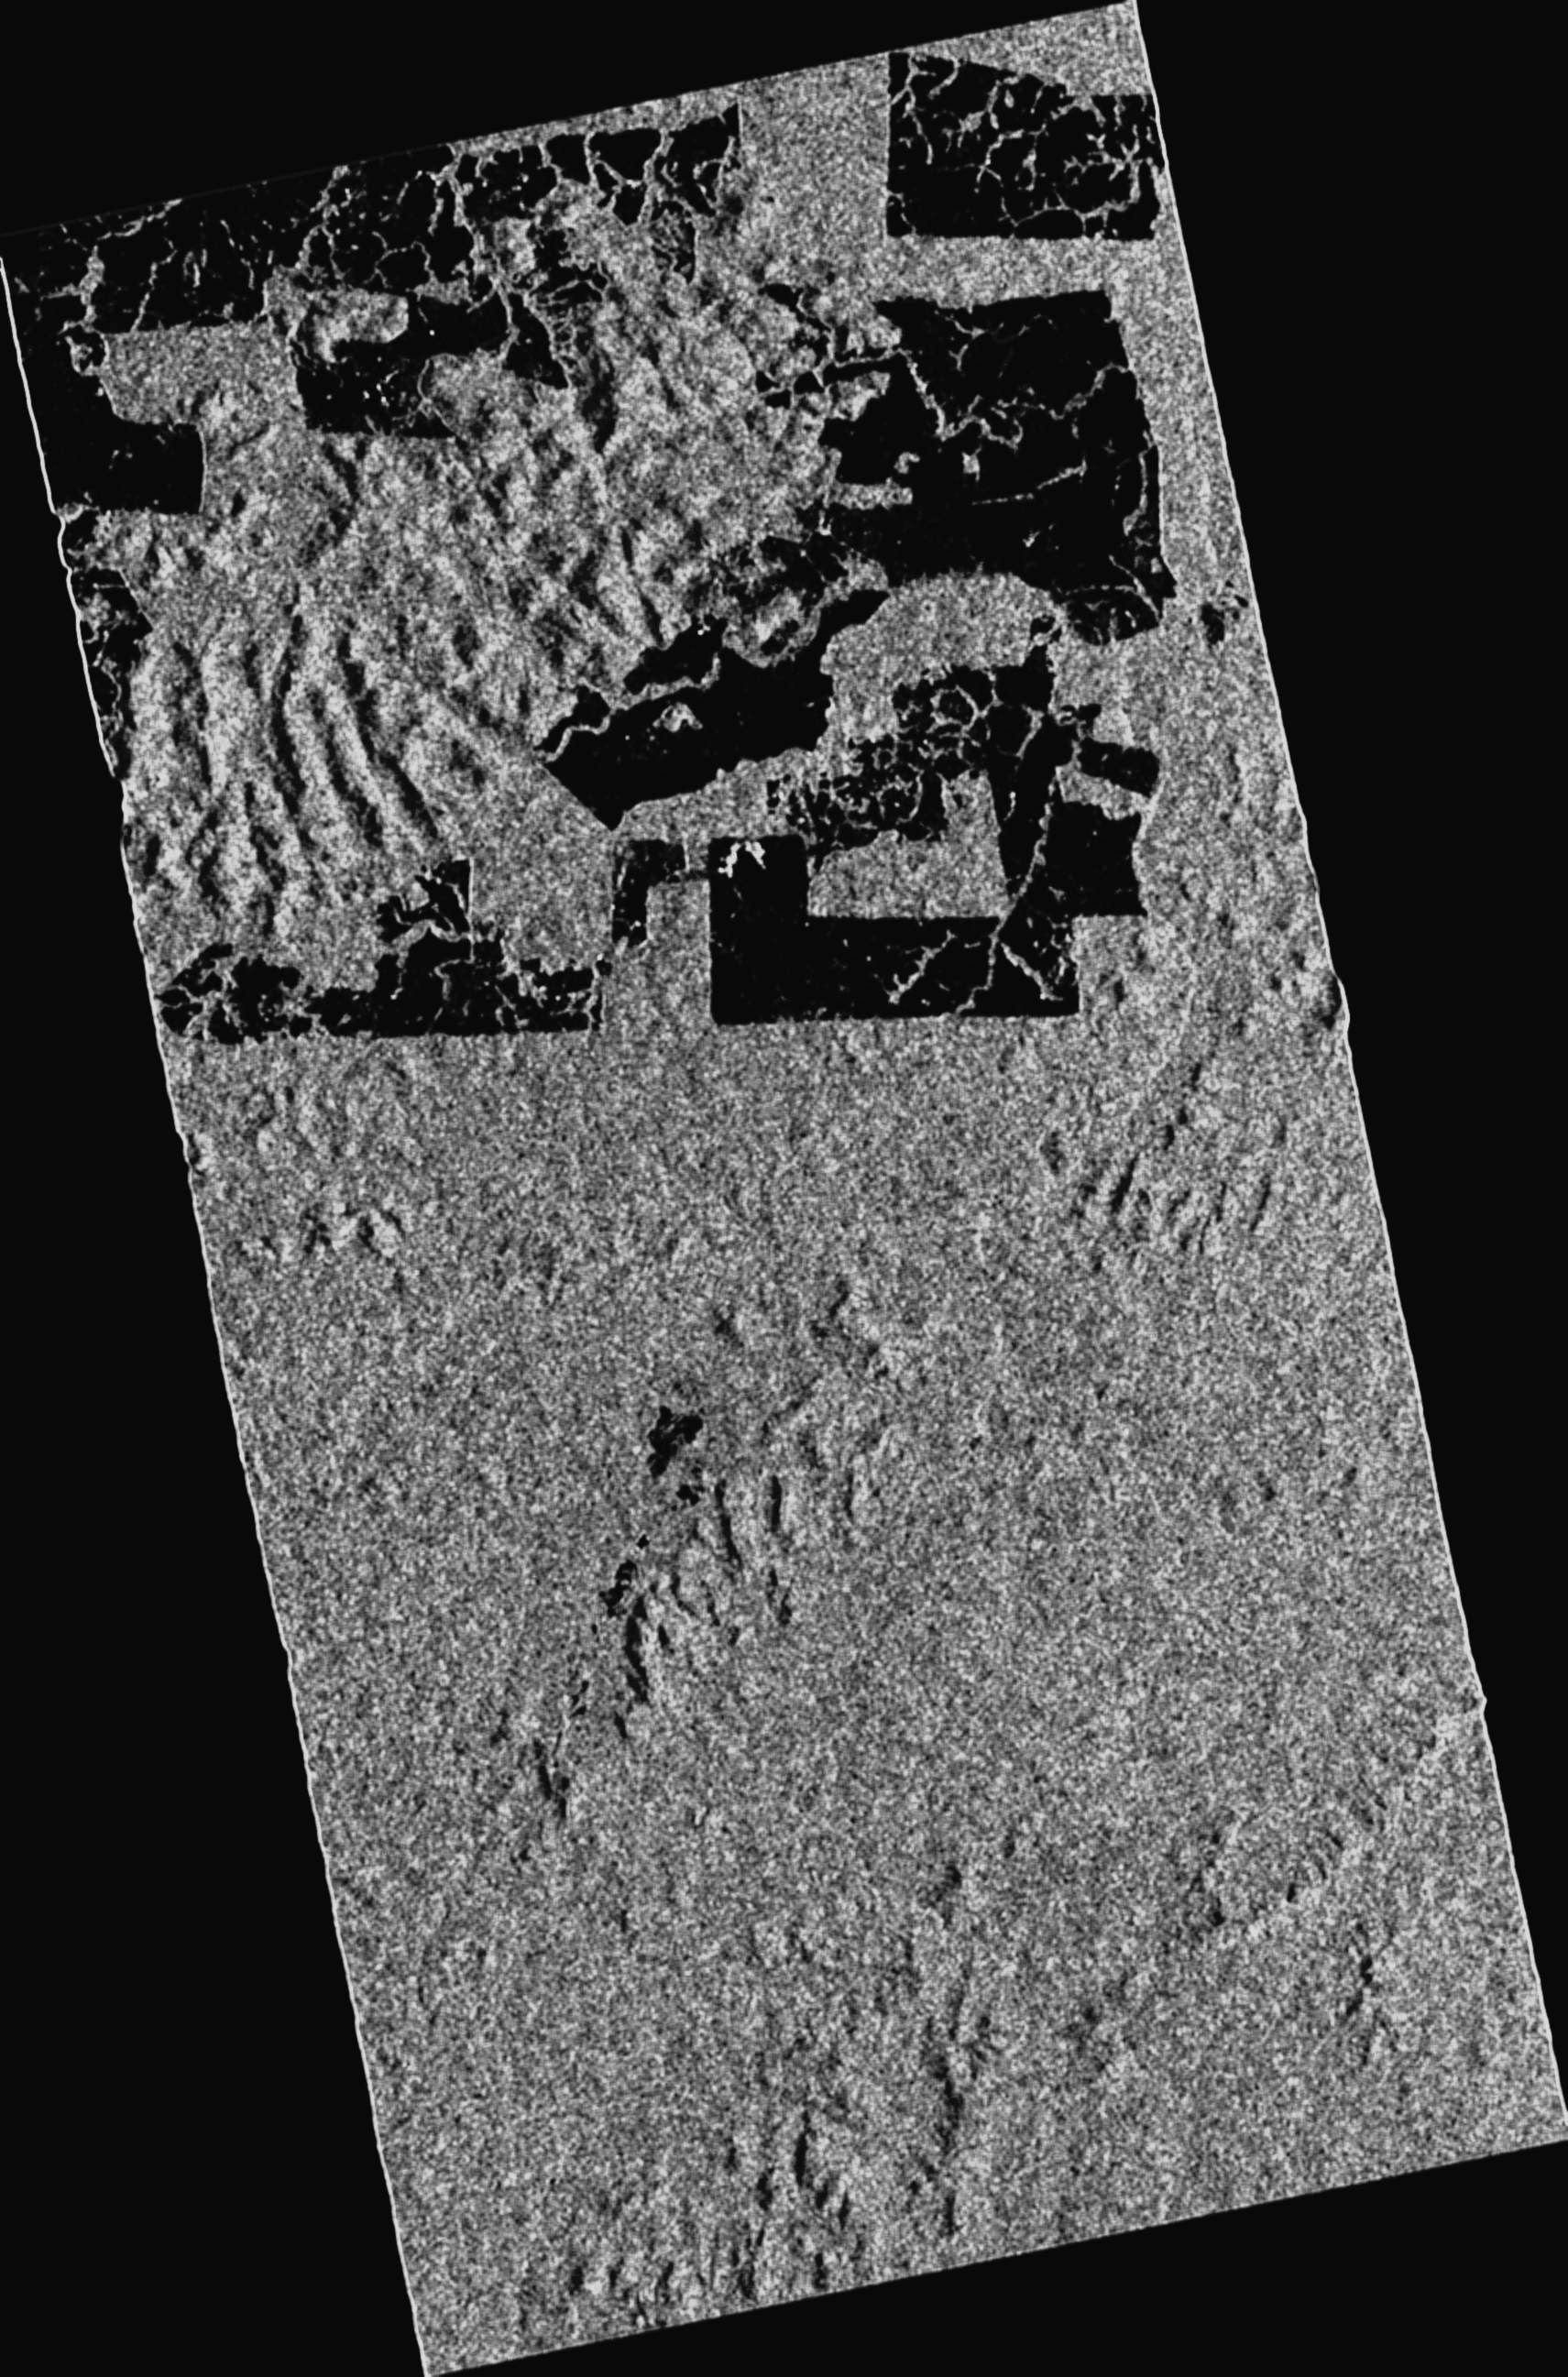
\includegraphics[width=\linewidth]{Chapter4/glcm_textures/dissimilarityimage.png}
    \caption{Dissimilarity texture of Coherence Image}
  \end{subfigure}
\end{figure}
\newpage
\begin{figure}[H]\ContinuedFloat
  \begin{subfigure}[b]{0.4\linewidth}
    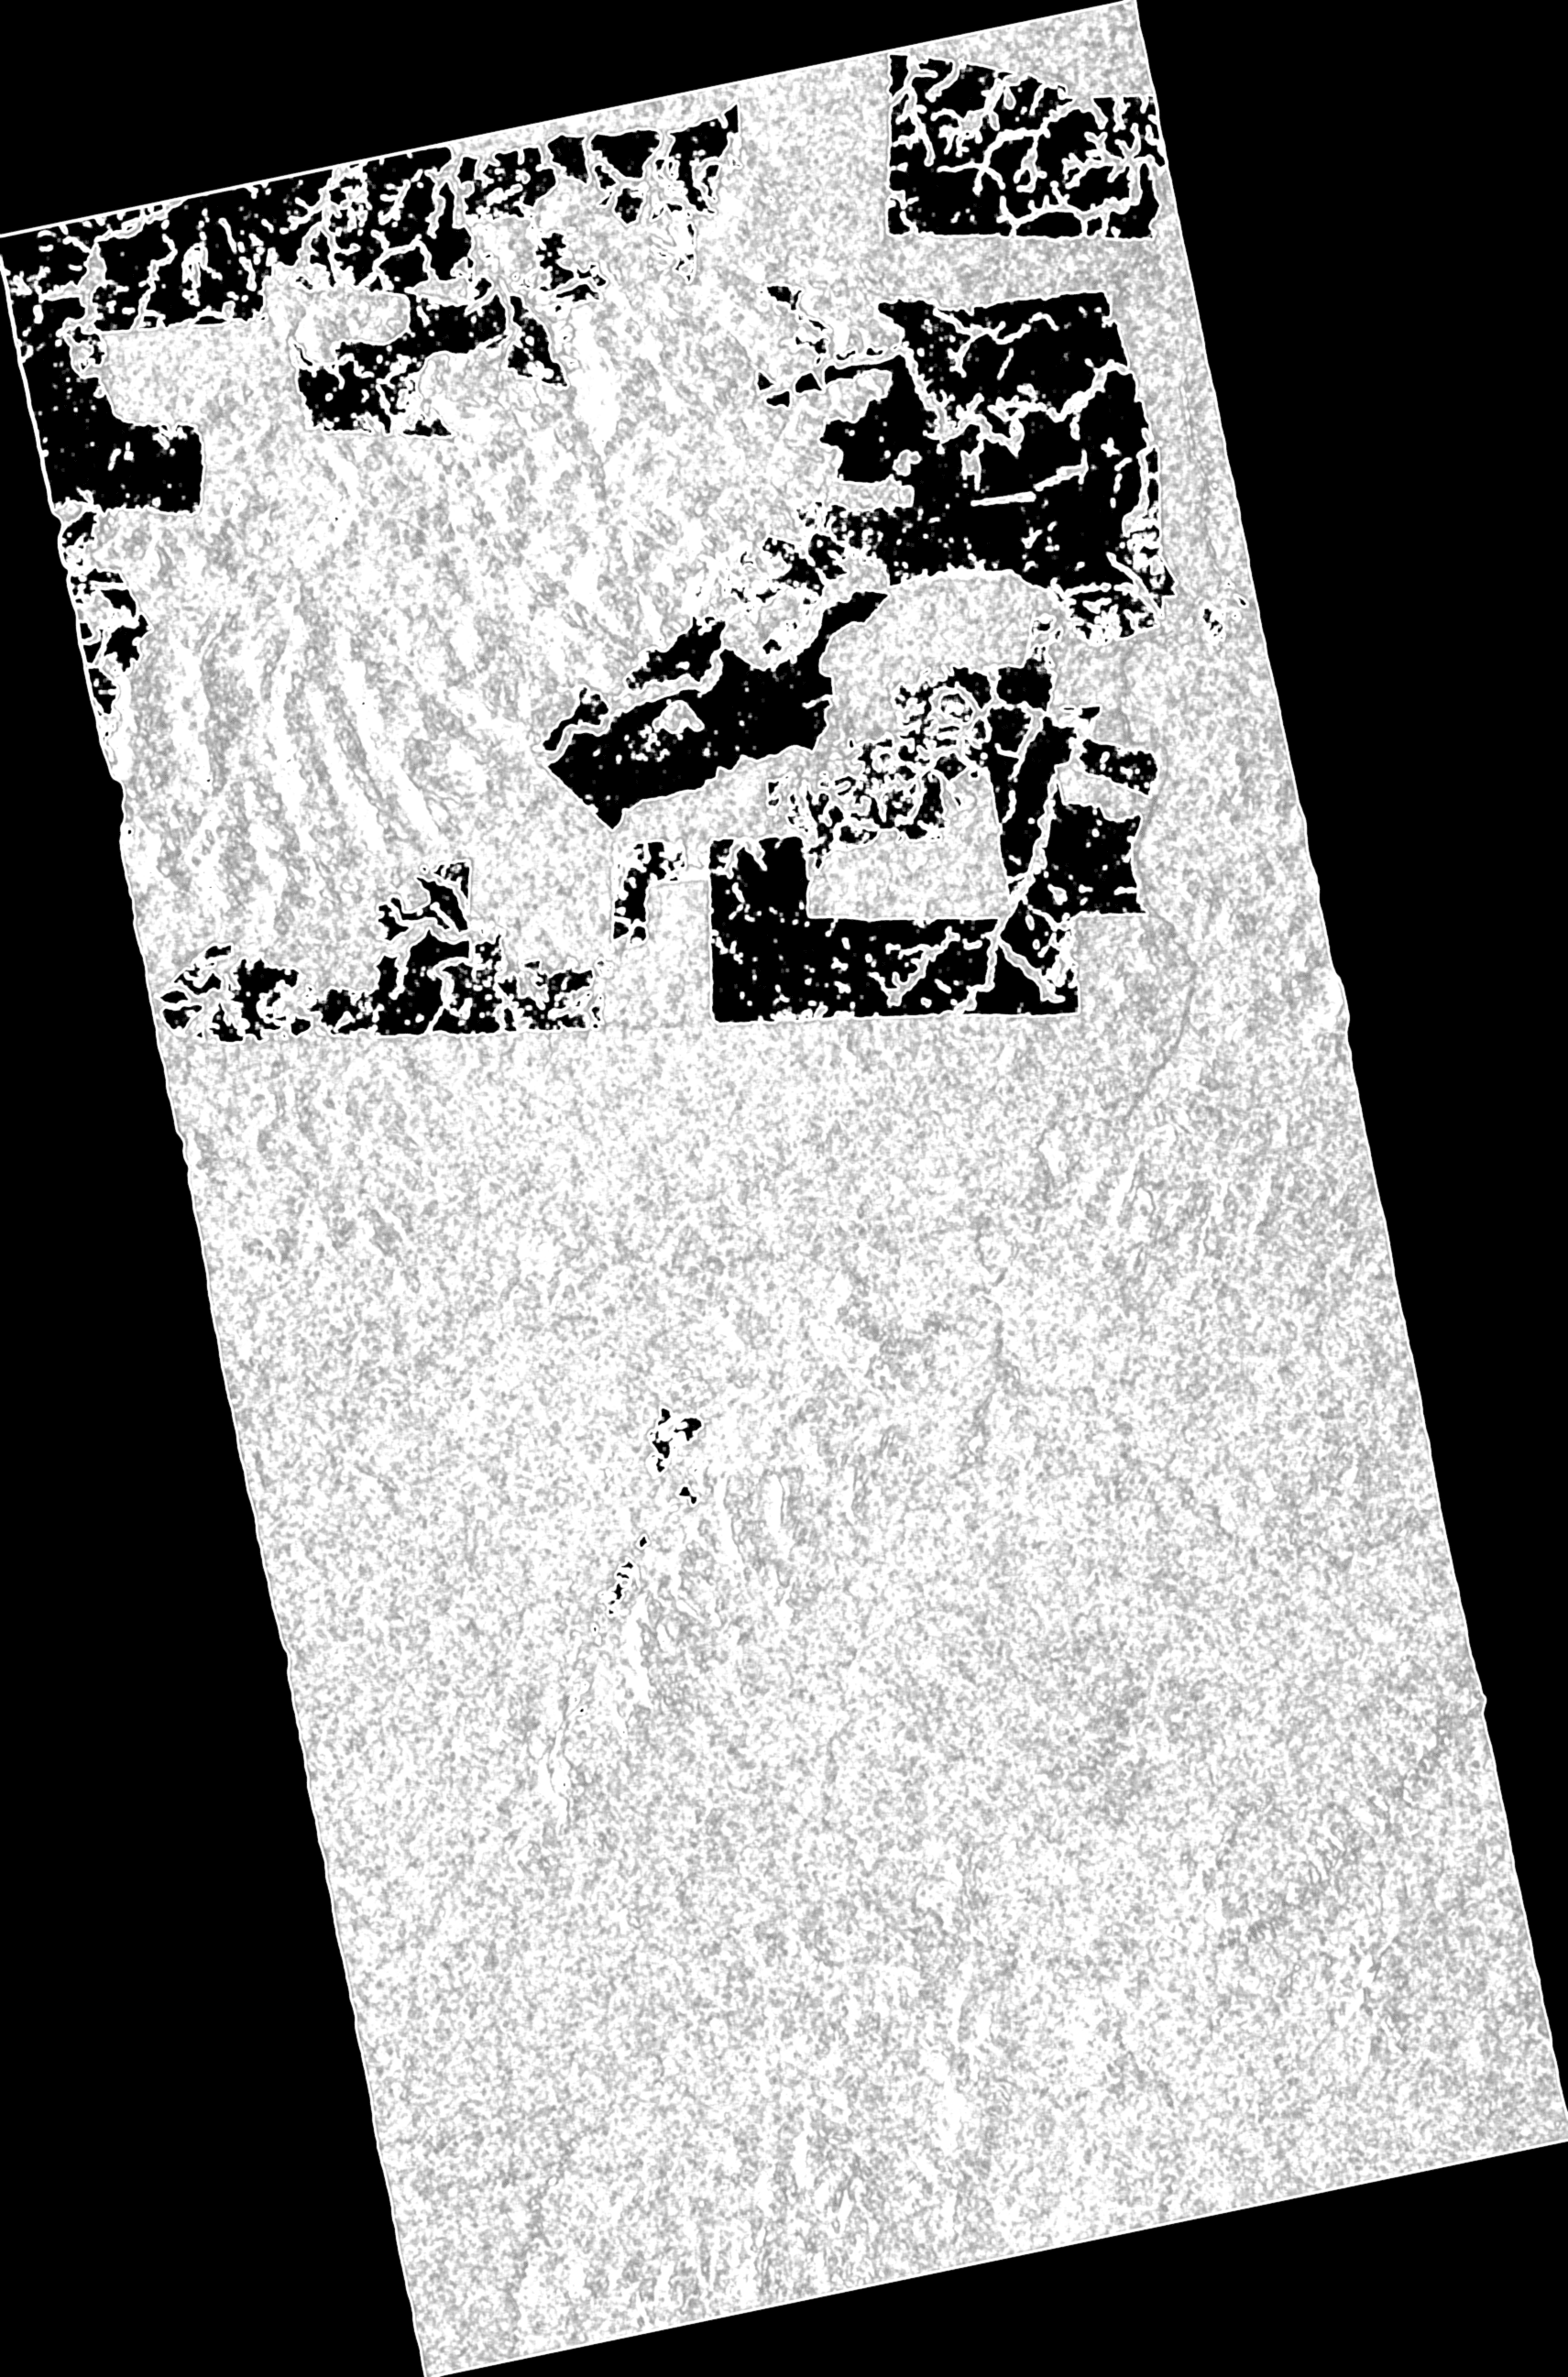
\includegraphics[width=\linewidth]{Chapter4/glcm_textures/energyimage.png}
    \caption{Energy texture of Coherence Image}
  \end{subfigure}
  \begin{subfigure}[b]{0.4\linewidth}
    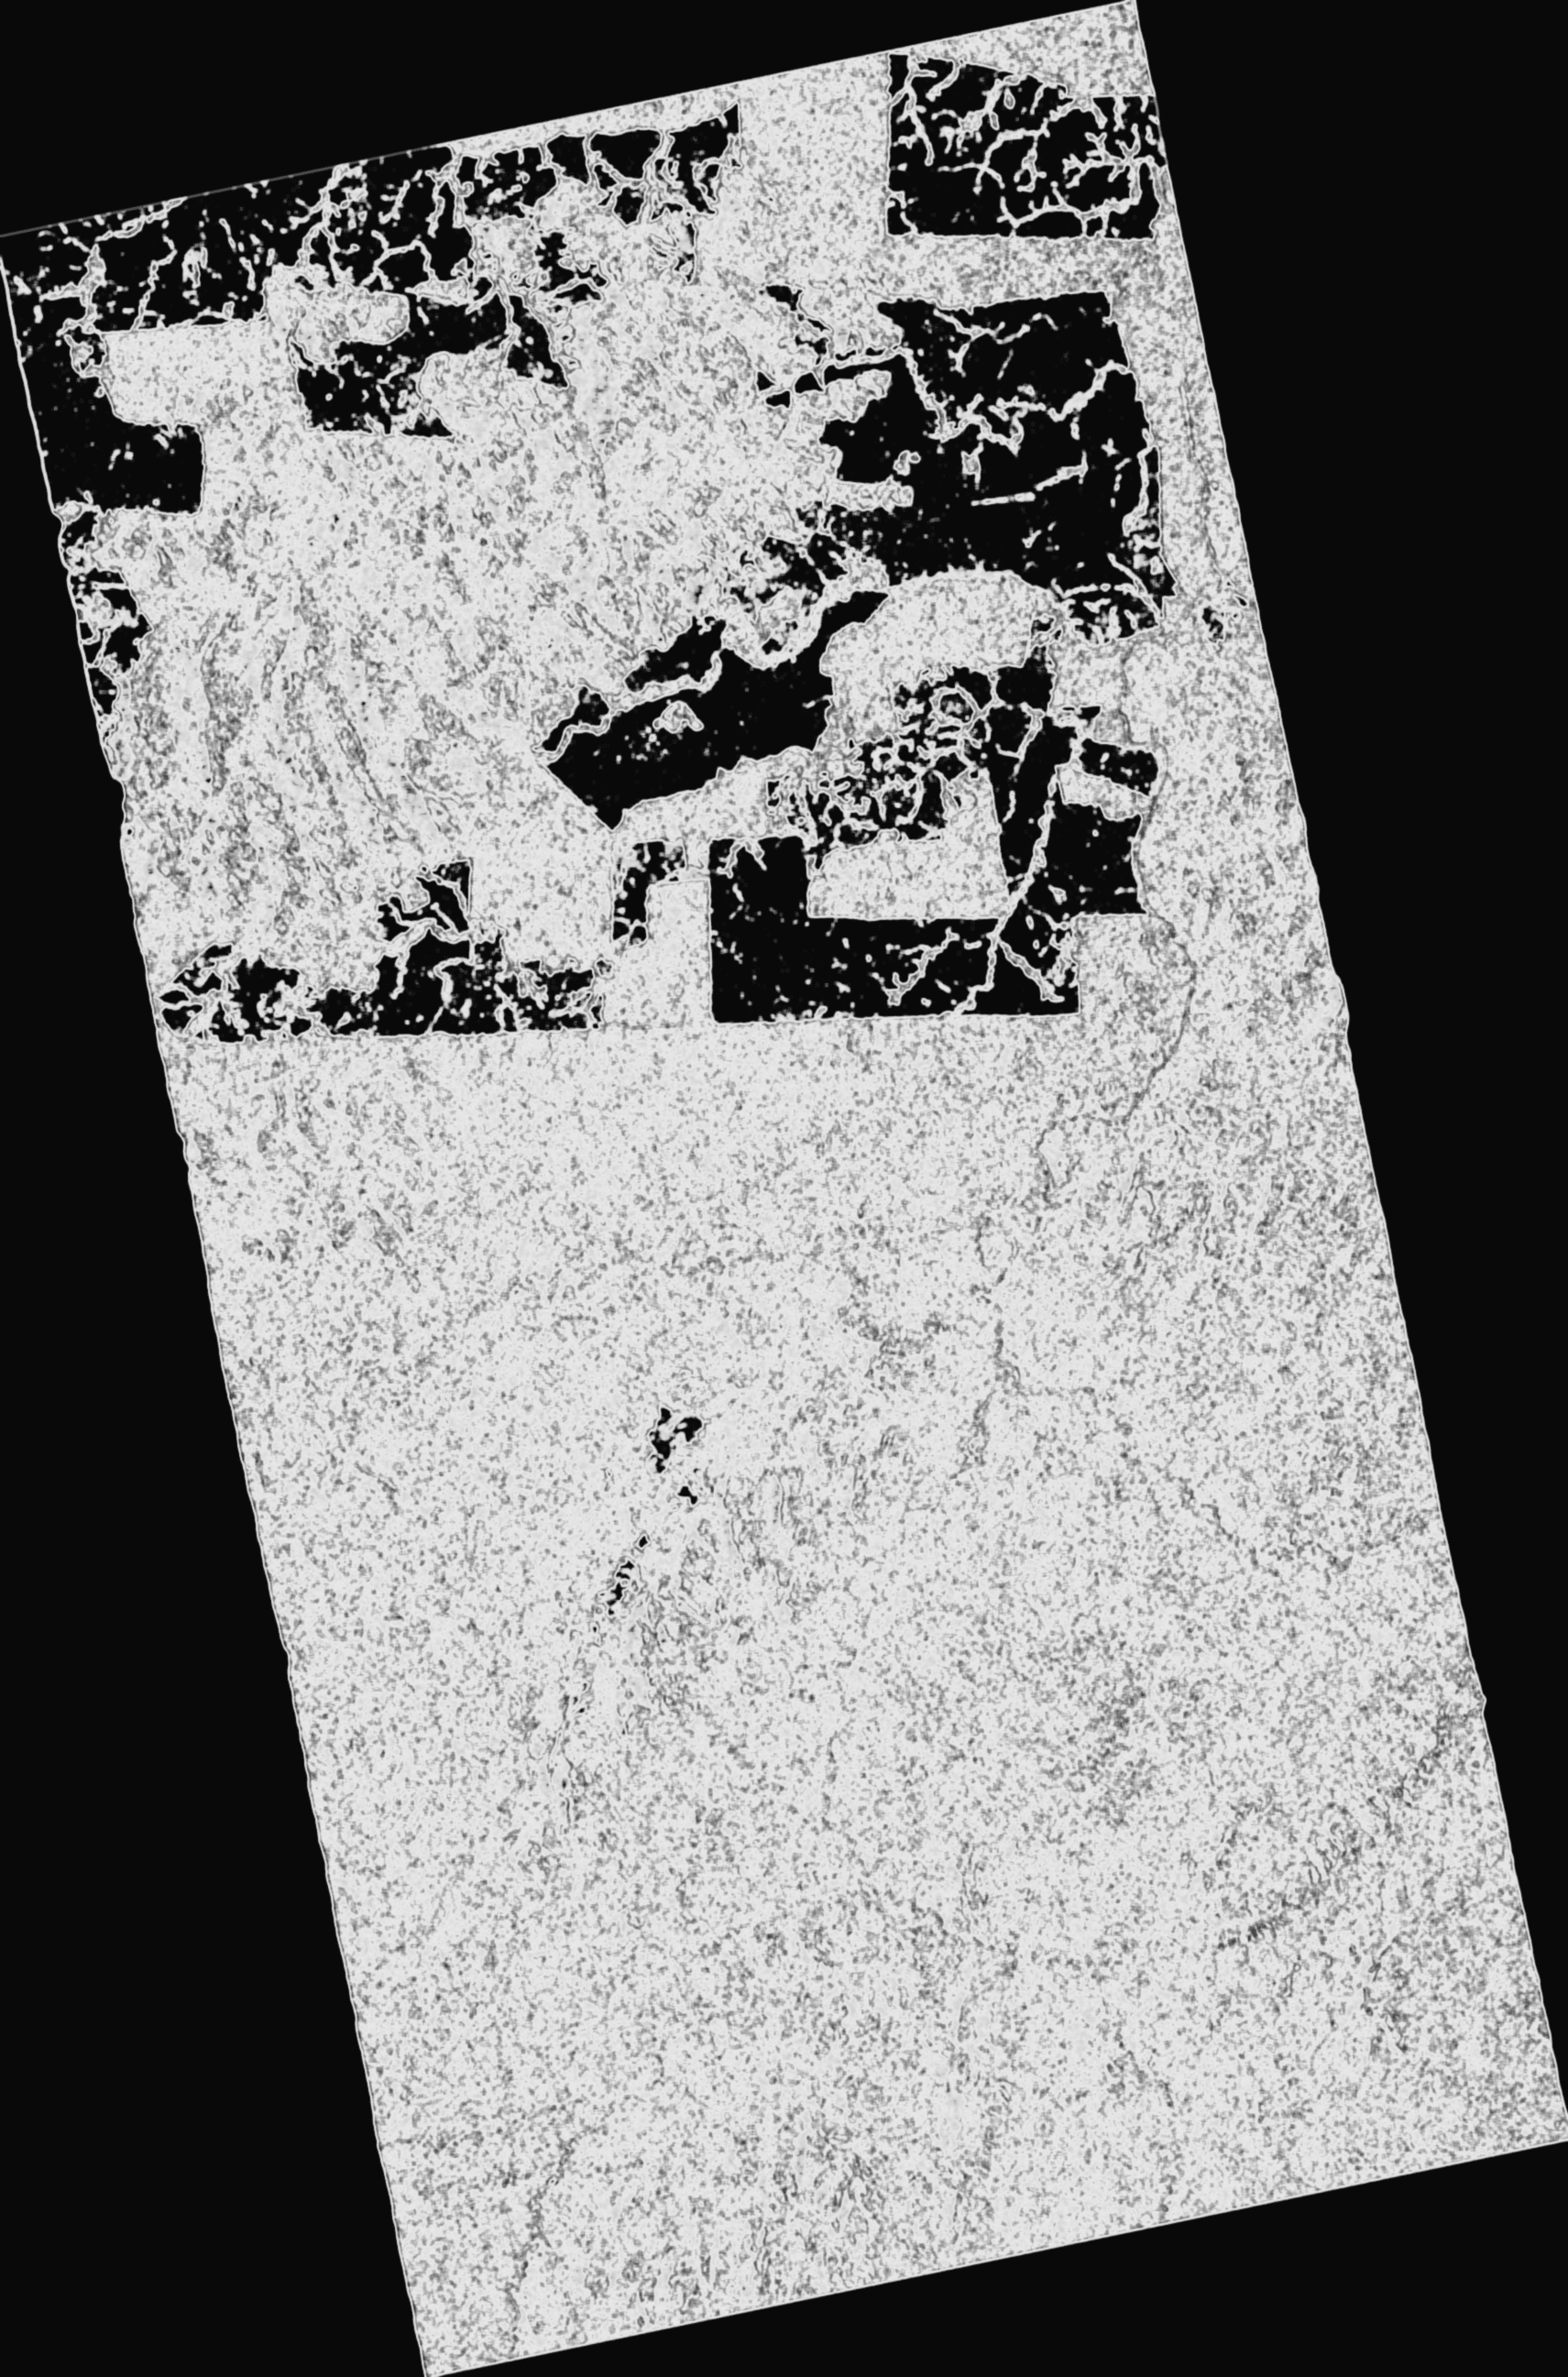
\includegraphics[width=\linewidth]{Chapter4/glcm_textures/entropyimage.png}
    \caption{Entropy texture of Coherence Image}
  \end{subfigure}
  \begin{subfigure}[b]{0.4\linewidth}
    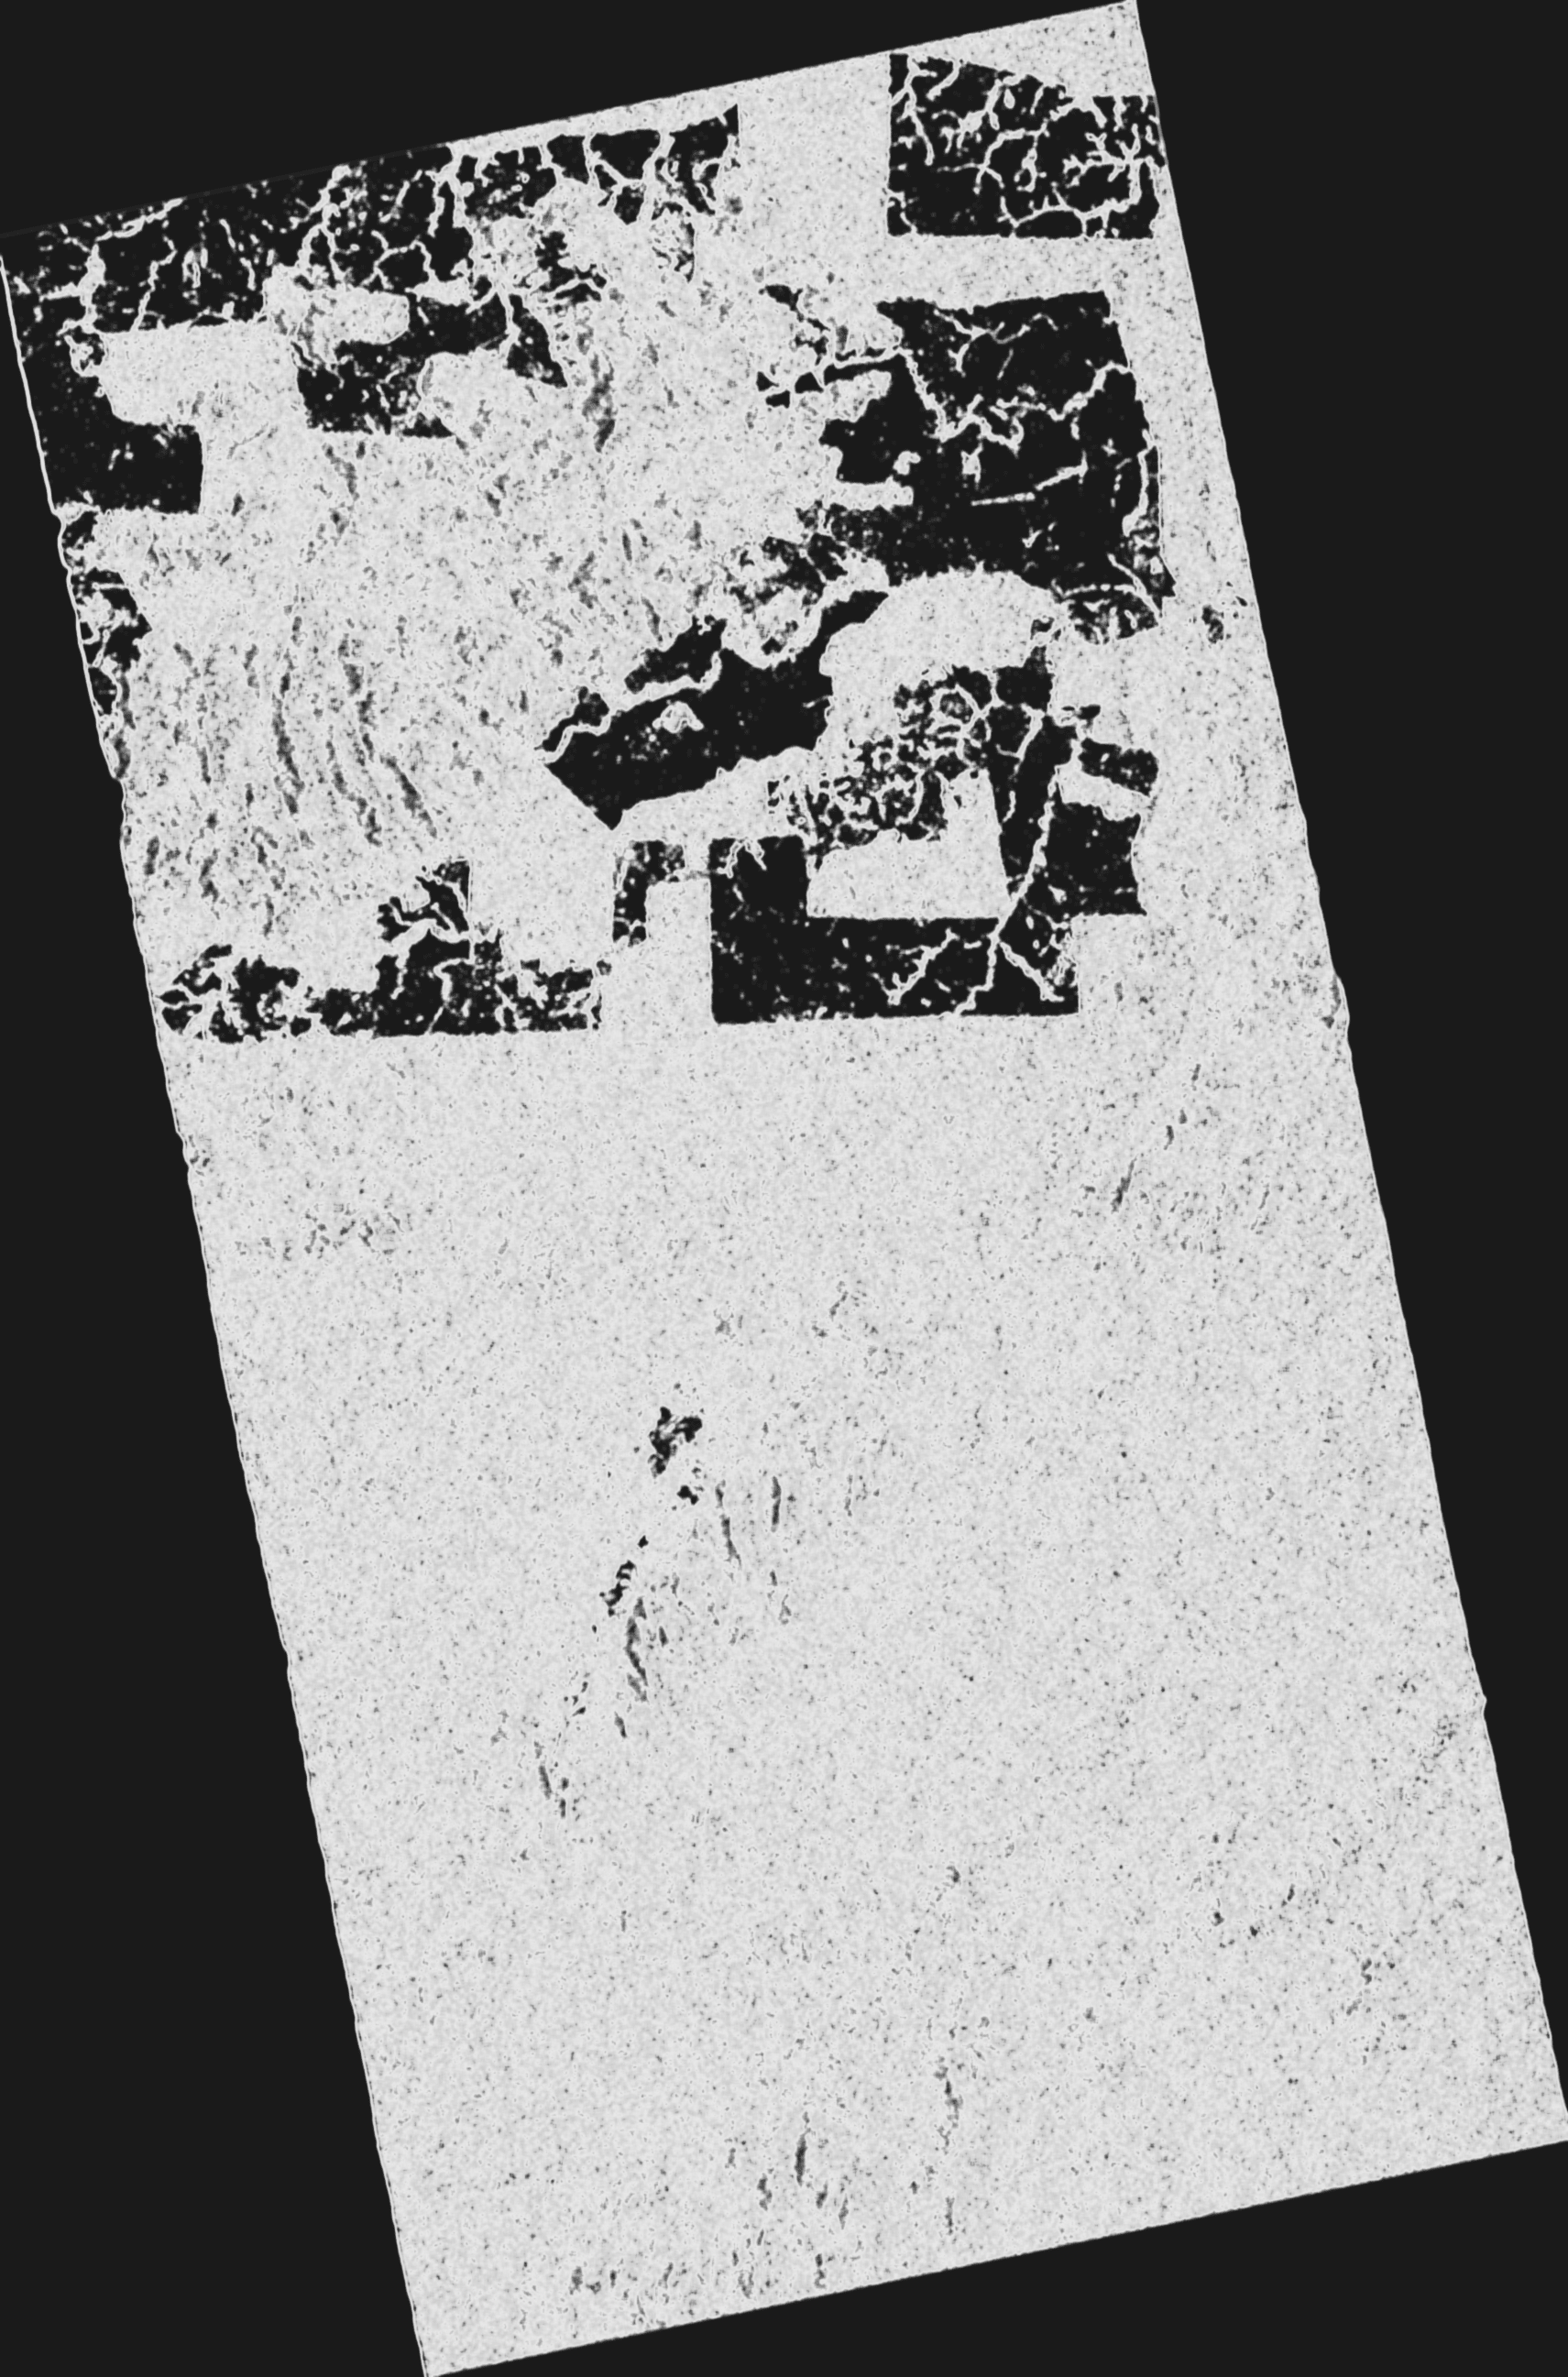
\includegraphics[width=\linewidth]{Chapter4/glcm_textures/homogeneityimage.png}
    \caption{Homogeneity texture of Coherence Image}
  \end{subfigure}
\end{figure}

Just by looking at the images above it might be hard to know if they are better suited for classification or not. One solution in order to be able to know quantitatively if they are better to classification is to look at the histogram of the pixels intensity and to compare it with the histograms of the pixels intensity for forest and non forest area in the original coherence image.
For this area it was provided the reference map for comparison, so it is know if a pixel is in a forest area or in a deforested area, and by using this reference map it is possible to make the histograms of the pixel intensity for each area and to compare it with the original histograms for the coherence.
\begin{figure}[H]
  \centering
  \begin{subfigure}[b]{0.4\linewidth}
    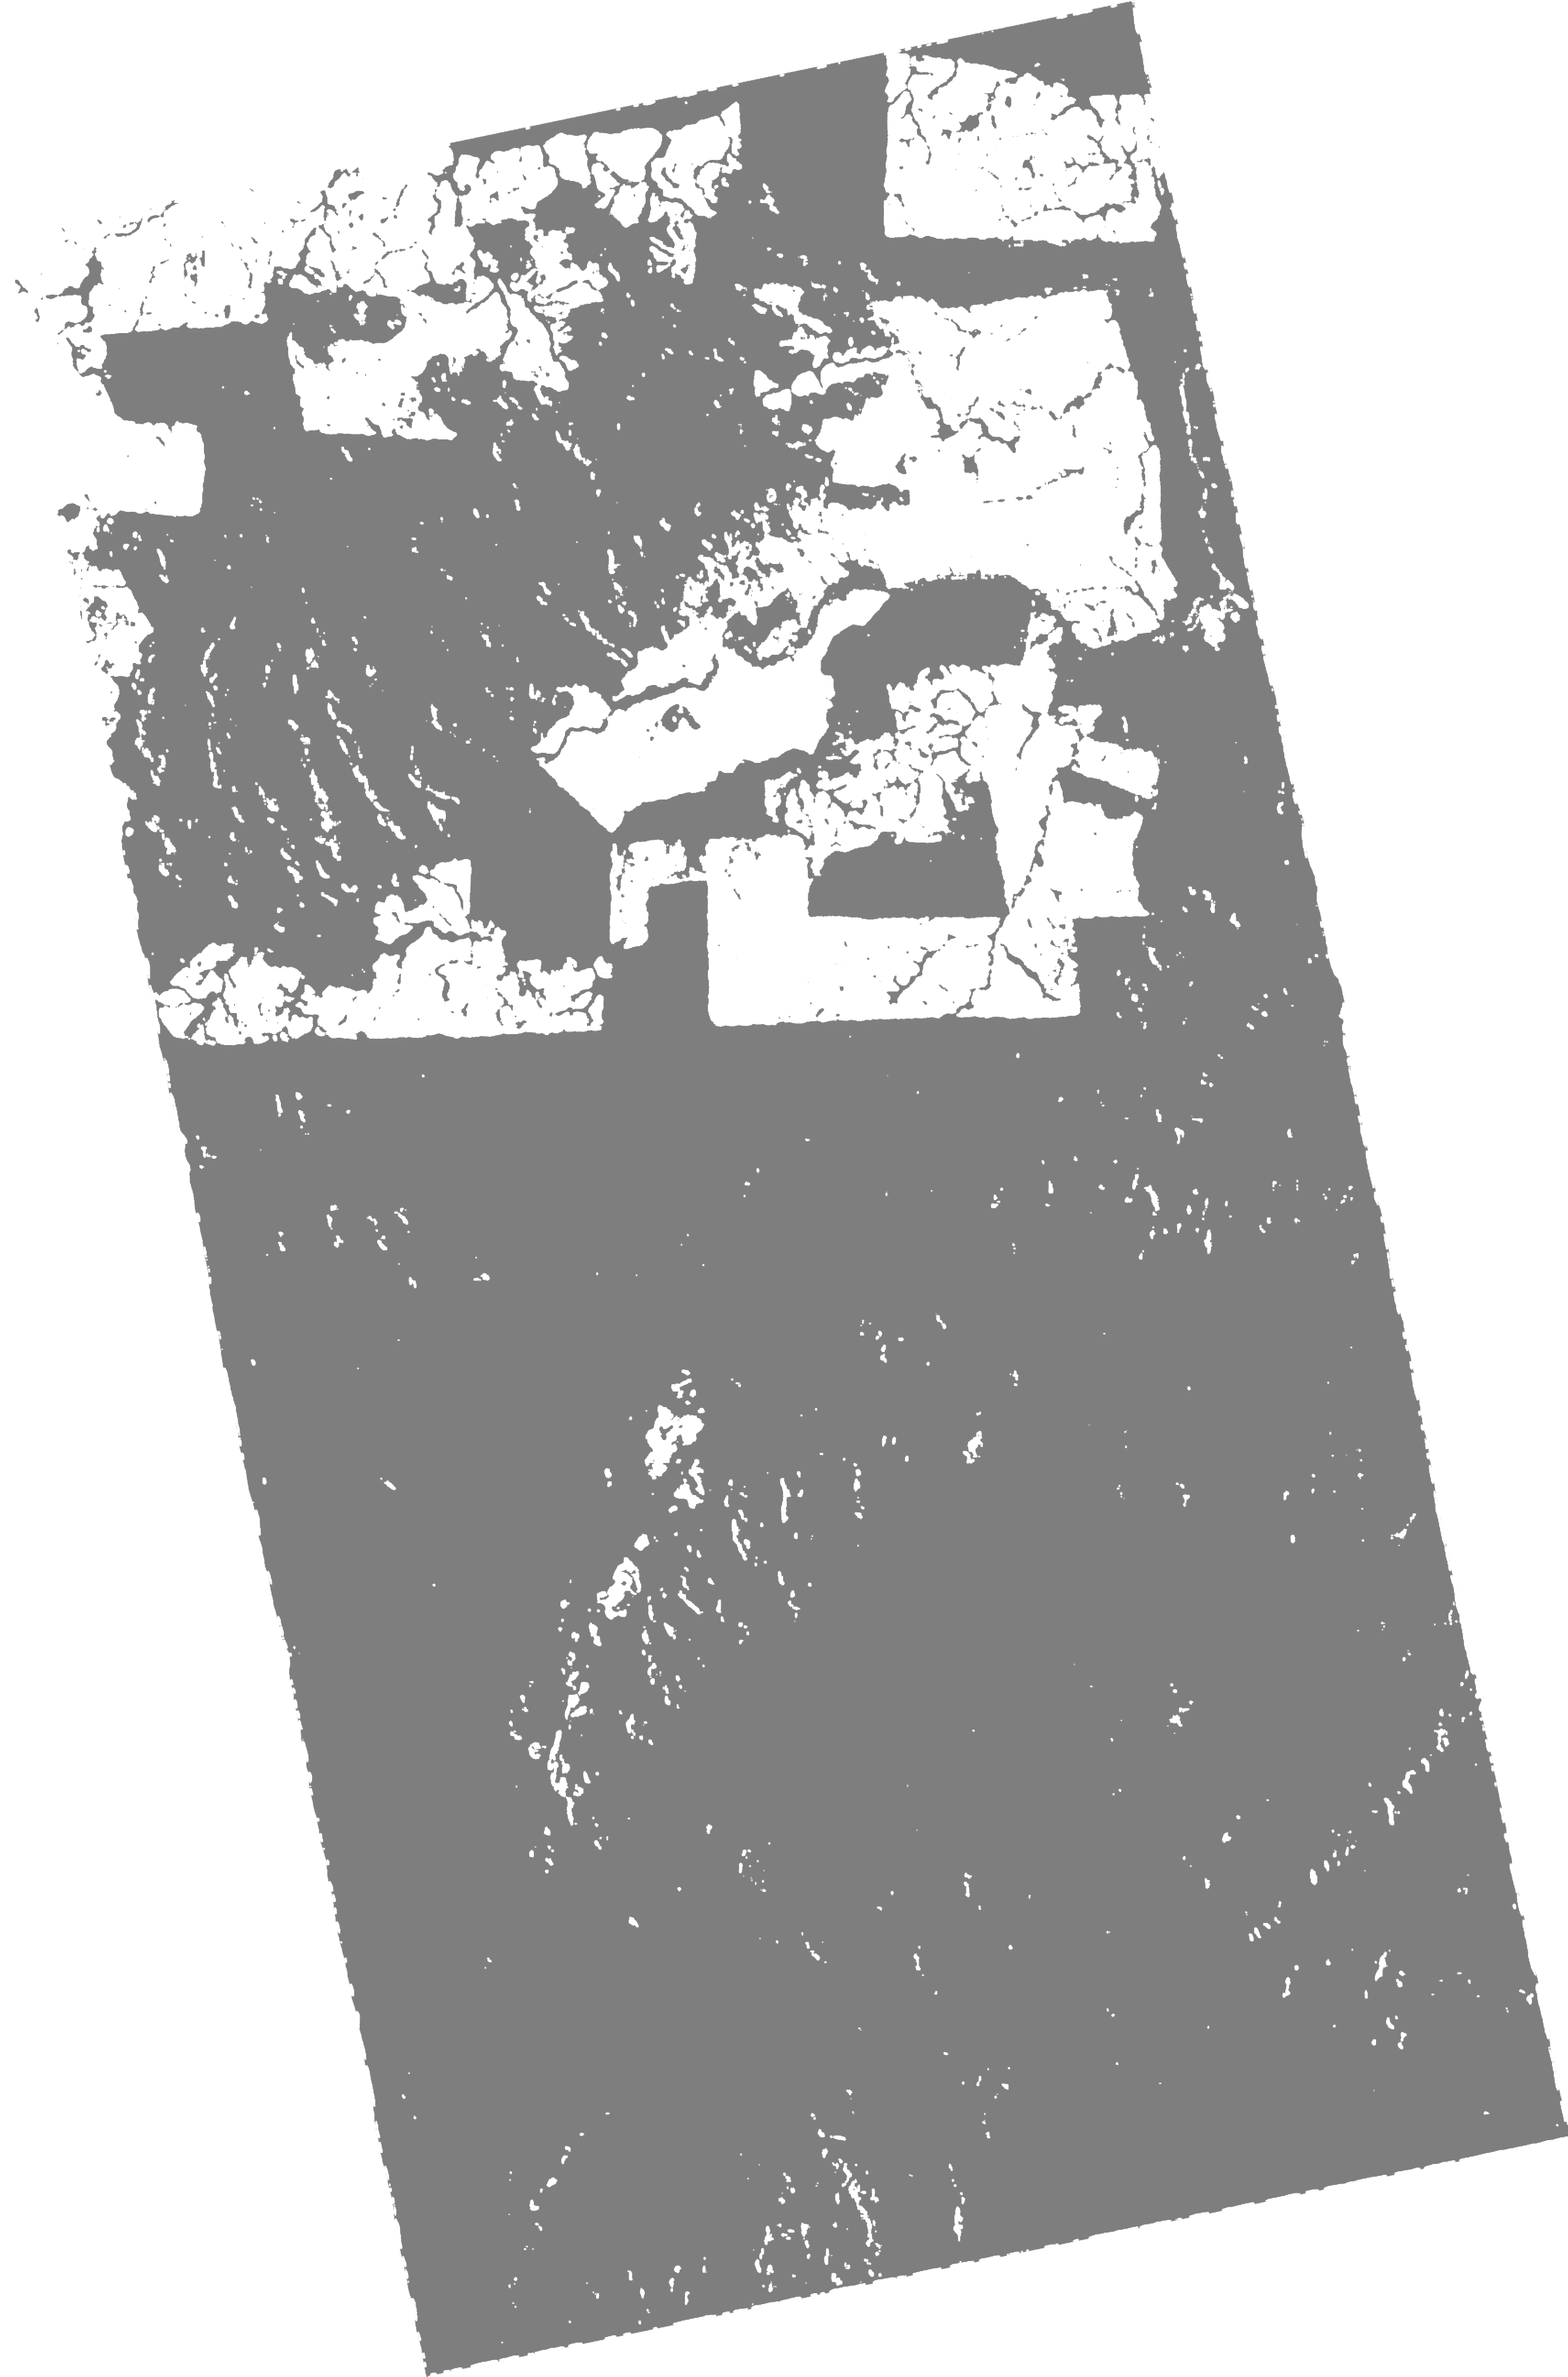
\includegraphics[width=\linewidth]{Chapter4/referencemap.png}
     
  \end{subfigure}
  \caption{Reference Map provided by DLR.}
  \label{fig:reference_map}
\end{figure}
From the reference map above it was possible to extract the following probability density function from the histogram of the coherence.
\begin{figure}[H]
  \centering
  \begin{subfigure}[b]{\linewidth}
    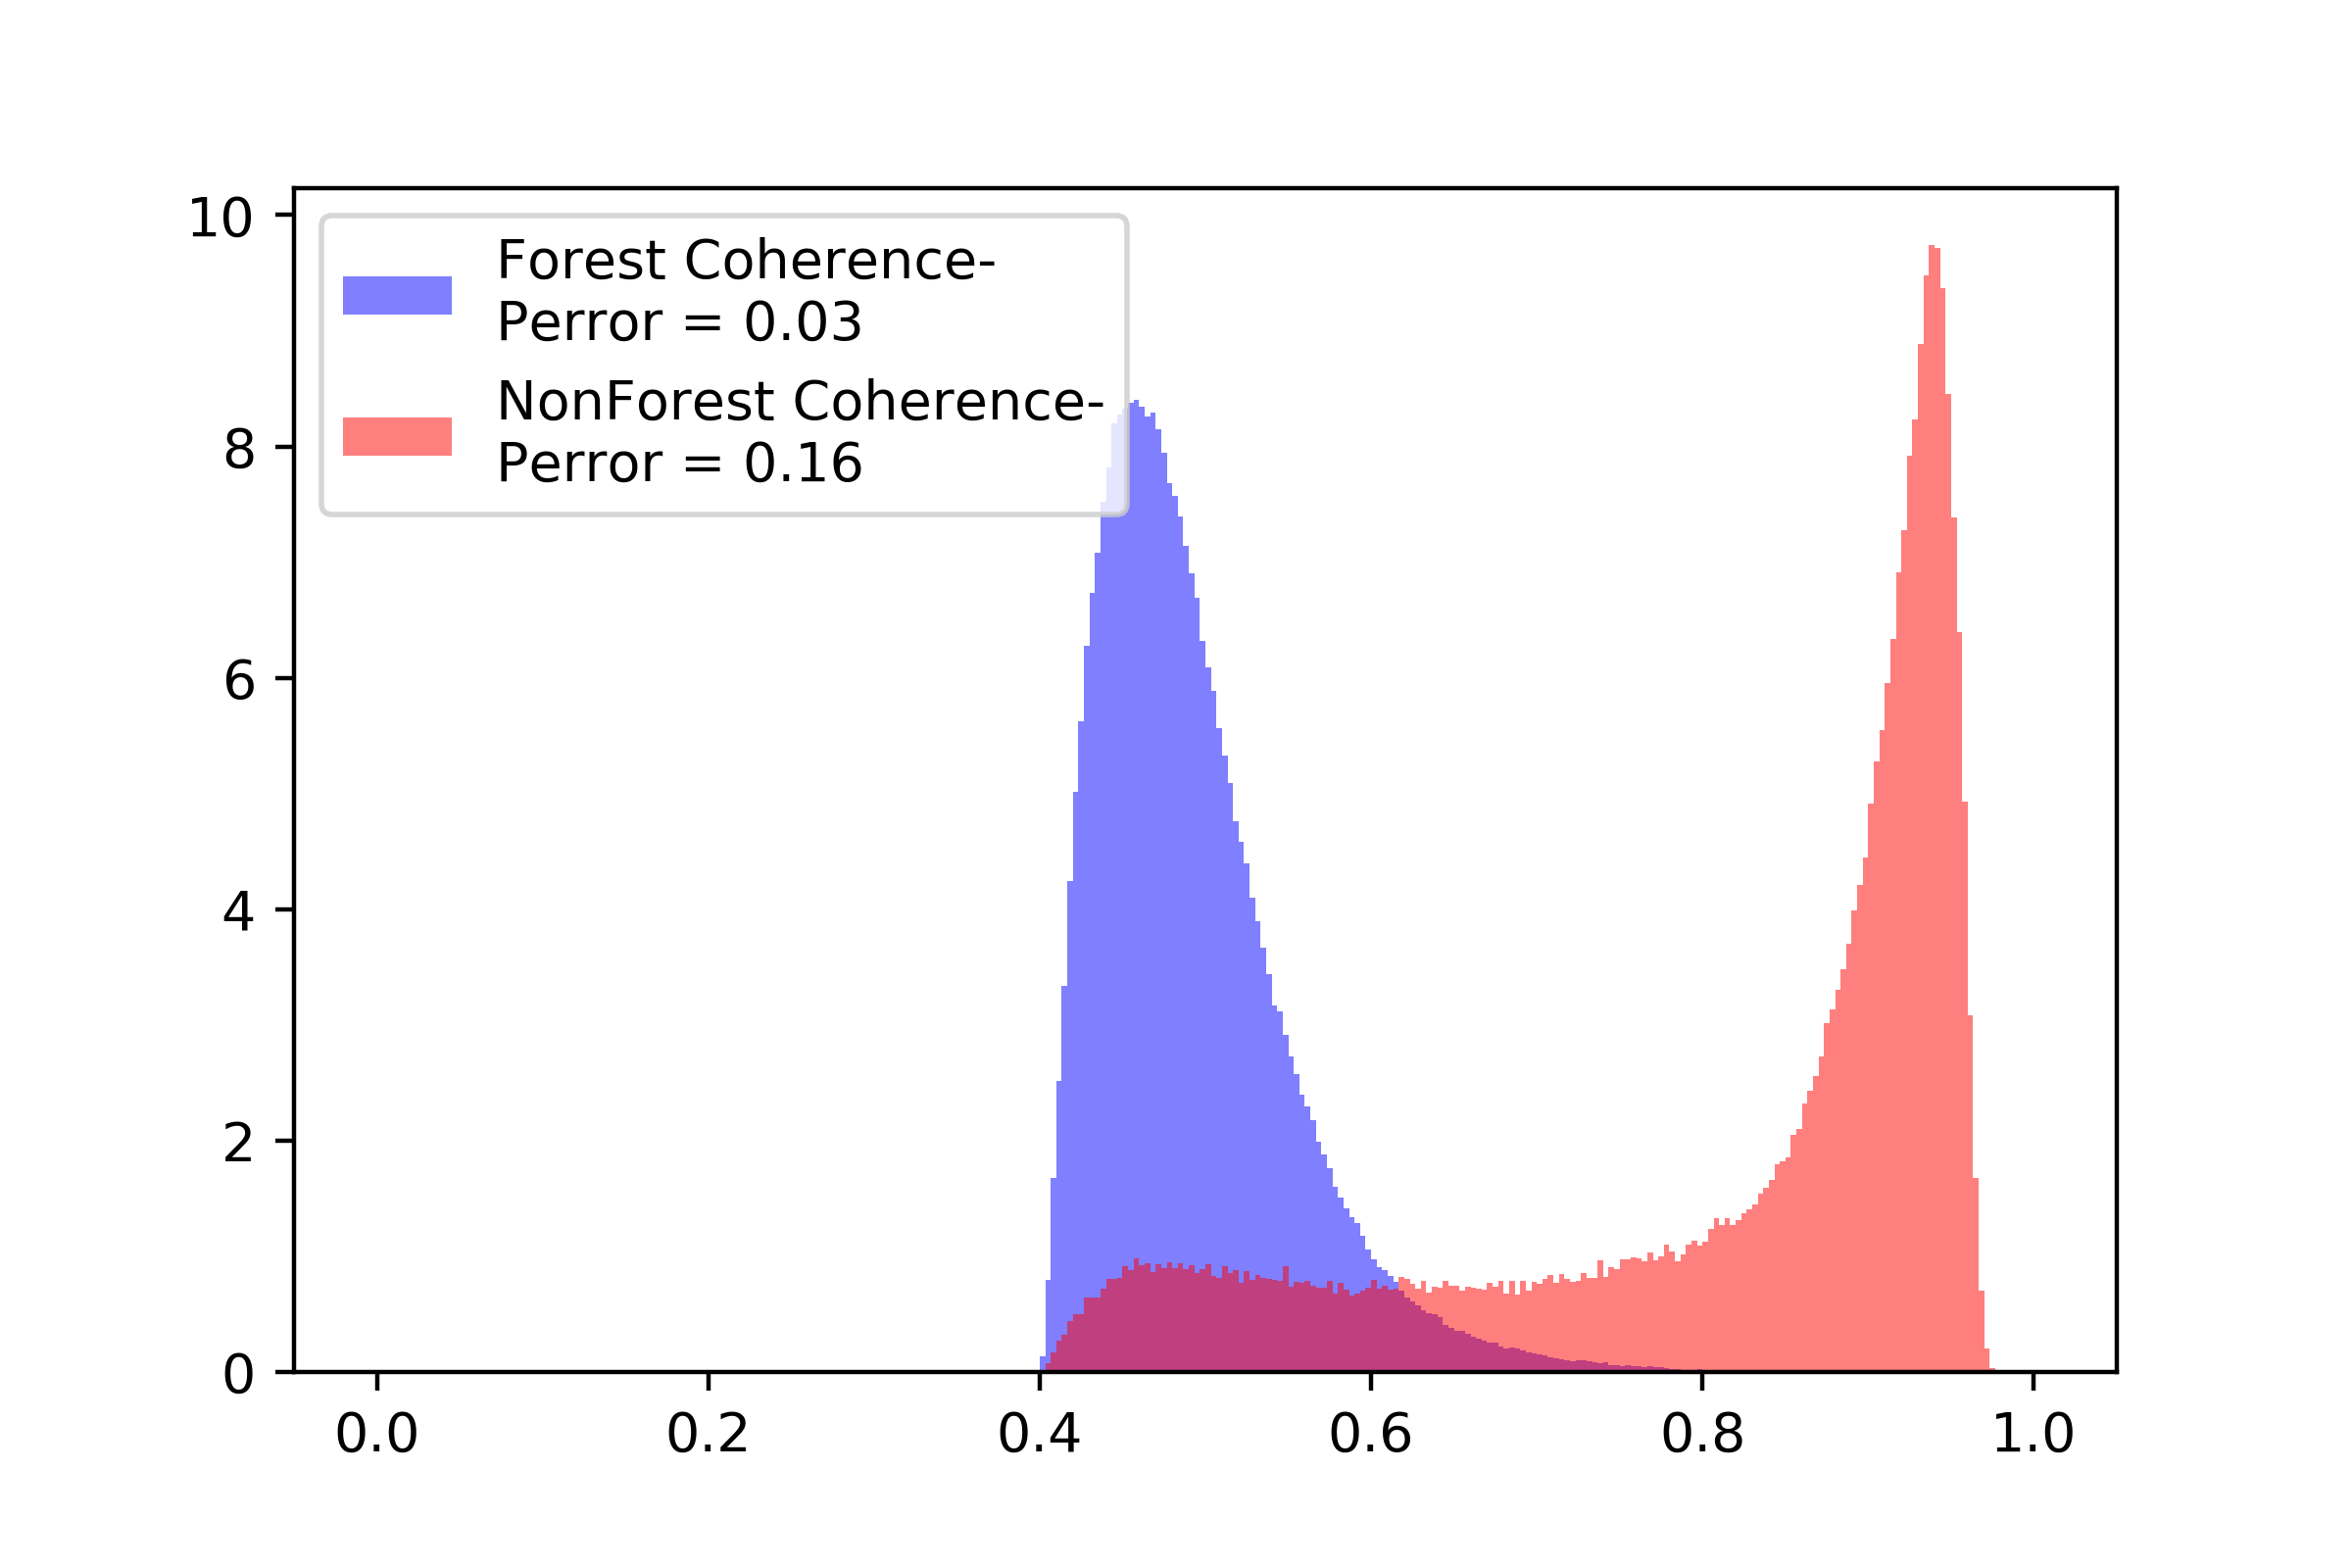
\includegraphics[width=\linewidth]{Chapter4/histogramcoherence.png}
     \caption{Probability density Function for Coherence.}
  \end{subfigure}
\end{figure}
It is possible to see that the probability density functions (PDF) overlap at some point, which implies that there is always a probability of error when trying to classify the information of the pixel. On the image above it was also calculated which percentage of the area of one PDF is below the other PDF. For example, from the image above, 3 percent of the forest coherence PDF was below the Non Forest coherence PDF while 16 percent of the non forest coherence PDF was below the forest coherence PDF.
We can see the PDFs obtained from the histograms of the texture features and see whether the PDFs are more separated compared to the PDFs of the coherence.

\begin{figure}[H]
  \centering
  \begin{subfigure}[b]{0.4\linewidth}
    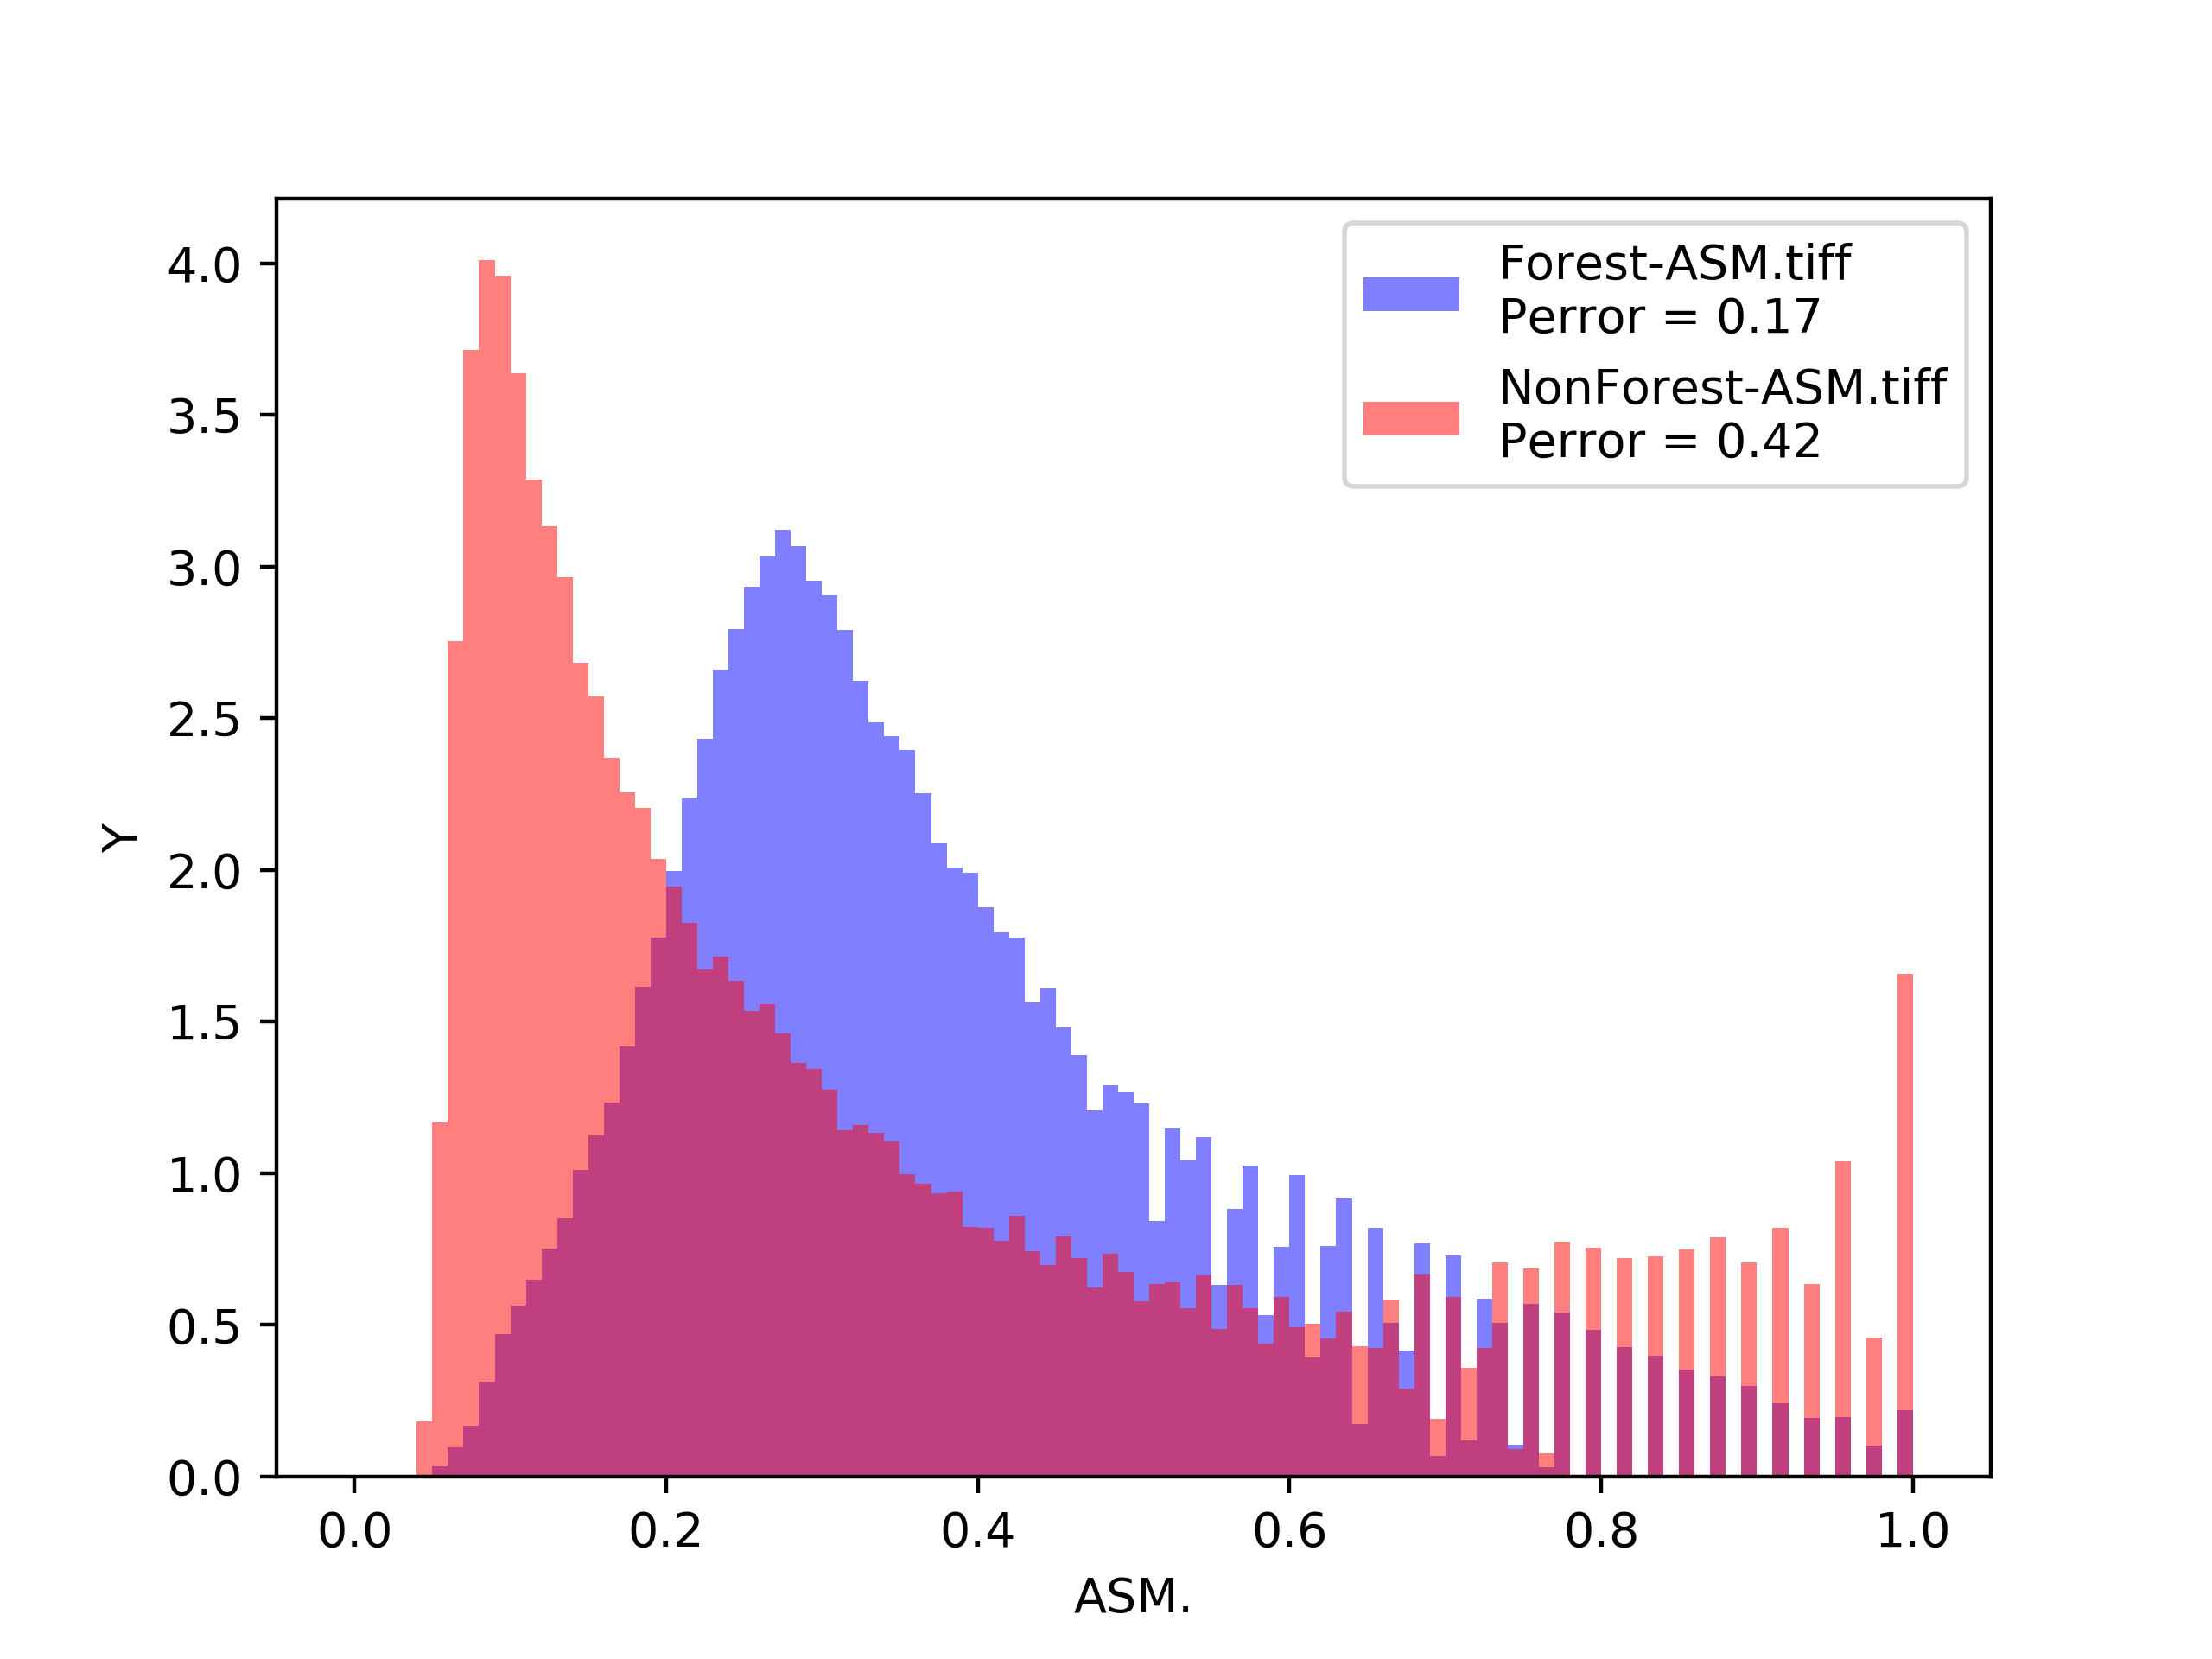
\includegraphics[width=\linewidth]{Chapter4/glcm_textures/ASM_hist.png}
     \caption{Probability density Function for Angular Second Moment.}
  \end{subfigure}
  \centering
  \begin{subfigure}[b]{0.4\linewidth}
    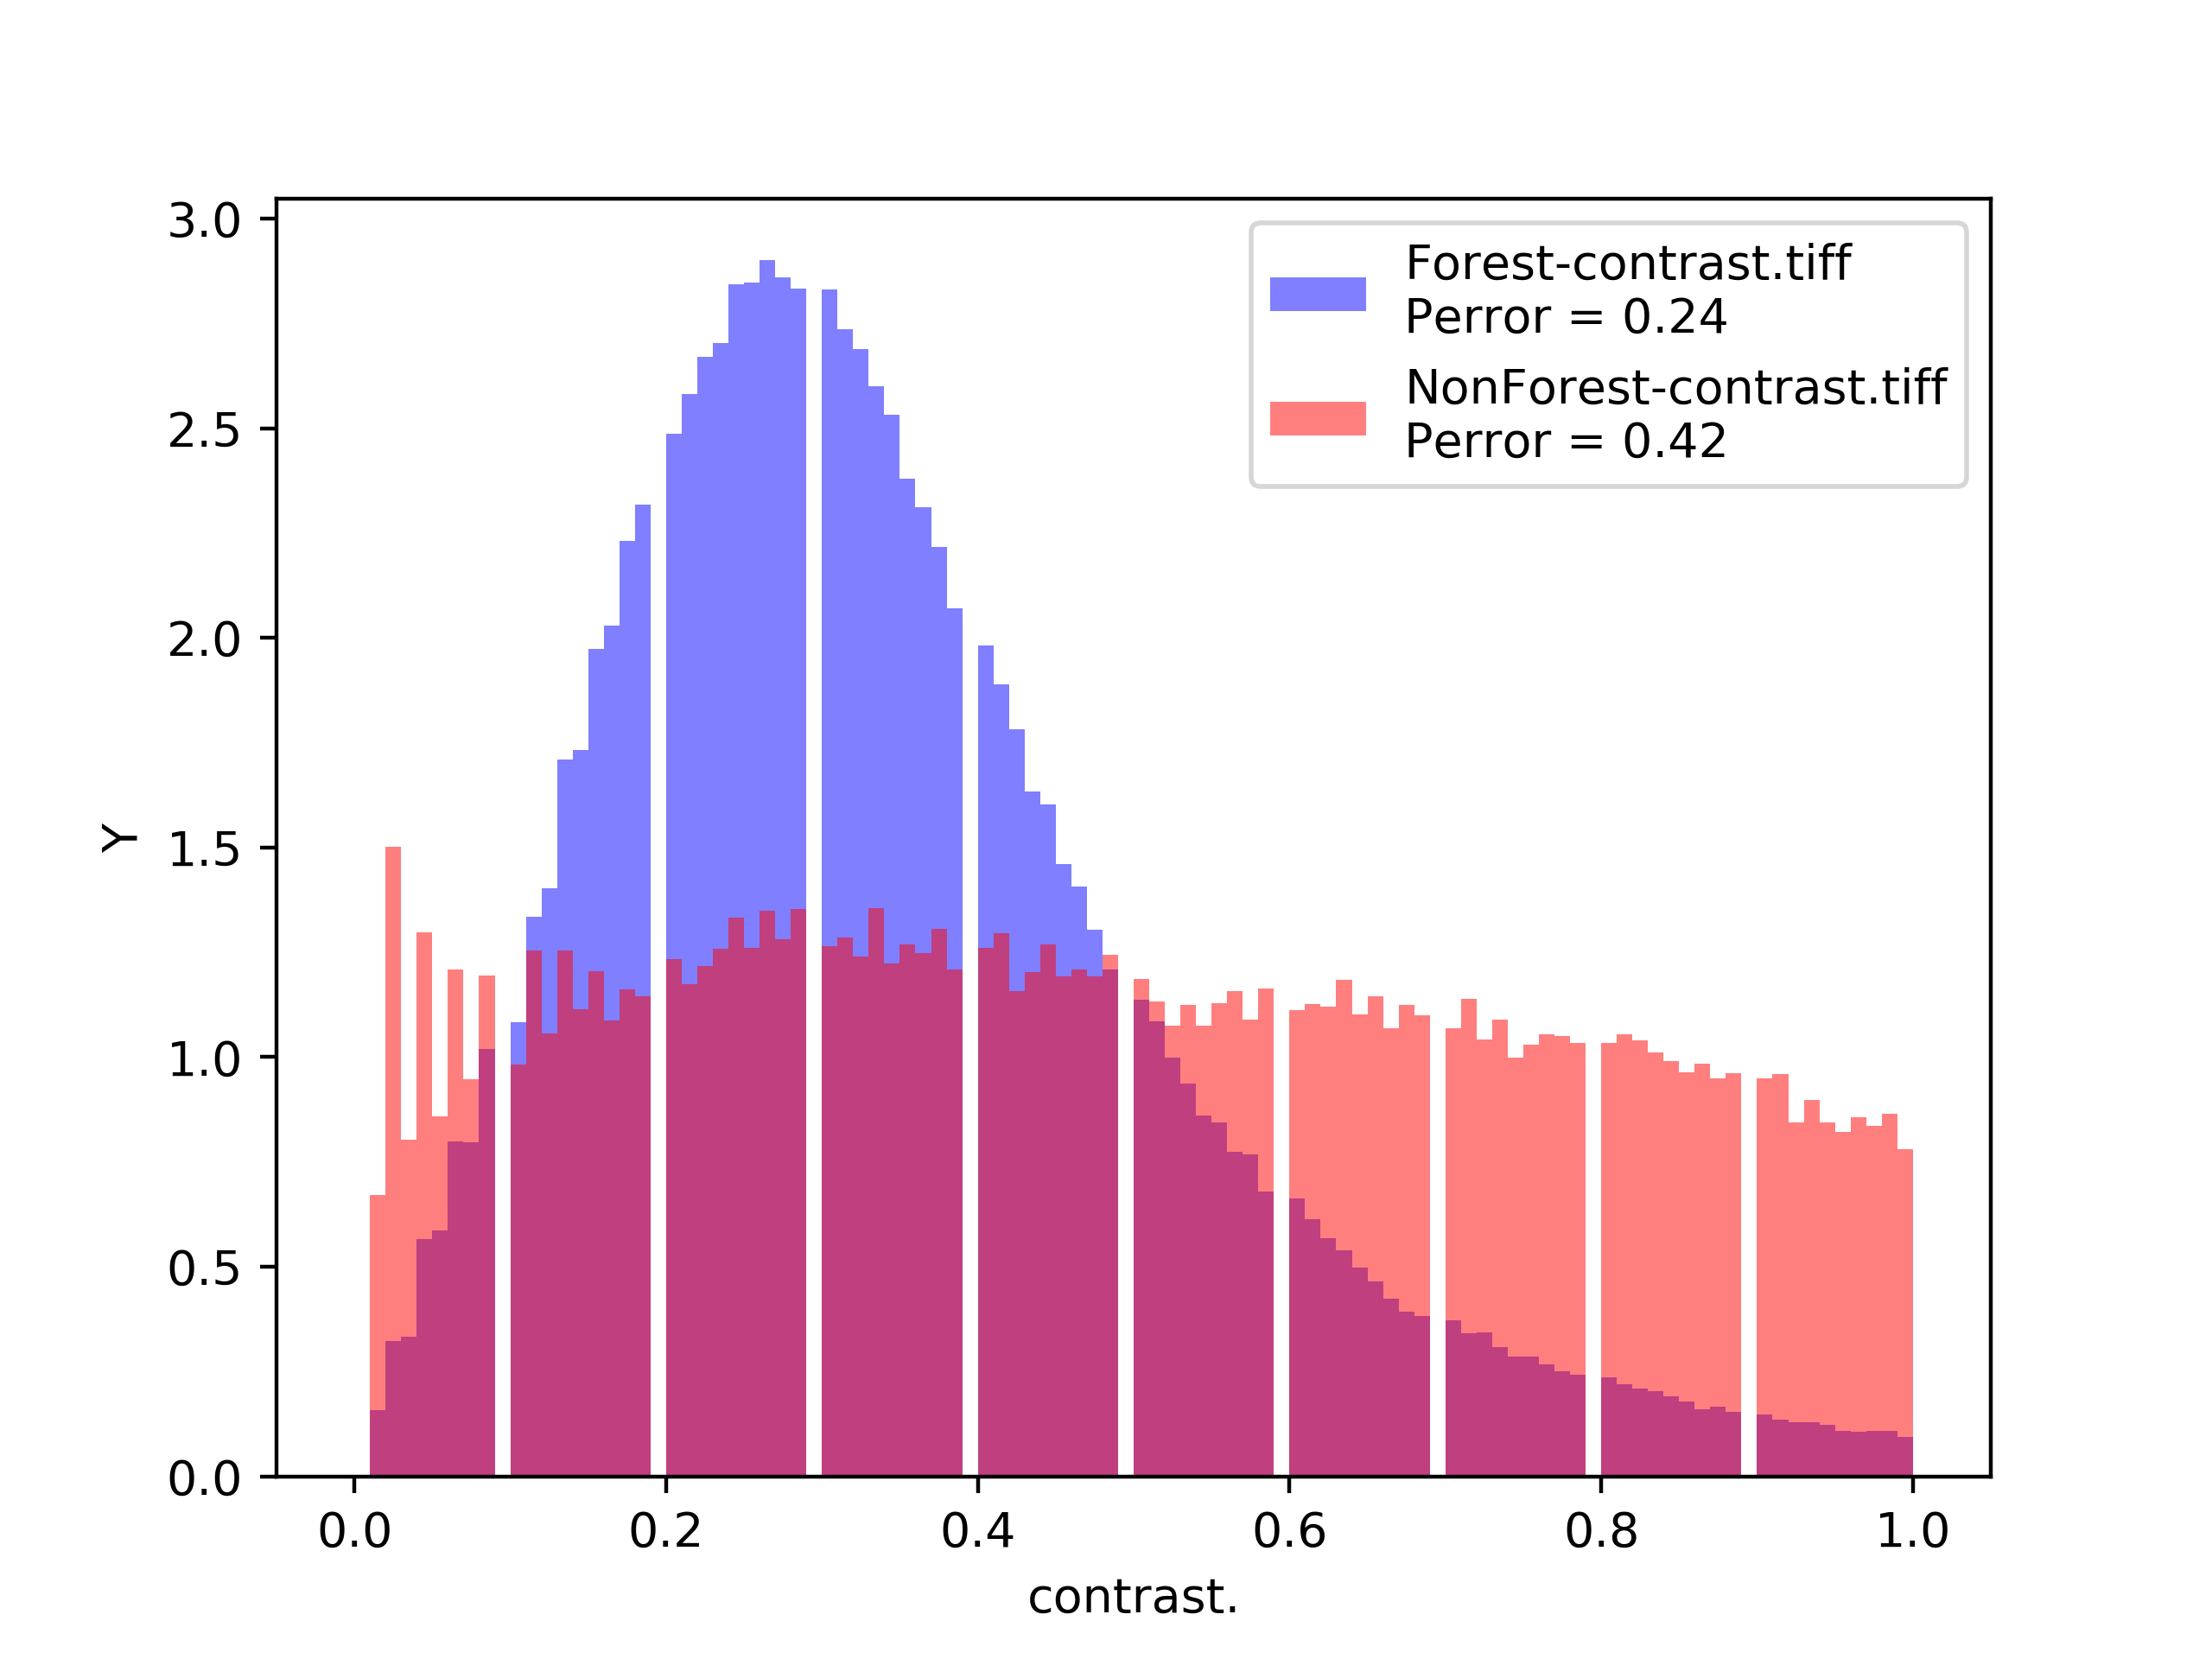
\includegraphics[width=\linewidth]{Chapter4/glcm_textures/contrast_hist.png}
     \caption{Probability density Function for Contrast.}
  \end{subfigure}
  \centering
  \begin{subfigure}[b]{0.4\linewidth}
    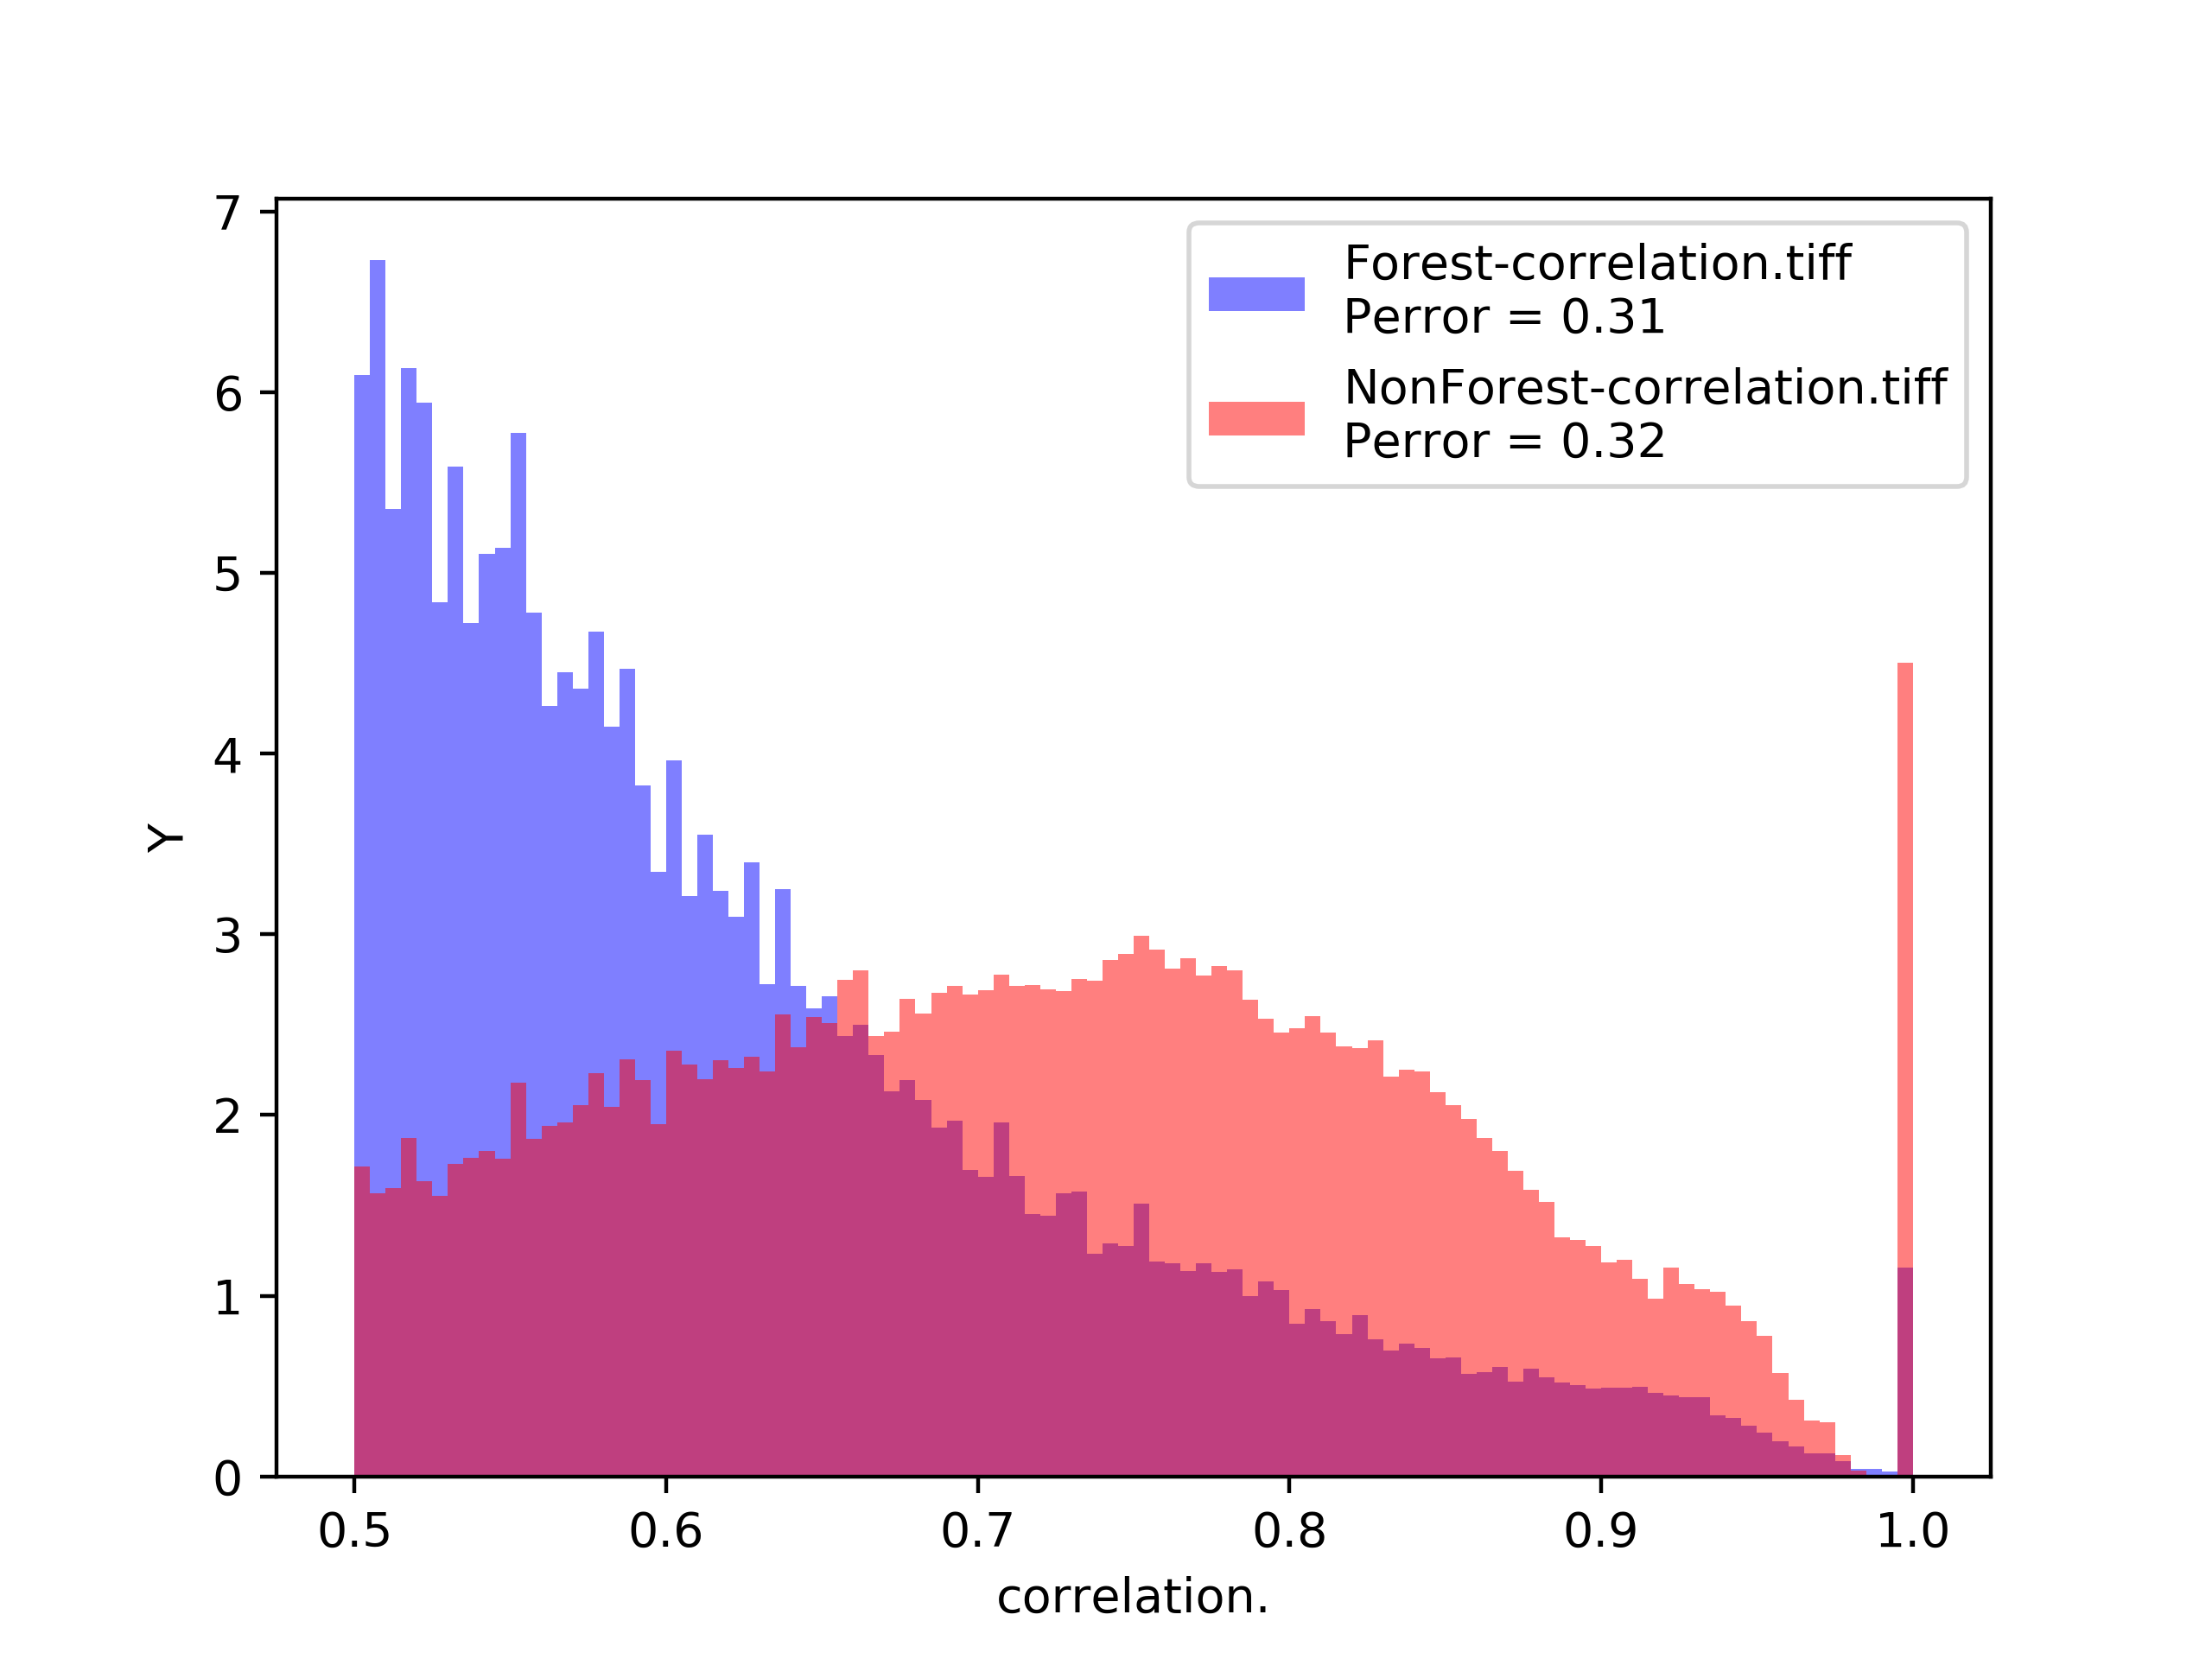
\includegraphics[width=\linewidth]{Chapter4/glcm_textures/correlation_hist.png}
     \caption{Probability density Function for Correlation.}
  \end{subfigure}
  \centering
  \begin{subfigure}[b]{0.4\linewidth}
    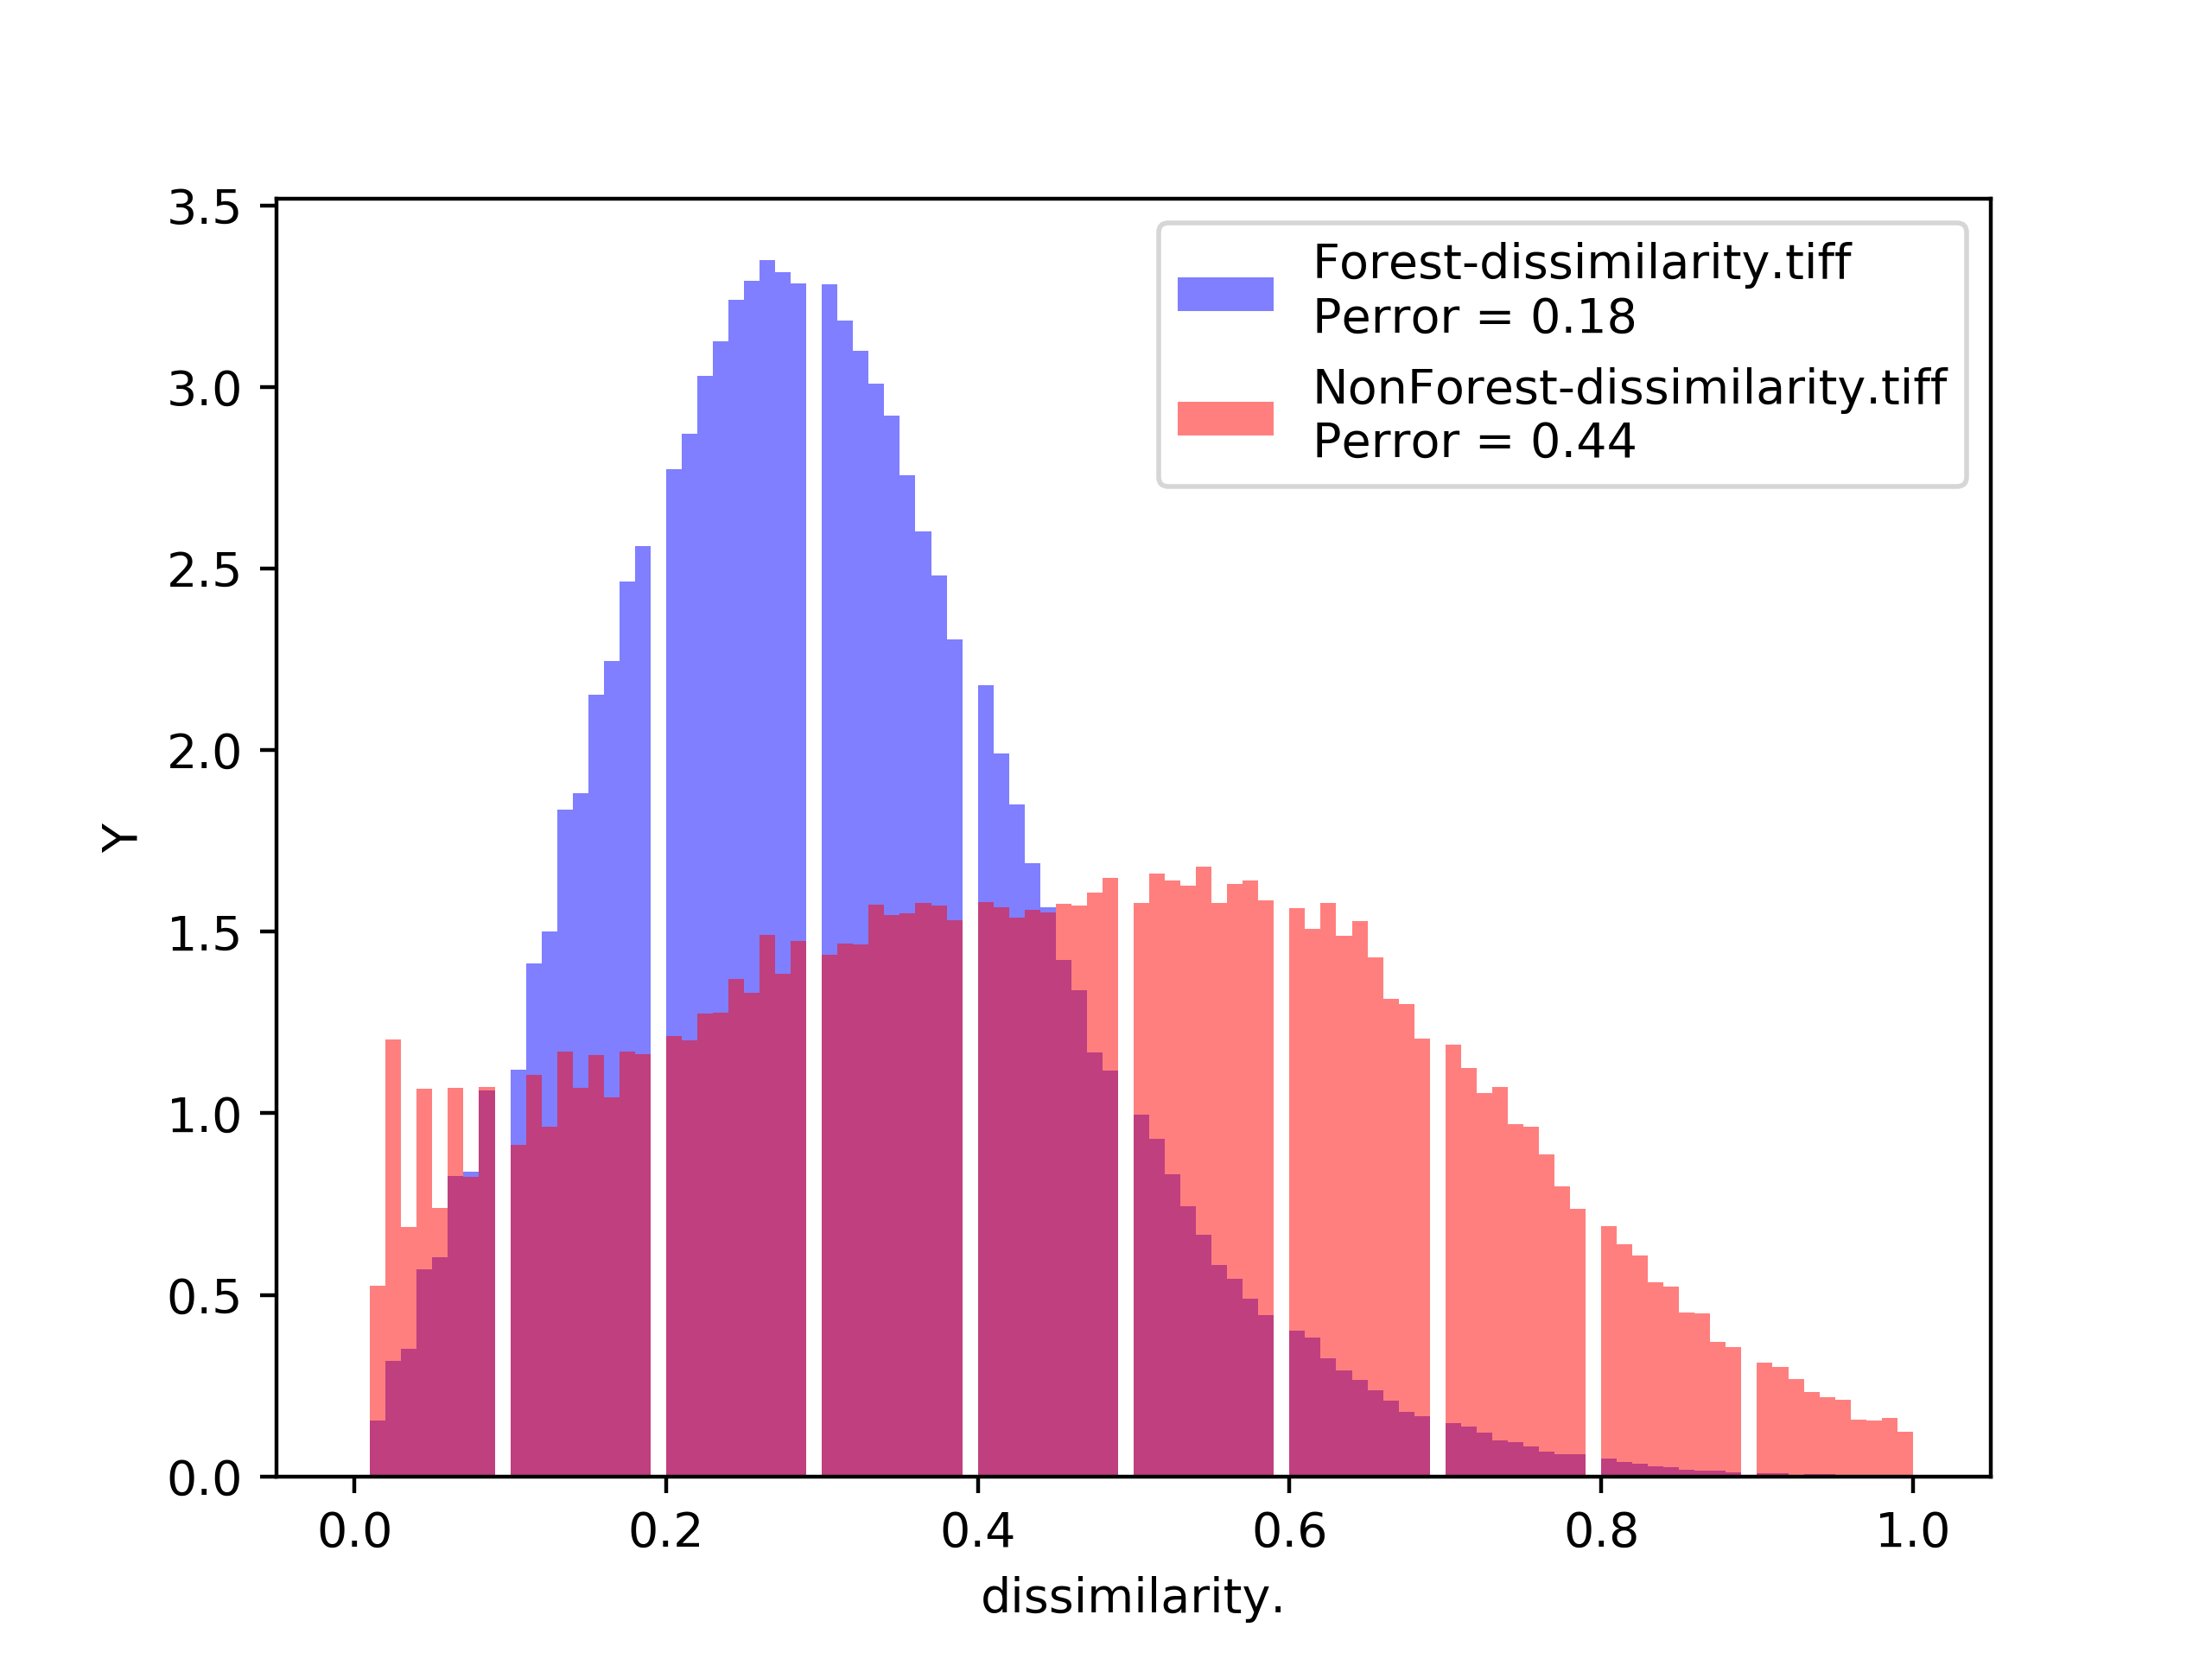
\includegraphics[width=\linewidth]{Chapter4/glcm_textures/dissimilarity_hist.png}
     \caption{Probability density Function for Dissimilarity.}
  \end{subfigure}
  \centering
  \begin{subfigure}[b]{0.4\linewidth}
    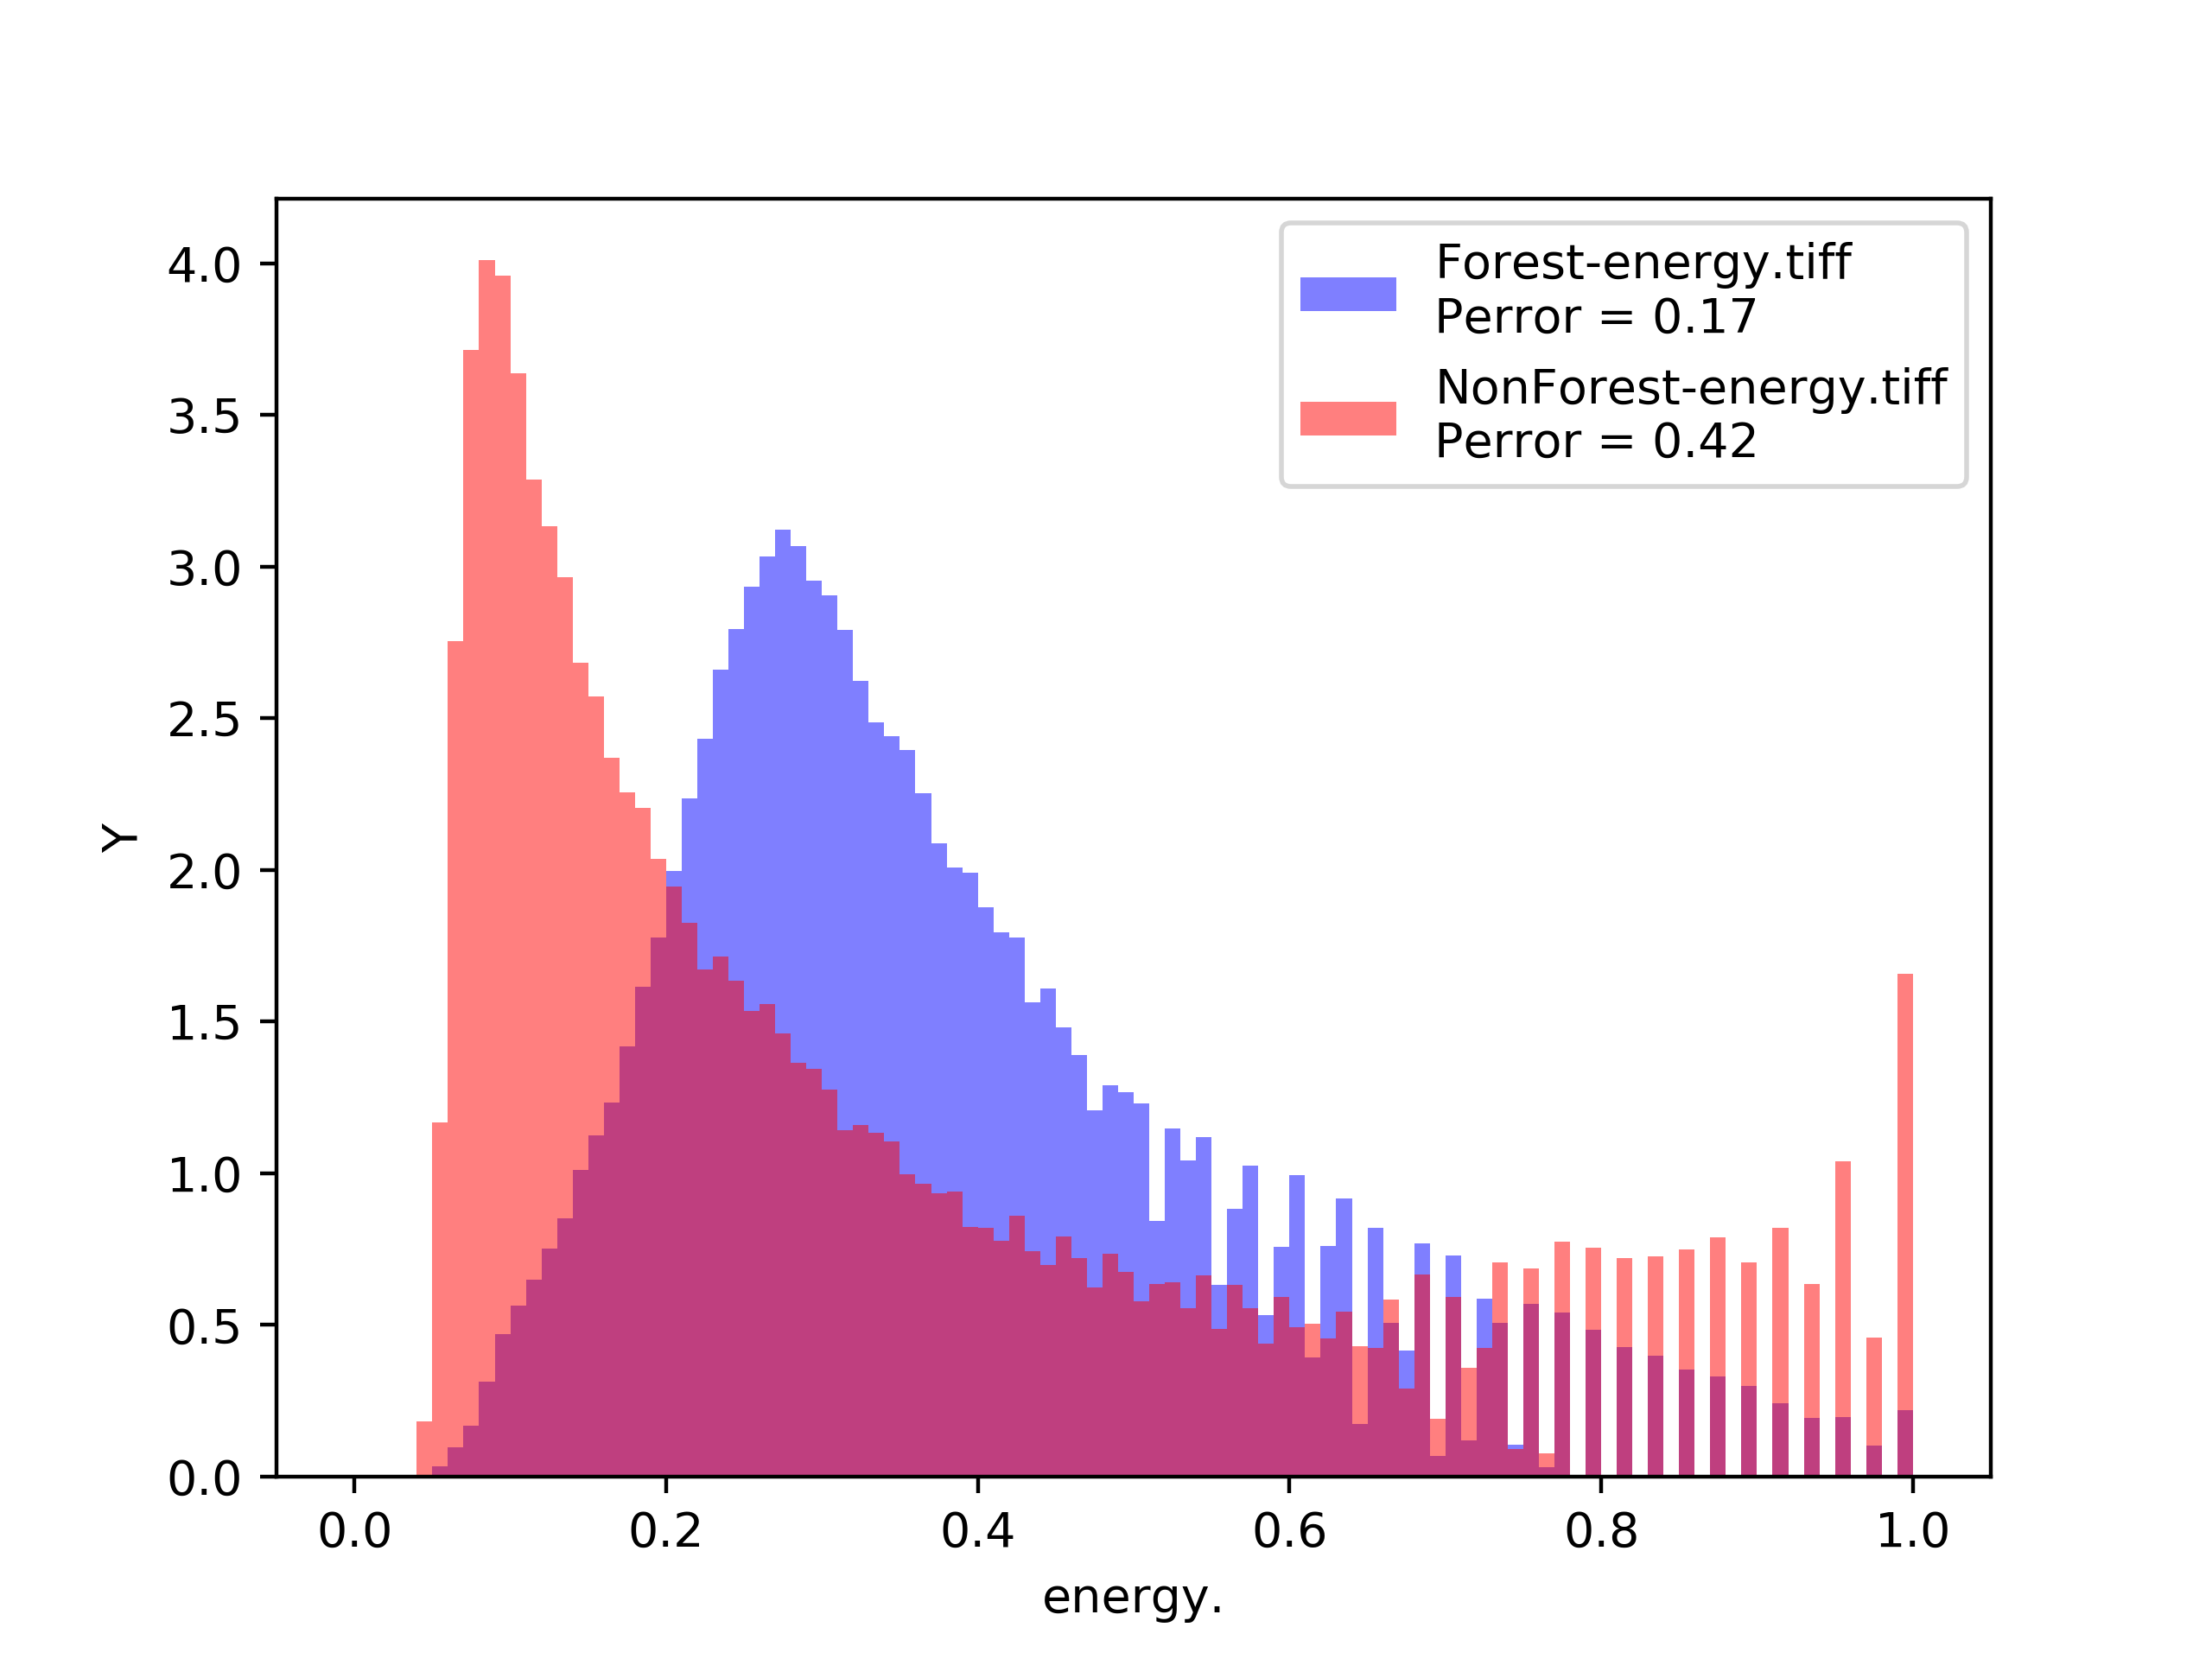
\includegraphics[width=\linewidth]{Chapter4/glcm_textures/energy_hist.png}
     \caption{Probability density Function for Energy.}
  \end{subfigure}
  \centering
  \begin{subfigure}[b]{0.4\linewidth}
    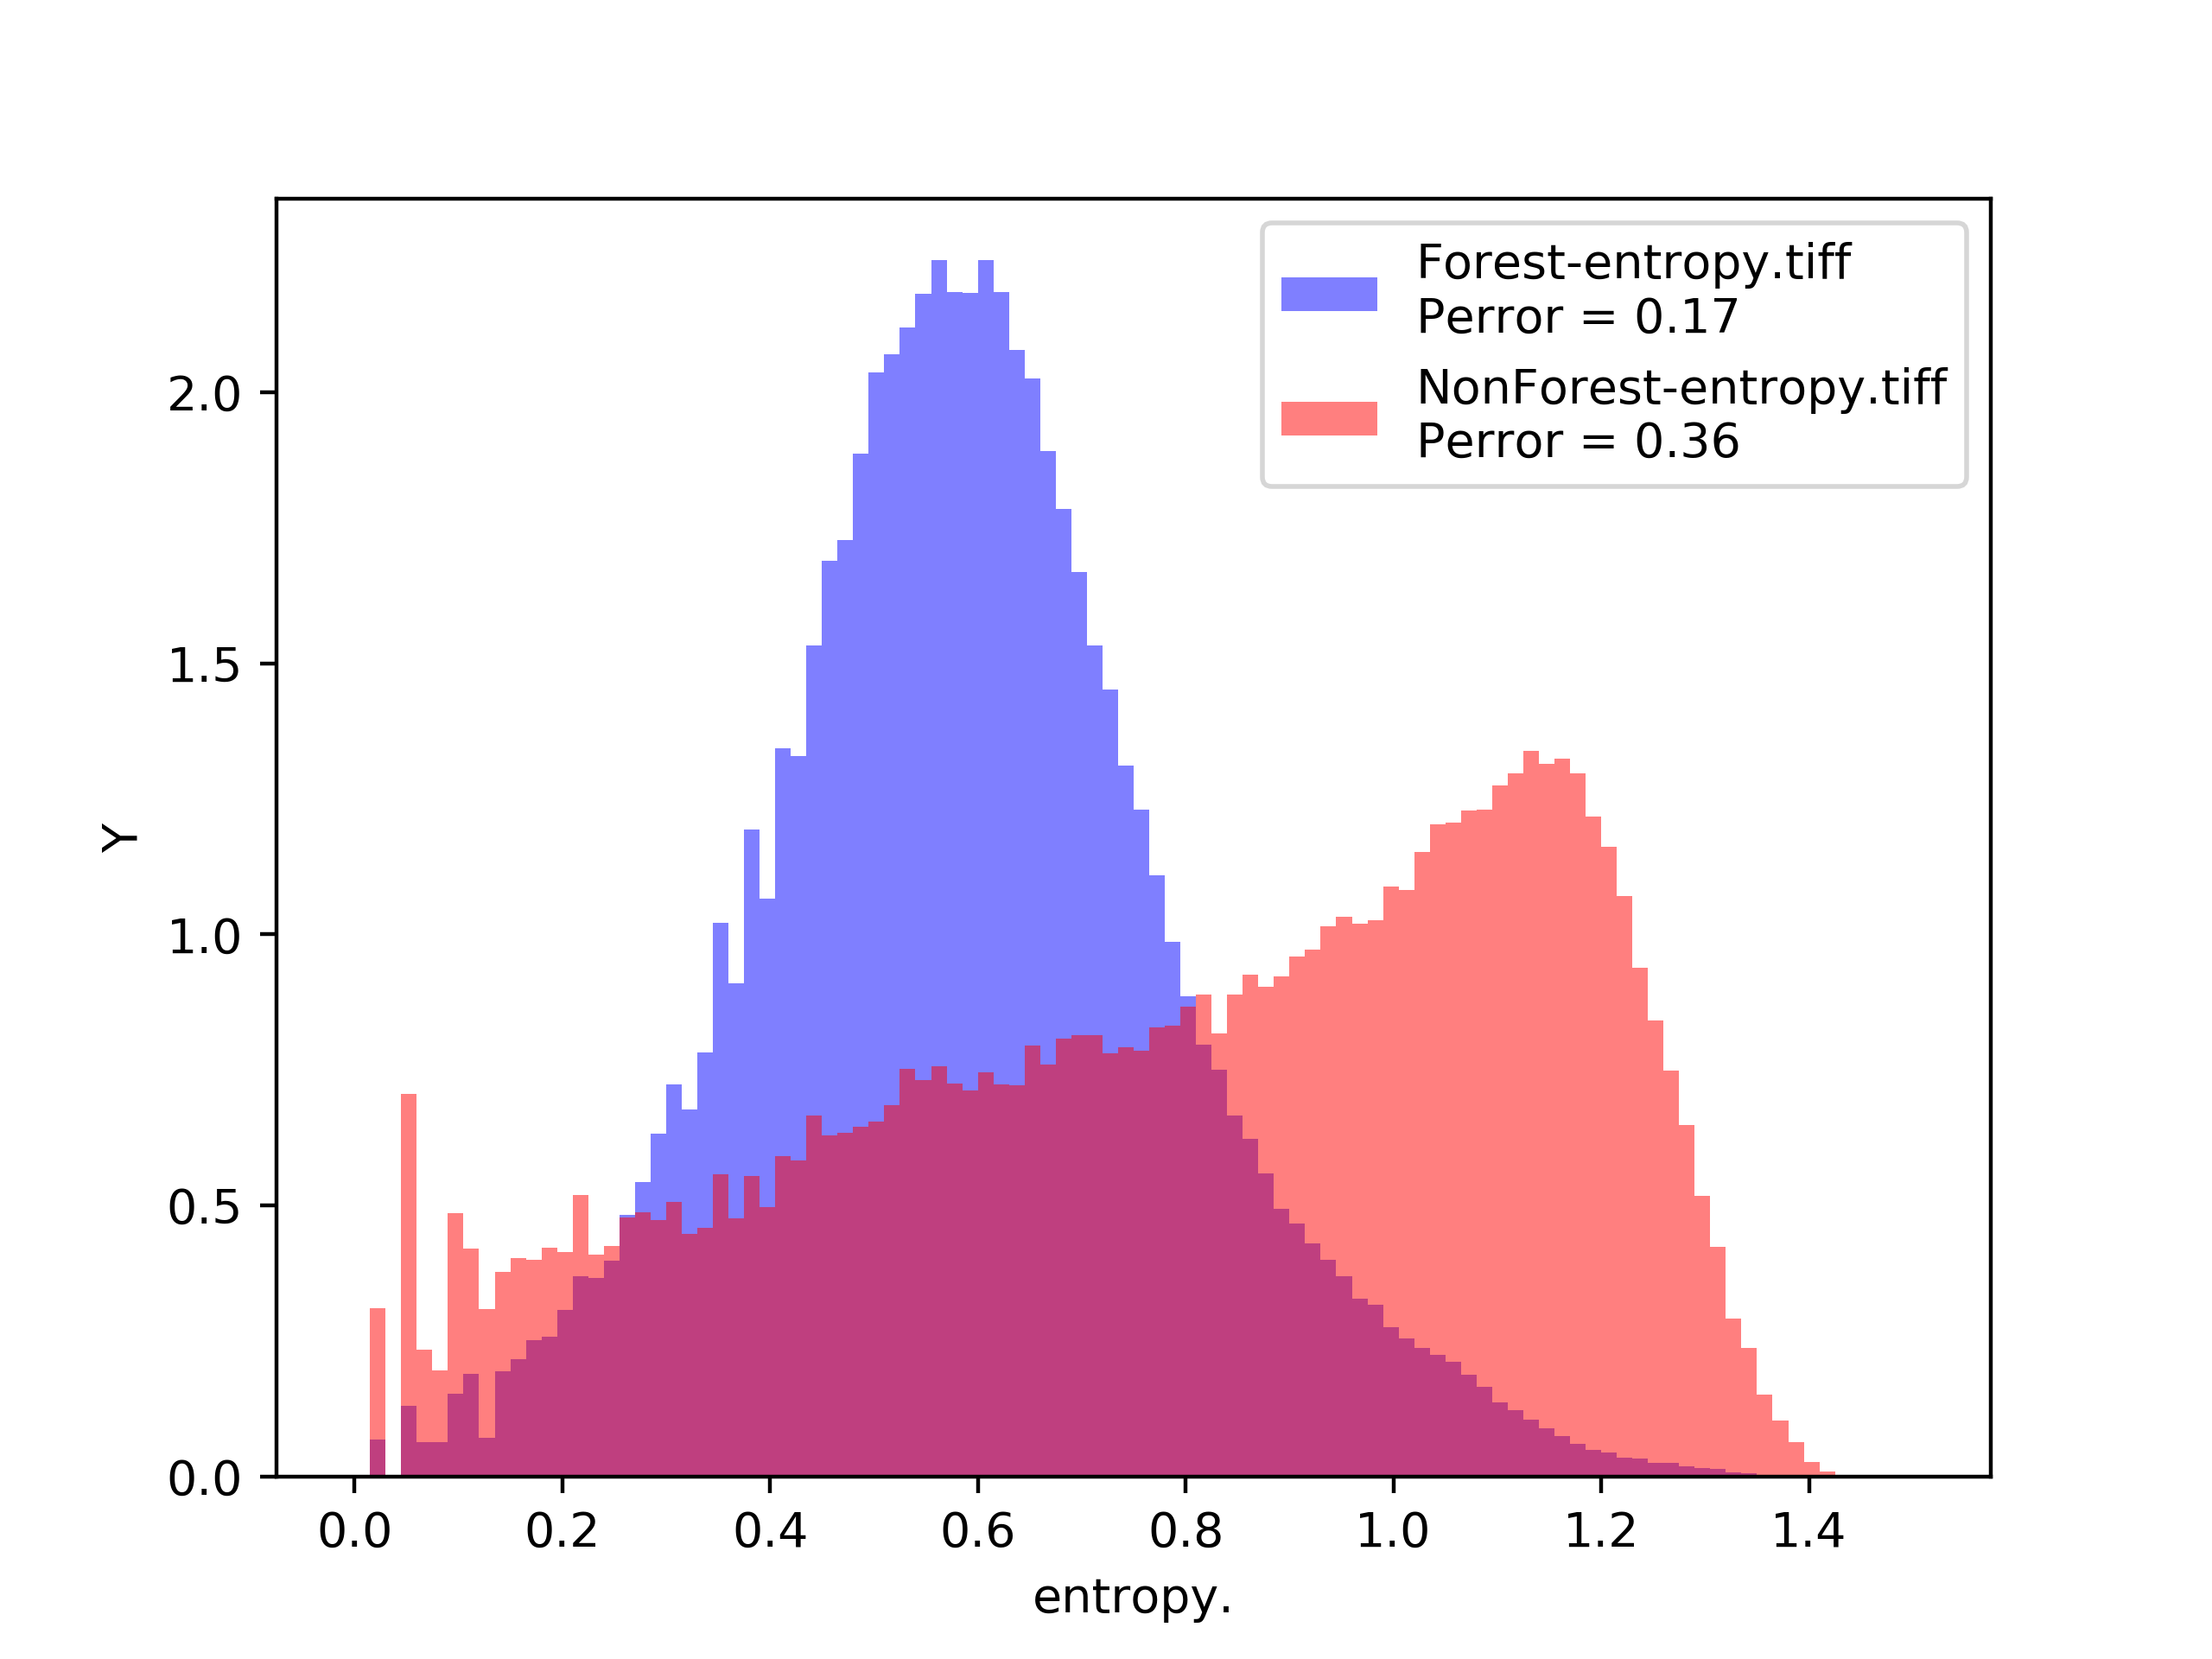
\includegraphics[width=\linewidth]{Chapter4/glcm_textures/entropy_hist.png}
     \caption{Probability density Function for Entropy.}
  \end{subfigure}
  \centering
  \begin{subfigure}[b]{0.4\linewidth}
    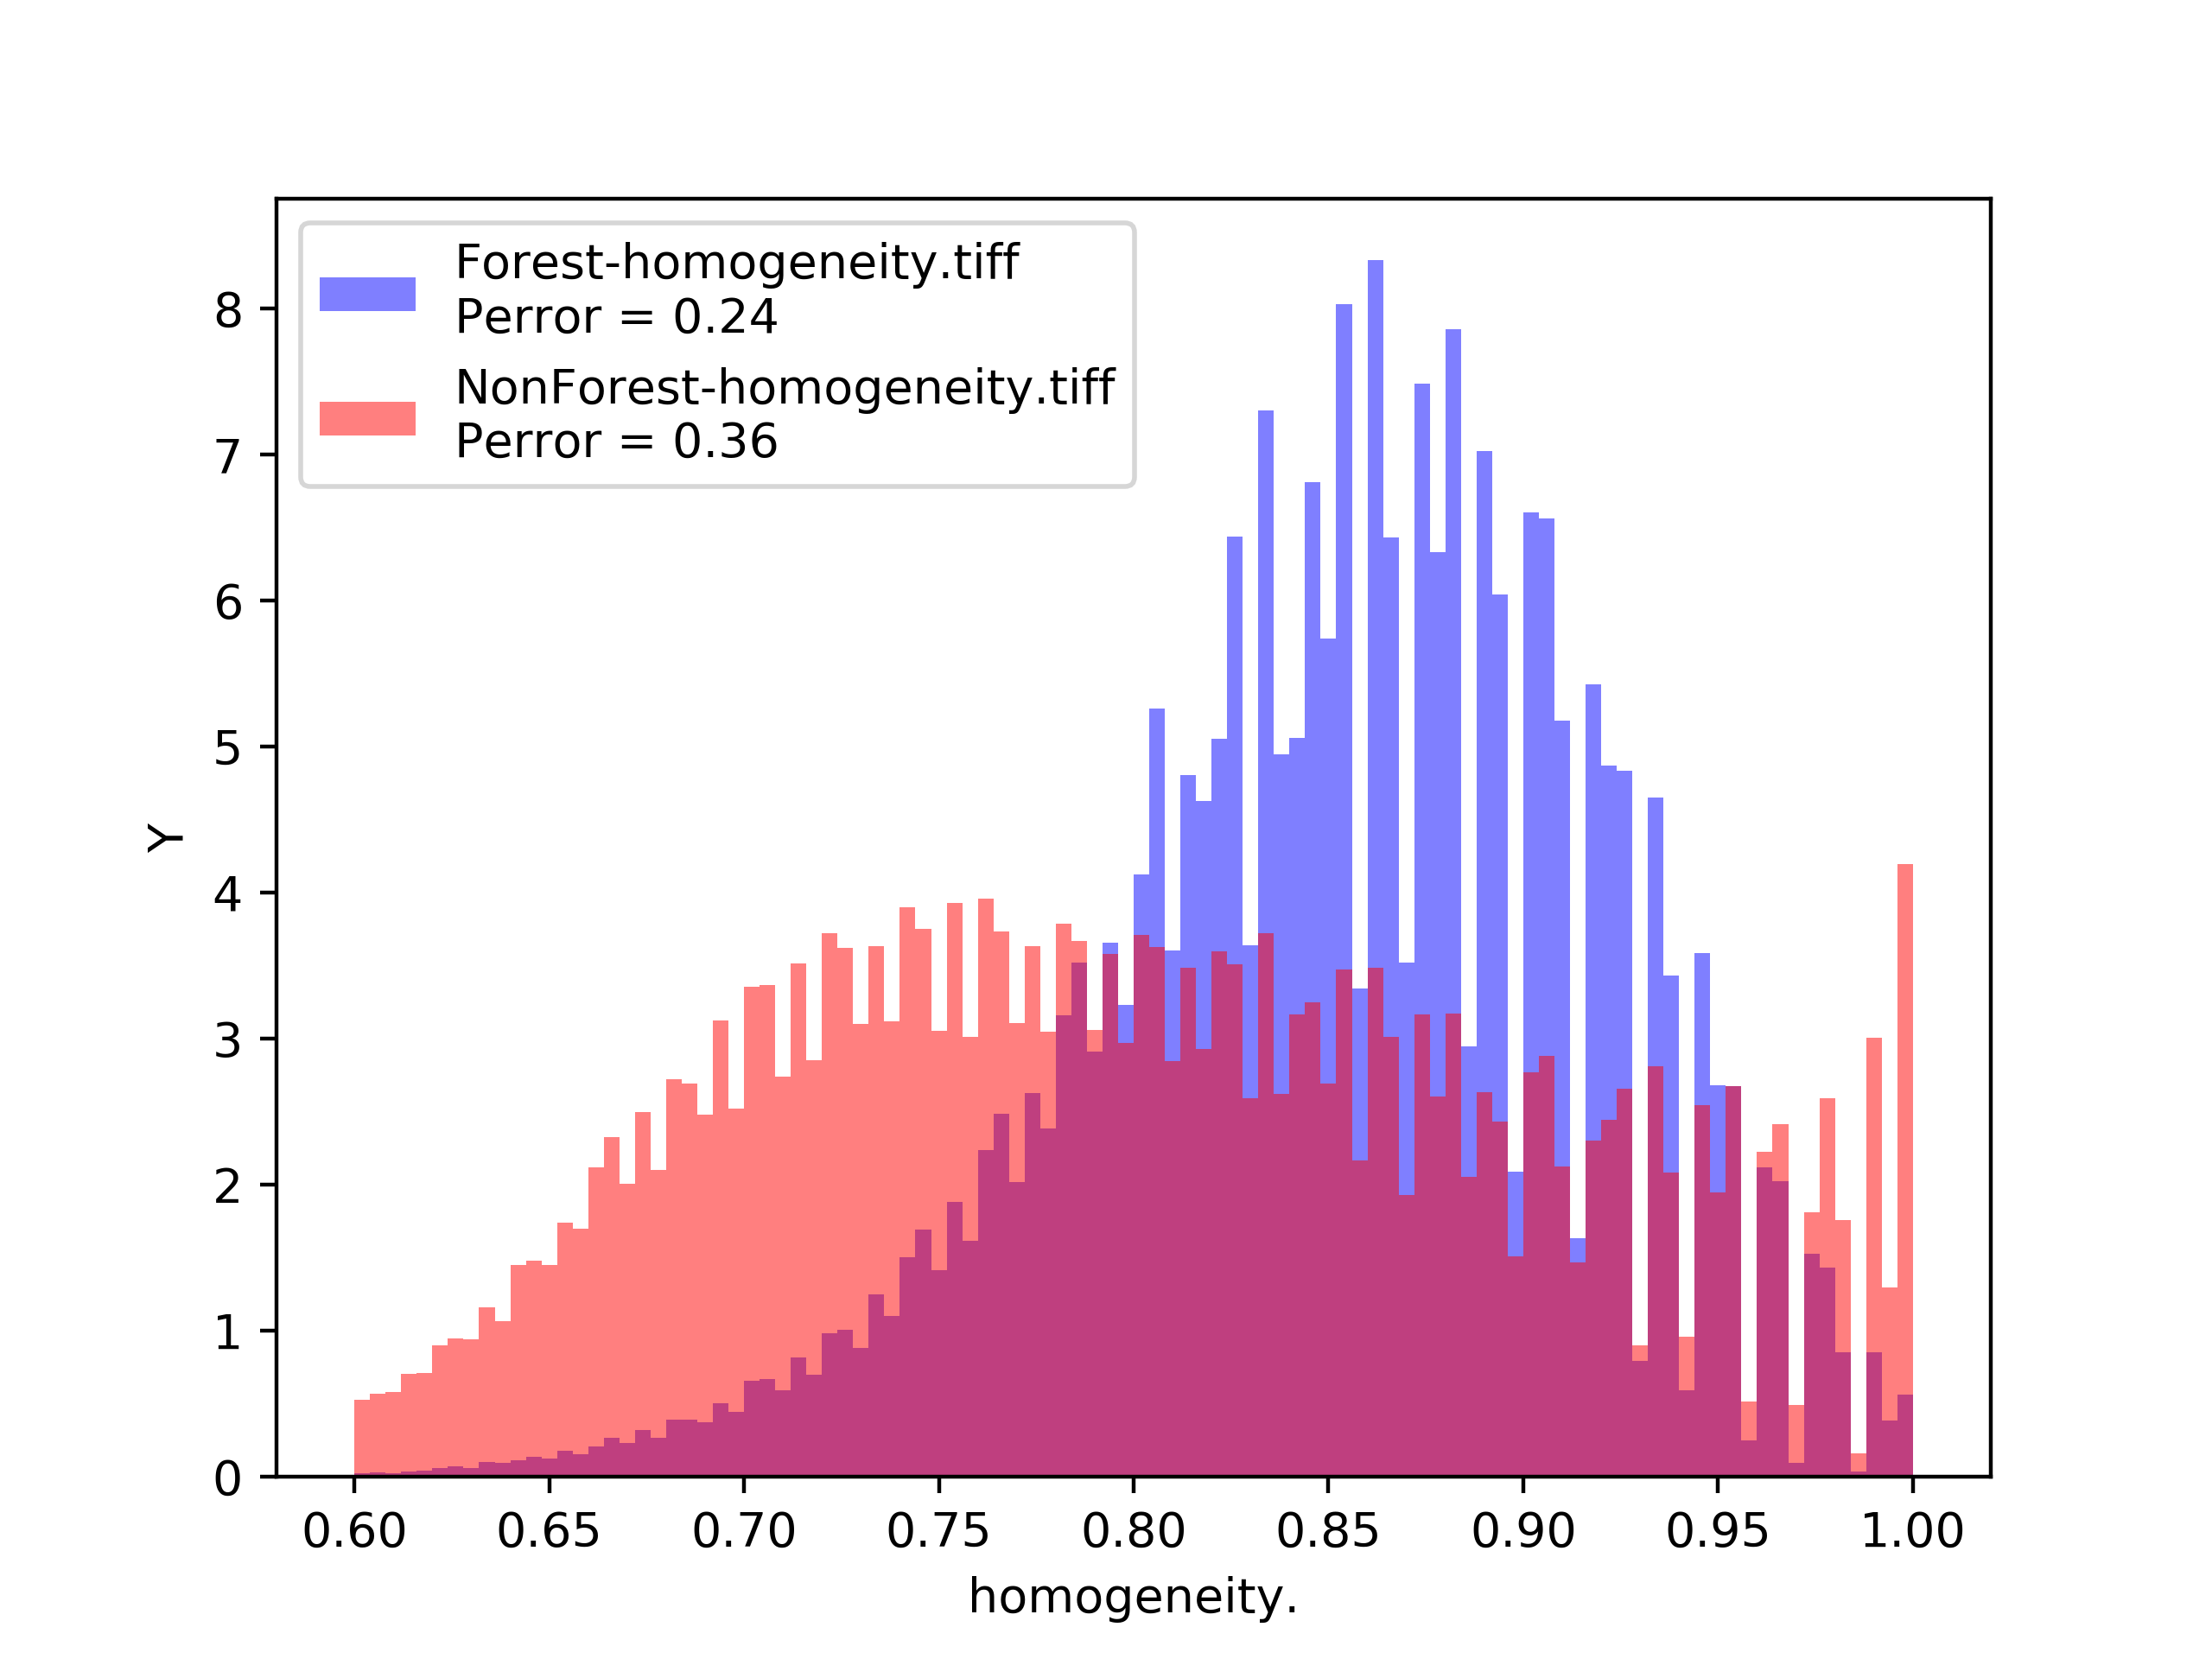
\includegraphics[width=\linewidth]{Chapter4/glcm_textures/homogeneity_hist.png}
     \caption{Probability density Function for Homogeneity.}
  \end{subfigure}
\end{figure}

From the images above it is possible to see clearly that the PDFs of the textures are very different from the PDFs of the coherence, that means that the information contained in the textures is different from the information contained in the coherence, which implies that it is information that can be useful for image segmentation and classification, even if the intersection of PDFs is higher than in the coherence's PDF. 


\section{The Laws Textures results}
\label{sec:laws_textures_results}
As mentioned in the previous chapter, the Laws textures are obtained by applying a series of linear filters to the image. Below there are images of the 9 possible texture results of these filters.

\begin{figure}[H]
  \centering
  \begin{subfigure}[b]{0.4\linewidth}
    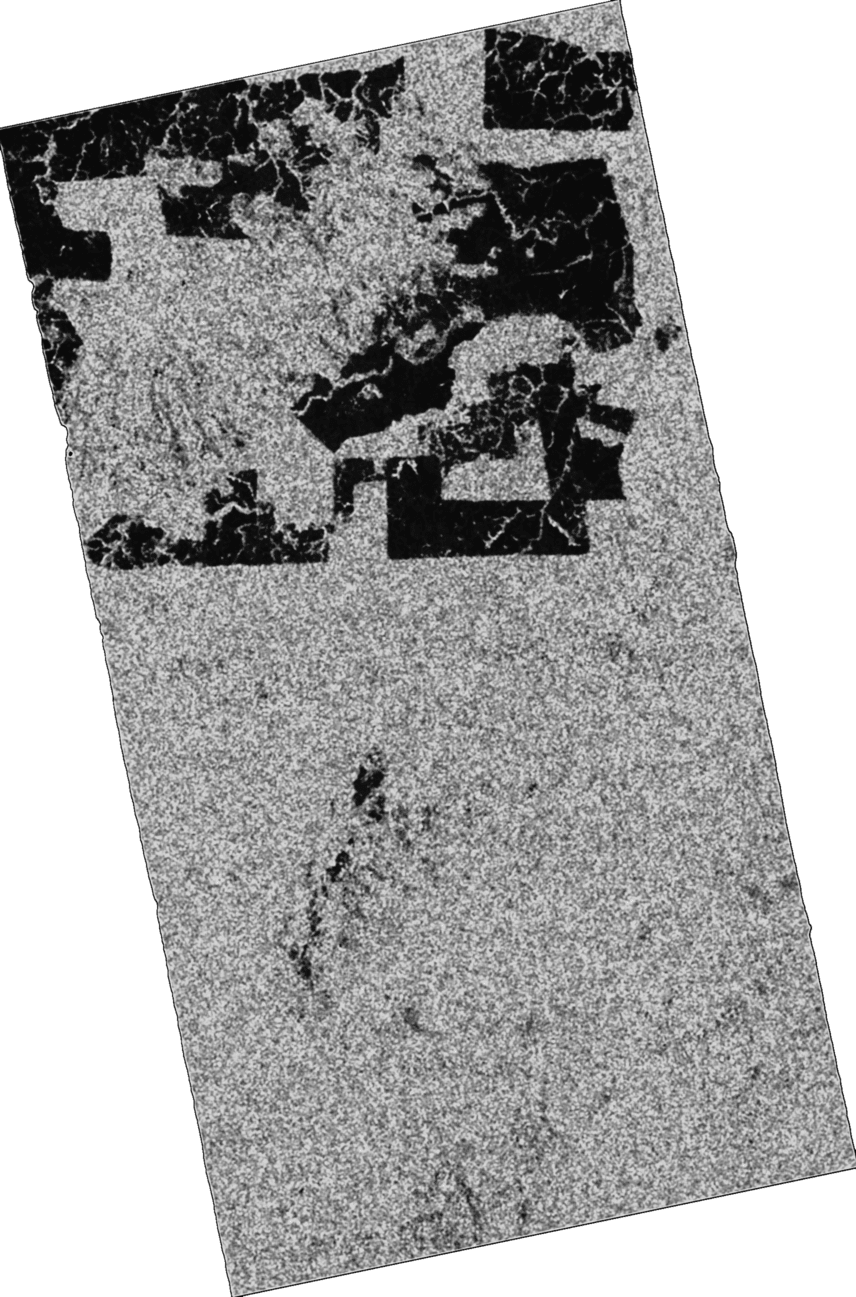
\includegraphics[width=\linewidth]{Chapter4/laws_textures/e5e5_e5e5image.png}
     \caption{Image of e5e5/e5e5 texture.}
  \end{subfigure}
  \centering
  \begin{subfigure}[b]{0.4\linewidth}
    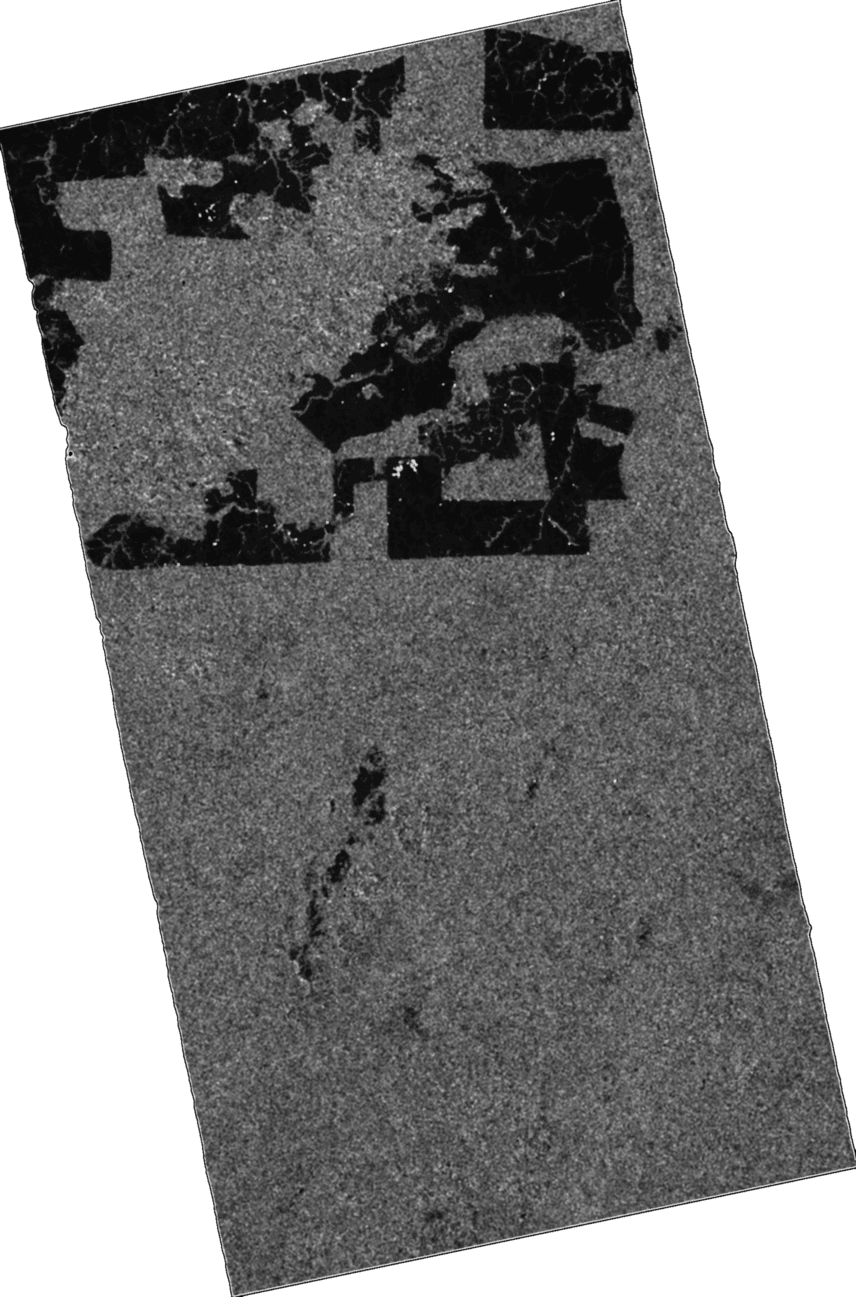
\includegraphics[width=\linewidth]{Chapter4/laws_textures/e5r5_r5e5image.png}
     \caption{Image of e5r5/r5e5 texture.}
  \end{subfigure}
  \centering
  \begin{subfigure}[b]{0.4\linewidth}
    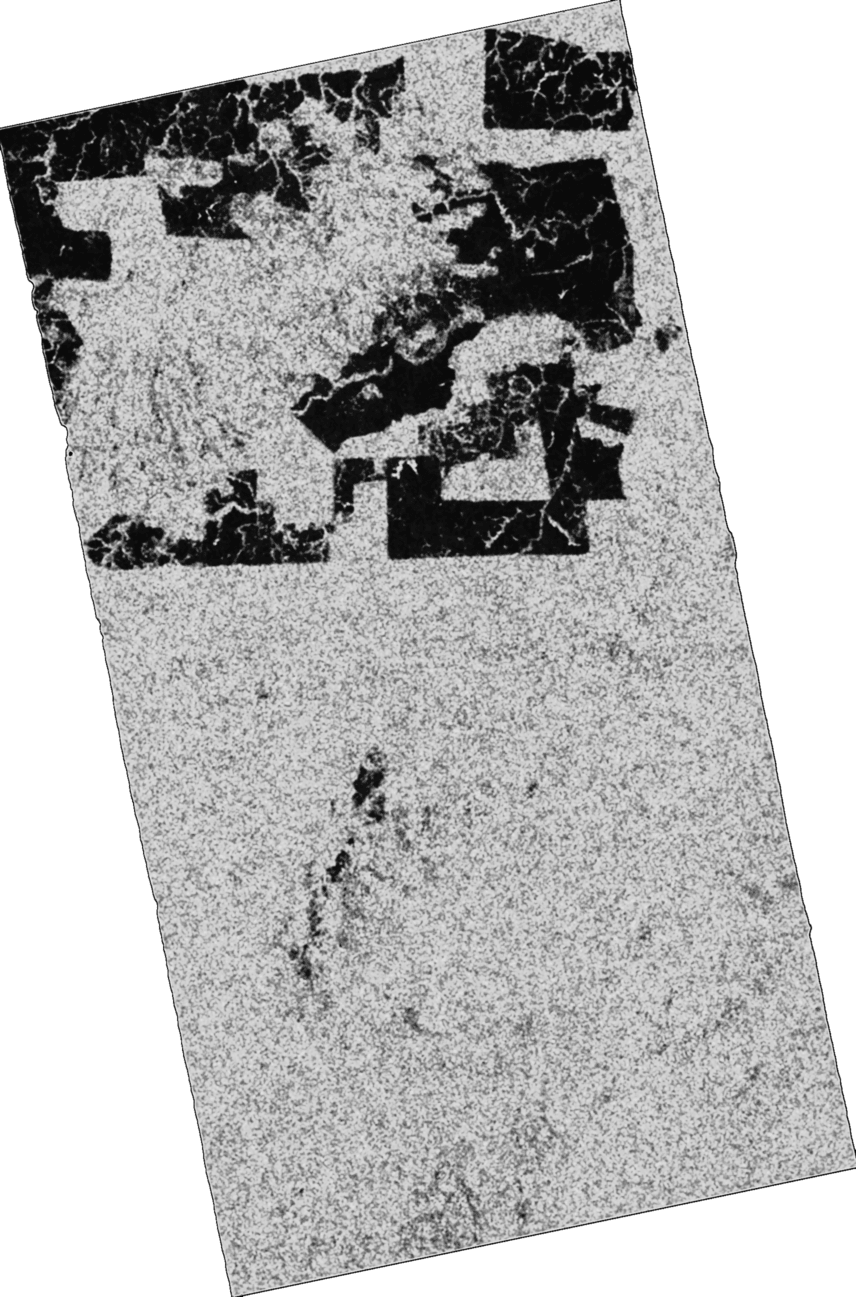
\includegraphics[width=\linewidth]{Chapter4/laws_textures/e5s5_s5e5image.png}
     \caption{Image of e5s5/s5e5 texture.}
  \end{subfigure}
  \centering
  \begin{subfigure}[b]{0.4\linewidth}
    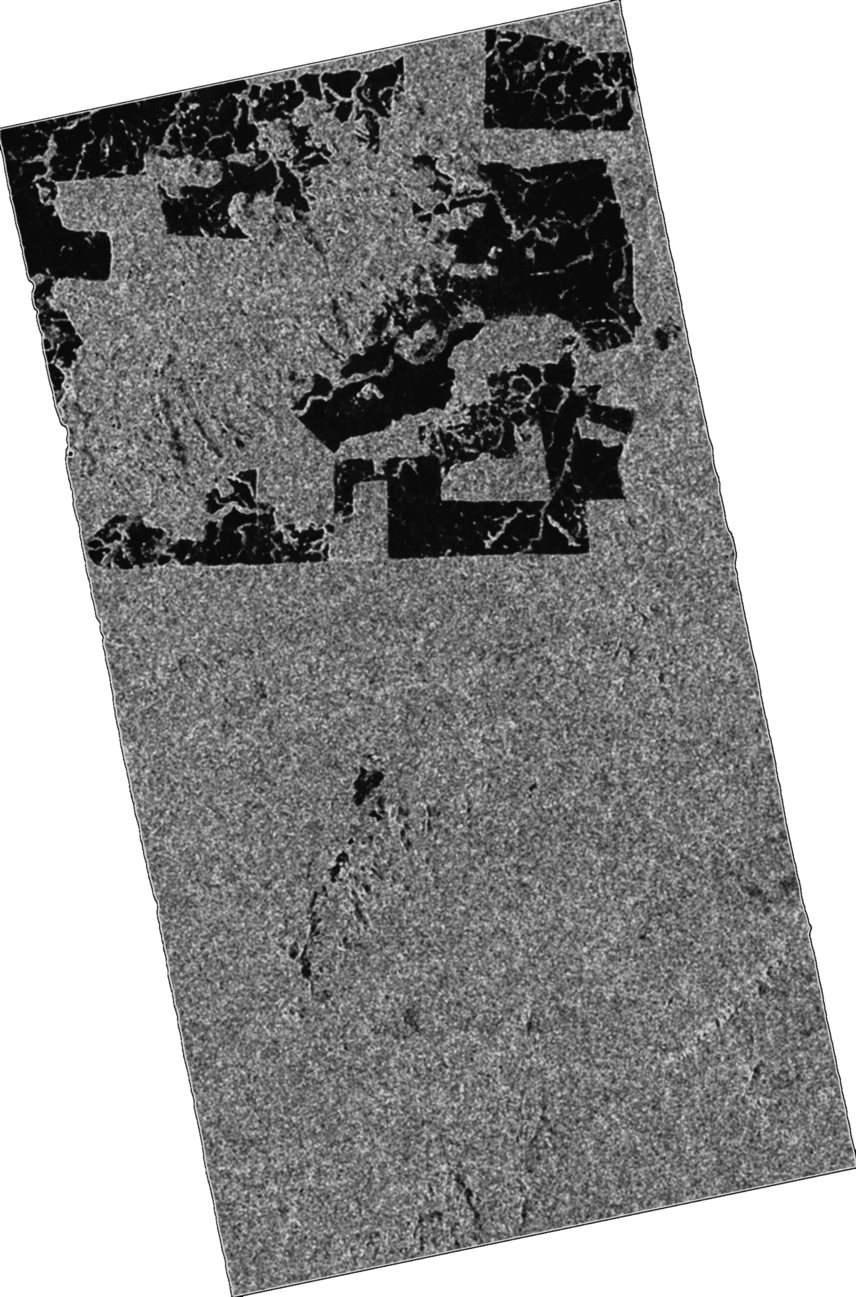
\includegraphics[width=\linewidth]{Chapter4/laws_textures/l5e5_e5l5image.png}
     \caption{Image of l5e5/e5l5 texture.}
  \end{subfigure}
\end{figure}
\newpage
\begin{figure}[H]\ContinuedFloat
  \centering
  \begin{subfigure}[b]{0.4\linewidth}
    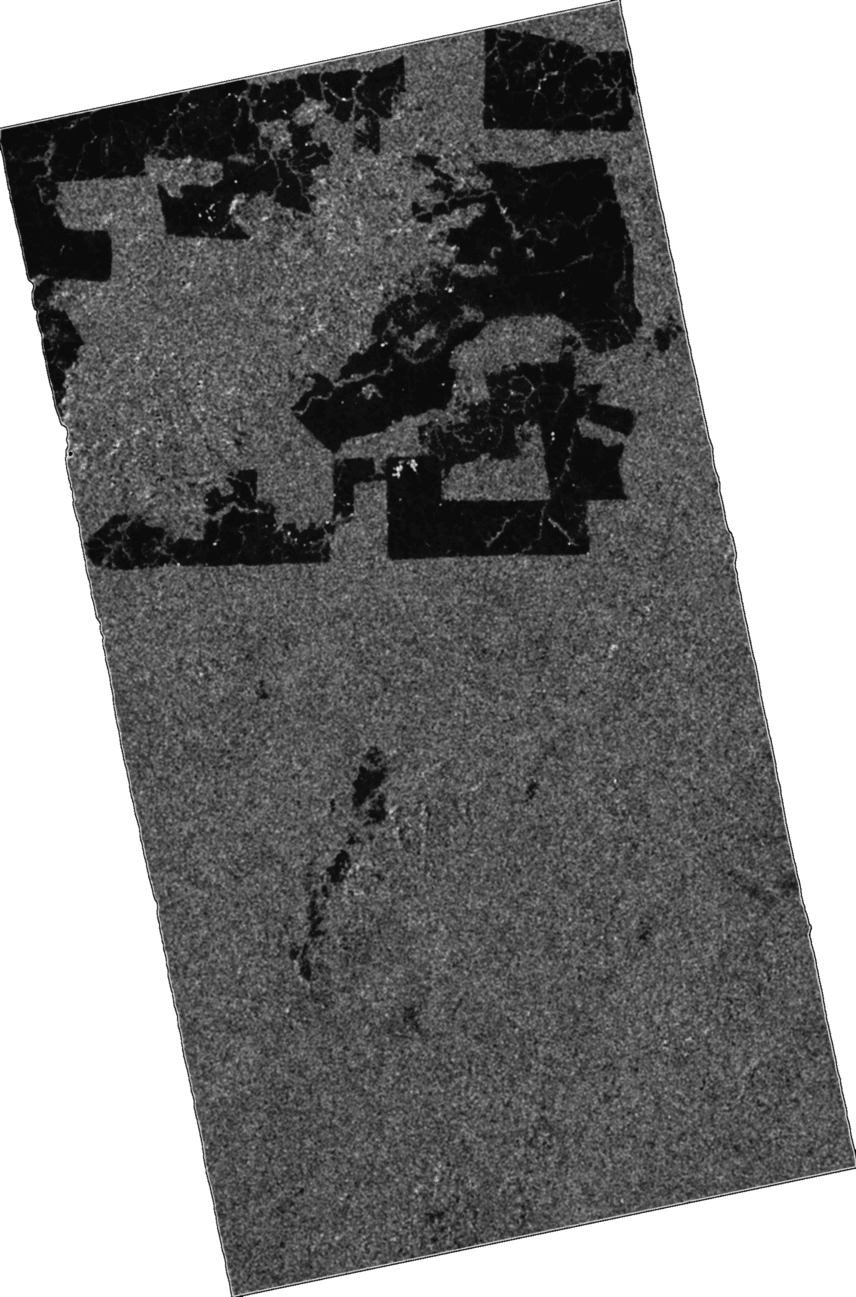
\includegraphics[width=\linewidth]{Chapter4/laws_textures/l5r5_r5l5image.png}
     \caption{Image of l5r5/r5l5 texture.}
  \end{subfigure}
  \centering
  \begin{subfigure}[b]{0.4\linewidth}
    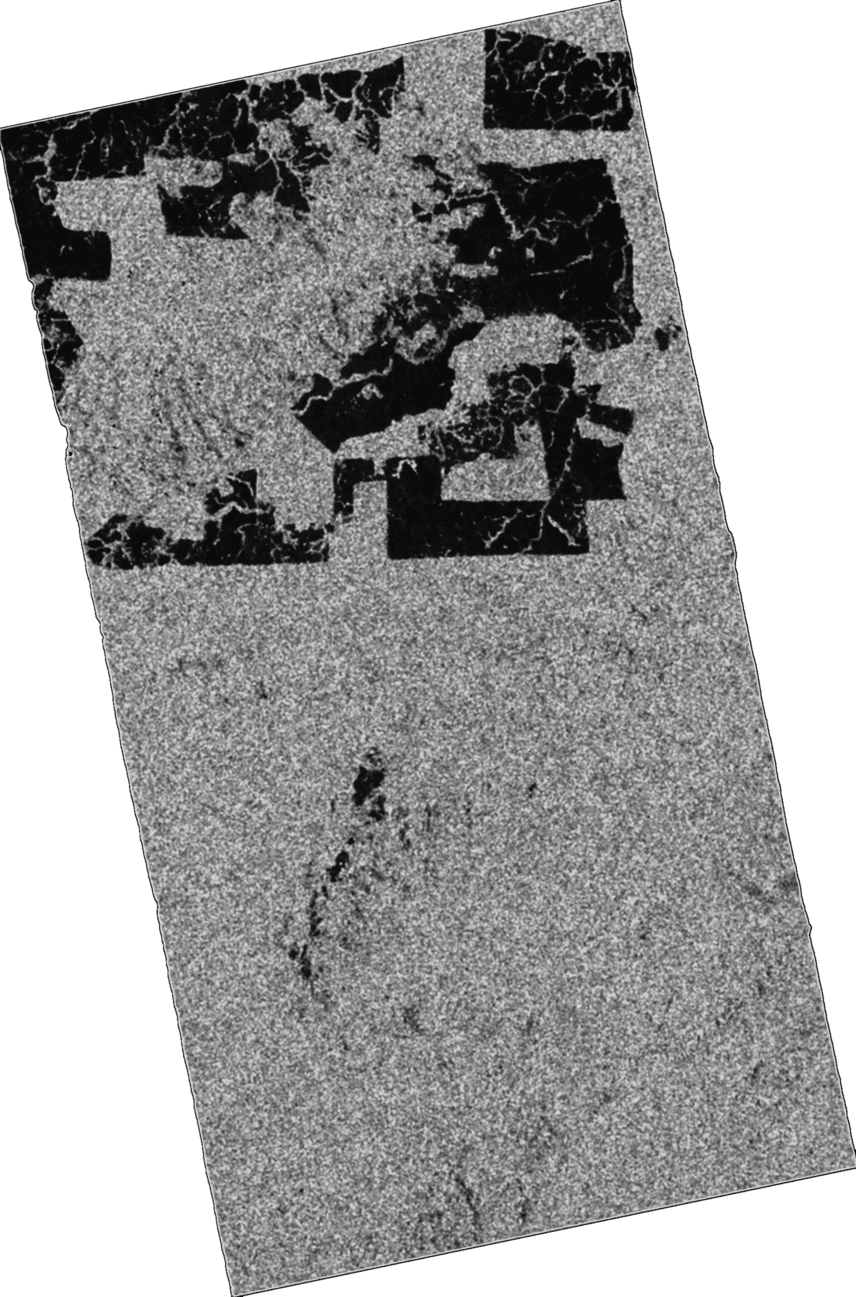
\includegraphics[width=\linewidth]{Chapter4/laws_textures/l5s5_s5l5image.png}
     \caption{Image of l5s5/s5l5 texture.}
  \end{subfigure}
  \centering
  \begin{subfigure}[b]{0.4\linewidth}
    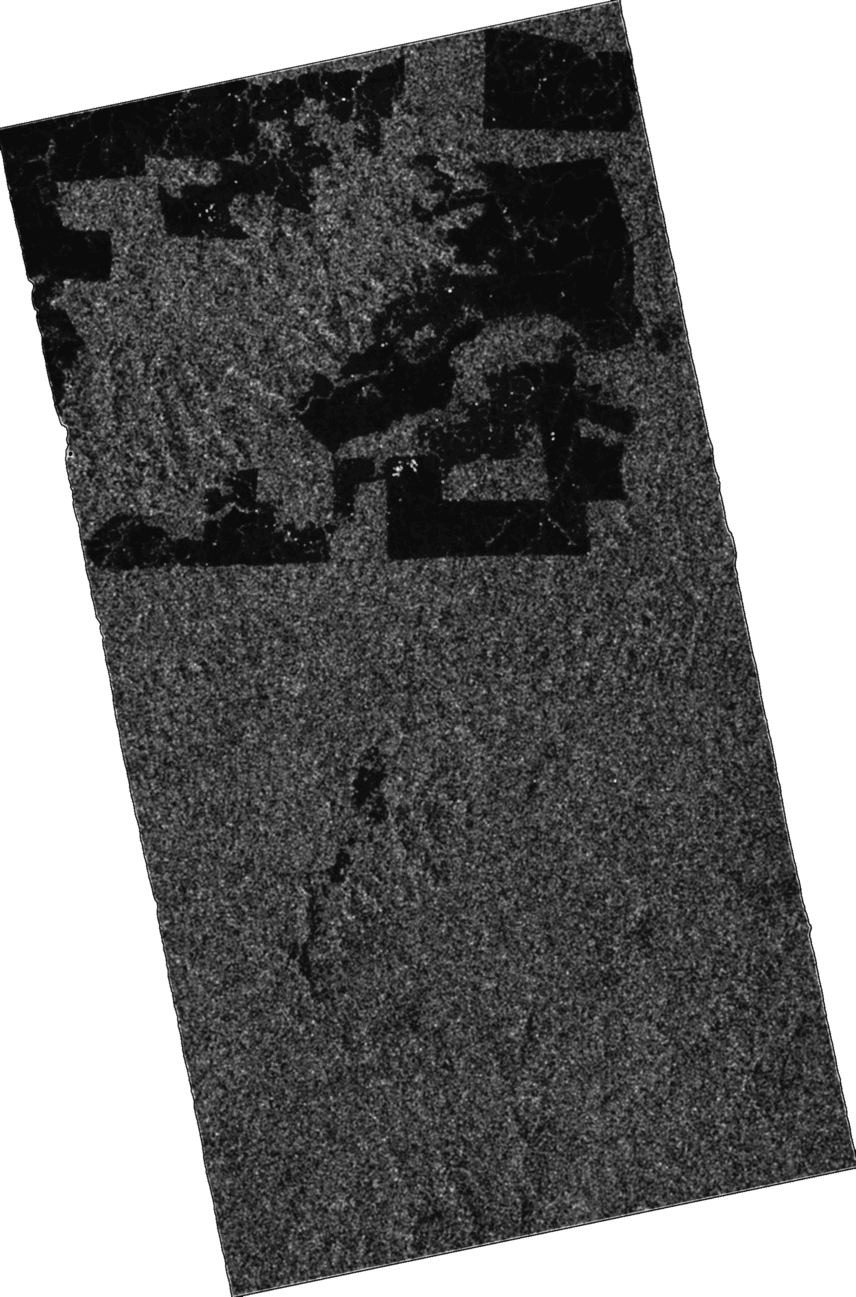
\includegraphics[width=\linewidth]{Chapter4/laws_textures/r5r5_r5r5image.png}
     \caption{Image of r5r5/r5r5 texture.}
  \end{subfigure}
  \centering
  \begin{subfigure}[b]{0.4\linewidth}
    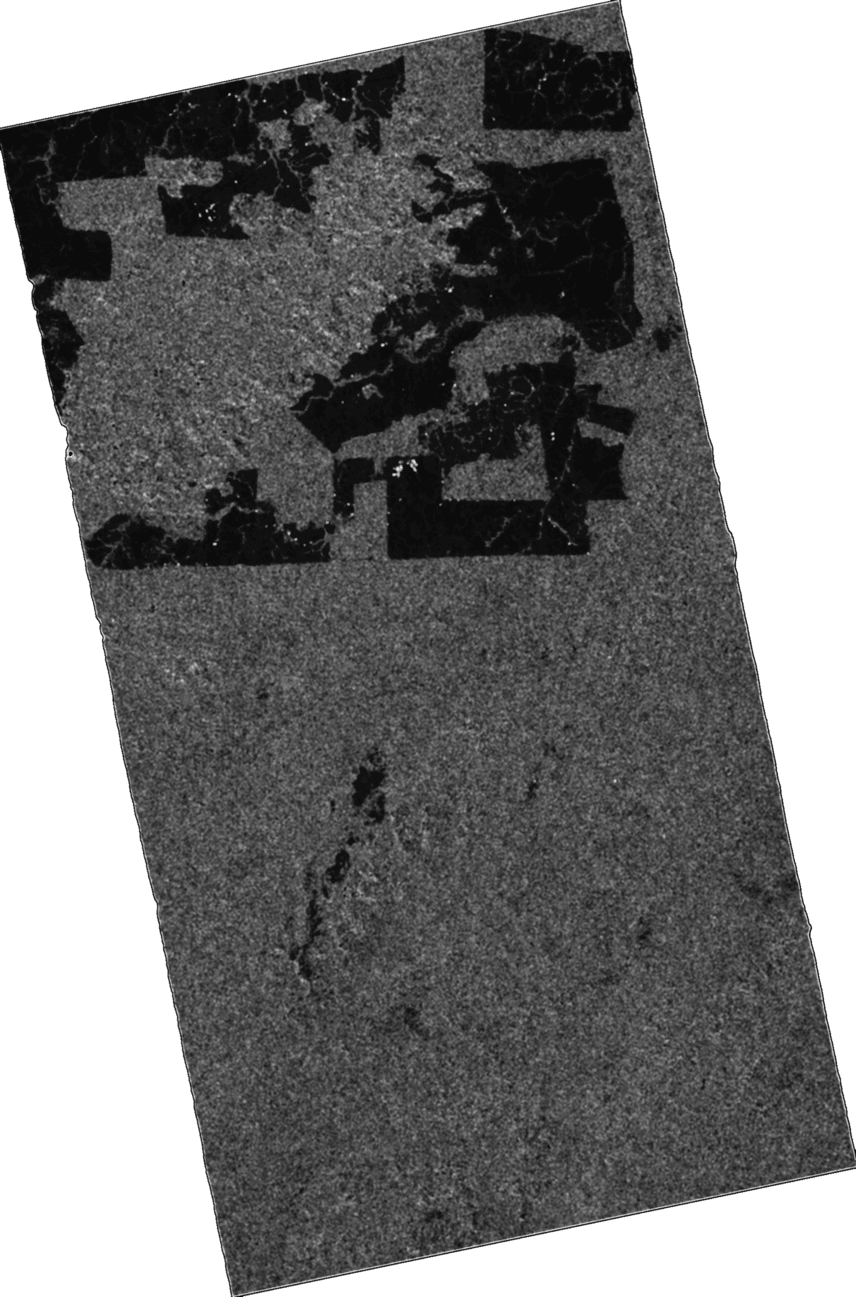
\includegraphics[width=\linewidth]{Chapter4/laws_textures/s5r5_r5s5image.png}
     \caption{Image of s5r5/r5s5 texture.}
  \end{subfigure}
\end{figure}
\newpage
\begin{figure}[H]\ContinuedFloat
  \centering
  \begin{subfigure}[b]{0.4\linewidth}
    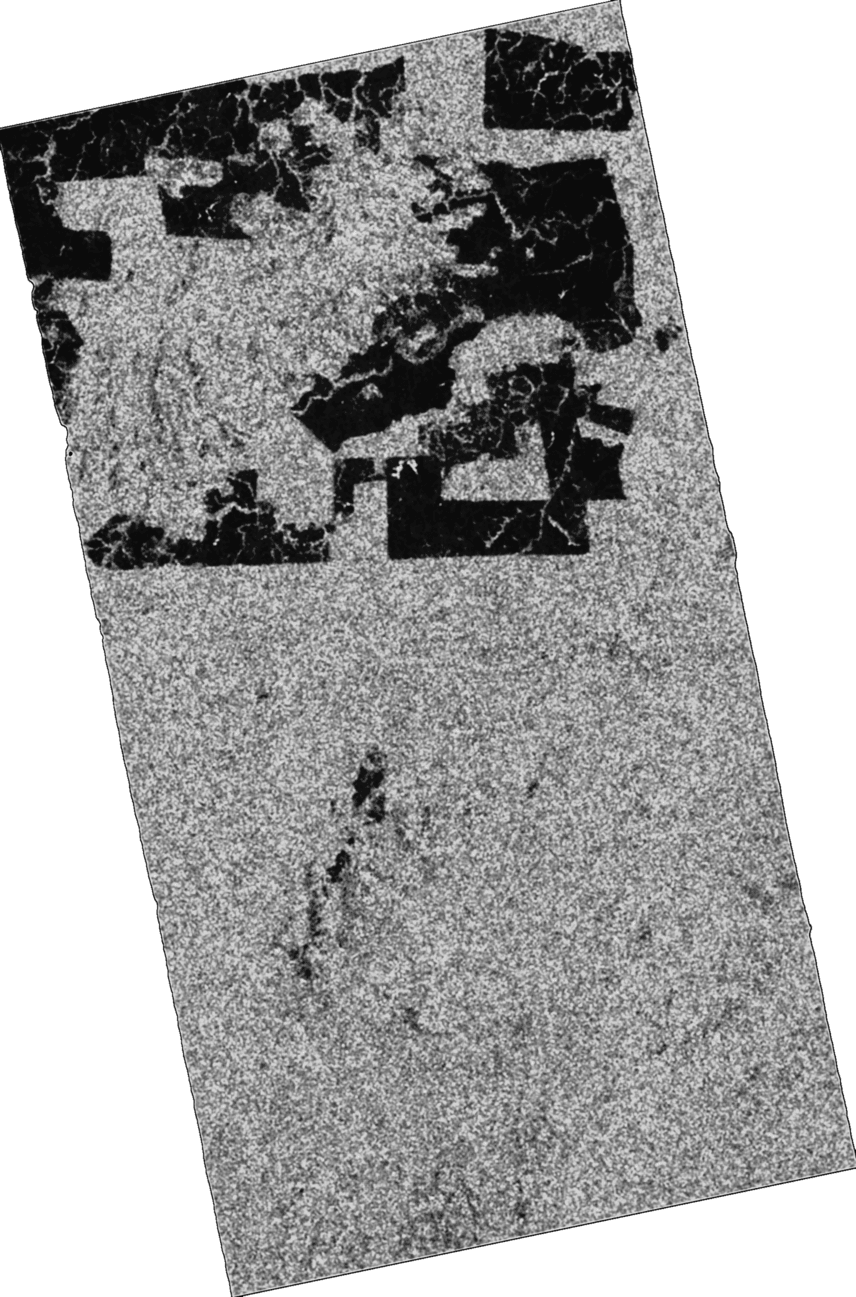
\includegraphics[width=\linewidth]{Chapter4/laws_textures/s5s5_s5s5image.png}
     \caption{Image of s5s5/s5s5 texture.}
  \end{subfigure}
\end{figure}
Again we must look at the PDFs for different classes and see whether they are different from the PDF of the coherence.

\begin{figure}[H]
  \centering
  \begin{subfigure}[b]{0.4\linewidth}
    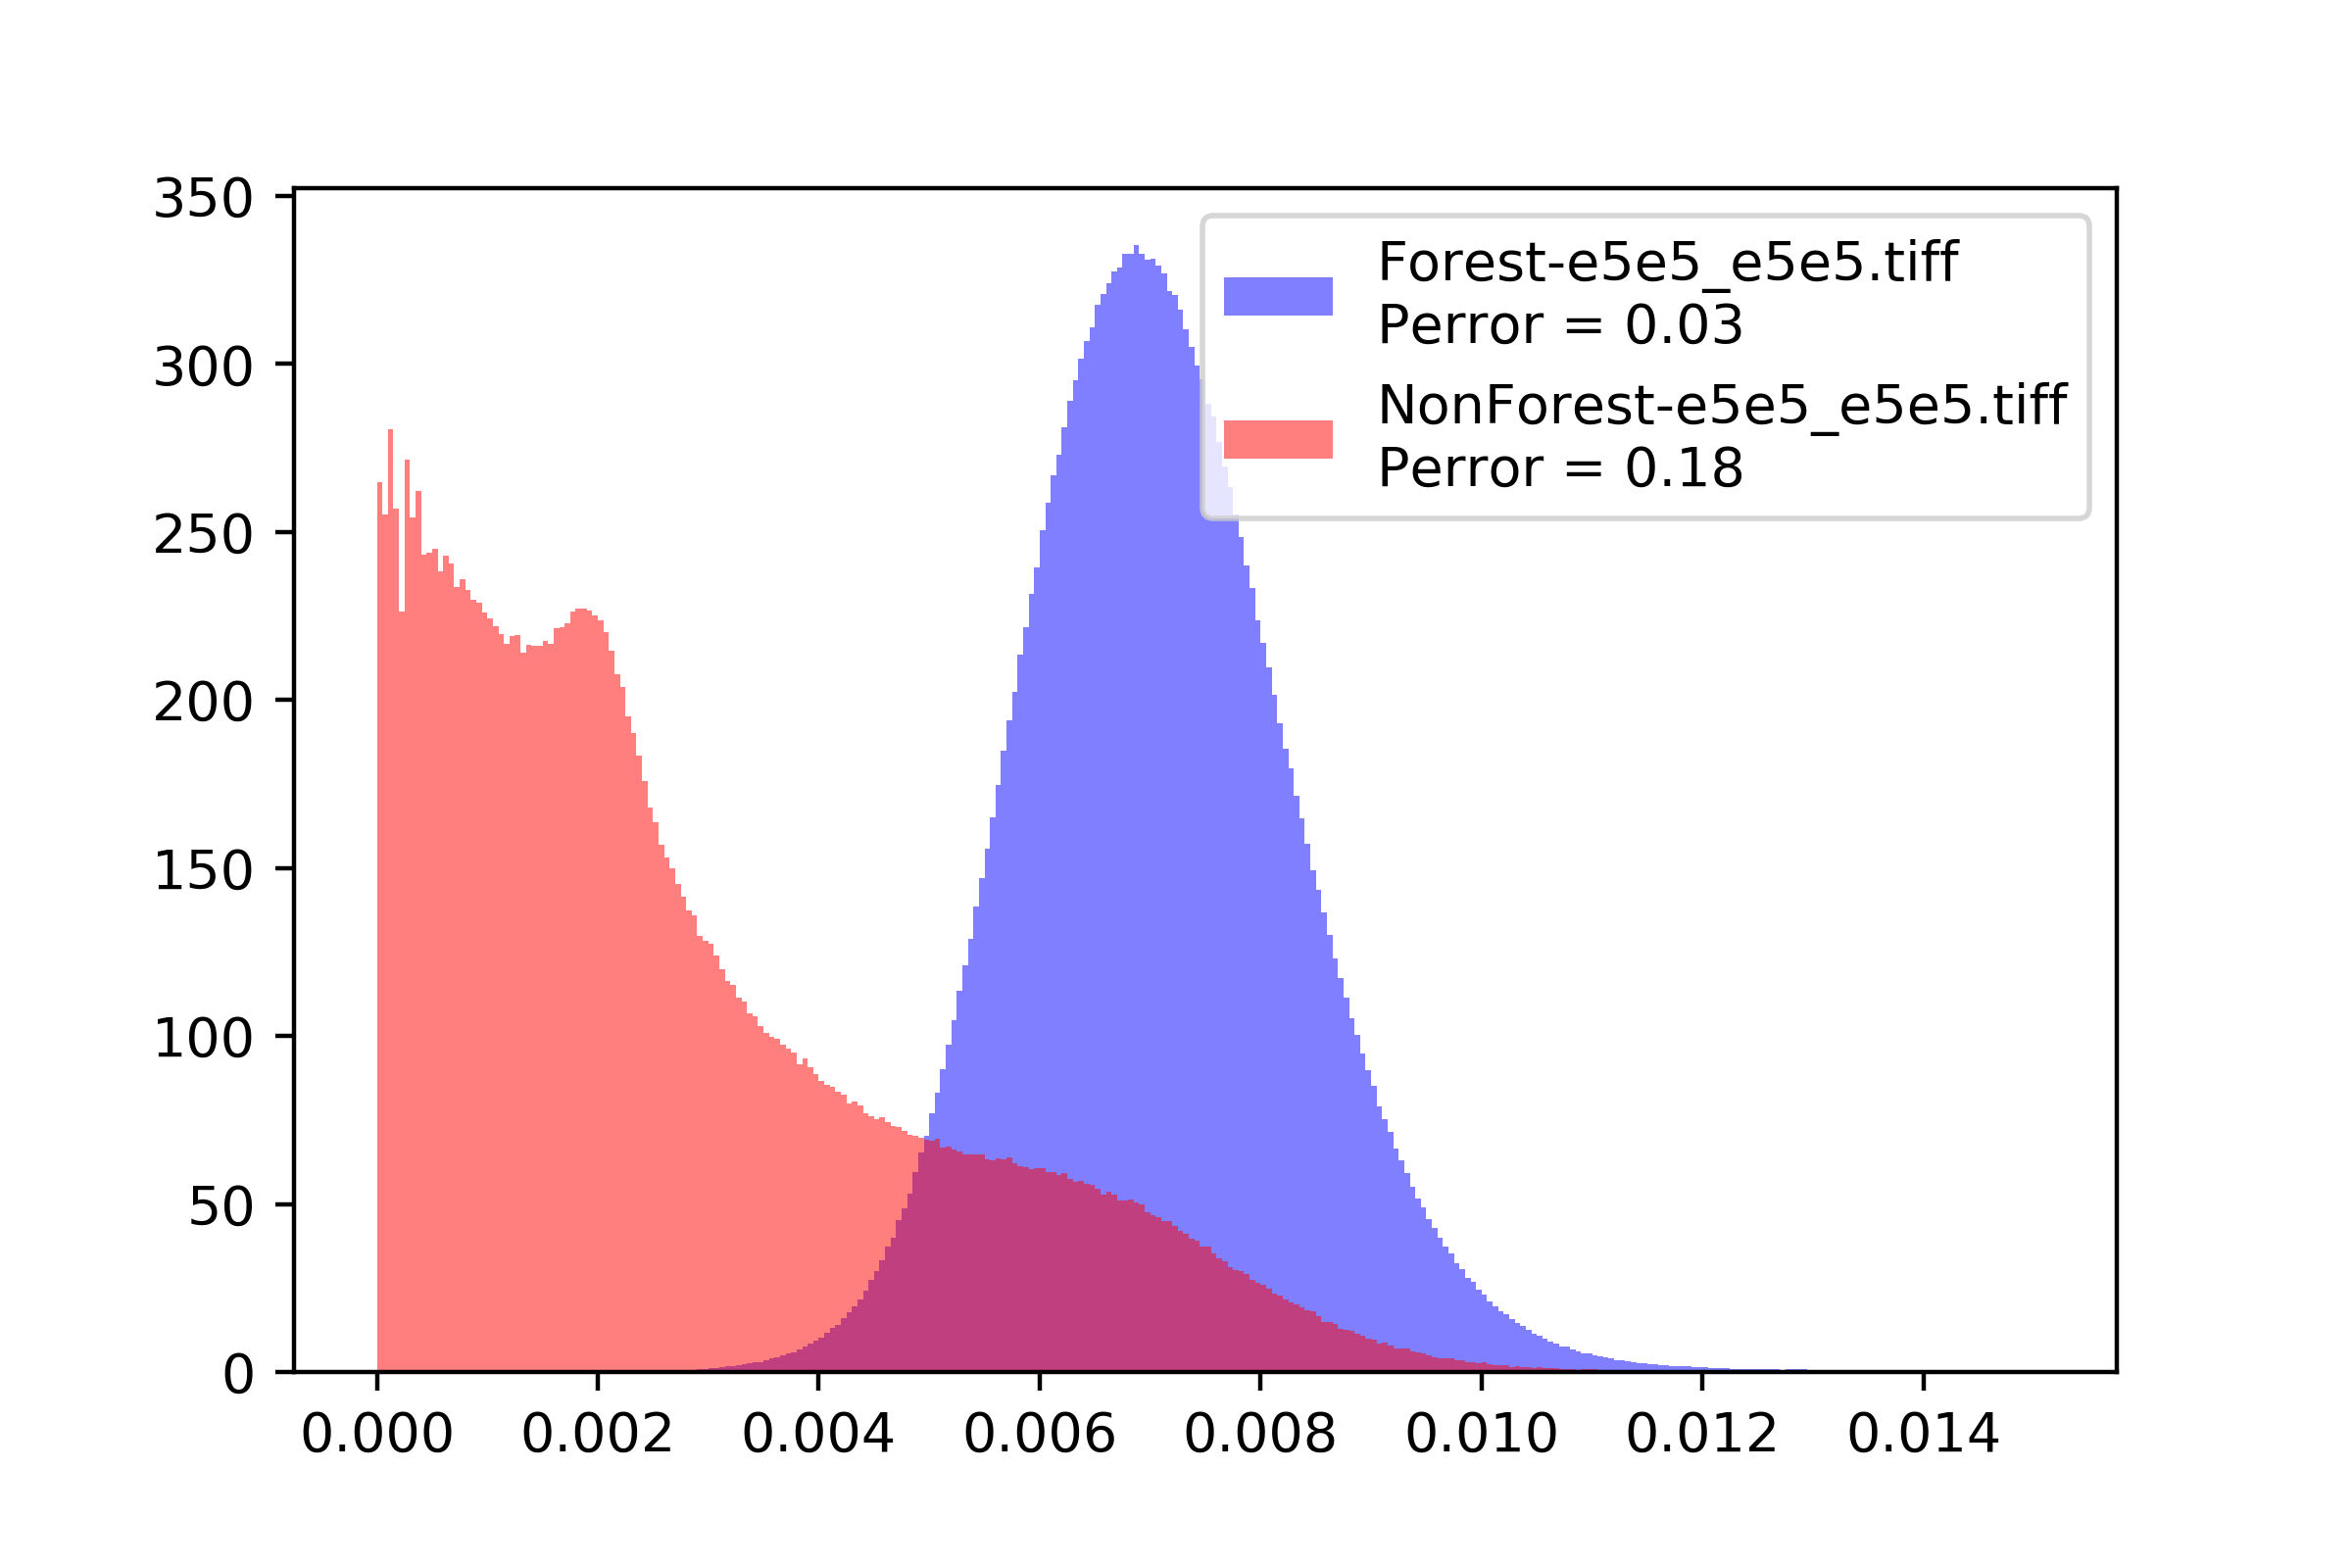
\includegraphics[width=\linewidth]{Chapter4/laws_textures/e5e5_e5e5.png}
     \caption{Probability density Function for e5e5/e5e5.}
  \end{subfigure}
  \centering
  \begin{subfigure}[b]{0.4\linewidth}
    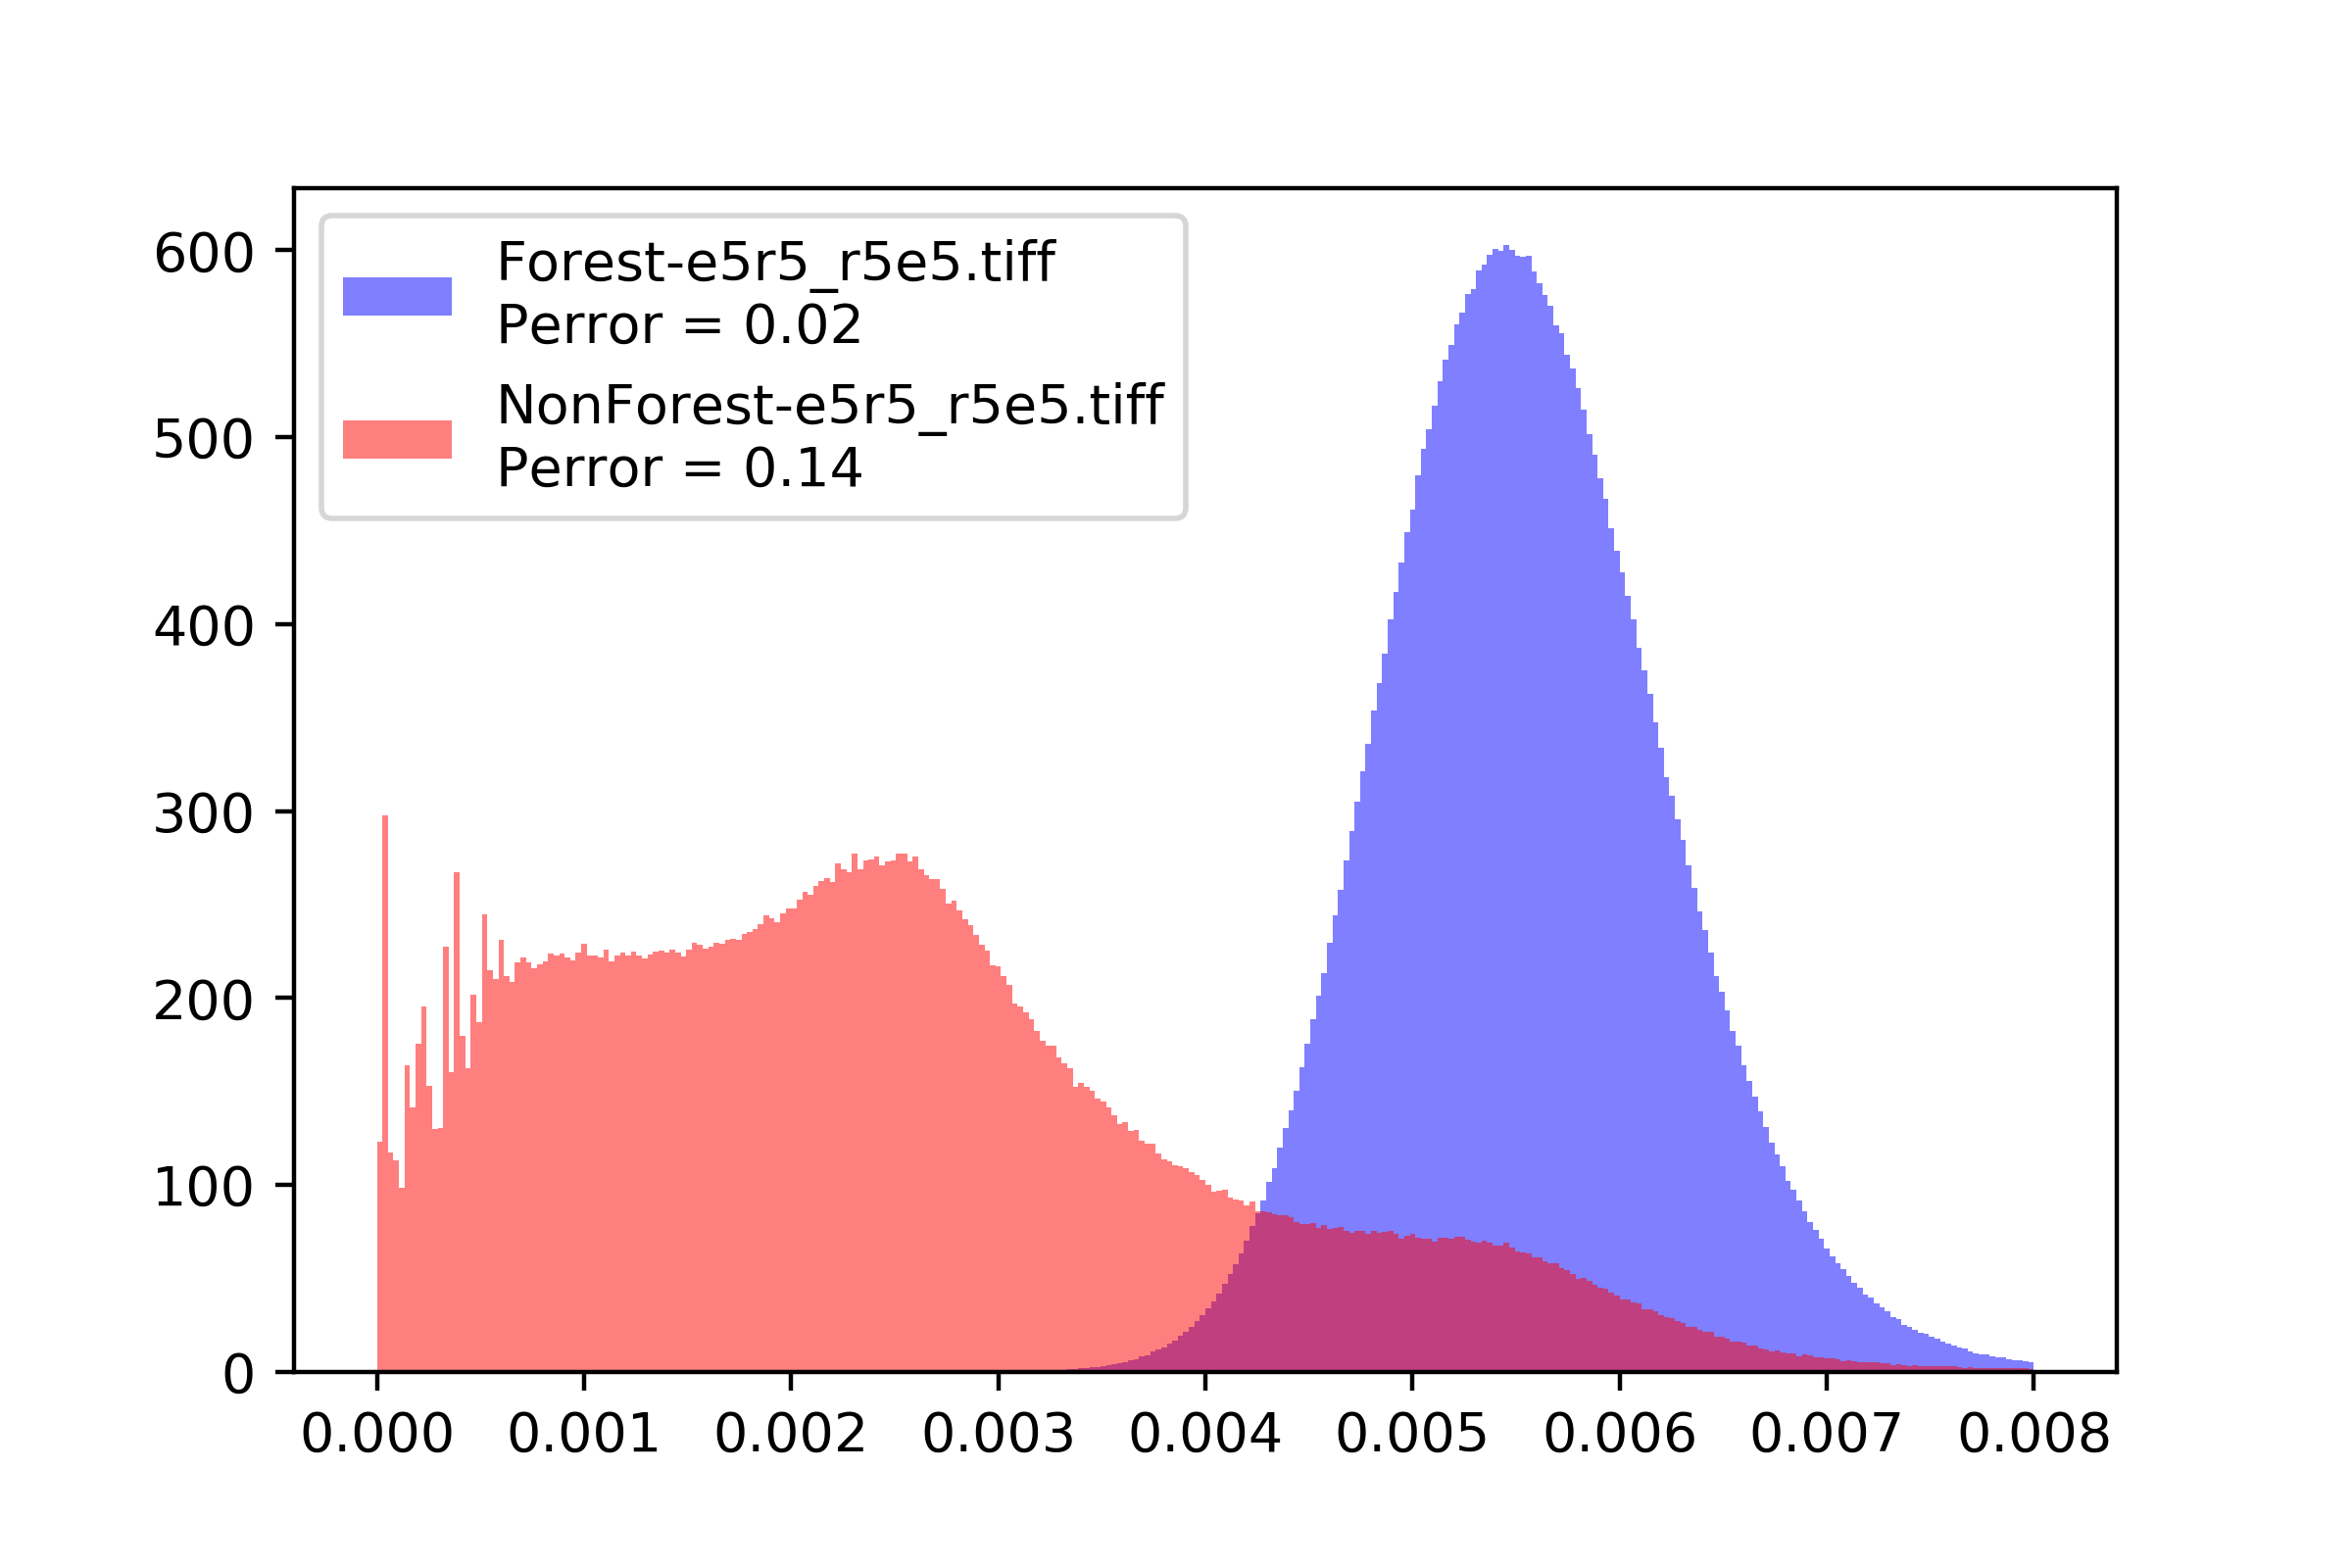
\includegraphics[width=\linewidth]{Chapter4/laws_textures/e5r5_r5e5.png}
     \caption{Probability density Function for e5r5/r5e5.}
  \end{subfigure}
  \centering
  \begin{subfigure}[b]{0.4\linewidth}
    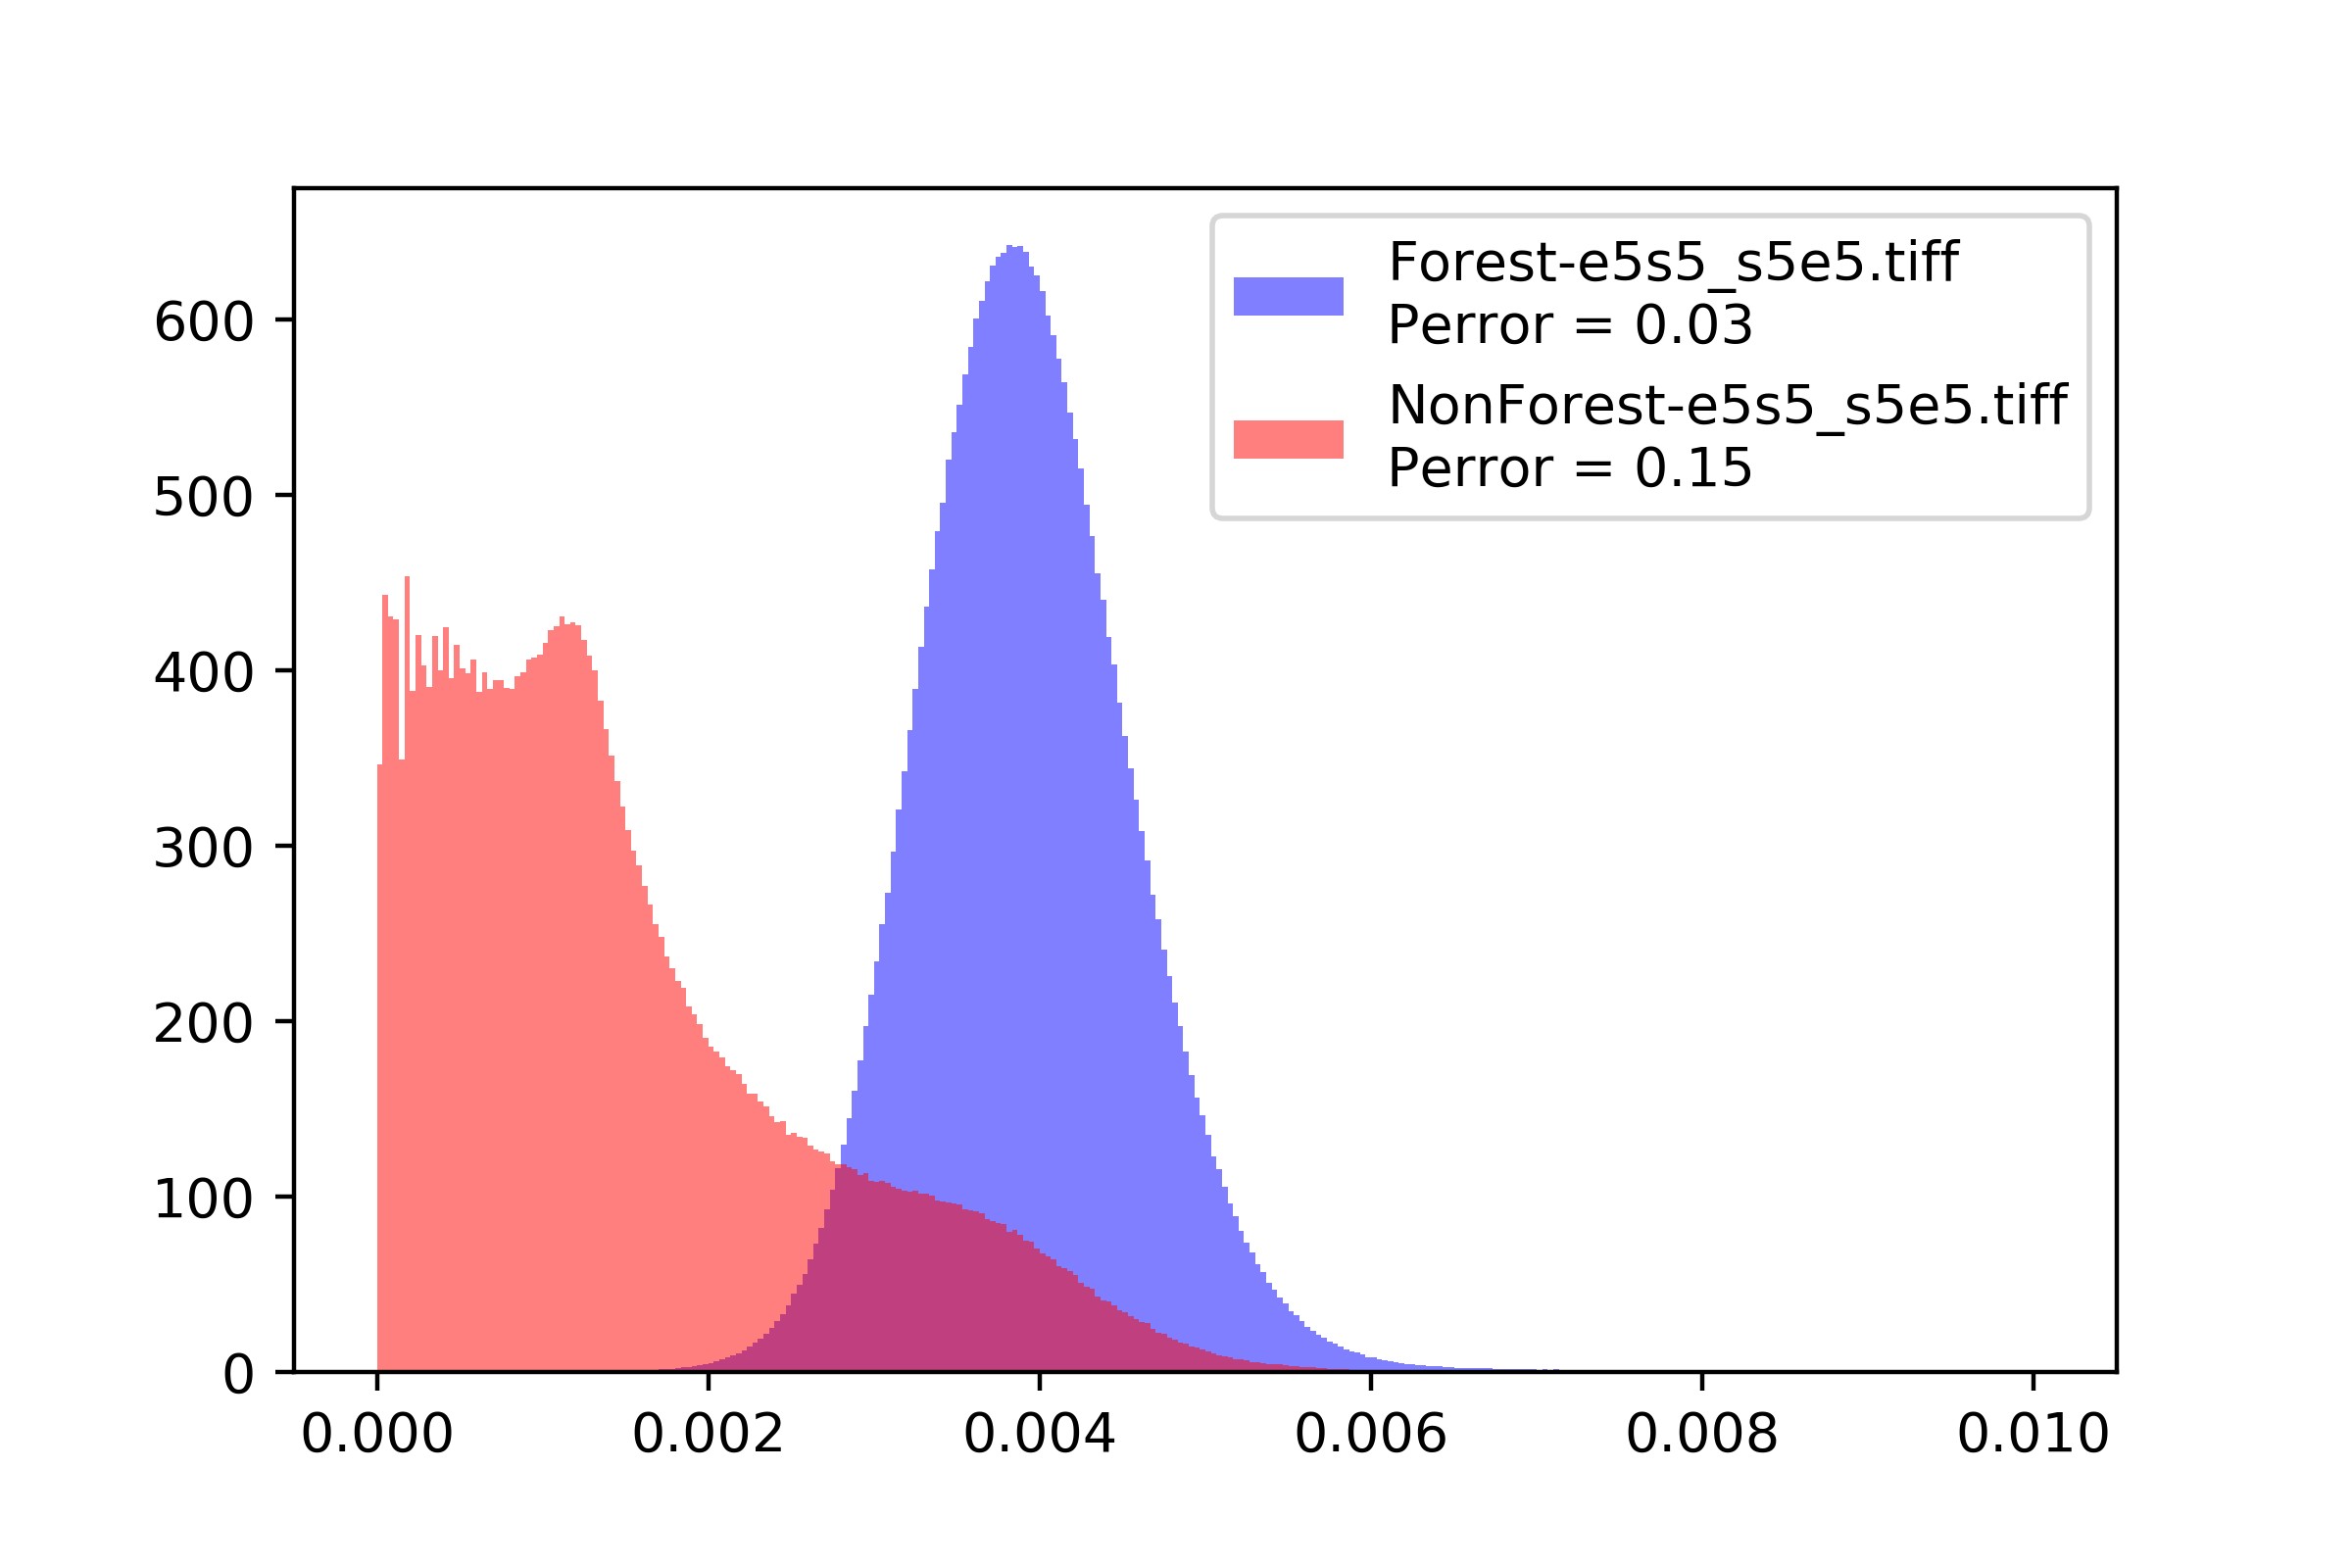
\includegraphics[width=\linewidth]{Chapter4/laws_textures/e5s5_s5e5.png}
     \caption{Probability density Function for e5s5/s5e5.}
  \end{subfigure}
  \centering
  \begin{subfigure}[b]{0.4\linewidth}
    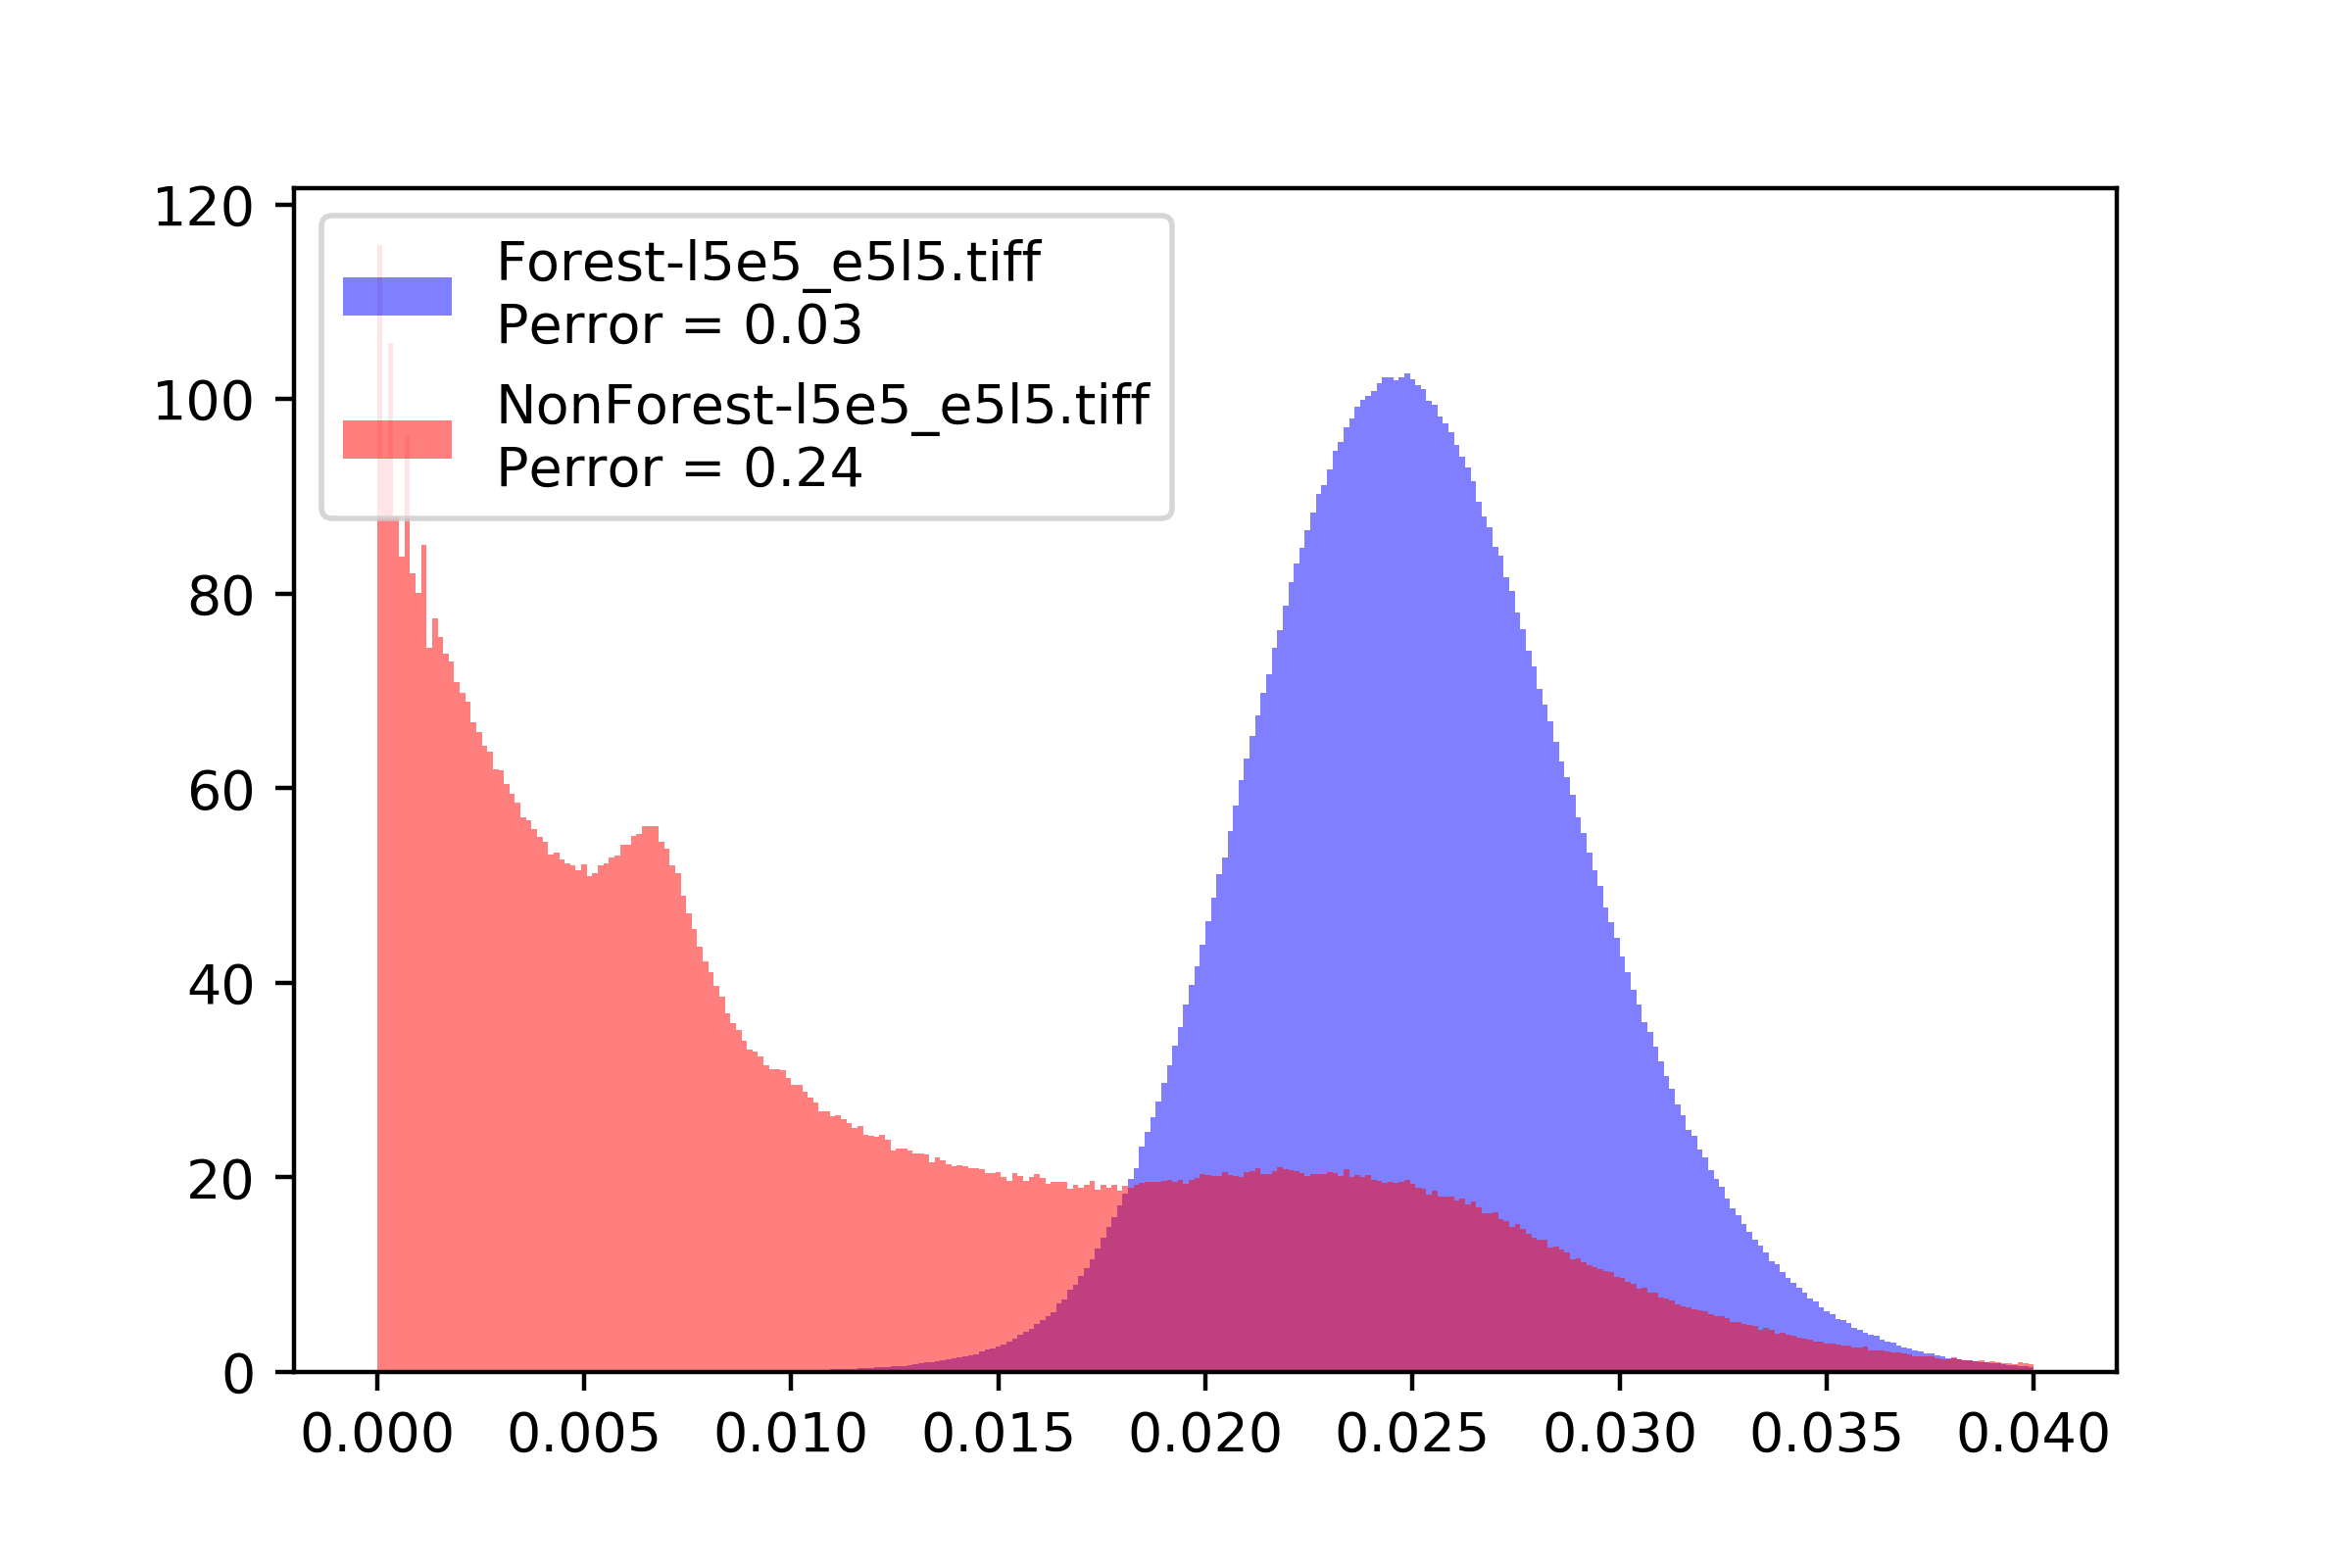
\includegraphics[width=\linewidth]{Chapter4/laws_textures/l5e5_e5l5.png}
     \caption{Probability density Function for l5e5/e5l5.}
  \end{subfigure}
  \centering
  \begin{subfigure}[b]{0.4\linewidth}
    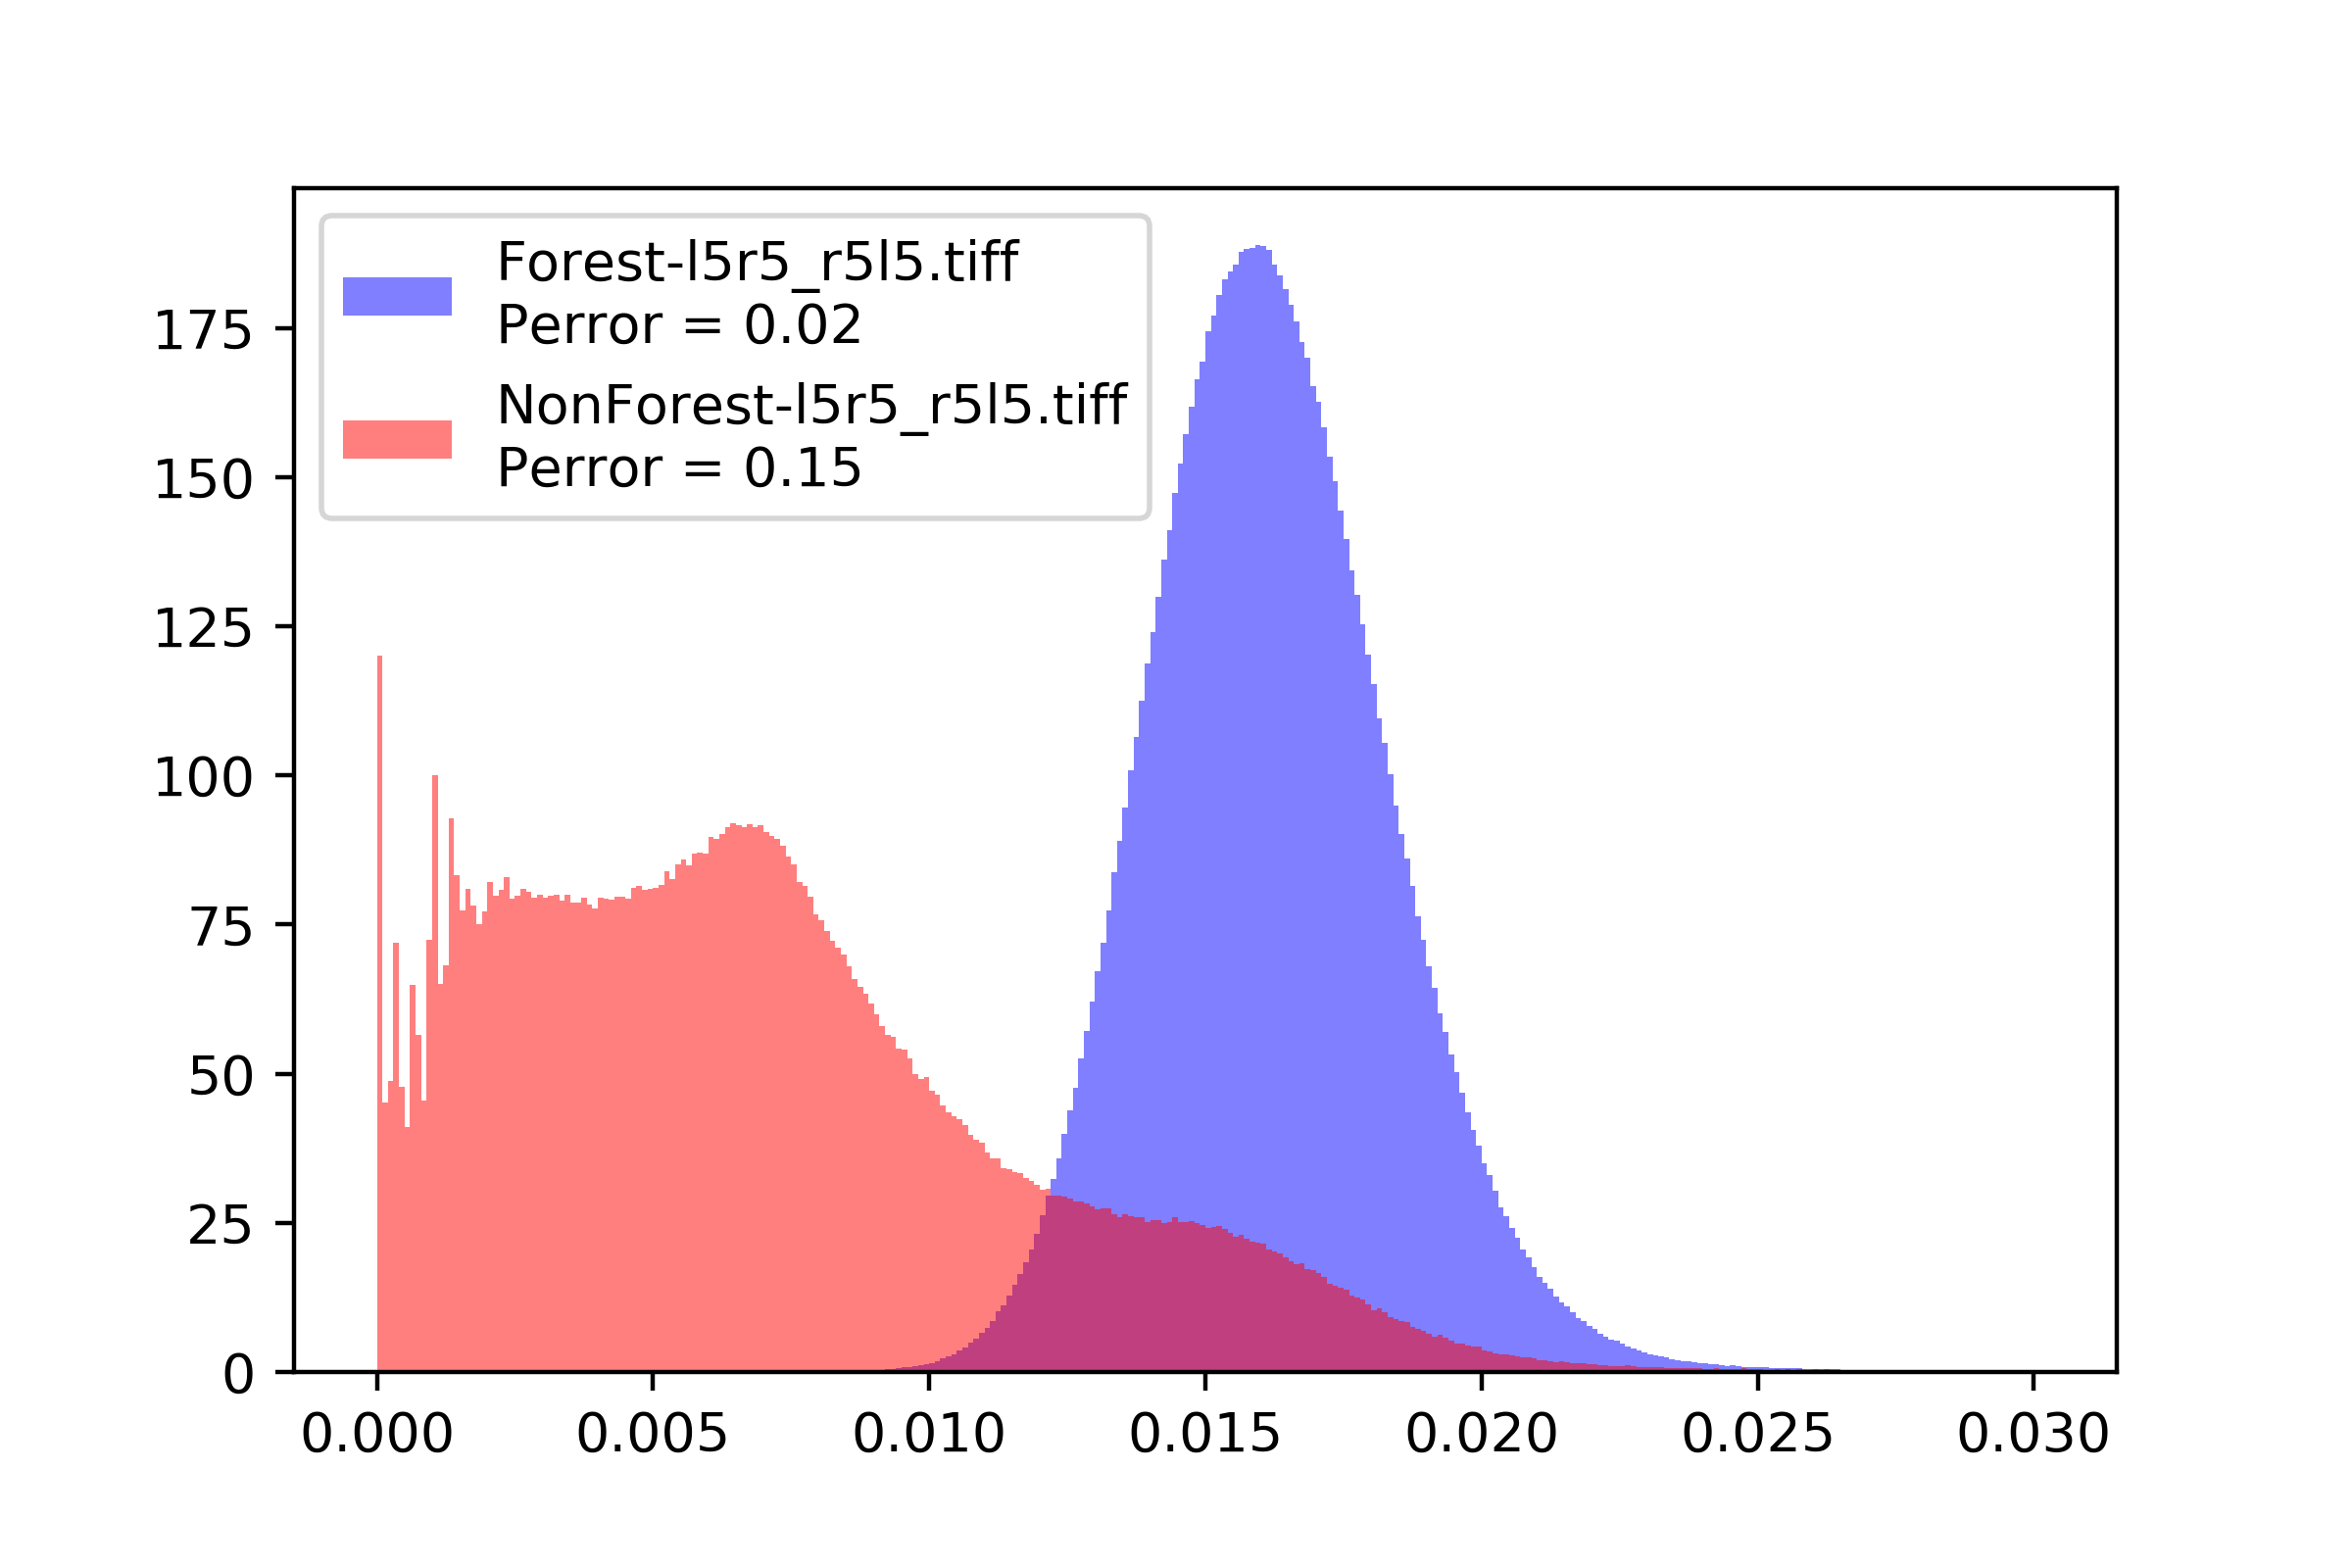
\includegraphics[width=\linewidth]{Chapter4/laws_textures/l5r5_r5l5.png}
     \caption{Probability density Function for l5r5/r5l5.}
  \end{subfigure}
  \centering
  \begin{subfigure}[b]{0.4\linewidth}
    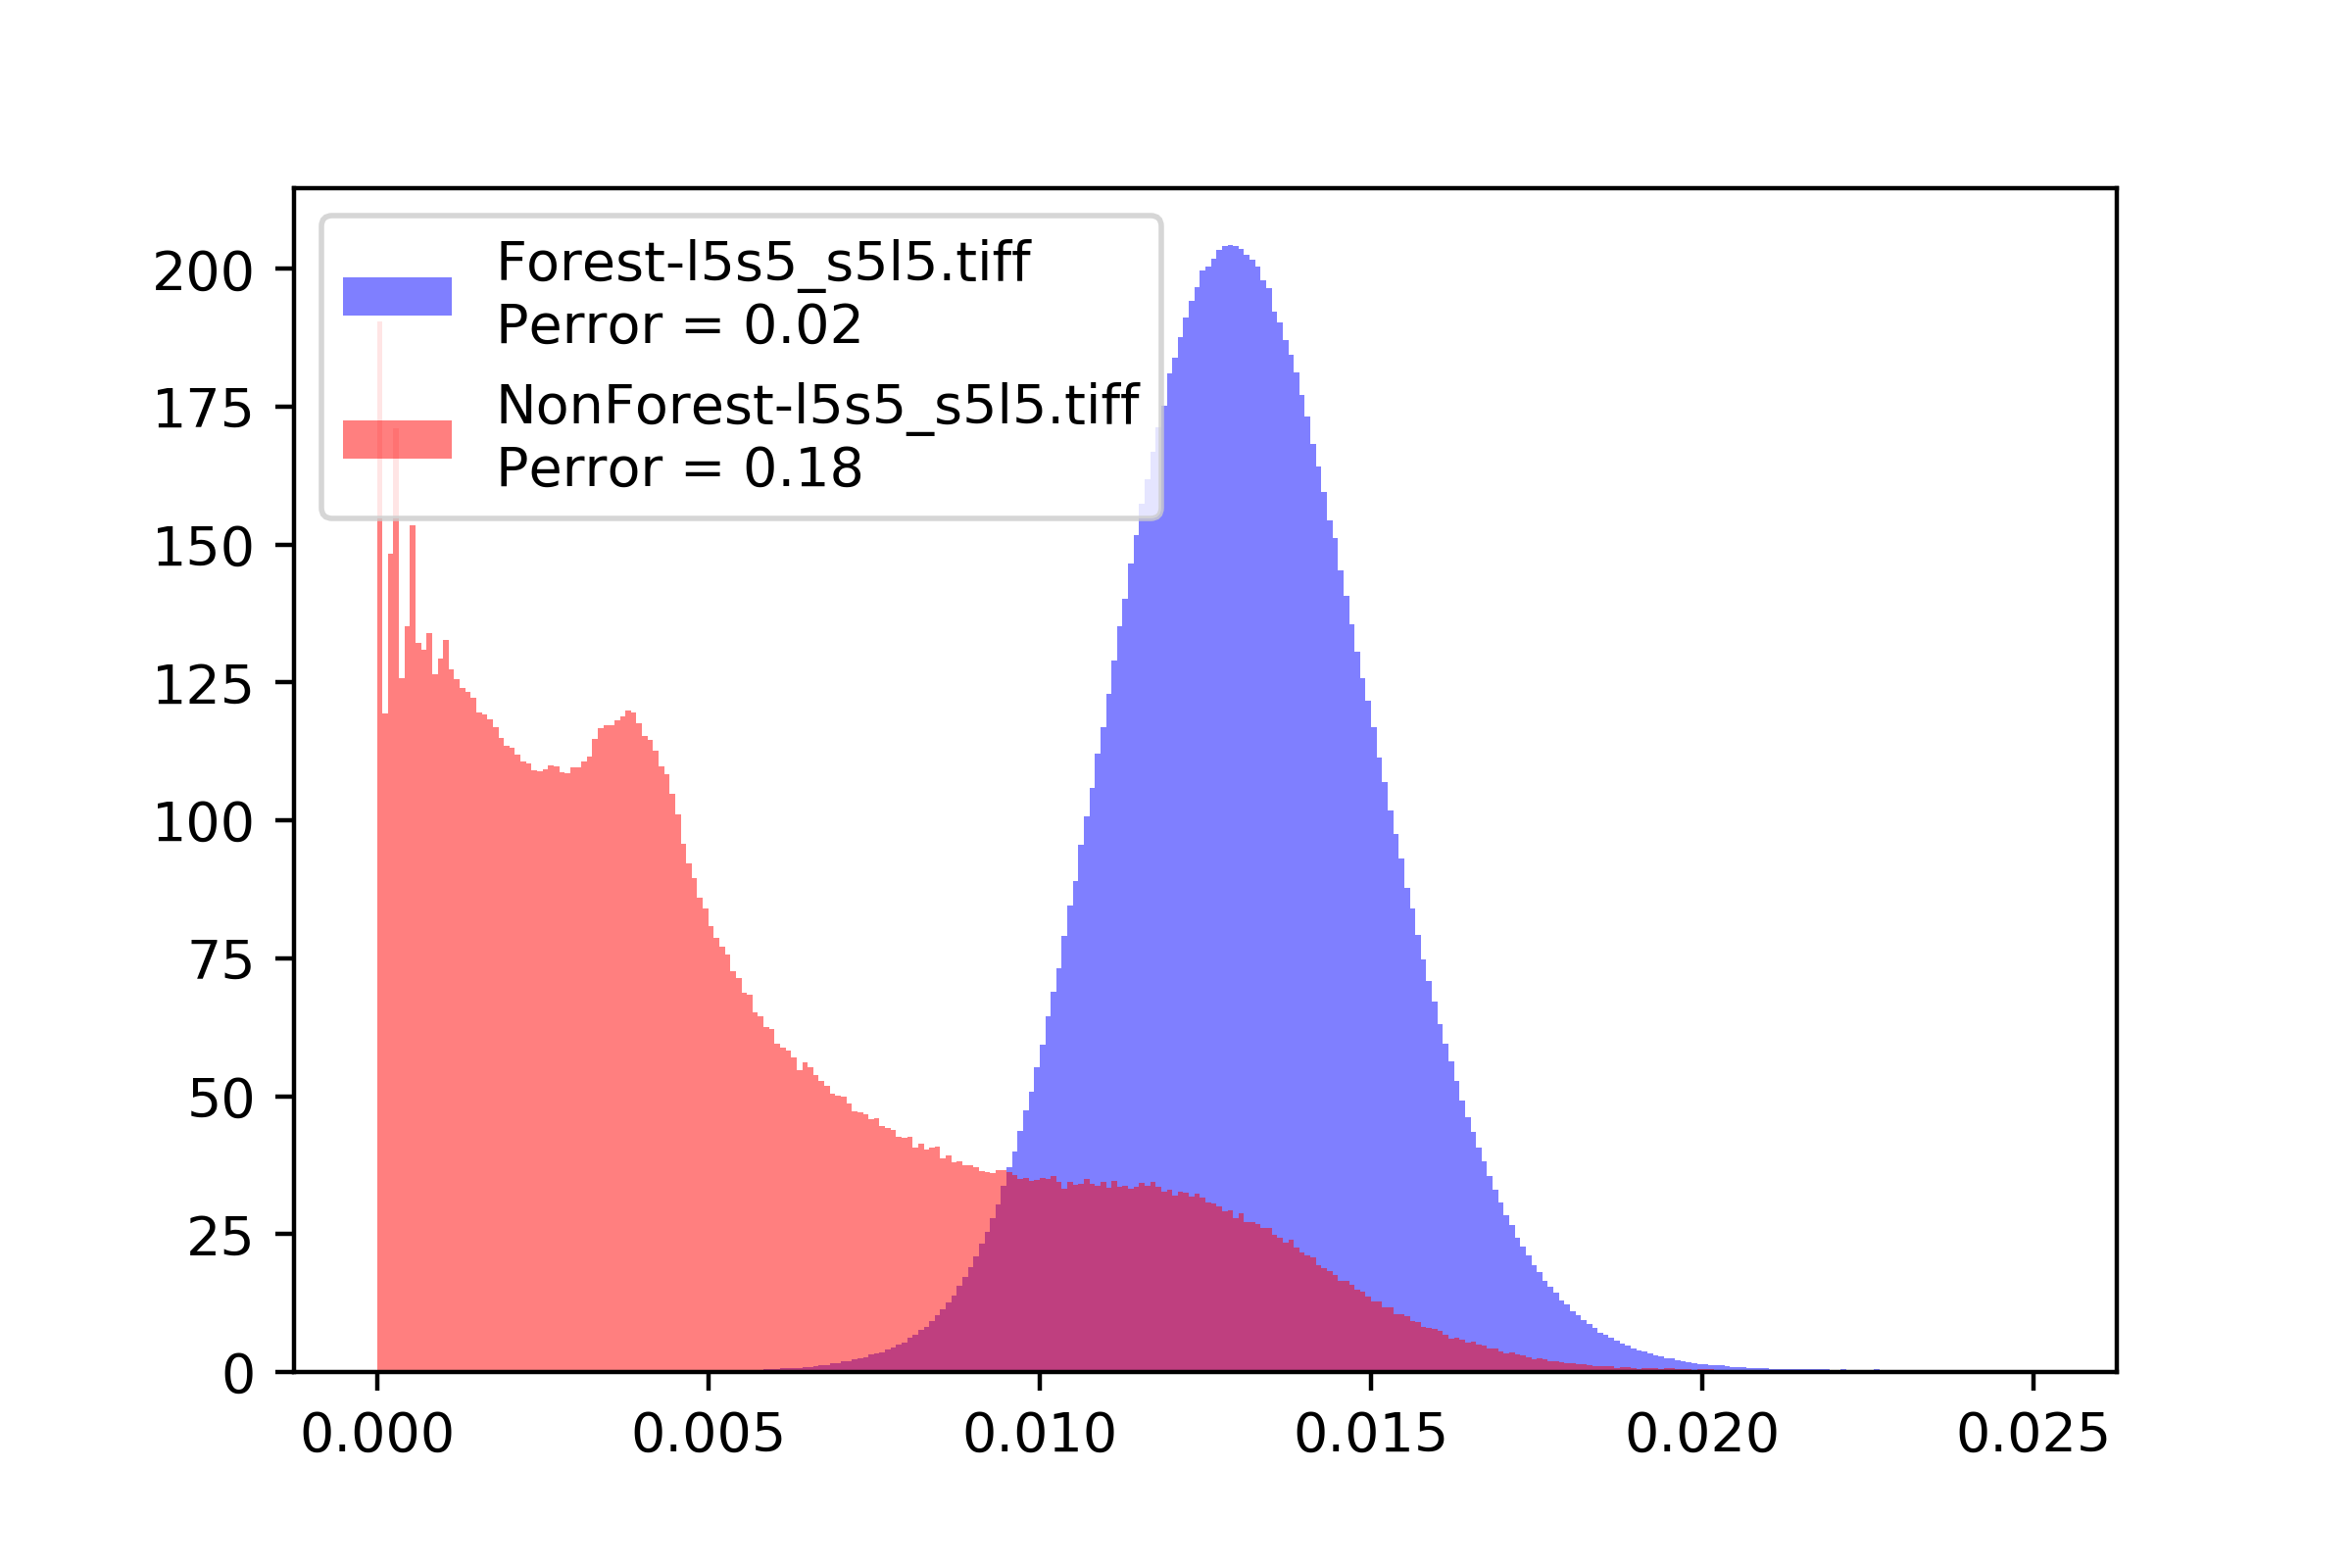
\includegraphics[width=\linewidth]{Chapter4/laws_textures/l5s5_s5l5.png}
     \caption{Probability density Function for l5s5/s5l5.}
  \end{subfigure}
  \centering
  \begin{subfigure}[b]{0.4\linewidth}
    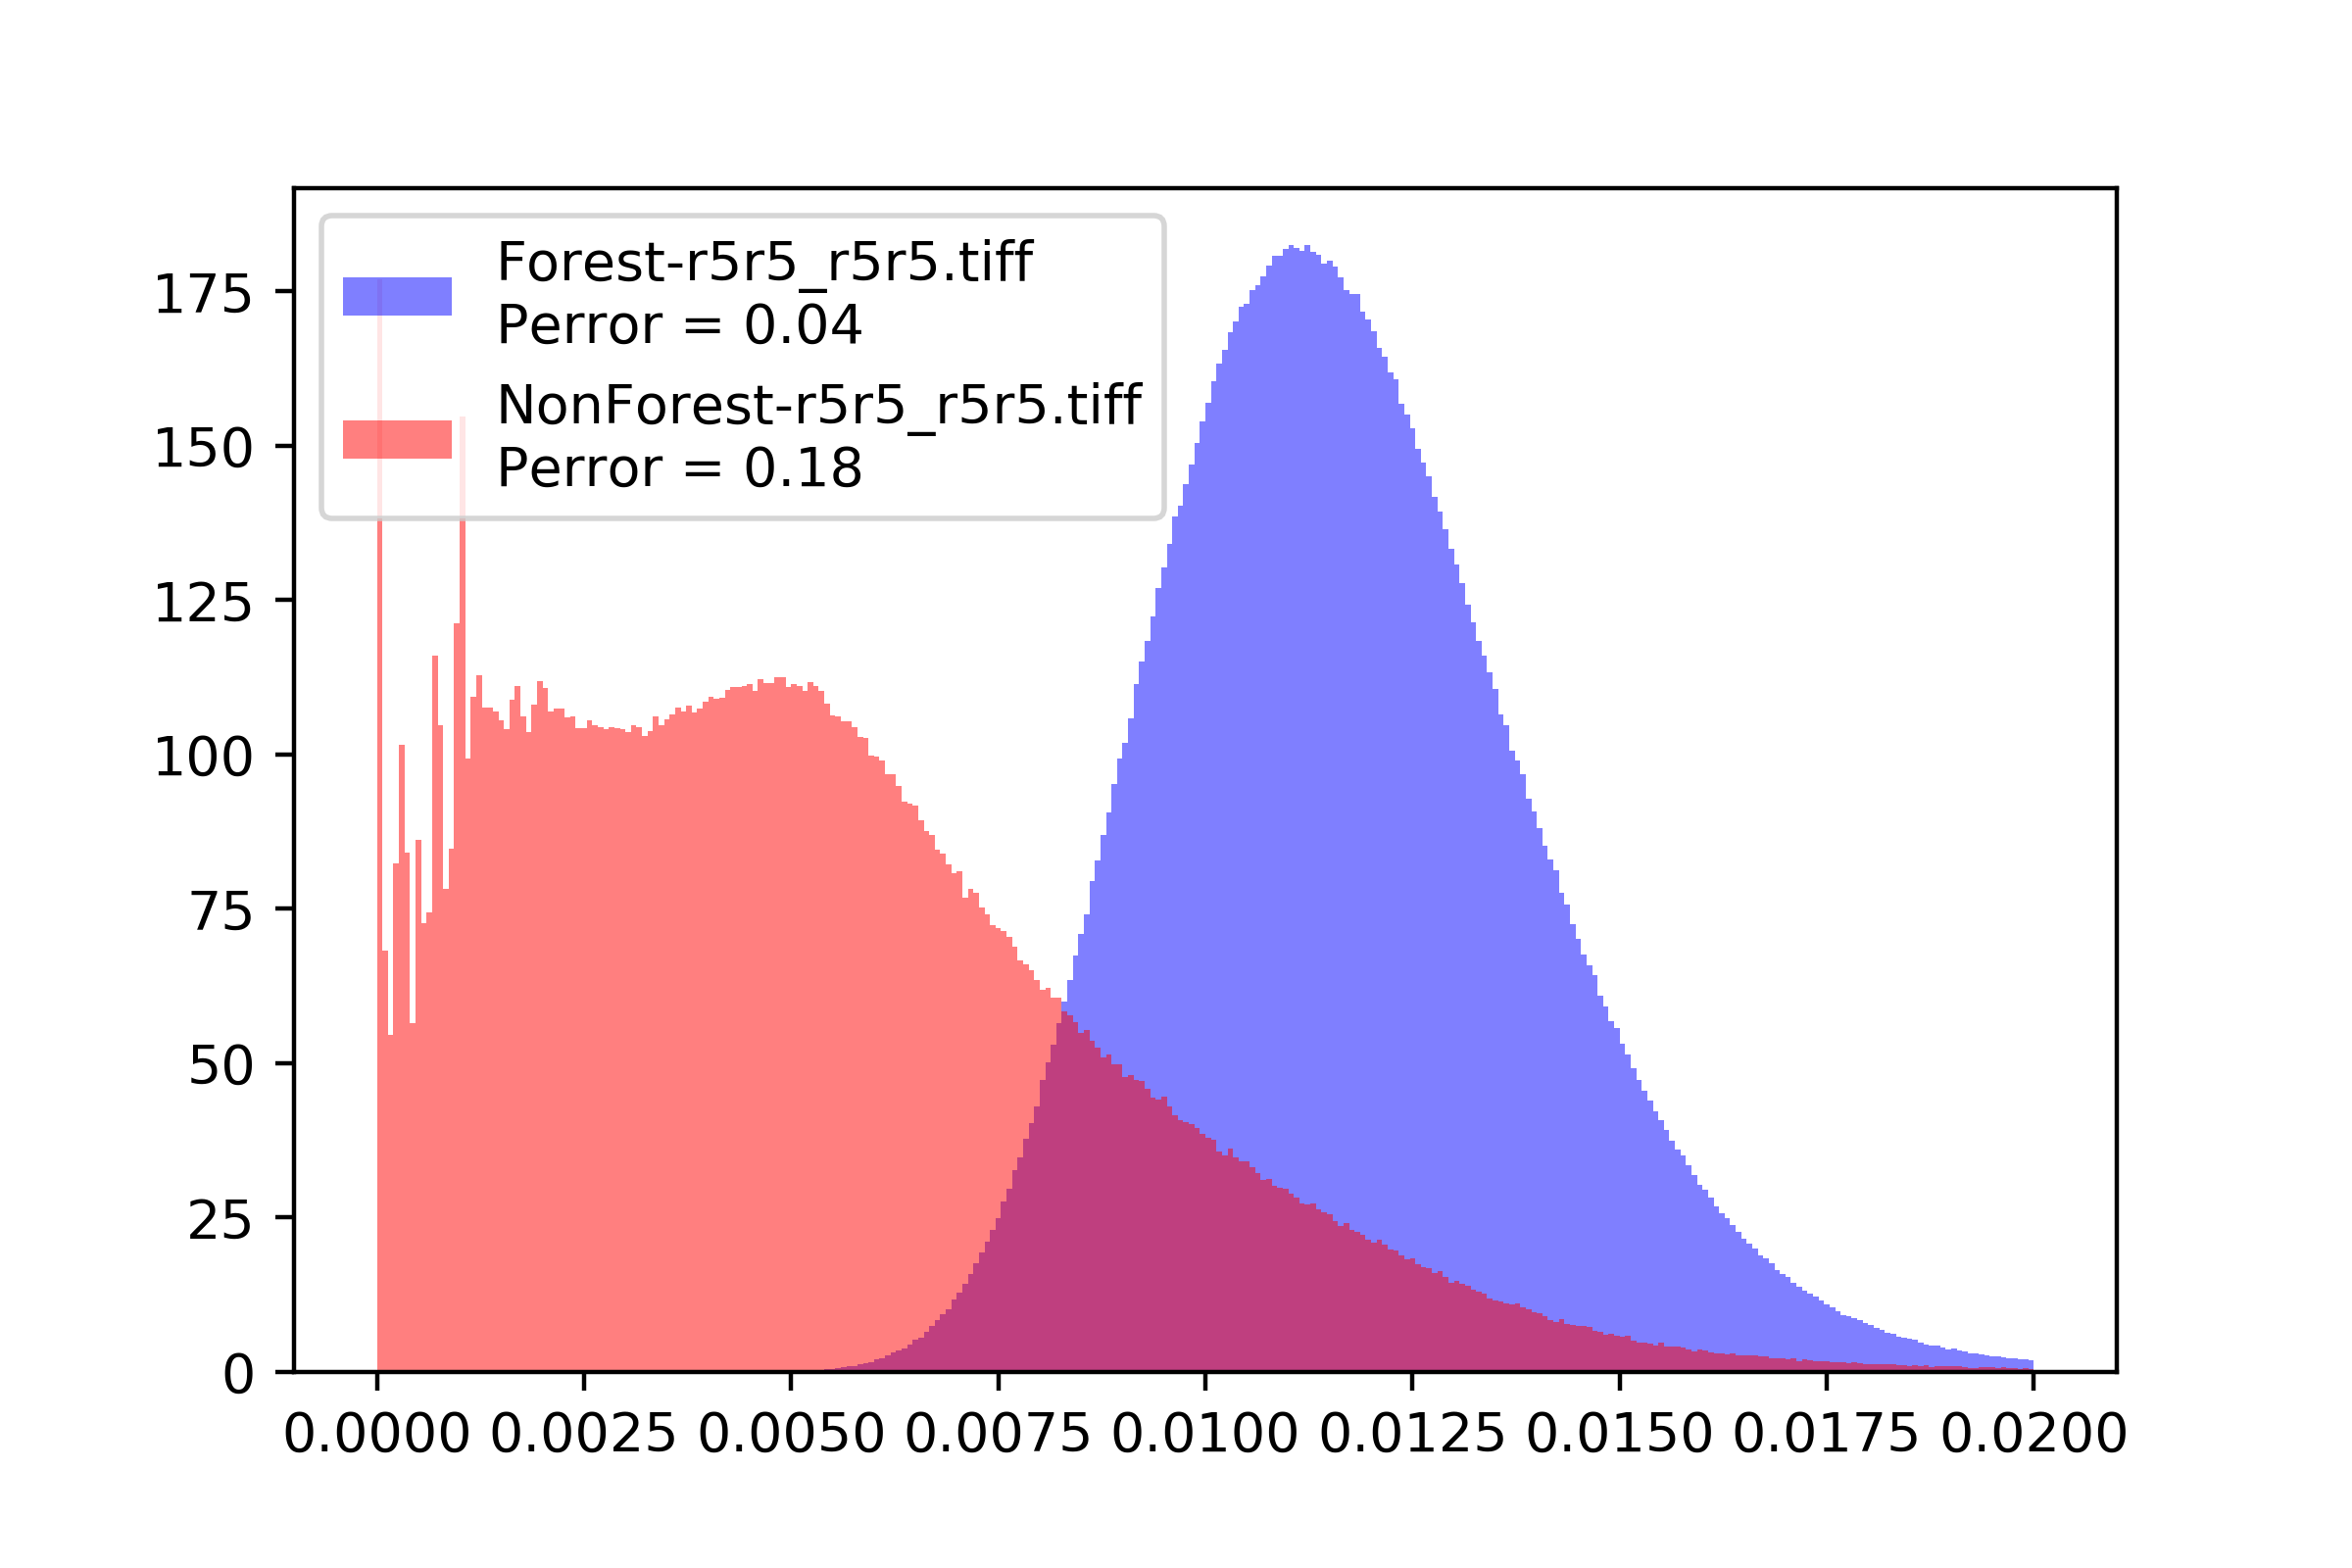
\includegraphics[width=\linewidth]{Chapter4/laws_textures/r5r5_r5r5.png}
     \caption{Probability density Function for r5r5/r5r5.}
  \end{subfigure}
  \centering
  \begin{subfigure}[b]{0.4\linewidth}
    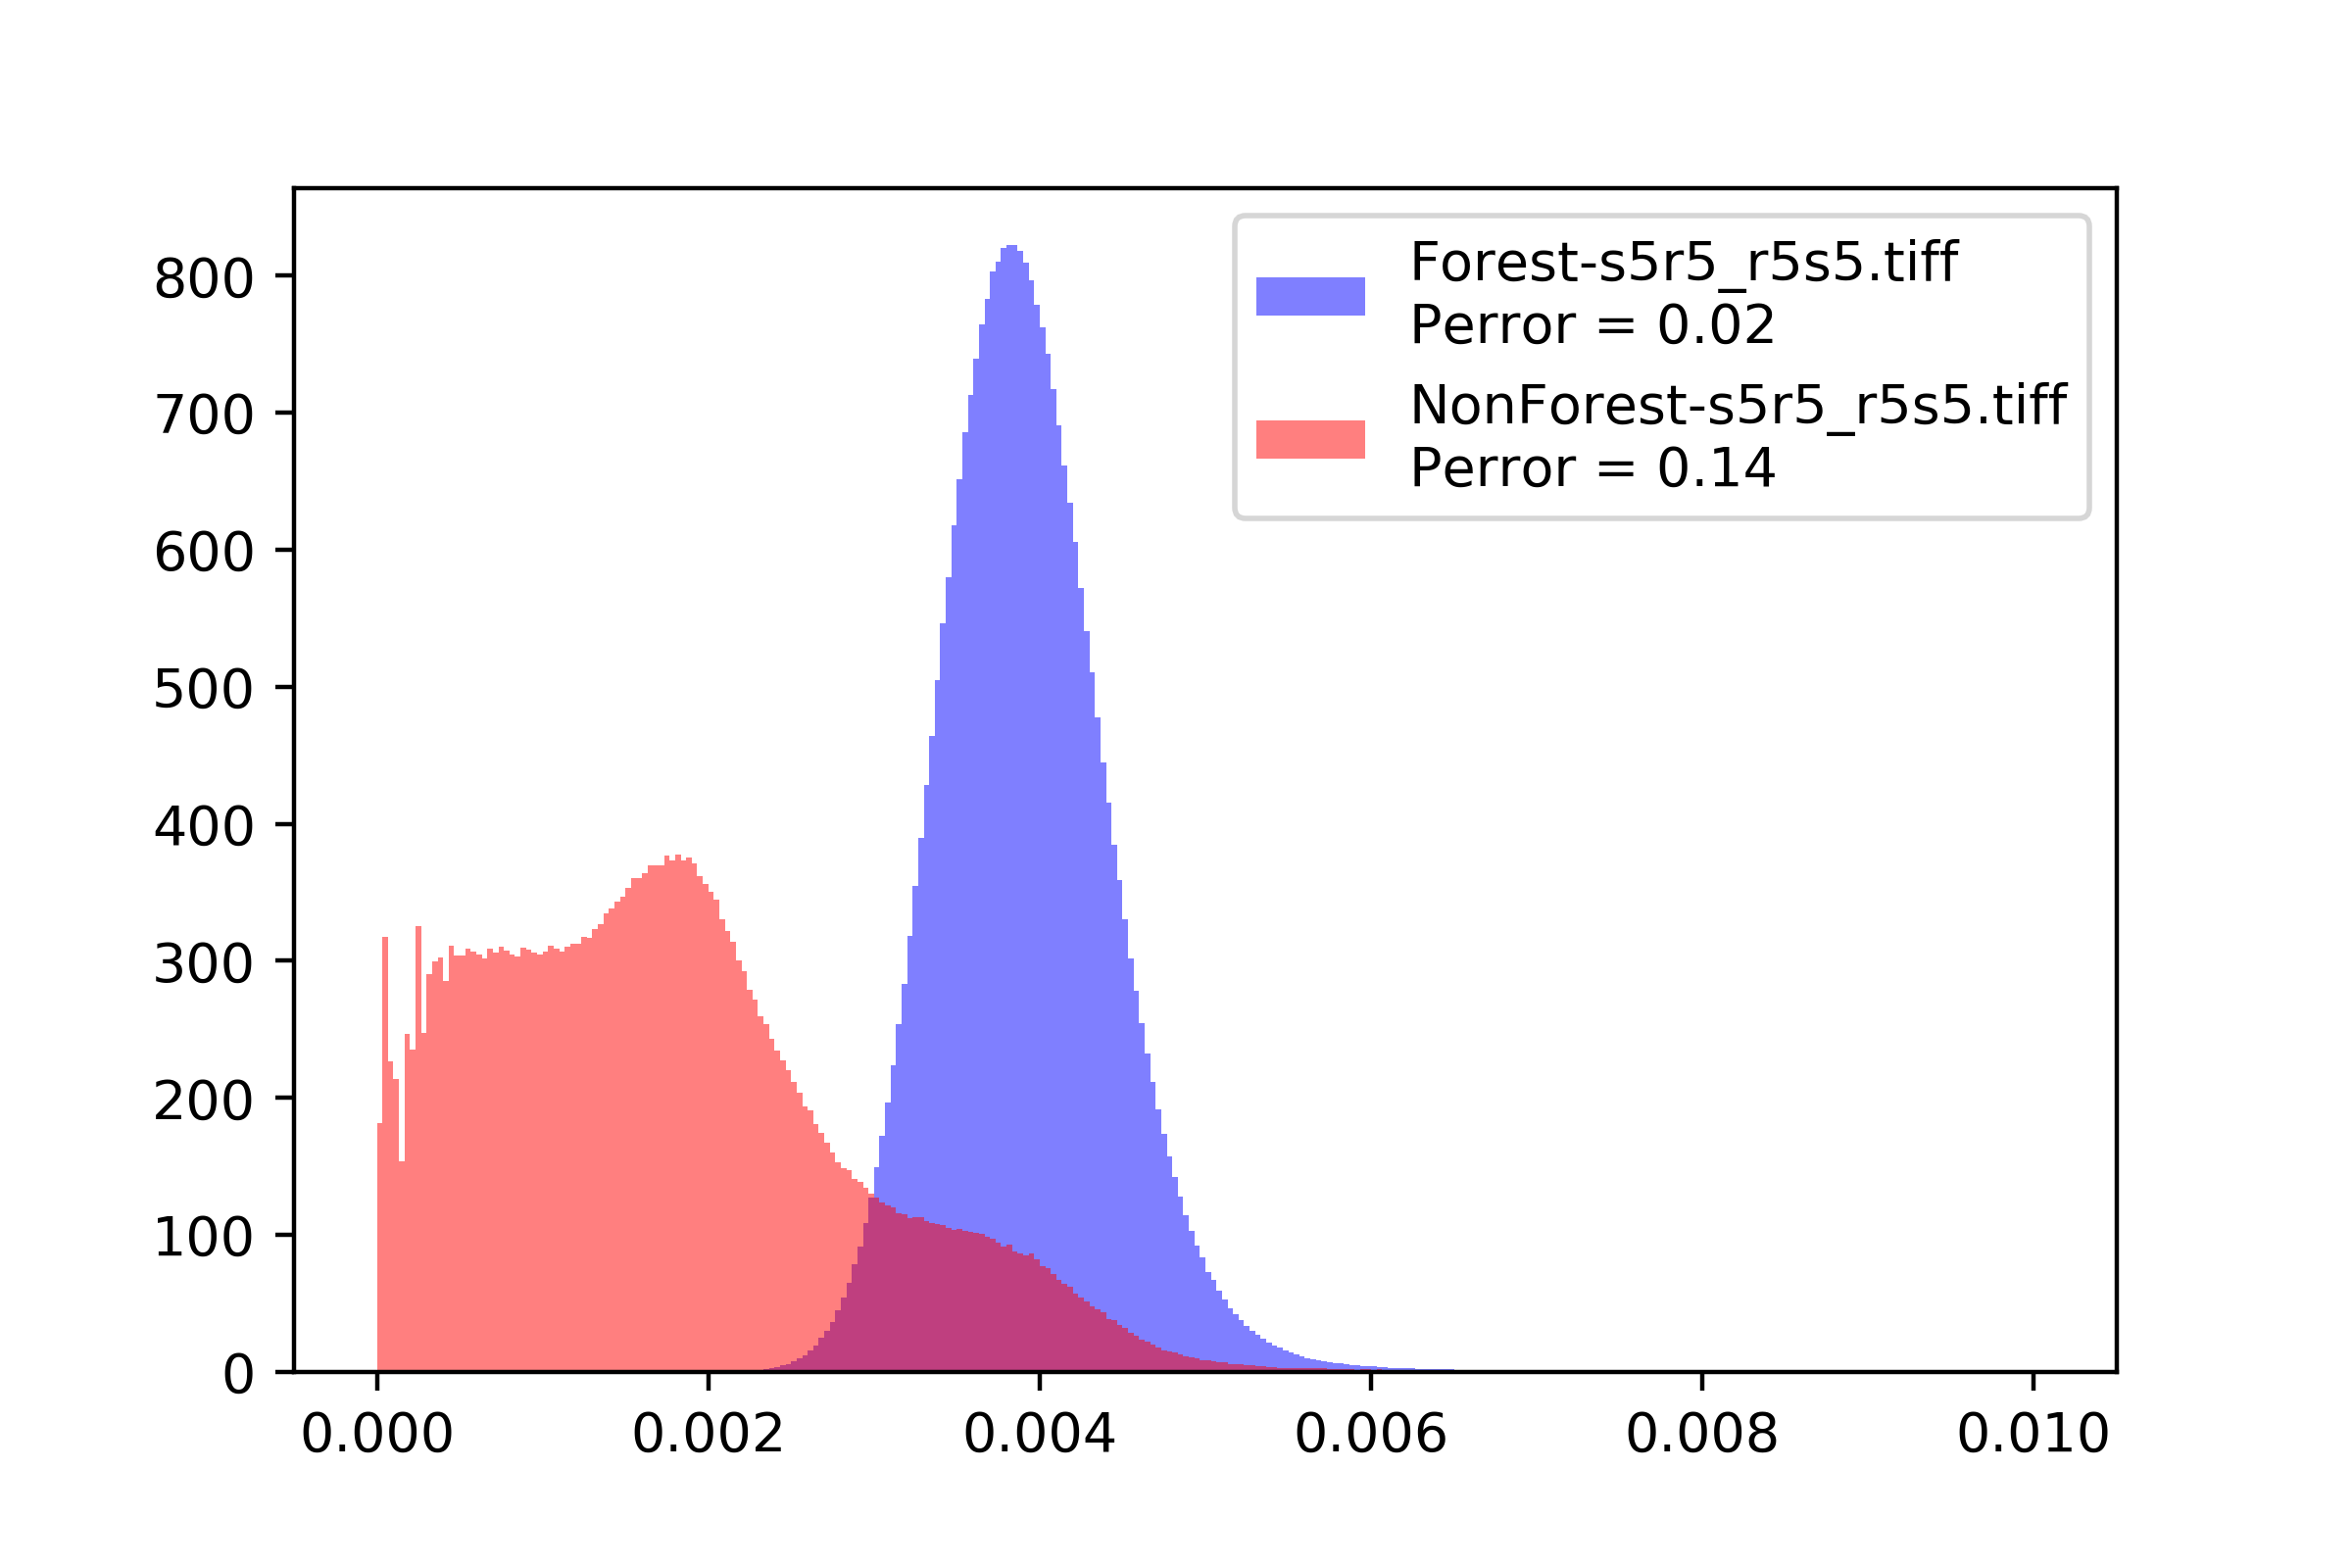
\includegraphics[width=\linewidth]{Chapter4/laws_textures/s5r5_r5s5.png}
     \caption{Probability density Function for s5r5/r5s5.}
  \end{subfigure}
\end{figure}

\newpage
\begin{figure}[H]
  \centering
  \begin{subfigure}[b]{0.4\linewidth}
    \includegraphics[width=\linewidth]{Chapter4/laws_textures/s5s5_s5s5.png}
     \caption{Probability density Function for s5s5/s5s5 texture.}
  \end{subfigure}
\end{figure}




From the images above we can see clearly that the PDFs are more separated than the coherence PDF. A important thing that must be noticed is that all the different textures have very similar PDFs, which might me an indicator that the images are very similar between themselves, and that using more than one texture for classification means adding redundant information for the classification algorithms, which might degrade performance instead of increasing it.

\section{Sum And Difference Histograms Textures}
\label{sec:sum_and_diff_hist_textures}
The last method analyzed for generating textures is the Sum and Difference Histogram Texture. Below there are the texture results for this method.

\begin{figure}[H]
  \centering
  \begin{subfigure}[b]{0.4\linewidth}
    \includegraphics[width=\linewidth]{Chapter4/sum_and_diff_textures/cluster_prominenceimage.png}
     \caption{Cluster Prominence Texture Image}
  \end{subfigure}
  \centering
  \begin{subfigure}[b]{0.4\linewidth}
    \includegraphics[width=\linewidth]{Chapter4/sum_and_diff_textures/cluster_shadeimage.png}
     \caption{Cluster Shade Texture Image}
  \end{subfigure}
  \centering
  \begin{subfigure}[b]{0.4\linewidth}
    \includegraphics[width=\linewidth]{Chapter4/sum_and_diff_textures/contrastimage.png}
     \caption{Contrast Texture Image}
  \end{subfigure}
  \centering
  \begin{subfigure}[b]{0.4\linewidth}
    \includegraphics[width=\linewidth]{Chapter4/sum_and_diff_textures/correlationimage.png}
     \caption{Correlation Texture Image}
  \end{subfigure}
\end{figure}
\newpage
\begin{figure}[H]\ContinuedFloat
  \centering
  \begin{subfigure}[b]{0.4\linewidth}
    \includegraphics[width=\linewidth]{Chapter4/sum_and_diff_textures/energyimage.png}
     \caption{Energy.}
  \end{subfigure}
  \centering
  \begin{subfigure}[b]{0.4\linewidth}
    \includegraphics[width=\linewidth]{Chapter4/sum_and_diff_textures/entropyimage.png}
     \caption{Entropy Texture Image}
  \end{subfigure}
  \centering
  \begin{subfigure}[b]{0.4\linewidth}
    \includegraphics[width=\linewidth]{Chapter4/sum_and_diff_textures/homogeneityimage.png}
     \caption{ Homogeneity Texture Image}
  \end{subfigure}
  \centering
  \begin{subfigure}[b]{0.4\linewidth}
    \includegraphics[width=\linewidth]{Chapter4/sum_and_diff_textures/meanimage.png}
     \caption{Mean Texture Image}
  \end{subfigure}
\end{figure}
\newpage
\begin{figure}[H]\ContinuedFloat
  \centering
  \begin{subfigure}[b]{0.4\linewidth}
    \includegraphics[width=\linewidth]{Chapter4/sum_and_diff_textures/varianceimage.png}
     \caption{Variance Texture Image}
  \end{subfigure}
\end{figure}
Again we must analyze the histograms to see if these features really are useful for classification and segmentation of a image.

\begin{figure}[H]
  \centering
  \begin{subfigure}[b]{0.4\linewidth}
    \includegraphics[width=\linewidth]{Chapter4/sum_and_diff_textures/cluster_prominence_hist.png}
     \caption{Probability density Function for Cluster Prominence.}
  \end{subfigure}
  \centering
  \begin{subfigure}[b]{0.4\linewidth}
    \includegraphics[width=\linewidth]{Chapter4/sum_and_diff_textures/cluster_shade_hist.png}
     \caption{Probability density Function for Cluster Shade.}
  \end{subfigure}
  \centering
  \begin{subfigure}[b]{0.4\linewidth}
    \includegraphics[width=\linewidth]{Chapter4/sum_and_diff_textures/contrast_hist.png}
     \caption{Probability density Function for Contrast.}
  \end{subfigure}
  \centering
  \begin{subfigure}[b]{0.4\linewidth}
    \includegraphics[width=\linewidth]{Chapter4/sum_and_diff_textures/correlation_hist.png}
     \caption{Probability density Function for Correlation.}
  \end{subfigure}
  \centering
  \begin{subfigure}[b]{0.4\linewidth}
    \includegraphics[width=\linewidth]{Chapter4/sum_and_diff_textures/energy_hist.png}
     \caption{Probability density Function for Energy.}
  \end{subfigure}
  \centering
  \begin{subfigure}[b]{0.4\linewidth}
    \includegraphics[width=\linewidth]{Chapter4/sum_and_diff_textures/entropy_hist.png}
     \caption{Probability density Function for Entropy.}
  \end{subfigure}
\end{figure}

\begin{figure}[H]\ContinuedFloat

  \centering
  \begin{subfigure}[b]{0.4\linewidth}
    \includegraphics[width=\linewidth]{Chapter4/sum_and_diff_textures/homogeneity_hist.png}
     \caption{Probability density Function for Homogeneity.}
  \end{subfigure}
  
  \centering
  \begin{subfigure}[b]{0.4\linewidth}
    \includegraphics[width=\linewidth]{Chapter4/sum_and_diff_textures/mean_hist.png}
     \caption{Probability density Function for Mean.}
  \end{subfigure}
  
  \centering
  \begin{subfigure}[b]{0.4\linewidth}
    \includegraphics[width=\linewidth]{Chapter4/sum_and_diff_textures/variance_hist.png}
     \caption{Probability density Function for Variance.}
  \end{subfigure}
  
\end{figure}

From the histograms and the texture images it is clear that some of the textures are excellently suited for classification, specially the Cluster Shade and Cluster Prominence textures which provide excellent separation between the probability density function. From those images it is clear that in the case of the TANDEM-X the sum and difference histogram methods for texture provided a significantly better result than the other textures, so through the rest of the work there will be a focus in using this method instead of the others, since due to computational limitations is not viable to use all texture methods for classification, since it takes a very long time to compute them.


\chapter{Classification Results}
\label{cap:classification_results}
%%%%%%%%%%%%%%%%%%%%%%%%%%%%%%%%%%%%%%%%%%%%%%%%%%%%%%%%%%%%%%%%%%%%%%%%%%%%%%%%
%2345678901234567890123456789012345678901234567890123456789012345678901234567890
%        1         2         3         4         5         6         7         8
% THESIS CHAPTER

% short summary of the chapter
\section*{Summary}
In this chapter we will show the results of classification without the textures and compare it with the results of classification using the additional textures features. It will be shown the results for classification for forest and deforested areas in the Amazon Rain forest looking at acquisitions from the TANDEM-X satellite. Besides that, it will be also shown classification results using the acquisitions of the SENTINEL1 satellite for areas in the Amazon Rain forest, and compare the results with textures and without textures.



\section{TANDEM-X Data Analysis} 
\label{sec:gv2}
On this section it will be analyzed the result of textures for the volumetric correlation of a acquisition of the TANDEM-X satellite. The volumetric correlation image can be seen below.
From this image, the textures were made using the sum and difference histogram method and it was given as a input to a Random Forest algorithm for classification. The random forest was trained using the reference map provided by DLR. Due to computational limitations not all textures were used, but just some of them. The textures choice was based on the PDFs of different classes. The textures chosen as input to the Random Forest algorithms were: Cluster Shade, Cluster Prominence, Contrast, Variance. Besides that, the coherence was also given as an input to the Random Forest Algorithm. The classification results with the textures can be seen below.

\begin{figure}[H]
  \centering
  \begin{subfigure}[b]{0.4\linewidth}
    \includegraphics[width=\linewidth]{Chapter5/coSSC_master_gamma_vol.pdf}
     \caption{Volumetric Correlation image of TANDEM-X acquisition}
  \end{subfigure}
  \begin{subfigure}[b]{0.4\linewidth}
    \includegraphics[width=\linewidth]{Chapter5/TANDEM-X/classification_resultsimage.pdf}
    \caption{Random Forest Results with Texture}
  \end{subfigure}
  \caption{Volumetric Correlation and Classification.}
  \label{fig:classification_tandem}
\end{figure}

On the volumetric correlation image above the white pixels have higher correlation, which indicate the presence of a deforested area, while the dark pixels have a lower correlation, which is characteristic of a forested area. On the right it is possible to see the classification result given by the random forest. On the classification image on the right the white pixels indicate deforested area while the green pixels indicate the presence of a forested area. \\
It is clear from \figref{fig:classification_tandem} that the classification is accurate, but it is not possible to see how accurate the result is. Due to this it was also obtained the accuracy results when compared to the reference map provided by DLR %\figref{fig:reference_map}
. The accuracy results with different combinations of textures can be seen in the table below

\begin{table}[H]
\centering
\begin{tabular}{ |c |c |}
 \hline
     Variance & 46.78\% \\
     Coherence & 4.70\% \\
     Variance/Coherence & 4.70\% \\
     Cluster Prominence & 3.82\% \\
     Cluster Prominence/Variance & 4.17\% \\
     Cluster Prominence/Coherence & 3.80\% \\
     Cluster Prominence/Variance/Coherence & 4.70\% \\
     Cluster Shade & 1.33\% \\
     Cluster Shade/Variance & 1.30\% \\
     Cluster Shade/Coherence & 1.30\% \\
     Cluster Shade/Variance/Coherence & 1.30\% \\
     Cluster Shade/Cluster Prominence & 1.27\% \\
     Cluster Shade/Cluster Prominence/Variance & 1.26\% \\
     Cluster Shade/Cluster Prominence/Coherence & 1.26\% \\
     Cluster Shade/Cluster Prominence/Variance/Coherence & 1.28\% \\
     Contrast & 21.13\% \\
     Contrast/Variance & 21.07\% \\
     Contrast/Coherence & 5.18\% \\
     Contrast/Variance/Coherence & 4.70\% \\
     Contrast/Cluster Prominence & 4.42\% \\
     Contrast/Cluster Prominence/Variance & 3.81\% \\
     Contrast/Cluster Prominence/Coherence & 3.47\% \\
     Contrast/Cluster Prominence/Variance/Coherence & 3.47\% \\
     Contrast/Cluster Shade & 1.30\% \\
     Contrast/Cluster Shade/Variance & 1.30\% \\
     Contrast/Cluster Shade/Coherence & 1.30\% \\
     Contrast/Cluster Shade/Variance/Coherence & 1.40\% \\
     Contrast/Cluster Shade/Cluster Prominence & 1.15\% \\
     Contrast/Cluster Shade/Cluster Prominence/Variance & 1.52\% \\
     Contrast/Cluster Shade/Cluster Prominence/Coherence & 1.47\% \\
     Contrast/Cluster Shade/Cluster Prominence/Variance/Coherence & 1.29\% \\
 \hline
\end{tabular}
\caption{Error results with different textures combinations}
\label{table:accuracy_results_tandem}
\end{table}

From the table \ref{table:accuracy_results_tandem} we can quantitatively see how much was the improvement. Trying to run a classification using just the Coherence as an input gives a classification error of 4.70\%, while if all textures are used then the error drops to 1.29\%, in a way that the error 3 times smaller than the original error. Keep in mind that the classification map provided by DLR is not 100\% accurate, so these numbers are not 100\% accurate and have a small error, which might explain why using just 2 textures, the cluster shade and cluster prominence, gives a smaller error (1.27\%) than using the 4 textures together with the coherence (1.28\%).

Even though this improvement might seem surprising it is important to notice that the coherence image used was a high quality image acquired with ideal conditions and with a height of ambiguity that yields a clear separation between the forest and deforested areas, but normally the SARs acquisitions are not always this good for classification, specially if it is not used a double satellite system like TANDEM-X (which has the advantage of not having temporal decorrelation between images since they are taken at the same time).
On the next section this method will be used on acquisitions that are not so suited to make a classification in order to see the improvement that the textures can provide in non-ideal conditions.

\section{Sentinel1 Data Analysis}

As said previously, the TANDEM-X images used for classification were taken in ideal conditions, in a way that making a classification on that image only is easy and even if no textures are used the classification results can provide a high accuracy. \newline
The advantage of the TANDEM-X satellite is that it is twin satellite system that fly together taking pictures of the same area at the same time, in a way that the temporal decorrelation does not affect these images. \newline
But normally, the pictures taken with SARs radars are taken at different days, in a way that the temporal changes on the scene strongly affects the image. \newline
To illustrate this, on this section it will be shown coherence images of images of the satellite SENTINEL1, which have a 6 days temporal baseline between acquisitions. There were 5 images that were used to make the classification on this example, taken at the days 25/04/2019, 01/05/2019, 07/05/2019, 13/05/2019/ and 19/05/2019. Due to computational limitations it was chosen to make the mean between the images, since making the textures of each image might take a long time. The images have a 12m pixel resolution and cover an area of almost $40000km^2$, so making the textures of each image can take until 50 hours. \newline
From the acquisitions it is possible to extract the brightness ($\sigma^0)$ of the scene and since there are 5 images it is possible to get 4 coherence images with a 6 days temporal baseline. Even though it is also possible to get the coherence at 12, 18 and 24 days it was chosen not to do so, since the images with such temporal baseline will provide little to no useful information for classification.
Below there are images of the average $\sigma^0$ and the average coherence $\gamma$ of the acquisitions.
\begin{figure}[H]
    \centering
    \includegraphics[width=0.75\linewidth]{Chapter5/SENTINEL1/geo_cohimage.pdf}
    \caption{$\gamma$ acquisition.}
    \label{fig:gamma_sentinel}
\end{figure}{}
\begin{figure}[H]
    \centering
    \includegraphics[width=0.75\linewidth]{Chapter5/SENTINEL1/geo_temp_sigma0dbimage.pdf}
    \caption{$\sigma^0$ acquisition.}
    \label{fig:sigma_sentinel}
\end{figure}{}

\newpage
The respective histograms for the coherence and $\sigma^0$ can be seen below.

\begin{figure}[H]
  \centering
  \begin{subfigure}[b]{0.4\linewidth}
    \includegraphics[width=\linewidth]{Chapter5/SENTINEL1/Coherence/cluster_prominence_histogram.pdf}
     \caption{Probability density Function for Cluster Prominence.}
  \end{subfigure}
  \centering
  \begin{subfigure}[b]{0.4\linewidth}
    \includegraphics[width=\linewidth]{Chapter5/SENTINEL1/Coherence/cluster_shade_histogram.pdf}
     \caption{Probability density Function for Cluster Shade.}
  \end{subfigure}
  \centering
  \begin{subfigure}[b]{0.4\linewidth}
    \includegraphics[width=\linewidth]{Chapter5/SENTINEL1/Coherence/contrast_histogram.pdf}
     \caption{Probability density Function for Contrast.}
  \end{subfigure}
  \centering
  \begin{subfigure}[b]{0.4\linewidth}
    \includegraphics[width=\linewidth]{Chapter5/SENTINEL1/Coherence/correlation_histogram.pdf}
     \caption{Probability density Function for Correlation.}
  \end{subfigure}
  \centering
  \begin{subfigure}[b]{0.4\linewidth}
    \includegraphics[width=\linewidth]{Chapter5/SENTINEL1/Coherence/energy_histogram.pdf}
     \caption{Probability density Function for Energy.}
  \end{subfigure}
  \centering
  \begin{subfigure}[b]{0.4\linewidth}
    \includegraphics[width=\linewidth]{Chapter5/SENTINEL1/Coherence/entropy_histogram.pdf}
     \caption{Probability density Function for Entropy.}
  \end{subfigure}
\end{figure}

\begin{figure}[H]\ContinuedFloat
  \centering
  \begin{subfigure}[b]{0.4\linewidth}
    \includegraphics[width=\linewidth]{Chapter5/SENTINEL1/Coherence/homogeneity_histogram.pdf}
     \caption{Probability density Function for Homogeneity.}
  \end{subfigure}
  
  \centering
  \begin{subfigure}[b]{0.4\linewidth}
    \includegraphics[width=\linewidth]{Chapter5/SENTINEL1/Coherence/mean_histogram.pdf}
     \caption{Probability density Function for Mean.}
  \end{subfigure}
  
  \centering
  \begin{subfigure}[b]{0.4\linewidth}
    \includegraphics[width=\linewidth]{Chapter5/SENTINEL1/Coherence/variance_histogram.pdf}
     \caption{Probability density Function for Variance.}
  \end{subfigure}
  \caption{Histograms of Coherence Textures.}
  \label{fig: sentinel_coherence_hist}
\end{figure}
\newpage


\begin{figure}[H]
  \centering
  \begin{subfigure}[b]{0.4\linewidth}
    \includegraphics[width=\linewidth]{Chapter5/SENTINEL1/Sigma0/cluster_prominence_histogram.pdf}
     \caption{Probability density Function for Cluster Prominence.}
  \end{subfigure}
  \centering
  \begin{subfigure}[b]{0.4\linewidth}
    \includegraphics[width=\linewidth]{Chapter5/SENTINEL1/Sigma0/cluster_shade_histogram.pdf}
     \caption{Probability density Function for Cluster Shade.}
  \end{subfigure}
  \centering
  \begin{subfigure}[b]{0.4\linewidth}
    \includegraphics[width=\linewidth]{Chapter5/SENTINEL1/Sigma0/contrast_histogram.pdf}
     \caption{Probability density Function for Contrast.}
  \end{subfigure}
  \centering
  \begin{subfigure}[b]{0.4\linewidth}
    \includegraphics[width=\linewidth]{Chapter5/SENTINEL1/Sigma0/correlation_histogram.pdf}
     \caption{Probability density Function for Correlation.}
  \end{subfigure}
  \centering
  \begin{subfigure}[b]{0.4\linewidth}
    \includegraphics[width=\linewidth]{Chapter5/SENTINEL1/Sigma0/energy_histogram.pdf}
     \caption{Probability density Function for Energy.}
  \end{subfigure}
  \centering
  \begin{subfigure}[b]{0.4\linewidth}
    \includegraphics[width=\linewidth]{Chapter5/SENTINEL1/Sigma0/entropy_histogram.pdf}
     \caption{Probability density Function for Entropy.}
  \end{subfigure}
  \centering
\end{figure}

\begin{figure}[H]\ContinuedFloat
    \centering
    \begin{subfigure}[b]{0.4\linewidth}
        \includegraphics[width=\linewidth]{Chapter5/SENTINEL1/Sigma0/homogeneity_histogram.pdf}
        \caption{Probability density Function for Homogeneity.}
    \end{subfigure}
  
  \centering
  \begin{subfigure}[b]{0.4\linewidth}
    \includegraphics[width=\linewidth]{Chapter5/SENTINEL1/Sigma0/mean_histogram.pdf}
    \caption{Probability density Function for Mean.}
  \end{subfigure}
  \centering

    \centering
    \begin{subfigure}[b]{0.4\linewidth}
        \includegraphics[width=\linewidth]{Chapter5/SENTINEL1/Sigma0/variance_histogram.pdf}
        \caption{Probability density Function for Variance.}
        \end{subfigure}
    \caption{Histograms of $\sigma^0$ Textures.}
    \label{fig: sentinel_sigma_hist}
\end{figure}

From the images and the histograms above it is clear that it is harder to make a classification, as the $\sigma^0$ and $\gamma$ are not as separated as TANDEM-X acquisition.
\begin{figure}[H]
    \centering
    \includegraphics[width=\linewidth]{Chapter5/TANDEM-X/reference_mapimage.pdf}
    \caption{Reference Map provided by DLR. The Green pixels represent forest pixels and white pixels represent deforested pixels.}
    \label{fig:ref_sentinel}
\end{figure}{}

Below it is possible to see the classification result using only the coherence and the $\sigma^0$ as input to the random forest.
\begin{figure}[H]
    \centering
    \includegraphics[width=\linewidth]{Chapter5/TANDEM-X/result_no_texturesimage.pdf}
    \caption{Classification Results without textures. The Green pixels represent forest pixels and white pixels represent deforested pixels.}
    \label{fig:result_no_textures_sentinel}
\end{figure}{}
It is clear from that image the limitations of the machine learning algorithms for classification, since the classification clearly has a low accuracy. Below it is possible to see the random forest result using the textures.

\begin{figure}[H]
    \centering
    \includegraphics[width=\linewidth]{Chapter5/TANDEM-X/result_texturesimage.pdf}
    \caption{Classification Results with textures. The Green pixels represent forest pixels and white pixels represent deforested pixels.}
    \label{fig:result_textures_sentinel}
\end{figure}{}

From that new image it is now clear how powerful the textures can be in aiding classification algorithms.
For comparison, below it is also attached the optical image of the area acquired via Google Earth. The area acquired with Sentinel1 is show in the red square.

\begin{figure}[H]
    \centering
    \includegraphics[width=\linewidth]{Chapter5/real_image_google_earth.pdf}
    \caption{Google Earth image of analysed area.}
    \label{fig:google_earth_area_sentinel1}
\end{figure}{}

\section{Performance of Random forest and parameters tuning}
There are 3 important parameters that have great impact on the performance of the Random Forest algorithm:
\begin{itemize}
    \item Number of estimators: The number of trees in the forest.
    \item Maximum depth: The maximum depth of the tree
    \item Minimum samples for leaf: The minimum number of samples required to be at a leaf node. A split point at any depth will only be considered if it leaves at the minimum number of samples for leaf training samples in each of the left and right branches
\end{itemize}{}

Even though increasing those parameters can lead to greater accuracy, there are some breaking points in which the accuracy decreases, and there are some points in which the accuracy is stagnated and will not further increase, therefore only wasting computational time for no valuable return. For example, one might think that increasing the depth of the tree would yield a greater accuracy, but there is a limit in which the results will not improve, but it will take more time for the algorithm to make the training and the classification.
Below there area images that show how the accuracy of the classification algorithm changes with variations on the parameters:
\begin{figure}[H]
    \centering
    \includegraphics[width=\linewidth]{Chapter5/Number_of_estimators.png}
    \caption{Accuracy versus number of estimators for different tree depths.}
    \label{fig:num_estimators}
\end{figure}{}

\begin{figure}[H]
    \centering
    \includegraphics[width=\linewidth]{Chapter5/number_of_leaves.png}
    \caption{Accuracy versus minimum number of samples for leaf parameter.}
    \label{fig:num_leaves}
\end{figure}{}


\chapter{Application of Textural methods to Change Detection Algorithms}
\label{cap:carabas_chapter}
\section{Summary}
This chapter will present the change detection problem for targets concealed by a forest. It will 
also present the SAR system that was used to perform the data acquisition and the dataset that was created by this system.
The dataset consists of SAR images collected that the Swedish low VHF-band SAR system CARABAS-II. 
The images were made publicly available by the Swedish Airforce Research center with the purpose of fostering research on the 
subject field of target detection under tree foliage. 


\section{Wavelength Resolution SAR Systems}
Wavelength resolution SAR images are radar systems with resolution in the order of 
the radar system Wavelength. According to \cite{62}, the resolution of a cell of a SAR image can be
calculated by:

\begin{equation}
    \delta = \frac{\lambda_c c}{4 \theta_H B}
\end{equation}

where $\lambda_c$ is the wavelength corresponding to the radar central frequency, $\theta_H$
is the aperture angle (in radians), $c$ is the speed of light and $B$ is the system bandwidth.

It is obvious that the backscatter characteristcs of the SAR depends on the frequency band of the system.
For wavelength-resolution SAR systems there is a significant difference between the backscatter of targets with size the order
of the wavelength - which present the resonance scattering phenomena \cite{63} - and targets small compared to the wavelength - which present
the the Rayleigh scattering phenomena \cite{63}. 

According to (17ref), Wavelength SAR systems are not sensitive to small scatterers inside the resolution cell,
thus the scattering process is mainly due to scatterers with dimensions in the order of the system wavelength.
Since the resolution of the cell is similar to the resolution of the scatterer, there can be only one single scatterer inside each cell, 
therefore the image will not be greatly affected by speckle noise (speckle noise is a major cause of problems in non wavelength-resolution SAR still). For example, according to \cite{64}
in frequencies below 100 MHz, in forest areas, the backscatter is dominated by backscattering from tree foliage.

Moreover, scatterers that are large tend to be static objects, hence a stack of images of the same area will present a high degree of 
similarity between multi-pass acquisitions. Therefore regular noise redution techniques do not have to be applied when dealing with those set of images \cite{ 61}.

It is also worth mentioning that according to \cite{ 66}, signal attenuation in low-frequency wavelength-resolution SAR systems 
is not a major concern. Studies \cite{63} have also shown that signal attenuation can be as little as 3dB in low-frequency SAR acquisitions in forest areas.


Due to all that, according to (63ref), low resolution SAR systems are better suited to Foliage Penetrating (FOPEN) applications.
Also according to (63ref), VHF-band is the optimal radar system for FOPEN applications for vehicle-sized target detection.

\section{The CARABAS-II Challenge Problem}
There are many situations were there is a need for monitoring vehicles concealed by foliage over a large area.
For example, for military applications, it might be necessary to monitor the positioning of enemy vehicles trespassing
a restricted area. For environmental purposes it might be needed to pinpoint the position of vehicles that are being used
for illegal deforestation over protected forests. If SARs are to be used for such purposes, it is ideal that low frequency systems
are chosen since those provide a wide survaillance area and good foliage penetration capabilities. 
At low frequency (VHF-band) the main backscatter from the target area is due to large scatterers, e.g. tree canopy, houses,
vehicles, and other man-made objects, which will appear as very bright objects in the image.

The challenge related to change detection is associated with the trade-off between having high accuracy detection and high false alarm rate.
Normally what happens is by trying to increase the overall accuracy of detection algorithms will incur in having a high number of false alarms, 
therefore when designing an algorithm for detection it is necessary to have both good detection capabilities and a low enough false alarm rate
to be used by the client. In foliage penetration applications, the main source of clutter comes from large tree trunks, and the more sparse the
forest is the less will be the number of false targets. It is also true that the larger the tree then the higher will be the number of false alarms \cite{Book_ML}.

The objects that will be used to assess the quality of the change detection method will be a set of 25 military vehicles distributed among a testing area.
Since those objects are large (compared to the bandwidth of the signal), and stationary, then their radar signature will be very stable between acquisitions.
This will be used as an advantage by taking acquisitions with different flight passes to supress clutter noise from tree canopy.

According to (ref 1/2 challenge) VHF-band has good performance for detecting targets under trees, but there are very few VHF SAR systems in the world.
To overcome this problem researchers from the FOI released a VHF-band SAR image dataset to the public to foster the developement of 
change detection methods for wavelengh-resolution SAR systems in VHF band, which is the dataset that will be used in this work.


\section{The CARABAS-II System}

The CARABAS-II is the second generation SAR system designed by the Swedish Defense Research Agency (FOI) for FOPEN applications.
The CARABAS-II has participated in numerous military campaigns and has been used for reasearch purpose since the nineties.
The radar is a VLF UHB SAR system that transmits HH-polarized radio waves in the frequency range of 
20-90 MHz, therefore having resolution in the range of 3.3-15 m. The radar antenna is mounted on a Sabreliner aircraft as seen in \figref{fig:sabreliner}.

\begin{figure}[h]
    \centering
    \includegraphics{chapter6/sabreliner.jpg}
    \caption{The CARABAS-II VHF SAR mounted in front of a Sabreliner airplane}
    \label{fig:sabreliner}
\end{figure}

In the table below the system parameters for the CARABAS-II system are presented for the
flight campaigns that were used in this work. 

\begin{table}[h]
    \centering
    \begin{tabular}{|c|c|}
        \hline
        System Parameters & Values \\ \hline
        Nominal flight altitude & 3 - 9 km \\ \hline
        Nominal flight speed & 127 m/s \\ \hline
        Frequency band & 20-86 MHz \\ \hline
        Aperture angle & 90 degrees \\ \hline
        Transmitted power & 500 W \\ \hline
        Pulse modulation & Non-linear frequency modulation \\ \hline
        Radio Frequency Interference (RFI) sniff & On \\ \hline
        Frequency sub-bands & 35 (36 with RFI-sniff \\ \hline
        Frequency step & 1.875 Mhz \\ \hline
        Center frequencies & 21.25-85Mhz \\ \hline
        Pulse repetition & frequency 5000Hz \\ \hline
        Pulse length & 15$\mu$s \\ \hline
        Maximum range & 26.4 km \\ \hline
    \end{tabular}
    \caption{CARABAS-II SAR system parameters. Source: (76 ref)}
    \label{tab:carabas_system}
\end{table}

\section{The CARABAS-II Dataset}

By trying to promote research on change detection algorithms for wavelength-resolution
images, FOI created a dataset of images acquired by CARABAS-II and made it publicly available. 
This dataset is the one used to test and assess the quality of the proposed CDA.

The dataset consists of 24 SAR images selected from over 150 images obtained during different flight campaigns.
Each image covers the same ground area of 6 $km^2$ (3 km vertically and 2 km horizontally)
and is given in the form of a 3000 X 2000 matrix, where each pixel size is 1km x 1km.
According to \cite{ 77,62,78} the images are already calibrated, pre-processed and geocoded.

The location of the image dataset is inside the military base station Missile Test Area North
Vidsel in northern Sweden in 2002. The test site is a region near the village of Nausta \cite{ 75}.
The vegetation of the area is dominated by Scots Pine tree \cite{ 76}, which consists of small and medium size trees.
According to \cite{75} the area also contains fields, roads and lakes.

With the objective of testing CDA quality, it was deployed 25 testing targets over the testing with different configuration 
and arrangements. The testing targets consists of ten TGB11 model military vehicles, eight TGB30 model 
military vehicles, and seven TGGB40 model military vehicles. The dimensions of each vehicle are presented in the table (numero).
From the table (numero) it can be seen that the dimensions of the vehicles are similar to the wavelength of the CARABAS-II system,
therefore all advantages of targets with similar dimension to the wavelength previously mentioned hold true for the dataset.

\begin{table}[h]
    \centering
    \begin{tabular}{|c|c|c|c|c|}
        \hline
        Military Vehicle & Lenght & Width & Height & Quantity \\ \hline
        TGB11 & 4.4 m & 1.9 m & 2.2 m & 10 \\ \hline
        TGB30 & 6.8m & 2.5m & 3.0 m & 8 \\ \hline
        TGB40 & 7.8m & 2.5m & 3.0m & 7 \\ \hline
    \end{tabular}
    \caption{Target dimensions}
    \label{tab:vehicle_dimensions}
\end{table}


The dataset of 24 images were acquired using four different flight passes. Each 
flight pass has an incidence angle of 58 degrees, used the StripSAR mode and was acquired with the radar looking left \cite{ 75,76}.
The vehicles were positioned in two diferent forests, Forest 2 being in the northwest of the field, and forest 1 being in the
southeast of the test area. 

\begin{figure}[h]
    \centering
    \includegraphics{chapter6/carabas_vehicles_fisico.jpg}
    \caption{Military vehicles used as target. Left:TGB11. Middle:TGB30. Right:TGB40. 
    This picture also depicts the vegetation characteristics of the test area}
    \label{fig:veiculos}
\end{figure}

The vehicles in mission 2 are positioned in forest 2 and have a heading angle of 225 degrees pointing southwest direction;
vehicles in mission 3 are positioned in forest 2 and have a heading angle of 315 degrees pointing northwest direction;
vehicles in mission 4 are located in forest 1 and have the same heading angle of mission 2;
vehicles in mission 5 are located in forest 1 and have a heading angle of 270 degrees pointing west direction.
Vehicles in mission 2 and 3 are separated approximately by 50m, as such for vehicles in mission 4 and 5.
\figref{fig:carabas_vehicles} presents images of each mission with the vehicles area highlighted in red.

\begin{figure}[h]
    \centering
    \includegraphics{chapter6/carabas_vehicles.jpg}
    \caption{Examples of CARABAS-II images where (a) is mission 2, (b) is mission 3, (c) is mission 4 and (d)
    is mission 5}
    \label{fig:carabas_vehicles}
\end{figure}

In table \ref{tab:flight_mission} it is presented the summary with the information of each image in the dataset

\begin{table}[H]
    \centering
    \begin{tabular}{|c|c|c|c|c|}
        \hline
        Image Number & Mission & Pass & Flight Heading (degrees) & Target Heading \\ \hline
        1 & 2 & 1 & 225 & 225  \\ \hline
        2 & 2 & 2 & 135 & 225  \\ \hline
        3 & 2 & 3 & 225 & 225  \\ \hline
        4 & 2 & 4 & 135 & 225 \\ \hline
        5 & 2 & 5 & 230 & 225 \\ \hline
        6 & 2 & 6 & 230 & 225 \\ \hline
        7 & 3 & 1 & 225 & 315 \\ \hline
        8 & 3 & 2 & 135 & 315 \\ \hline
        9 & 3 & 3 & 225 & 315 \\ \hline
        10 & 3 & 4 & 135 & 315 \\ \hline
        11 & 3 & 4 & 135 & 315 \\ \hline
        12& 3 & 6 & 230 & 315  \\ \hline
        13 & 4 & 1 & 225 & 225  \\ \hline
        14 & 4 & 2 & 135 & 225  \\ \hline
        15 & 4 & 3 & 225 & 225  \\ \hline
        16 & 4 & 4 & 135 & 225  \\ \hline
        17 & 4 & 5 & 230 & 225  \\ \hline
        18 & 4 & 6 & 230& 225 \\ \hline
        19 & 5 & 1 & 225 & 270  \\ \hline
        20 & 5 & 2 & 135 & 270  \\ \hline
        21 & 5 & 3 & 225 & 270  \\ \hline
        22 & 5 & 4 & 135 & 270  \\ \hline
        23 & 5 & 5 & 230 & 270  \\ \hline
        24 & 5 & 6 & 230 & 270  \\ \hline
    \end{tabular}
    \caption{Measurements parameters for each image}
    \label{tab:flight_mission}
\end{table}

\section{Traditional Change Detecion in Wavelength-Resolution SAR Images}

The field of FOPEN target detection using wavelength-resolution SAR images (both in VHF and UHF bands) has been 
around of decades \cite{ 25,48,79,80}. Among those studies, the CARABAS-II system dataset was used in many different FOPEN studies 
\cite{}. 

As previously mentioned, the objective of the study is to create a change detection method that will compare 
different images of the same target field (in this case, the forests in Sweden) and try to identify the targets that 
have changed position in the image (in this case, the military vehicles TGB11, TGB30 and TGB40 ) and give the exact location of the vehicle positions.


There are several change detection methods that were already used in the CARABAS-II dataset.
The first method that yielded accuracy high enough for real world applications was based in Bayes linear classification \cite{81}.
After that, a myriad of new methods were proposed, such as: Likelihood-ratio test (LRT) \cite{ 61}, combination of LRT and Space-Time 
adaptative processing (STAP) \cite{ 76} among others. Traditionally CDAs were also mainly based on traditional statistical decision theory, e.g., 
traditional hypothesis testing criterion methods, such as maximum a posteriori 
criterion \cite{Book_Kay}, likelihood ratio test \cite{LRT1,LRT2,LRT3}, generalized likelihood ratio test \cite{GLRT1,GLRT2,GLRT3}, 
or Bayesian theory approaches \cite{Bayes1, Bayes2}. Several of those CDAs have achieved high accuracy 
in terms of true positives, but most show unsatisfactory performance in terms of false positives percentage \cite{Carabas, Ricardo,LucasRamos,Chris}.








% \chapter{Methodology}
% Given the information presented here on this work on SARs and land cover classification, the objective of this graduation thesis is to study techniques on classification maps generation and information extraction based on modelling the temporal decorrelation of SAR images, focusing specifically on the SENTINEL-1 satellite. The data for this SAR was provided by DLR.

With the objective of improving land cover classification, different methods for temporal decorrelation were studied and analysed in partnership with DLR, until a final method was chosen and used throughout the rest of the work. 

Chapter one was the background information on SAR principles and coherence estimation. On this chapter it was presented the main bibliography on SAR and coherence estimation and the problem was briefly explained. On chapter two the problem on temporal decorrelation modelling was explained with more depth and it was explained how using these decorrelation models could be useful for improving land cover classification techniques. On chapter three it was presented not only the methods used for tackling the problem but also how to implement it, including the pipelines important for the data processing.

The programming tools chosen for solving the problem and validating it were Python and C++. These tools were chosen based on versatility, how easy they are to implement using these languages and computational time for the programs.

% \chapter{Final Remarks}
% \label{cap:comentarios finais}
% The table below shows the schedule proposed for the development and finalization of the Bachelor's Thesis.
\begin{figure}[H]
    \centering
    \includegraphics[width=1.1\linewidth]{Final Remarks/tabela.png}
    \caption{Proposed schedule for graduation thesis writing}
    \label{fig:tabela}
\end{figure}

Given the table above, it is clear that the development is according to the schedule proposed. A lot of the work has already been done, the remaining part being researching additional bibliographic references for the thesis, getting inputs from supervisor and writing the final paper.


% REFERENCIAS BIBLIOGRAFICAS
\renewcommand\bibname{\itareferencesnamebabel} %renomear título do capítulo referências
\bibliography{Referencias/referencias}

% apendices
%\appendix
%\chapter{Código \textit{Mathematica} desenvolvido} %opcional
%\label{appendix:apeA}
%\input{ApeA/apendiceA}

%\chapter{Geração da modulação digital}
%\label{appendix:apeB}
%\input{ApeB/apendiceB}

% % Glossario%
\itaglossary
\printglossary


% Folha de Registro do Documento
% Valores dos campos do formulario
\FRDitadata{15 de dezembro de 2020}
\FRDitadocnro{DCTA/ITA/TC-047/2020} %(o número de registro você solicita a biblioteca)
\FRDitaorgaointerno{Instituto Tecnológico de Aeronáutica -- ITA}
%Exemplo no caso de pós-graduação: Instituto Tecnol{\'o}gico de Aeron{\'a}utica -- ITA
\FRDitapalavrasautor{
Radares de abertura sintética; SAR; Land Cover Classification; Engenharia eletrônica; Machine Learning
}
\FRDitapalavrasresult{Radares de abertura sintética; Processamento de imagens; Aprendizagem (inteligência artificial);
Redes neurais; Algoritmos; Engenharia eletrônica.}
%Exemplo no caso de graduação (TG):
\FRDitapalavraapresentacao{ITA, São José dos Campos. Curso de Graduação em Engenharia Eletrônica. Orientador: Prof. Dr.
Marcelo da Silva Pinho. Publicado em 2020.}
%Exemplo no caso de pós-graduação (msc, dsc):
%\FRDitapalavraapresentacao{ITA, São José dos Campos. Curso de Graduação. Programa de Graduação em Engenharia Eletrônica. Área de Microondas e Optoeletrônica. Orientador: Prof.~José Edimar Barbosa Oliveira. Defesa em 25/06/2018. Publicada em 25/06/2018.}
\FRDitaresumo{%The focus of this work is to investigate how to best combine interferometric SAR (InSAR) images for land cover classification. The idea proposed takes advantage of multi-temporal data, acquired over short observation intervals (short-time-series). Images which were acquired with a larger temporal baseline are expected to have a larger interferometric coherence loss, while images acquired with a smaller temporal baseline are expected to have a higher correlation between them. The main idea of the work is to take advantage of the fact that different targets on the ground will temporally decorrelate at different rates. By modelling the temporal evolution of the temporal decorrelation it is possible to extract parameters numerically that can help classify the scene. By combining these parameters with other parameters of the scene, like backscatter, it is possible to use it as inputs for Machine Learning algorithms for classification, like Neural Networks or Random Forest (on this work Random Forest was chosen because it yielded a better result). The work was validated on the case of land cover classification over Europe(CORINE) and over the Amazon Rainforest, using Sentinel-1 C-band interferometric stacks which was provided by DLR. It was considered three different classes for this work: forested areas, non-forested areas and artificial surfaces.
%By comparing the result with the CORINE land cover map of 2012 the results show a level of agreement of 91\% and over 85\% for the Amazon Rainforest.}
%  Primeiro Parametro: Nacional ou Internacional -- N/I
%  Segundo parametro: Ostensivo, Reservado, Confidencial ou Secreto -- O/R/C/S
\FRDitaOpcoes{N}{O}
% Cria o formulario
\itaFRD

\end{document}
% Fim do Documento. O massacre acabou!!! :-)
